% !TeX program = xelatex
% !TeX encoding = UTF-8
% Presentazione revisionata: Iride: descrivere e visualizzare i dati
% Basata sul materiale originale fornito dall'autore e sul template M01_Pensare_con_i_dati.tex
% Compilazione: xelatex -interaction=nonstopmode Iride_M03_descrivere_visualizzare.tex (due passaggi)
% Diagrammi TikZ e figure statistiche vettoriali; sorgenti R e dati inclusi.
% Revisione completa delle 80 slide; fonti consultate il 18 novembre 2026.
\documentclass[12pt,aspectratio=1610]{beamer}
\geometry{paperwidth=20cm,paperheight=12.5cm}
\usepackage[italian,provide=*]{babel}
\usepackage{fontspec}
\IfFontExistsTF{NimbusSans-Regular.otf}{
\setsansfont{NimbusSans-Regular.otf}[BoldFont=NimbusSans-Bold.otf,ItalicFont=NimbusSans-Italic.otf,BoldItalicFont=NimbusSans-BoldItalic.otf]
\setmainfont{NimbusSans-Regular.otf}[BoldFont=NimbusSans-Bold.otf,ItalicFont=NimbusSans-Italic.otf,BoldItalicFont=NimbusSans-BoldItalic.otf]
}{
\setsansfont{TeX Gyre Heros}
\setmainfont{TeX Gyre Heros}
}
\IfFontExistsTF{DejaVu Sans Mono}{
\setmonofont{DejaVu Sans Mono}[Scale=.88]
}{\setmonofont{Latin Modern Mono}[Scale=.88]}
\usefonttheme{professionalfonts}
\usepackage{amsmath,amssymb,booktabs,array,graphicx,tikz,bookmark}
\usetikzlibrary{calc,positioning,arrows.meta}
\graphicspath{{Risorse/Figure/}}
\definecolor{Paper}{HTML}{F8F6F1}
\definecolor{Ink}{HTML}{253344}
\definecolor{Navy}{HTML}{15283E}
\definecolor{Quantum}{HTML}{5146A5}
\definecolor{Classical}{HTML}{087C74}
\definecolor{Muted}{HTML}{657180}
\definecolor{Rule}{HTML}{D6DAD9}
\definecolor{Night}{HTML}{112236}
\definecolor{Lilac}{HTML}{ABB5FF}
\definecolor{Mint}{HTML}{72D8C8}
\setbeamercolor{background canvas}{bg=Paper}
\setbeamercolor{normal text}{fg=Ink}
\setbeamertemplate{navigation symbols}{}
\setbeamertemplate{headline}{}
\setbeamertemplate{footline}{}
\setbeamersize{text margin left=0pt,text margin right=0pt}
\hypersetup{colorlinks=true,linkcolor=Classical,urlcolor=Classical,pdfpagemode=UseOutlines,pdfstartview=Fit,
 pdftitle={Iride: descrivere e visualizzare i dati},pdfauthor={Marzio De Corato},
 pdfsubject={Modulo M03: distribuzioni, confronti e rappresentazioni, Revisione completa: diagrammi TikZ, formule e codice R commentato}}
\bookmarksetup{open,openlevel=0,depth=2}
\newsavebox{\BodyBox}
\newsavebox{\SideBox}
\newsavebox{\RecallBox}
\newsavebox{\TitleBox}
\newcommand{\MeasureBox}[2]{\typeout{REVIEWBOX:#1:\the\wd#2:\the\ht#2:\the\dp#2}}

% Revisione completa: diagrammi TikZ, formalismo e box R.
\usepackage[most]{tcolorbox}
\usepackage{listings}
\usetikzlibrary{fit,backgrounds,matrix,decorations.pathreplacing}
\definecolor{GeoA}{HTML}{1D7890}
\definecolor{GeoB}{HTML}{C57E42}
\definecolor{GeoC}{HTML}{7363AA}
\definecolor{GeoTint}{HTML}{F0F4F3}
\lstdefinestyle{GeoR}{language=R,basicstyle=\ttfamily\fontsize{9.2}{12.2}\selectfont,
 keywordstyle=\color{Quantum}\bfseries,commentstyle=\color{Classical},stringstyle=\color{GeoB},
 numbers=left,numberstyle=\tiny\color{Muted},numbersep=4pt,showstringspaces=false,
 columns=fullflexible,keepspaces=true,breaklines=true,xleftmargin=1.15em,
 frame=none,aboveskip=0pt,belowskip=0pt,tabsize=2}
\newsavebox{\PilotLeftBox}
\newsavebox{\PilotRightBox}
\newcommand{\PLabel}[1]{\par{\color{Classical}\bfseries\fontsize{9}{11}\selectfont\MakeUppercase{#1}}\par\vspace{1.8mm}}
\newcommand{\PBody}[1]{\par{\fontsize{11.3}{14.8}\selectfont #1\par}}
\newcommand{\PSmall}[1]{\par{\fontsize{9.8}{13.1}\selectfont #1\par}}
\newcommand{\PCode}[2]{%
\begin{tcolorbox}[enhanced,arc=1.8mm,boxrule=.65pt,
  colback=white,colframe=Classical!75!Navy,colbacktitle=Navy,
  coltitle=white,fonttitle=\bfseries\fontsize{9.6}{12}\selectfont,
  title={#1},left=1.7mm,right=1.3mm,top=1.5mm,bottom=1.3mm,
  before skip=1mm,after skip=1mm]
\lstinputlisting[style=GeoR]{Codice/#2}
\end{tcolorbox}}
\newcommand{\PInfo}[1]{%
\begin{tcolorbox}[enhanced,arc=1.6mm,boxrule=.55pt,colback=GeoTint,
 colframe=Rule!80!Classical,left=2.3mm,right=2.3mm,top=2mm,bottom=2mm,
 before skip=1mm,after skip=1mm]
\PSmall{#1}\end{tcolorbox}}
\tikzset{
 pFlow/.style={draw=Classical!45,fill=white,rounded corners=2mm,
  line width=.7pt,align=center,minimum height=1.1cm,font=\sffamily\fontsize{10}{12}\selectfont},
 pEdge/.style={-{Latex[length=2.3mm]},draw=Classical,line width=.95pt},
 pGroup/.style={draw=Rule,fill=white,rounded corners=2mm,line width=.65pt},
 pDotA/.style={circle,fill=GeoA,inner sep=1.25pt},
 pDotB/.style={circle,fill=GeoB,inner sep=1.25pt},
 pDotC/.style={circle,fill=GeoC,inner sep=1.25pt}
}
\newcommand{\PilotChrome}[4]{%
  \node[anchor=north west,inner sep=0,text width=17.7cm] at ([xshift=.95cm,yshift=-.55cm]current page.north west) {\color{Navy}\bfseries\fontsize{20.6}{24.5}\selectfont #1};
  \node[anchor=north east,inner sep=0] at ([xshift=19.05cm,yshift=-.14cm]current page.north west) {\color{Classical}\fontsize{8}{10}\selectfont\hyperlink{slide2}{#2}};
  \draw[Classical,line width=1.2pt] ([xshift=.95cm,yshift=-1.7cm]current page.north west)--([xshift=2.35cm,yshift=-1.7cm]current page.north west);
  \draw[Rule,line width=.65pt] ([xshift=.95cm,yshift=-10.36cm]current page.north west)--([xshift=19.05cm,yshift=-10.36cm]current page.north west);
  \node[anchor=north west,inner sep=0] at ([xshift=.96cm,yshift=-10.55cm]current page.north west) {\color{Classical}\bfseries\fontsize{9.1}{12}\selectfont DA RICORDARE};
  \node[anchor=north west,inner sep=0,text width=14.3cm] at ([xshift=4.2cm,yshift=-10.53cm]current page.north west) {\color{Ink}\fontsize{10.3}{13.8}\selectfont #4};
  \draw[Rule,line width=.35pt] ([xshift=.95cm,yshift=-11.92cm]current page.north west)--([xshift=19.05cm,yshift=-11.92cm]current page.north west);
  \node[anchor=north west,inner sep=0] at ([xshift=.95cm,yshift=-12.06cm]current page.north west) {\color{Muted}\fontsize{7.7}{9.2}\selectfont Iride: descrivere e visualizzare i dati};
  \node[anchor=north east,inner sep=0] at ([xshift=19.05cm,yshift=-12.06cm]current page.north west) {\color{Muted}\fontsize{7.7}{9.2}\selectfont #3/79};
}


% Stili comuni per i diagrammi scientifici della revisione completa.
\tikzset{
 pAxis/.style={-{Latex[length=2mm]},draw=Muted,line width=.65pt},
 pNote/.style={font=\sffamily\fontsize{9}{11.5}\selectfont,text=Muted,align=center},
 pLabel/.style={font=\sffamily\fontsize{10}{12.5}\selectfont,text=Ink,align=center}
}
\newsavebox{\FullWideBox}
\setlength{\emergencystretch}{1em}



\begin{document}

\begin{frame}[plain]\hypertarget{slide1}{}
% Copertina 3D: immagine renderizzata in Blender e titoli LaTeX sovrapposti.
\begin{tikzpicture}[remember picture,overlay]
\fill[Night] (current page.south west) rectangle (current page.north east);
\node[anchor=south west,inner sep=0,outer sep=0] at (current page.south west) {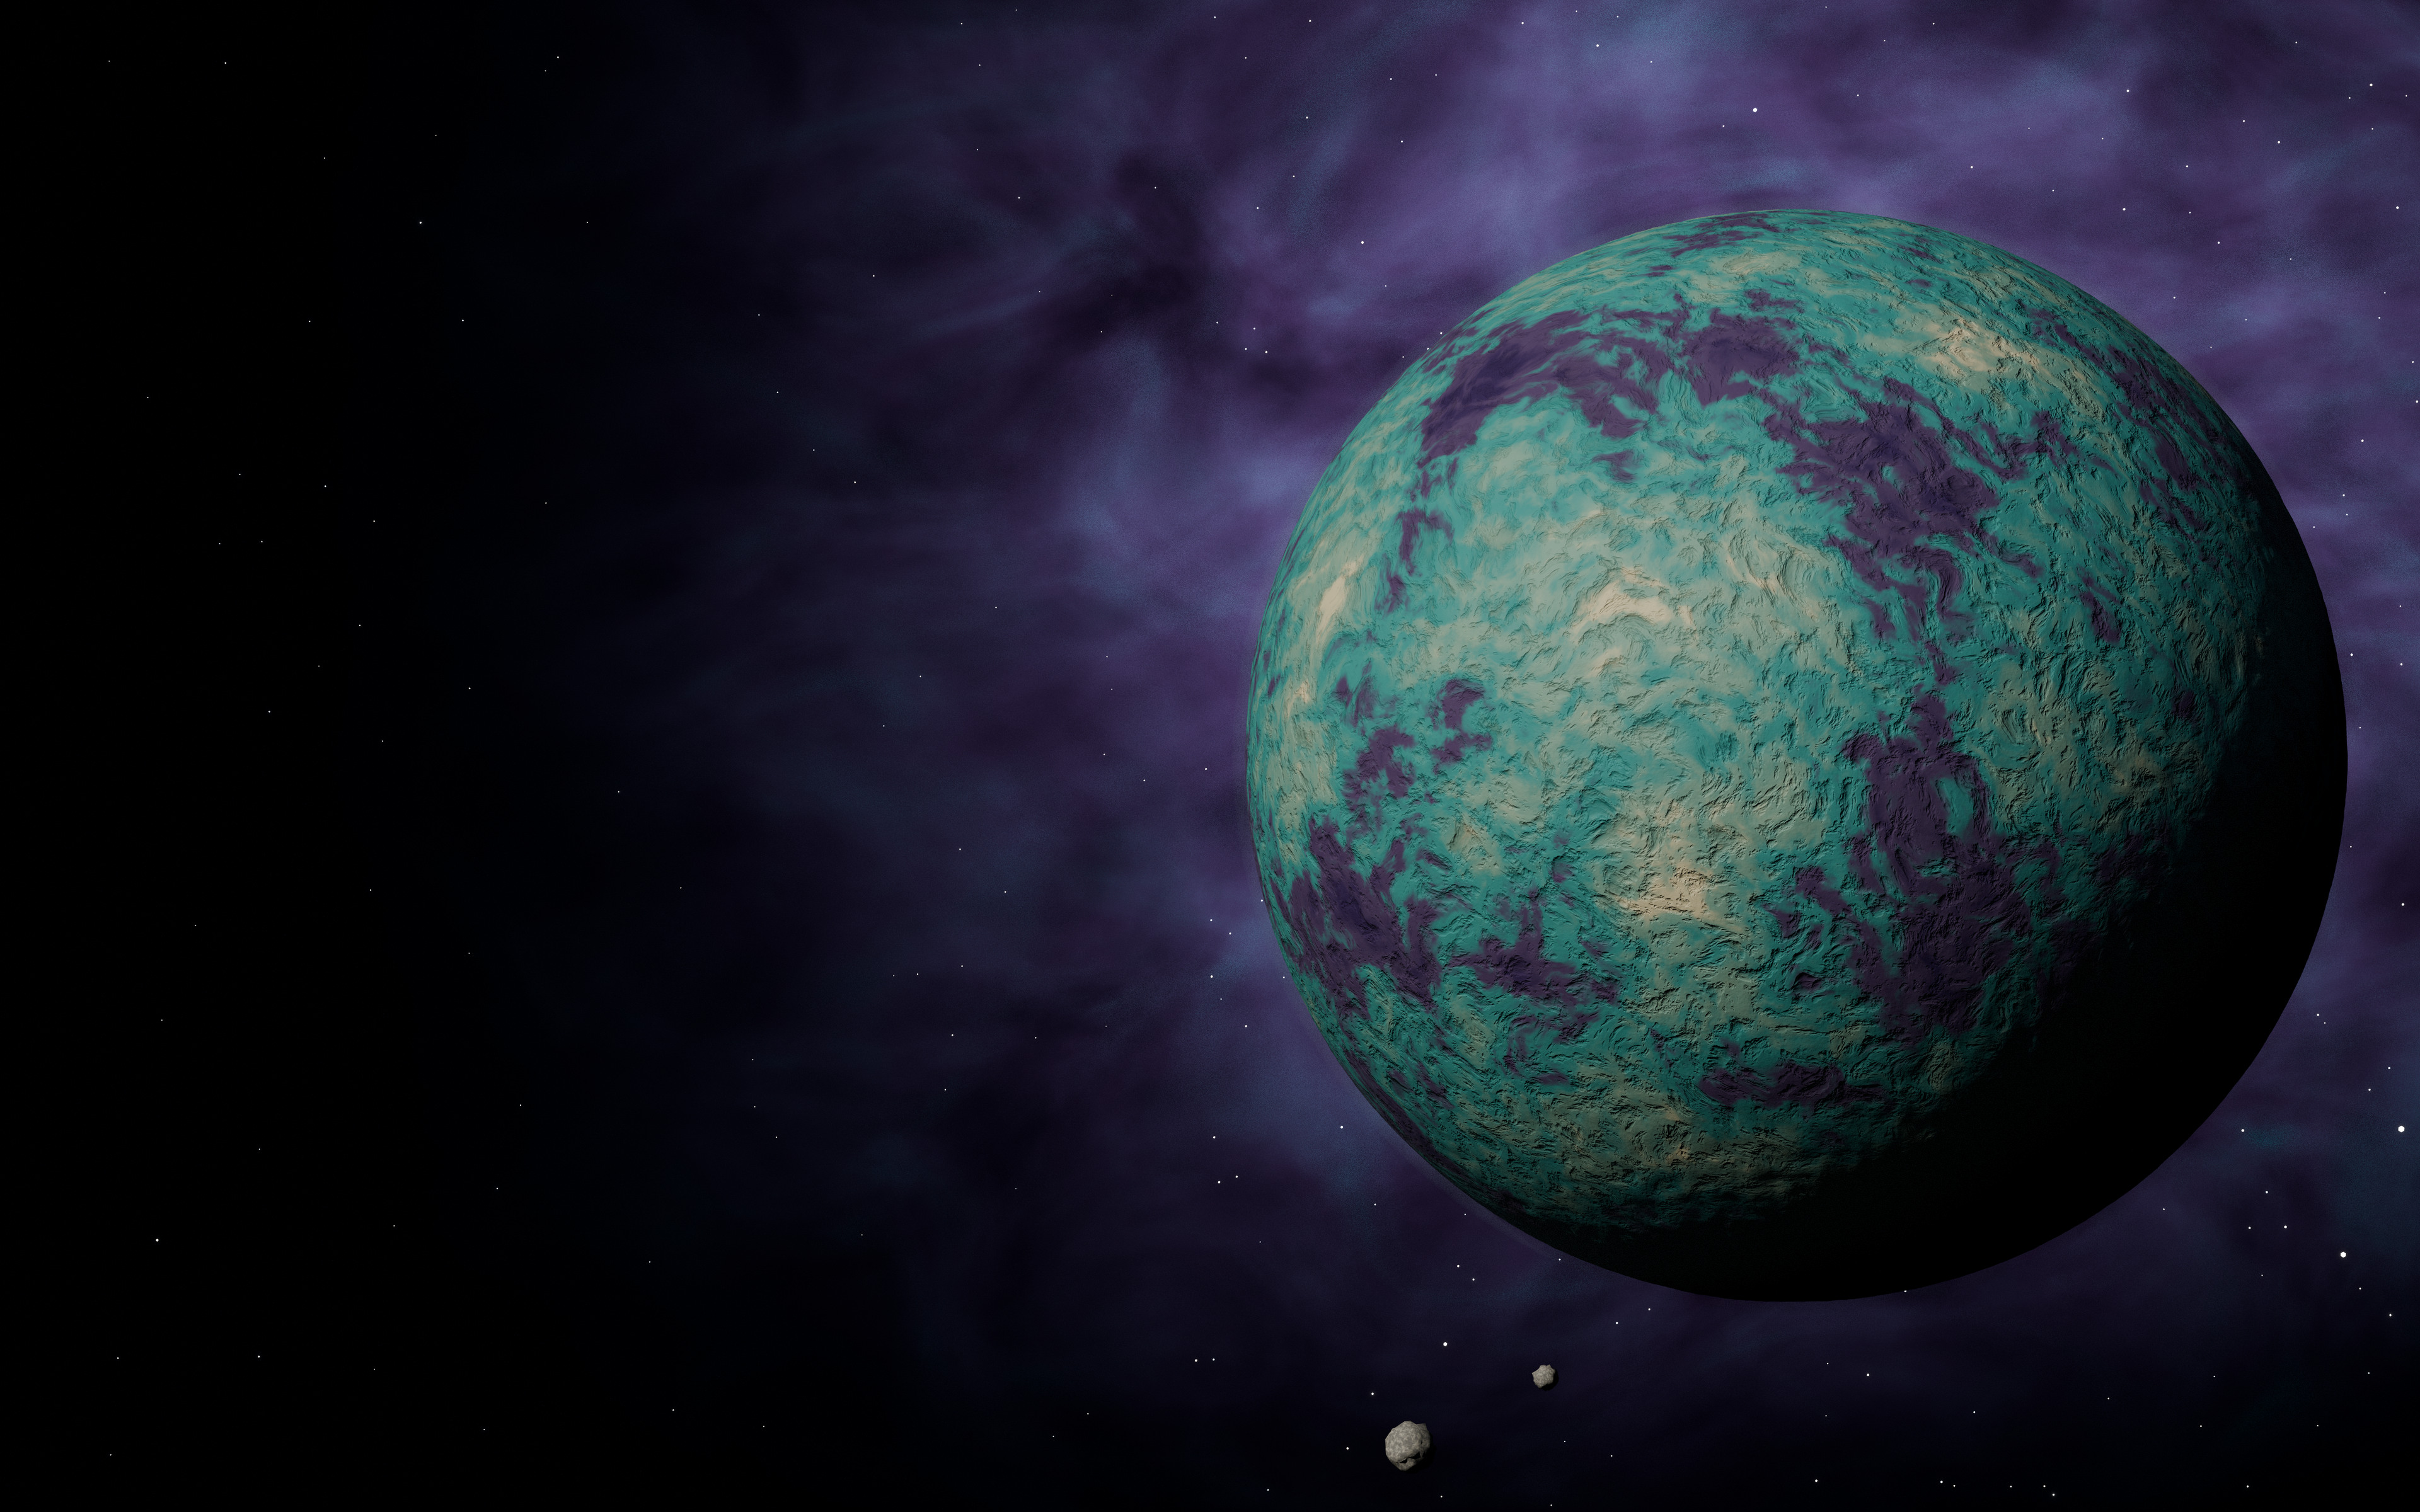
\includegraphics[width=\paperwidth,height=\paperheight]{Risorse/Copertine/M03_Iride.jpg}};

\node[anchor=north west,inner sep=0,text width=9.2cm] at
 ([xshift=1.05cm,yshift=-1.10cm]current page.north west)
 {\color{Mint}\bfseries\fontsize{23}{27}\selectfont IRIDE};
\node[anchor=north west,inner sep=0,text width=9.2cm] at
 ([xshift=1.07cm,yshift=-2.16cm]current page.north west)
 {\color{white}\fontsize{9.0}{12}\selectfont MODULO M03 · SCIENZE DELLA TERRA};
\draw[Mint,line width=1.4pt] ([xshift=1.05cm,yshift=-2.78cm]current page.north west)--
 ([xshift=2.60cm,yshift=-2.78cm]current page.north west);
\node[anchor=north west,inner sep=0] at
 ([xshift=1.05cm,yshift=-3.35cm]current page.north west)
 {\begin{minipage}{9.2cm}\raggedright\color{white}\bfseries
 \fontsize{30}{36}\selectfont Descrivere e\\visualizzare\\i dati\end{minipage}};
\node[anchor=north west,inner sep=0] at
 ([xshift=1.07cm,yshift=-7.88cm]current page.north west)
 {\begin{minipage}{9.0cm}\raggedright\color{Lilac}
 \fontsize{12.2}{17}\selectfont Distribuzioni, sintesi statistiche\\e rappresentazioni scientifiche\end{minipage}};
\node[anchor=north west,inner sep=0,text width=9.2cm] at
 ([xshift=1.07cm,yshift=-10.52cm]current page.north west)
 {\color{white}\fontsize{11.5}{15}\selectfont Marzio De Corato};
\node[anchor=north west,inner sep=0,text width=9.2cm] at
 ([xshift=1.07cm,yshift=-11.17cm]current page.north west)
 {\color{Lilac}\fontsize{8.8}{11}\selectfont \href{https://creativecommons.org/licenses/by-nc-sa/4.0/}{\textcopyright{} 2026 · CC BY-NC-SA 4.0}};
\end{tikzpicture}
\end{frame}


\begin{frame}[plain]\hypertarget{slide2}{}
\bookmark[level=0,page=2]{Domanda centrale}
\begin{tikzpicture}[remember picture,overlay]
\node[anchor=north west,inner sep=0] at ([xshift=.95cm,yshift=-.67cm]current page.north west) {\color{Navy}\bfseries\fontsize{23}{27}\selectfont Che cosa racconta una distribuzione?};
\draw[Classical,line width=1.4pt] ([xshift=.95cm,yshift=-1.73cm]current page.north west)--([xshift=2.5cm,yshift=-1.73cm]current page.north west);
\node[anchor=north west,inner sep=0,fill=GeoTint,rounded corners=2mm,text width=17.7cm,inner sep=3.5mm] at ([xshift=1.0cm,yshift=-2.26cm]current page.north west) {\color{Navy}\fontsize{14.1}{19}\selectfont Come riassumere i dati senza nasconderne variabilità e struttura?};
\node[draw=Rule,line width=.7pt,fill=GeoTint,rounded corners=2.5mm,minimum width=4.8cm,minimum height=2.15cm,text width=4.38cm,align=center,inner sep=3mm] (n0) at ([xshift=4cm,yshift=-6.15cm]current page.north west) {\color{Navy}\bfseries\fontsize{13}{16}\selectfont OSSERVAZIONI\\[2mm]\color{Ink}\normalfont\fontsize{10.5}{14}\selectfont Valori, unità e gruppi};
\node[draw=Rule,line width=.7pt,fill=Paper,rounded corners=2.5mm,minimum width=4.8cm,minimum height=2.15cm,text width=4.38cm,align=center,inner sep=3mm] (n1) at ([xshift=10cm,yshift=-6.15cm]current page.north west) {\color{Navy}\bfseries\fontsize{13}{16}\selectfont DISTRIBUZIONI\\[2mm]\color{Ink}\normalfont\fontsize{10.5}{14}\selectfont Forma, posizione\\e dispersione};
\node[draw=Rule,line width=.7pt,fill=GeoTint,rounded corners=2.5mm,minimum width=4.8cm,minimum height=2.15cm,text width=4.38cm,align=center,inner sep=3mm] (n2) at ([xshift=16cm,yshift=-6.15cm]current page.north west) {\color{Navy}\bfseries\fontsize{13}{16}\selectfont RELAZIONI\\[2mm]\color{Ink}\normalfont\fontsize{10.5}{14}\selectfont Confronti e associazioni};
\draw[-{Stealth[length=3.0mm]},draw=Classical,line width=1.45pt] ([xshift=6.65cm,yshift=-6.15cm]current page.north west)--([xshift=7.35cm,yshift=-6.15cm]current page.north west);
\draw[-{Stealth[length=3.0mm]},draw=Classical,line width=1.45pt] ([xshift=12.65cm,yshift=-6.15cm]current page.north west)--([xshift=13.35cm,yshift=-6.15cm]current page.north west);
\node[anchor=north west,inner sep=0,text width=17.9cm] at ([xshift=1.05cm,yshift=-8.25cm]current page.north west) {\color{Classical}\bfseries\fontsize{10.4}{13.4}\selectfont IDEA GUIDA};
\node[anchor=north west,inner sep=0,text width=17.85cm] at ([xshift=1.05cm,yshift=-8.71cm]current page.north west) {\color{Ink}\fontsize{11.9}{16.0}\selectfont Una figura e una statistica descrittiva rispondono a domande complementari: nessuna sintesi sostituisce il controllo dei dati.};
\draw[Rule,line width=.35pt] ([xshift=.95cm,yshift=-11.92cm]current page.north west)--([xshift=19.05cm,yshift=-11.92cm]current page.north west);
\node[anchor=north west,inner sep=0] at ([xshift=.95cm,yshift=-12.06cm]current page.north west) {\color{Muted}\fontsize{7.7}{9.3}\selectfont Iride · Descrivere e visualizzare i dati};
\node[anchor=north east,inner sep=0] at ([xshift=19.05cm,yshift=-12.06cm]current page.north west) {\color{Muted}\fontsize{7.7}{9.3}\selectfont 2/79};
\end{tikzpicture}
\end{frame}
\begin{frame}[plain]\hypertarget{slide3}{}
\bookmark[level=1,page=3]{Dalla tabella verificata alla descrizione}
\begin{tikzpicture}[remember picture,overlay]
\PilotChrome{Dalla tabella verificata alla descrizione}{DOMANDA E SUPPORTO}{3}{La domanda stabilisce quali variabili, unità di osservazione e confronti servono alla descrizione.}
\node[anchor=north west,inner sep=0] at ([xshift=0.96cm,yshift=-2.13cm]current page.north west) {\usebox{\PilotLeftBox}};
\node[anchor=north west,inner sep=0] at ([xshift=11.52cm,yshift=-2.13cm]current page.north west) {\usebox{\PilotRightBox}};

\end{tikzpicture}\end{frame}

% SLIDE 004 | Il caso principale: 160 fossili simulati
\begin{lrbox}{\PilotLeftBox}%
\begin{minipage}[t]{10.05cm}\raggedright\color{Ink}\fontsize{11.3}{14.8}\selectfont

\PLabel{Misure riferite al singolo individuo}
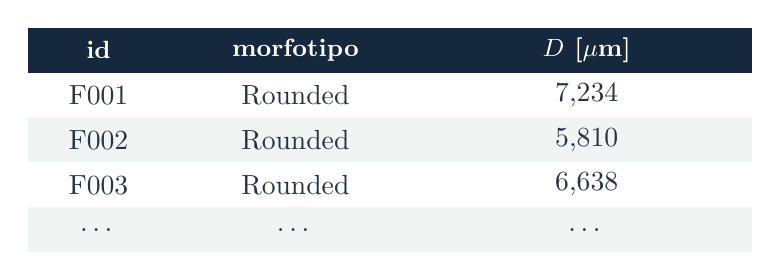
\begin{tikzpicture}[x=1cm,y=1cm]
\fill[Navy] (0,0) rectangle (9.200000000000001,0.57);
\node[font=\bfseries\fontsize{9.2}{11}\selectfont,text=white] at (0.9,0.285) {id};
\node[font=\bfseries\fontsize{9.2}{11}\selectfont,text=white] at (3.4000000000000004,0.285) {morfotipo};
\node[font=\bfseries\fontsize{9.2}{11}\selectfont,text=white] at (7.1,0.285) {$D$ [$\mu$m]};
\fill[white] (0,-0.57) rectangle (9.200000000000001,0.0);
\node[font=\fontsize{9.6}{12}\selectfont,text=Ink] at (0.9,-0.285) {F001};
\node[font=\fontsize{9.6}{12}\selectfont,text=Ink] at (3.4000000000000004,-0.285) {Rounded};
\node[font=\fontsize{9.6}{12}\selectfont,text=Ink] at (7.1,-0.285) {7,234};
\fill[GeoTint] (0,-1.14) rectangle (9.200000000000001,-0.57);
\node[font=\fontsize{9.6}{12}\selectfont,text=Ink] at (0.9,-0.855) {F002};
\node[font=\fontsize{9.6}{12}\selectfont,text=Ink] at (3.4000000000000004,-0.855) {Rounded};
\node[font=\fontsize{9.6}{12}\selectfont,text=Ink] at (7.1,-0.855) {5,810};
\fill[white] (0,-1.71) rectangle (9.200000000000001,-1.1400000000000001);
\node[font=\fontsize{9.6}{12}\selectfont,text=Ink] at (0.9,-1.425) {F003};
\node[font=\fontsize{9.6}{12}\selectfont,text=Ink] at (3.4000000000000004,-1.425) {Rounded};
\node[font=\fontsize{9.6}{12}\selectfont,text=Ink] at (7.1,-1.425) {6,638};
\fill[GeoTint] (0,-2.28) rectangle (9.200000000000001,-1.71);
\node[font=\fontsize{9.6}{12}\selectfont,text=Ink] at (0.9,-1.9949999999999999) {\dots};
\node[font=\fontsize{9.6}{12}\selectfont,text=Ink] at (3.4000000000000004,-1.9949999999999999) {\dots};
\node[font=\fontsize{9.6}{12}\selectfont,text=Ink] at (7.1,-1.9949999999999999) {\dots};
\end{tikzpicture}
\vspace{3mm}
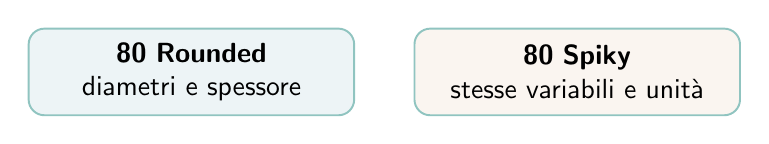
\begin{tikzpicture}[x=1cm,y=1cm]
\node[pFlow,text width=3.9cm,fill=GeoA!8] (a) at(2.2,.4){\textbf{80 Rounded}\\diametri e spessore};
\node[pFlow,text width=3.9cm,fill=GeoB!8] (b) at(7.1,.4){\textbf{80 Spiky}\\stesse variabili e unità};
\end{tikzpicture}
\PSmall{$D$ indica il diametro totale. I valori della tabella sono arrotondati solo per la lettura; il CSV conserva le cifre originali.}

\end{minipage}% 
\end{lrbox}
\typeout{FULLBOX:004:L:\the\ht\PilotLeftBox:\the\dp\PilotLeftBox}
\begin{lrbox}{\PilotRightBox}%
\begin{minipage}[t]{7.55cm}\raggedright\color{Ink}\fontsize{11.3}{14.8}\selectfont

\PCode{R · verificare il campione}{04_campione.R}
\PBody{Le quote 80/80 derivano dalla costruzione del dataset. Non stimano la prevalenza dei morfotipi in una popolazione naturale.}
\PInfo{Questo file completo di 160 individui è distinto dalle 25 registrazioni con anomalie usate per la pulizia dei dati in Tellus.}

\end{minipage}% 
\end{lrbox}
\typeout{FULLBOX:004:R:\the\ht\PilotRightBox:\the\dp\PilotRightBox}
\begin{frame}[plain]\hypertarget{slide4}{}
\bookmark[level=1,page=4]{Il caso principale: 160 fossili simulati}
\begin{tikzpicture}[remember picture,overlay]
\PilotChrome{Il caso principale: 160 fossili simulati}{DOMANDA E SUPPORTO}{4}{Una proporzione nel dataset descrive il campione; la sua interpretazione dipende da come il campione è stato costruito.}
\node[anchor=north west,inner sep=0] at ([xshift=0.96cm,yshift=-2.13cm]current page.north west) {\usebox{\PilotLeftBox}};
\node[anchor=north west,inner sep=0] at ([xshift=11.52cm,yshift=-2.13cm]current page.north west) {\usebox{\PilotRightBox}};

\end{tikzpicture}\end{frame}

% SLIDE 005 | Definire il campione prima del riepilogo
\begin{lrbox}{\PilotLeftBox}%
\begin{minipage}[t]{10.05cm}\raggedright\color{Ink}\fontsize{11.3}{14.8}\selectfont

\PLabel{Le condizioni di una descrizione confrontabile}
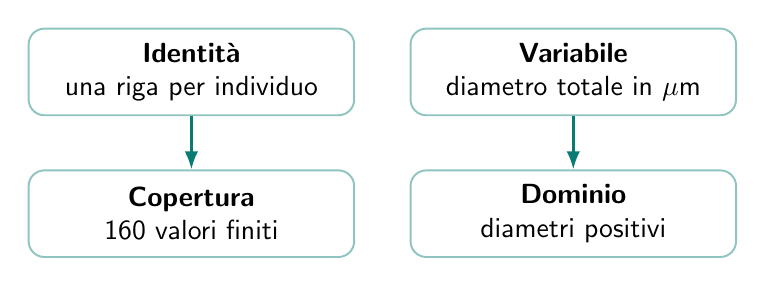
\begin{tikzpicture}[x=1cm,y=1cm]
\node[pFlow,text width=3.9cm] (a) at(2.2,3.1){\textbf{Identità}\\una riga per individuo};
\node[pFlow,text width=3.9cm] (b) at(7.05,3.1){\textbf{Variabile}\\diametro totale in $\mu$m};
\node[pFlow,text width=3.9cm] (c) at(2.2,1.3){\textbf{Copertura}\\160 valori finiti};
\node[pFlow,text width=3.9cm] (d) at(7.05,1.3){\textbf{Dominio}\\diametri positivi};
\draw[pEdge](a)--(c);\draw[pEdge](b)--(d);
\end{tikzpicture}
\PBody{Un controllo computazionale verifica una condizione dichiarata. Identificativi unici e valori positivi non dimostrano, da soli, la validità delle misure.}

\end{minipage}% 
\end{lrbox}
\typeout{FULLBOX:005:L:\the\ht\PilotLeftBox:\the\dp\PilotLeftBox}
\begin{lrbox}{\PilotRightBox}%
\begin{minipage}[t]{7.55cm}\raggedright\color{Ink}\fontsize{11.3}{14.8}\selectfont

\PCode{R · condizioni esplicite}{05_controlli.R}
\PSmall{\texttt{is.finite()} esclude \texttt{NA}, \texttt{NaN} e valori infiniti. La condizione $D>0$ deriva dal significato fisico della misura.}
\PInfo{Se un controllo fallisce, documentare il problema prima di modificare il campione. Le esclusioni cambiano ciò che viene descritto.}

\end{minipage}% 
\end{lrbox}
\typeout{FULLBOX:005:R:\the\ht\PilotRightBox:\the\dp\PilotRightBox}
\begin{frame}[plain]\hypertarget{slide5}{}
\bookmark[level=1,page=5]{Definire il campione prima del riepilogo}
\begin{tikzpicture}[remember picture,overlay]
\PilotChrome{Definire il campione prima del riepilogo}{DOMANDA E SUPPORTO}{5}{Ogni sintesi deve riferirsi a una variabile, a un insieme di osservazioni e a criteri di inclusione dichiarati.}
\node[anchor=north west,inner sep=0] at ([xshift=0.96cm,yshift=-2.13cm]current page.north west) {\usebox{\PilotLeftBox}};
\node[anchor=north west,inner sep=0] at ([xshift=11.52cm,yshift=-2.13cm]current page.north west) {\usebox{\PilotRightBox}};

\end{tikzpicture}\end{frame}

% SLIDE 006 | Misure individuali e medie di stazione
\begin{lrbox}{\PilotLeftBox}%
\begin{minipage}[t]{10.05cm}\raggedright\color{Ink}\fontsize{11.3}{14.8}\selectfont

\PLabel{Cambiano le unità rappresentate}
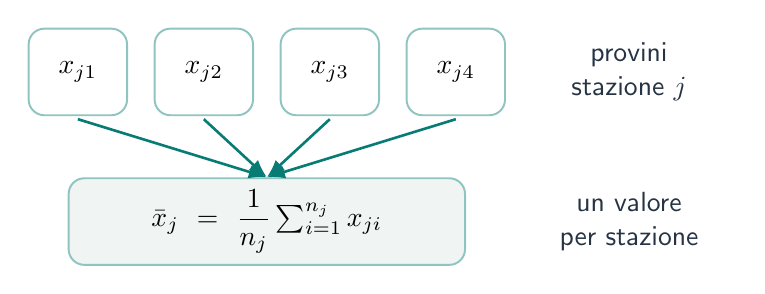
\begin{tikzpicture}[x=1cm,y=1cm]
\foreach \xx/\lab in {1.0/{x_{j1}},2.6/{x_{j2}},4.2/{x_{j3}},5.8/{x_{j4}}}{
  \node[pFlow,minimum width=1.25cm] at(\xx,3.1){$\lab$};}
\node[pFlow,text width=4.8cm,fill=GeoTint] (m) at(3.4,1.2){$\bar x_j=\dfrac{1}{n_j}\sum_{i=1}^{n_j}x_{ji}$};
\foreach \xx in {1.0,2.6,4.2,5.8}{\draw[pEdge](\xx,2.5)--(m.north);}
\node[pLabel,text width=2.5cm] at(8,3.1){provini\\stazione $j$};
\node[pLabel,text width=2.5cm] at(8,1.2){un valore\\per stazione};
\end{tikzpicture}
\PBody{Nei dati dei provini, ogni stazione comprende quattro misure. La distribuzione delle sei medie descrive le stazioni; la variabilità interna è stata riassunta.}

\end{minipage}% 
\end{lrbox}
\typeout{FULLBOX:006:L:\the\ht\PilotLeftBox:\the\dp\PilotLeftBox}
\begin{lrbox}{\PilotRightBox}%
\begin{minipage}[t]{7.55cm}\raggedright\color{Ink}\fontsize{11.3}{14.8}\selectfont

\PCode{R · cambiare il supporto}{06_supporto.R}
\PSmall{\texttt{aggregate()} separa le righe per stazione e applica \texttt{mean()} a ciascun gruppo. $n_j$ è il numero di provini della stazione $j$.}

\end{minipage}% 
\end{lrbox}
\typeout{FULLBOX:006:R:\the\ht\PilotRightBox:\the\dp\PilotRightBox}
\begin{frame}[plain]\hypertarget{slide6}{}
\bookmark[level=1,page=6]{Misure individuali e medie di stazione}
\begin{tikzpicture}[remember picture,overlay]
\PilotChrome{Misure individuali e medie di stazione}{DOMANDA E SUPPORTO}{6}{Il supporto indica a quale unità si riferisce il valore: individuo, stazione, intervallo o area.}
\node[anchor=north west,inner sep=0] at ([xshift=0.96cm,yshift=-2.13cm]current page.north west) {\usebox{\PilotLeftBox}};
\node[anchor=north west,inner sep=0] at ([xshift=11.52cm,yshift=-2.13cm]current page.north west) {\usebox{\PilotRightBox}};

\end{tikzpicture}\end{frame}

% SLIDE 007 | La stessa media può riassumere dati diversi
\begin{lrbox}{\PilotLeftBox}%
\begin{minipage}[t]{10.05cm}\raggedright\color{Ink}\fontsize{11.3}{14.8}\selectfont

\PLabel{Due campioni con centro uguale}
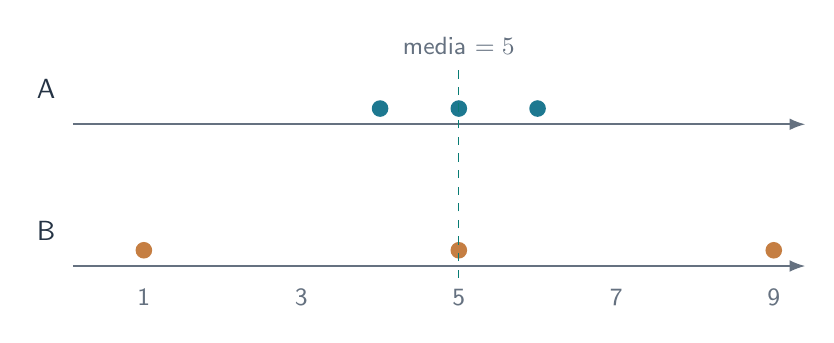
\begin{tikzpicture}[x=1cm,y=1cm]
\foreach \yy/\lab in {2.9/A,1.1/B}{
\draw[pAxis](.1,\yy)--(9.4,\yy);
\node[pLabel,anchor=east] at(.0,\yy+.45){\lab};}
\foreach \xx in {4,5,6}{\fill[GeoA](\xx,3.1) circle(3pt);}
\foreach \xx in {1,5,9}{\fill[GeoB](\xx,1.3) circle(3pt);}
\foreach \xx in {1,3,5,7,9}{\node[pNote] at(\xx,.7){\xx};}
\draw[Classical,dashed](5,.95)--(5,3.6);
\node[pNote] at(5,3.9){media $=5$};
\end{tikzpicture}
\PBody{Entrambi i campioni hanno $n=3$ e media 5. Gli scarti dalla media e la dispersione sono diversi.}
\PInfo{Una sintesi riduce le informazioni disponibili. Per valutare la dispersione, occorrono anche misure e grafici dedicati.}

\end{minipage}% 
\end{lrbox}
\typeout{FULLBOX:007:L:\the\ht\PilotLeftBox:\the\dp\PilotLeftBox}
\begin{lrbox}{\PilotRightBox}%
\begin{minipage}[t]{7.55cm}\raggedright\color{Ink}\fontsize{11.3}{14.8}\selectfont

\PCode{R · un controesempio minimo}{07_sintesi.R}
\PBody{\texttt{var()} calcola la varianza campionaria: somma degli scarti quadratici divisa per $n-1$. La riprenderemo nel blocco sulla dispersione.}

\end{minipage}% 
\end{lrbox}
\typeout{FULLBOX:007:R:\the\ht\PilotRightBox:\the\dp\PilotRightBox}
\begin{frame}[plain]\hypertarget{slide7}{}
\bookmark[level=1,page=7]{La stessa media può riassumere dati diversi}
\begin{tikzpicture}[remember picture,overlay]
\PilotChrome{La stessa media può riassumere dati diversi}{DOMANDA E SUPPORTO}{7}{La coincidenza di una statistica non implica che coincidano le distribuzioni dei dati.}
\node[anchor=north west,inner sep=0] at ([xshift=0.96cm,yshift=-2.13cm]current page.north west) {\usebox{\PilotLeftBox}};
\node[anchor=north west,inner sep=0] at ([xshift=11.52cm,yshift=-2.13cm]current page.north west) {\usebox{\PilotRightBox}};

\end{tikzpicture}\end{frame}

% SLIDE 008 | Scegliere la figura a partire dalla domanda
\begin{lrbox}{\PilotLeftBox}%
\begin{minipage}[t]{10.05cm}\raggedright\color{Ink}\fontsize{11.3}{14.8}\selectfont

\PLabel{Variabili e unità guidano la scelta}
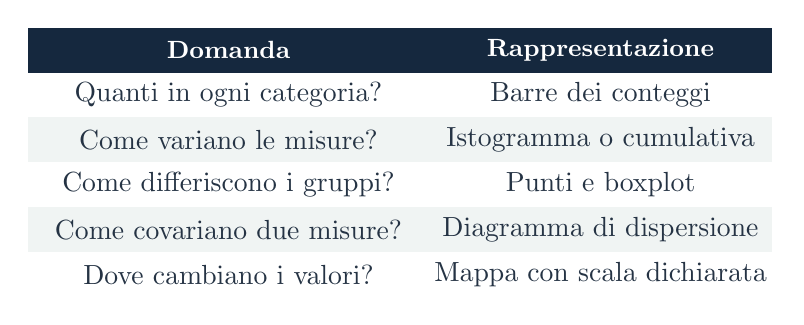
\begin{tikzpicture}[x=1cm,y=1cm]
\fill[Navy] (0,0) rectangle (9.45,0.57);
\node[font=\bfseries\fontsize{9.2}{11}\selectfont,text=white] at (2.55,0.285) {Domanda};
\node[font=\bfseries\fontsize{9.2}{11}\selectfont,text=white] at (7.2749999999999995,0.285) {Rappresentazione};
\fill[white] (0,-0.57) rectangle (9.45,0.0);
\node[font=\fontsize{9.6}{12}\selectfont,text=Ink] at (2.55,-0.285) {Quanti in ogni categoria?};
\node[font=\fontsize{9.6}{12}\selectfont,text=Ink] at (7.2749999999999995,-0.285) {Barre dei conteggi};
\fill[GeoTint] (0,-1.14) rectangle (9.45,-0.57);
\node[font=\fontsize{9.6}{12}\selectfont,text=Ink] at (2.55,-0.855) {Come variano le misure?};
\node[font=\fontsize{9.6}{12}\selectfont,text=Ink] at (7.2749999999999995,-0.855) {Istogramma o cumulativa};
\fill[white] (0,-1.71) rectangle (9.45,-1.1400000000000001);
\node[font=\fontsize{9.6}{12}\selectfont,text=Ink] at (2.55,-1.425) {Come differiscono i gruppi?};
\node[font=\fontsize{9.6}{12}\selectfont,text=Ink] at (7.2749999999999995,-1.425) {Punti e boxplot};
\fill[GeoTint] (0,-2.28) rectangle (9.45,-1.71);
\node[font=\fontsize{9.6}{12}\selectfont,text=Ink] at (2.55,-1.9949999999999999) {Come covariano due misure?};
\node[font=\fontsize{9.6}{12}\selectfont,text=Ink] at (7.2749999999999995,-1.9949999999999999) {Diagramma di dispersione};
\fill[white] (0,-2.8499999999999996) rectangle (9.45,-2.28);
\node[font=\fontsize{9.6}{12}\selectfont,text=Ink] at (2.55,-2.5649999999999995) {Dove cambiano i valori?};
\node[font=\fontsize{9.6}{12}\selectfont,text=Ink] at (7.2749999999999995,-2.5649999999999995) {Mappa con scala dichiarata};
\end{tikzpicture}
\vspace{3mm}\PBody{Le figure rispondono a domande specifiche. Le stesse osservazioni possono richiedere più rappresentazioni complementari.}

\end{minipage}% 
\end{lrbox}
\typeout{FULLBOX:008:L:\the\ht\PilotLeftBox:\the\dp\PilotLeftBox}
\begin{lrbox}{\PilotRightBox}%
\begin{minipage}[t]{7.55cm}\raggedright\color{Ink}\fontsize{11.3}{14.8}\selectfont

\PLabel{Prima di disegnare}
\PBody{Scrivere una frase che specifichi la quantità da descrivere, il campione e il confronto.}
\vspace{3mm}\PInfo{Esempio: «Confrontare la distribuzione del diametro totale, in micrometri, negli 80 Rounded e negli 80 Spiky simulati».}
\vspace{2mm}\PSmall{La frase stabilisce variabile, unità, gruppi e numerosità. Posizione e dispersione verranno esaminate insieme.}

\end{minipage}% 
\end{lrbox}
\typeout{FULLBOX:008:R:\the\ht\PilotRightBox:\the\dp\PilotRightBox}
\begin{frame}[plain]\hypertarget{slide8}{}
\bookmark[level=1,page=8]{Scegliere la figura a partire dalla domanda}
\begin{tikzpicture}[remember picture,overlay]
\PilotChrome{Scegliere la figura a partire dalla domanda}{DOMANDA E SUPPORTO}{8}{Una figura è adeguata quando rende leggibile il carattere dei dati che la domanda richiede di esaminare.}
\node[anchor=north west,inner sep=0] at ([xshift=0.96cm,yshift=-2.13cm]current page.north west) {\usebox{\PilotLeftBox}};
\node[anchor=north west,inner sep=0] at ([xshift=11.52cm,yshift=-2.13cm]current page.north west) {\usebox{\PilotRightBox}};

\end{tikzpicture}\end{frame}

% SLIDE 009 | Laboratorio: che cosa rappresenta un punto?
\begin{lrbox}{\PilotLeftBox}%
\begin{minipage}[t]{10.05cm}\raggedright\color{Ink}\fontsize{11.3}{14.8}\selectfont

\PLabel{Esperimento m03-supporto}
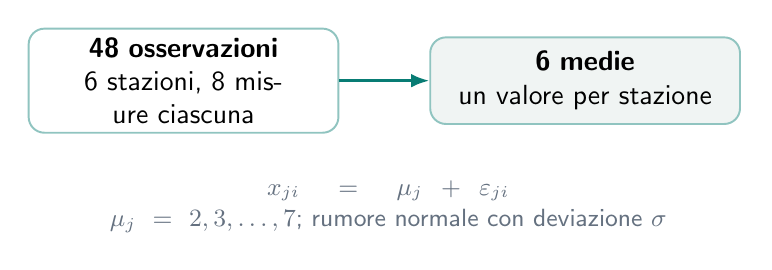
\begin{tikzpicture}[x=1cm,y=1cm]
\node[pFlow,text width=3.7cm] (a) at(2.1,2.7){\textbf{48 osservazioni}\\6 stazioni, 8 misure ciascuna};
\node[pFlow,text width=3.7cm,fill=GeoTint] (b) at(7.2,2.7){\textbf{6 medie}\\un valore per stazione};
\draw[pEdge](a)--(b);
\node[pNote,text width=8.8cm] at(4.7,1.1){$x_{ji}=\mu_j+\varepsilon_{ji}$\\$\mu_j=2,3,\ldots,7$; rumore normale con deviazione $\sigma$};
\end{tikzpicture}
\PBody{Confrontare $\sigma=1$ e $\sigma=3$, conservando il seme 17. Indicare quali informazioni sono visibili nei punti e quali nelle medie.}
\PSmall{\href{https://marzione00.github.io/Lab_Geo/\#laboratorio/m03-supporto}{Apri l'esperimento · Supporto della rappresentazione}}

\end{minipage}% 
\end{lrbox}
\typeout{FULLBOX:009:L:\the\ht\PilotLeftBox:\the\dp\PilotLeftBox}
\begin{lrbox}{\PilotRightBox}%
\begin{minipage}[t]{7.55cm}\raggedright\color{Ink}\fontsize{11.3}{14.8}\selectfont

\PCode{R · due scenari riproducibili}{09_lab_supporto.R}
\PBody{Nel quaderno riportare numerosità, supporto e un'osservazione sulla variabilità interna. Le medie osservate risentono anche del rumore.}
\PSmall{La funzione restituisce \texttt{dati}, \texttt{medie} e \texttt{indicatori}. Il codice completo è distribuito nel progetto.}

\end{minipage}% 
\end{lrbox}
\typeout{FULLBOX:009:R:\the\ht\PilotRightBox:\the\dp\PilotRightBox}
\begin{frame}[plain]\hypertarget{slide9}{}
\bookmark[level=1,page=9]{Laboratorio: che cosa rappresenta un punto?}
\begin{tikzpicture}[remember picture,overlay]
\PilotChrome{Laboratorio: che cosa rappresenta un punto?}{LABORATORIO · SUPPORTO}{9}{Confrontare una nuvola di misure con le medie richiede di dichiarare che cosa rappresenta ciascun punto.}
\node[anchor=north west,inner sep=0] at ([xshift=0.96cm,yshift=-2.13cm]current page.north west) {\usebox{\PilotLeftBox}};
\node[anchor=north west,inner sep=0] at ([xshift=11.52cm,yshift=-2.13cm]current page.north west) {\usebox{\PilotRightBox}};

\end{tikzpicture}\end{frame}

% SLIDE 010 | Frequenze assolute: contare le unità
\begin{lrbox}{\PilotLeftBox}%
\begin{minipage}[t]{10.05cm}\raggedright\color{Ink}\fontsize{11.3}{14.8}\selectfont

\PLabel{Una variabile categoriale}
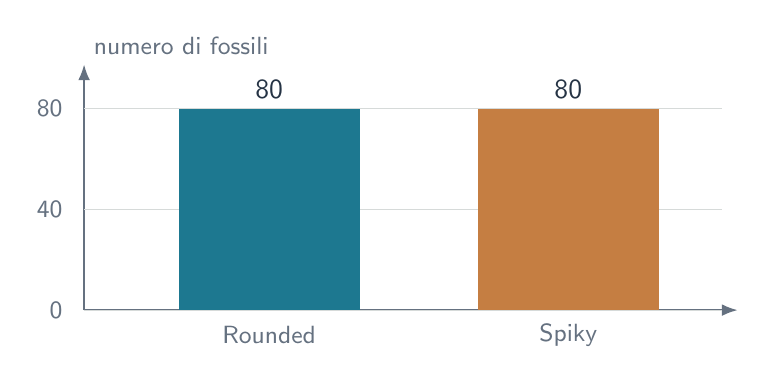
\begin{tikzpicture}[x=1cm,y=.8cm]
\draw[pAxis](1,0)--(1,3.9);\draw[pAxis](1,0)--(9.3,0);
\foreach \y/\lab in {0/0,1.6/40,3.2/80}{\draw[Rule](1,\y)--(9.1,\y);\node[pNote,anchor=east] at(.85,\y){\lab};}
\fill[GeoA](2.2,0)rectangle(4.5,3.2);\fill[GeoB](6,0)rectangle(8.3,3.2);
\node[pLabel] at(3.35,3.5){80};\node[pLabel] at(7.15,3.5){80};
\node[pNote] at(3.35,-.4){Rounded};\node[pNote] at(7.15,-.4){Spiky};
\node[pNote,anchor=west] at(1,4.2){numero di fossili};
\end{tikzpicture}
\[n_k=\sum_{i=1}^{n}\mathbf{1}(g_i=k),\qquad \sum_k n_k=n.\]
\PSmall{$g_i$ è la categoria dell'individuo $i$; l'indicatrice vale 1 se $g_i=k$, altrimenti 0. Le categorie sono esaustive e mutuamente esclusive.}

\end{minipage}% 
\end{lrbox}
\typeout{FULLBOX:010:L:\the\ht\PilotLeftBox:\the\dp\PilotLeftBox}
\begin{lrbox}{\PilotRightBox}%
\begin{minipage}[t]{7.55cm}\raggedright\color{Ink}\fontsize{11.3}{14.8}\selectfont

\PCode{R · contare e rappresentare}{10_conteggi.R}
\PBody{\texttt{table()} associa ogni categoria al numero di osservazioni. \texttt{barplot()} disegna una barra per categoria.}
\PSmall{Lo zero costituisce la base della scala. La larghezza delle barre non rappresenta un intervallo numerico.}

\end{minipage}% 
\end{lrbox}
\typeout{FULLBOX:010:R:\the\ht\PilotRightBox:\the\dp\PilotRightBox}
\begin{frame}[plain]\hypertarget{slide10}{}
\bookmark[level=1,page=10]{Frequenze assolute: contare le unità}
\begin{tikzpicture}[remember picture,overlay]
\PilotChrome{Frequenze assolute: contare le unità}{FREQUENZE E DENOMINATORI}{10}{La frequenza assoluta conta quante unità appartengono a una categoria definita.}
\node[anchor=north west,inner sep=0] at ([xshift=0.96cm,yshift=-2.13cm]current page.north west) {\usebox{\PilotLeftBox}};
\node[anchor=north west,inner sep=0] at ([xshift=11.52cm,yshift=-2.13cm]current page.north west) {\usebox{\PilotRightBox}};

\end{tikzpicture}\end{frame}

% SLIDE 011 | Proporzioni e percentuali
\begin{lrbox}{\PilotLeftBox}%
\begin{minipage}[t]{10.05cm}\raggedright\color{Ink}\fontsize{11.3}{14.8}\selectfont

\PLabel{Rapportare il conteggio al totale pertinente}
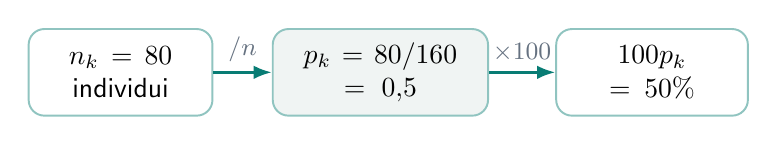
\begin{tikzpicture}[x=1cm,y=1cm]
\node[pFlow,text width=2.1cm] (n) at(1.25,2.2){$n_k=80$\\individui};
\node[pFlow,text width=2.5cm,fill=GeoTint] (p) at(4.55,2.2){$p_k=80/160$\\$=0{,}5$};
\node[pFlow,text width=2.2cm] (q) at(8,2.2){$100p_k$\\$=50\%$};
\draw[pEdge](n)--node[above,pNote]{$/n$}(p);
\draw[pEdge](p)--node[above,pNote]{$\times100$}(q);
\end{tikzpicture}
\[p_k=\frac{n_k}{n},\qquad 0\le p_k\le1,\qquad \sum_k p_k=1.\]
\PBody{Una proporzione è adimensionale. Il denominatore deve contenere tutte le unità a cui il confronto si riferisce.}

\end{minipage}% 
\end{lrbox}
\typeout{FULLBOX:011:L:\the\ht\PilotLeftBox:\the\dp\PilotLeftBox}
\begin{lrbox}{\PilotRightBox}%
\begin{minipage}[t]{7.55cm}\raggedright\color{Ink}\fontsize{11.3}{14.8}\selectfont

\PCode{R · dal conteggio alla proporzione}{11_proporzioni.R}
\PBody{\texttt{prop.table()} divide ogni cella per il totale scelto. Senza indicare un margine, usa il totale dell'intera tabella.}
\PInfo{«50\%» è una descrizione incompleta senza specificare il gruppo, la variabile e il totale da cui deriva.}

\end{minipage}% 
\end{lrbox}
\typeout{FULLBOX:011:R:\the\ht\PilotRightBox:\the\dp\PilotRightBox}
\begin{frame}[plain]\hypertarget{slide11}{}
\bookmark[level=1,page=11]{Proporzioni e percentuali}
\begin{tikzpicture}[remember picture,overlay]
\PilotChrome{Proporzioni e percentuali}{FREQUENZE E DENOMINATORI}{11}{Un conteggio e una percentuale descrivono aspetti diversi: numerosità e composizione dell’insieme scelto.}
\node[anchor=north west,inner sep=0] at ([xshift=0.96cm,yshift=-2.13cm]current page.north west) {\usebox{\PilotLeftBox}};
\node[anchor=north west,inner sep=0] at ([xshift=11.52cm,yshift=-2.13cm]current page.north west) {\usebox{\PilotRightBox}};

\end{tikzpicture}\end{frame}

% SLIDE 012 | Tabelle a doppia entrata e margini
\begin{lrbox}{\PilotLeftBox}%
\begin{minipage}[t]{10.05cm}\raggedright\color{Ink}\fontsize{11.3}{14.8}\selectfont

\PLabel{Ogni denominatore risponde a una domanda}
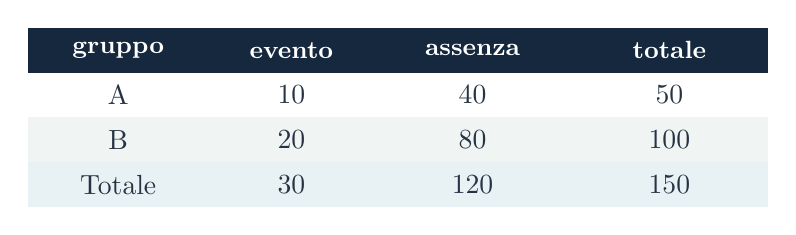
\begin{tikzpicture}[x=1cm,y=1cm]
\fill[Navy] (0,0) rectangle (9.4,0.57);
\node[font=\bfseries\fontsize{9.2}{11}\selectfont,text=white] at (1.15,0.285) {gruppo};
\node[font=\bfseries\fontsize{9.2}{11}\selectfont,text=white] at (3.3499999999999996,0.285) {evento};
\node[font=\bfseries\fontsize{9.2}{11}\selectfont,text=white] at (5.65,0.285) {assenza};
\node[font=\bfseries\fontsize{9.2}{11}\selectfont,text=white] at (8.15,0.285) {totale};
\fill[white] (0,-0.57) rectangle (9.4,0.0);
\node[font=\fontsize{9.6}{12}\selectfont,text=Ink] at (1.15,-0.285) {A};
\node[font=\fontsize{9.6}{12}\selectfont,text=Ink] at (3.3499999999999996,-0.285) {10};
\node[font=\fontsize{9.6}{12}\selectfont,text=Ink] at (5.65,-0.285) {40};
\node[font=\fontsize{9.6}{12}\selectfont,text=Ink] at (8.15,-0.285) {50};
\fill[GeoTint] (0,-1.14) rectangle (9.4,-0.57);
\node[font=\fontsize{9.6}{12}\selectfont,text=Ink] at (1.15,-0.855) {B};
\node[font=\fontsize{9.6}{12}\selectfont,text=Ink] at (3.3499999999999996,-0.855) {20};
\node[font=\fontsize{9.6}{12}\selectfont,text=Ink] at (5.65,-0.855) {80};
\node[font=\fontsize{9.6}{12}\selectfont,text=Ink] at (8.15,-0.855) {100};
\fill[GeoA!10] (0,-1.71) rectangle (9.4,-1.1400000000000001);
\node[font=\fontsize{9.6}{12}\selectfont,text=Ink] at (1.15,-1.425) {Totale};
\node[font=\fontsize{9.6}{12}\selectfont,text=Ink] at (3.3499999999999996,-1.425) {30};
\node[font=\fontsize{9.6}{12}\selectfont,text=Ink] at (5.65,-1.425) {120};
\node[font=\fontsize{9.6}{12}\selectfont,text=Ink] at (8.15,-1.425) {150};
\end{tikzpicture}
\vspace{3mm}
\[p_{k\mid j}=\frac{n_{jk}}{\sum_k n_{jk}}.\]
\PBody{Fra gli individui di A, la quota con evento è $10/50=20\%$. Fra tutti gli eventi, la quota proveniente da A è $10/30\simeq33{,}3\%$.}
\PSmall{$j$ identifica il gruppo; $k$ l'esito. L'esempio è costruito per distinguere i due condizionamenti.}

\end{minipage}% 
\end{lrbox}
\typeout{FULLBOX:012:L:\the\ht\PilotLeftBox:\the\dp\PilotLeftBox}
\begin{lrbox}{\PilotRightBox}%
\begin{minipage}[t]{7.55cm}\raggedright\color{Ink}\fontsize{11.3}{14.8}\selectfont

\PCode{R · normalizzare lungo un margine}{12_doppia_entrata.R}
\PSmall{\texttt{margin = 1} divide per i totali di riga. \texttt{margin = 2} divide per i totali di colonna. Le celle sono le stesse; cambia la domanda.}

\end{minipage}% 
\end{lrbox}
\typeout{FULLBOX:012:R:\the\ht\PilotRightBox:\the\dp\PilotRightBox}
\begin{frame}[plain]\hypertarget{slide12}{}
\bookmark[level=1,page=12]{Tabelle a doppia entrata e margini}
\begin{tikzpicture}[remember picture,overlay]
\PilotChrome{Tabelle a doppia entrata e margini}{FREQUENZE E DENOMINATORI}{12}{Prima di confrontare percentuali, controllare a quali totali sono rapportati i conteggi.}
\node[anchor=north west,inner sep=0] at ([xshift=0.96cm,yshift=-2.13cm]current page.north west) {\usebox{\PilotLeftBox}};
\node[anchor=north west,inner sep=0] at ([xshift=11.52cm,yshift=-2.13cm]current page.north west) {\usebox{\PilotRightBox}};

\end{tikzpicture}\end{frame}

% SLIDE 013 | Dati mancanti: quota osservata e copertura
\begin{lrbox}{\PilotLeftBox}%
\begin{minipage}[t]{10.05cm}\raggedright\color{Ink}\fontsize{11.3}{14.8}\selectfont

\PLabel{Un esempio di sei unità previste}
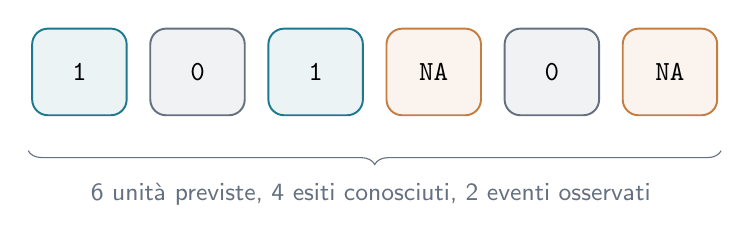
\begin{tikzpicture}[x=1cm,y=1cm]
\foreach \xx/\v/\col in {0.8/1/GeoA,2.3/0/Muted,3.8/1/GeoA,5.3/NA/GeoB,6.8/0/Muted,8.3/NA/GeoB}{
\node[pFlow,minimum width=1.2cm,draw=\col,fill=\col!9] at(\xx,2.8){\texttt{\v}};}
\draw[decorate,decoration={brace,amplitude=5pt},Muted](8.95,1.8)--(.15,1.8);
\node[pNote] at(4.5,1.25){6 unità previste, 4 esiti conosciuti, 2 eventi osservati};
\end{tikzpicture}
\[p_{\mathrm{validi}}=\frac{2}{4}=0{,}50,
\qquad c=\frac{4}{6}\simeq0{,}667.\]
\PBody{I valori mancanti non attestano l'assenza dell'evento. Il 50\% descrive gli esiti conosciuti; la copertura è circa 66,7\%.}

\end{minipage}% 
\end{lrbox}
\typeout{FULLBOX:013:L:\the\ht\PilotLeftBox:\the\dp\PilotLeftBox}
\begin{lrbox}{\PilotRightBox}%
\begin{minipage}[t]{7.55cm}\raggedright\color{Ink}\fontsize{11.3}{14.8}\selectfont

\PCode{R · dichiarare due denominatori}{13_copertura.R}
\PSmall{\texttt{na.rm = TRUE} esclude gli ignoti dal conteggio. Non recupera le informazioni mancanti né rende rappresentativo il sottoinsieme osservato.}

\end{minipage}% 
\end{lrbox}
\typeout{FULLBOX:013:R:\the\ht\PilotRightBox:\the\dp\PilotRightBox}
\begin{frame}[plain]\hypertarget{slide13}{}
\bookmark[level=1,page=13]{Dati mancanti: quota osservata e copertura}
\begin{tikzpicture}[remember picture,overlay]
\PilotChrome{Dati mancanti: quota osservata e copertura}{FREQUENZE E DENOMINATORI}{13}{Riportare insieme la quota tra i valori disponibili e quanti esiti erano effettivamente conosciuti.}
\node[anchor=north west,inner sep=0] at ([xshift=0.96cm,yshift=-2.13cm]current page.north west) {\usebox{\PilotLeftBox}};
\node[anchor=north west,inner sep=0] at ([xshift=11.52cm,yshift=-2.13cm]current page.north west) {\usebox{\PilotRightBox}};

\end{tikzpicture}\end{frame}

% SLIDE 014 | Pesi e media di gruppi
\begin{lrbox}{\PilotLeftBox}%
\begin{minipage}[t]{10.05cm}\raggedright\color{Ink}\fontsize{11.3}{14.8}\selectfont

\PLabel{Dare lo stesso peso ai gruppi oppure agli individui}
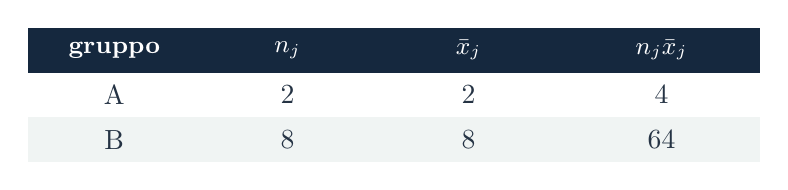
\begin{tikzpicture}[x=1cm,y=1cm]
\fill[Navy] (0,0) rectangle (9.3,0.57);
\node[font=\bfseries\fontsize{9.2}{11}\selectfont,text=white] at (1.1,0.285) {gruppo};
\node[font=\bfseries\fontsize{9.2}{11}\selectfont,text=white] at (3.3000000000000003,0.285) {$n_j$};
\node[font=\bfseries\fontsize{9.2}{11}\selectfont,text=white] at (5.6000000000000005,0.285) {$\bar x_j$};
\node[font=\bfseries\fontsize{9.2}{11}\selectfont,text=white] at (8.05,0.285) {$n_j\bar x_j$};
\fill[white] (0,-0.57) rectangle (9.3,0.0);
\node[font=\fontsize{9.6}{12}\selectfont,text=Ink] at (1.1,-0.285) {A};
\node[font=\fontsize{9.6}{12}\selectfont,text=Ink] at (3.3000000000000003,-0.285) {2};
\node[font=\fontsize{9.6}{12}\selectfont,text=Ink] at (5.6000000000000005,-0.285) {2};
\node[font=\fontsize{9.6}{12}\selectfont,text=Ink] at (8.05,-0.285) {4};
\fill[GeoTint] (0,-1.14) rectangle (9.3,-0.57);
\node[font=\fontsize{9.6}{12}\selectfont,text=Ink] at (1.1,-0.855) {B};
\node[font=\fontsize{9.6}{12}\selectfont,text=Ink] at (3.3000000000000003,-0.855) {8};
\node[font=\fontsize{9.6}{12}\selectfont,text=Ink] at (5.6000000000000005,-0.855) {8};
\node[font=\fontsize{9.6}{12}\selectfont,text=Ink] at (8.05,-0.855) {64};
\end{tikzpicture}
\vspace{3mm}
\[\bar x=\frac{\sum_j n_j\bar x_j}{\sum_j n_j}
      =\frac{4+64}{10}=6{,}8.\]
\PBody{La media non pesata delle due medie vale 5. La media degli individui vale 6,8: il gruppo B contiene otto osservazioni.}
\PSmall{Le due espressioni coincidono se i gruppi hanno uguale numerosità. Esempio costruito, adimensionale.}

\end{minipage}% 
\end{lrbox}
\typeout{FULLBOX:014:L:\the\ht\PilotLeftBox:\the\dp\PilotLeftBox}
\begin{lrbox}{\PilotRightBox}%
\begin{minipage}[t]{7.55cm}\raggedright\color{Ink}\fontsize{11.3}{14.8}\selectfont

\PCode{R · pesare per la numerosità}{14_pesi.R}
\PBody{Per pesi $w_j\ge0$ con somma positiva,}
\[\bar x_w=\frac{\sum_j w_j x_j}{\sum_j w_j}.\]
\PSmall{Il significato dei pesi dipende dalla domanda: numerosità, volume o probabilità di inclusione richiedono interpretazioni diverse.}

\end{minipage}% 
\end{lrbox}
\typeout{FULLBOX:014:R:\the\ht\PilotRightBox:\the\dp\PilotRightBox}
\begin{frame}[plain]\hypertarget{slide14}{}
\bookmark[level=1,page=14]{Pesi e media di gruppi}
\begin{tikzpicture}[remember picture,overlay]
\PilotChrome{Pesi e media di gruppi}{FREQUENZE E DENOMINATORI}{14}{La media di medie descrive gli individui solo quando i pesi rispettano la numerosità dei gruppi.}
\node[anchor=north west,inner sep=0] at ([xshift=0.96cm,yshift=-2.13cm]current page.north west) {\usebox{\PilotLeftBox}};
\node[anchor=north west,inner sep=0] at ([xshift=11.52cm,yshift=-2.13cm]current page.north west) {\usebox{\PilotRightBox}};

\end{tikzpicture}\end{frame}

% SLIDE 015 | Laboratorio: più eventi significa quota maggiore?
\begin{lrbox}{\PilotLeftBox}%
\begin{minipage}[t]{10.05cm}\raggedright\color{Ink}\fontsize{11.3}{14.8}\selectfont

\PLabel{Esperimento m03-denominatori}
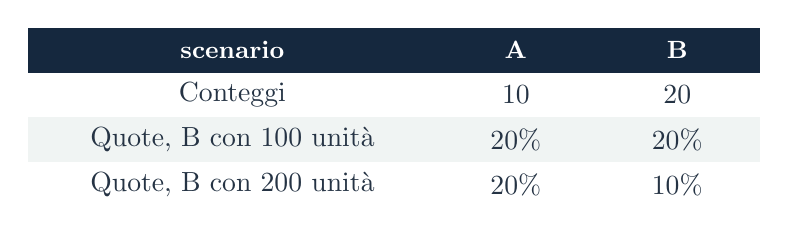
\begin{tikzpicture}[x=1cm,y=1cm]
\fill[Navy] (0,0) rectangle (9.3,0.57);
\node[font=\bfseries\fontsize{9.2}{11}\selectfont,text=white] at (2.6,0.285) {scenario};
\node[font=\bfseries\fontsize{9.2}{11}\selectfont,text=white] at (6.2,0.285) {A};
\node[font=\bfseries\fontsize{9.2}{11}\selectfont,text=white] at (8.25,0.285) {B};
\fill[white] (0,-0.57) rectangle (9.3,0.0);
\node[font=\fontsize{9.6}{12}\selectfont,text=Ink] at (2.6,-0.285) {Conteggi};
\node[font=\fontsize{9.6}{12}\selectfont,text=Ink] at (6.2,-0.285) {10};
\node[font=\fontsize{9.6}{12}\selectfont,text=Ink] at (8.25,-0.285) {20};
\fill[GeoTint] (0,-1.14) rectangle (9.3,-0.57);
\node[font=\fontsize{9.6}{12}\selectfont,text=Ink] at (2.6,-0.855) {Quote, B con 100 unità};
\node[font=\fontsize{9.6}{12}\selectfont,text=Ink] at (6.2,-0.855) {20\%};
\node[font=\fontsize{9.6}{12}\selectfont,text=Ink] at (8.25,-0.855) {20\%};
\fill[white] (0,-1.71) rectangle (9.3,-1.1400000000000001);
\node[font=\fontsize{9.6}{12}\selectfont,text=Ink] at (2.6,-1.425) {Quote, B con 200 unità};
\node[font=\fontsize{9.6}{12}\selectfont,text=Ink] at (6.2,-1.425) {20\%};
\node[font=\fontsize{9.6}{12}\selectfont,text=Ink] at (8.25,-1.425) {10\%};
\end{tikzpicture}
\vspace{4mm}\PBody{Conservare gli eventi A = 10 e B = 20. Confrontare i conteggi, poi le proporzioni con $n_B=100$ e $n_B=200$.}
\PBody{Nel quaderno scrivere il denominatore di ogni barra e spiegare perché il confronto cambia.}
\vspace{2mm}\PSmall{\href{https://marzione00.github.io/Lab_Geo/\#laboratorio/m03-denominatori}{Apri l'esperimento · Frequenze, denominatori e pesi}}

\end{minipage}% 
\end{lrbox}
\typeout{FULLBOX:015:L:\the\ht\PilotLeftBox:\the\dp\PilotLeftBox}
\begin{lrbox}{\PilotRightBox}%
\begin{minipage}[t]{7.55cm}\raggedright\color{Ink}\fontsize{11.3}{14.8}\selectfont

\PCode{R · conteggi e proporzioni}{15_lab_denominatori.R}
\PInfo{L'esperimento è deterministico: il seme non modifica i risultati.}
\PSmall{\texttt{scale = "count"} restituisce i conteggi; \texttt{"rate"} le proporzioni.}

\end{minipage}% 
\end{lrbox}
\typeout{FULLBOX:015:R:\the\ht\PilotRightBox:\the\dp\PilotRightBox}
\begin{frame}[plain]\hypertarget{slide15}{}
\bookmark[level=1,page=15]{Laboratorio: più eventi significa quota maggiore?}
\begin{tikzpicture}[remember picture,overlay]
\PilotChrome{Laboratorio: più eventi significa quota maggiore?}{LABORATORIO · DENOMINATORI}{15}{Una differenza nei conteggi può derivare dalla diversa dimensione dei gruppi, anche quando le proporzioni coincidono.}
\node[anchor=north west,inner sep=0] at ([xshift=0.96cm,yshift=-2.13cm]current page.north west) {\usebox{\PilotLeftBox}};
\node[anchor=north west,inner sep=0] at ([xshift=11.52cm,yshift=-2.13cm]current page.north west) {\usebox{\PilotRightBox}};

\end{tikzpicture}\end{frame}

% SLIDE 016 | La media aritmetica conserva il totale
\begin{lrbox}{\PilotLeftBox}%
\begin{minipage}[t]{10.05cm}\raggedright\color{Ink}\fontsize{11.3}{14.8}\selectfont

\PLabel{Ripartire uniformemente una somma}
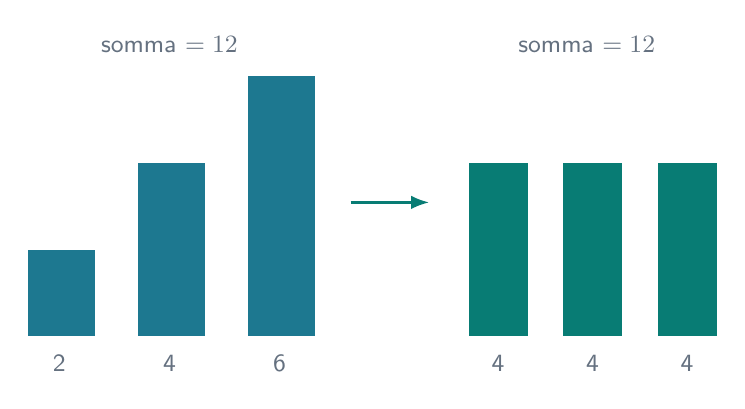
\begin{tikzpicture}[x=1cm,y=1cm]
\foreach \x/\h in {.7/1.1,2.1/2.2,3.5/3.3}{\fill[GeoA](\x,0)rectangle++(.85,\h);}
\foreach \x/\v in {1.1/2,2.5/4,3.9/6}{\node[pNote] at(\x,-.35){\v};}
\draw[pEdge](4.8,1.7)--(5.8,1.7);
\foreach \x in {6.3,7.5,8.7}{\fill[Classical](\x,0)rectangle++(.75,2.2);\node[pNote] at(\x+.375,-.35){4};}
\node[pNote] at(2.5,3.7){somma $=12$};\node[pNote] at(7.8,3.7){somma $=12$};
\end{tikzpicture}
\[\bar x=\frac{1}{n}\sum_{i=1}^{n}x_i,\qquad n\bar x=\sum_{i=1}^{n}x_i.\]
\PSmall{$n>0$ è la numerosità; $x_i$ è il valore dell'unità $i$. La media ha la stessa unità di misura di $x$.}

\end{minipage}% 
\end{lrbox}
\typeout{FULLBOX:016:L:\the\ht\PilotLeftBox:\the\dp\PilotLeftBox}
\begin{lrbox}{\PilotRightBox}%
\begin{minipage}[t]{7.55cm}\raggedright\color{Ink}\fontsize{11.3}{14.8}\selectfont

\PCode{R · somma e media}{16_media.R}
\PBody{Per i 160 fossili, la media del diametro totale è circa $6{,}355\,\mu\mathrm m$. È il valore che, ripetuto 160 volte, conserva la somma dei diametri.}

\end{minipage}% 
\end{lrbox}
\typeout{FULLBOX:016:R:\the\ht\PilotRightBox:\the\dp\PilotRightBox}
\begin{frame}[plain]\hypertarget{slide16}{}
\bookmark[level=1,page=16]{La media aritmetica conserva il totale}
\begin{tikzpicture}[remember picture,overlay]
\PilotChrome{La media aritmetica conserva il totale}{MISURE DI POSIZIONE}{16}{La media aritmetica dipende da tutti i valori e conserva il totale quando viene moltiplicata per la numerosità.}
\node[anchor=north west,inner sep=0] at ([xshift=0.96cm,yshift=-2.13cm]current page.north west) {\usebox{\PilotLeftBox}};
\node[anchor=north west,inner sep=0] at ([xshift=11.52cm,yshift=-2.13cm]current page.north west) {\usebox{\PilotRightBox}};

\end{tikzpicture}\end{frame}

% SLIDE 017 | La media minimizza gli scarti quadratici
\begin{lrbox}{\PilotLeftBox}%
\begin{minipage}[t]{10.05cm}\raggedright\color{Ink}\fontsize{11.3}{14.8}\selectfont

\PLabel{Un criterio esplicito per scegliere il centro}
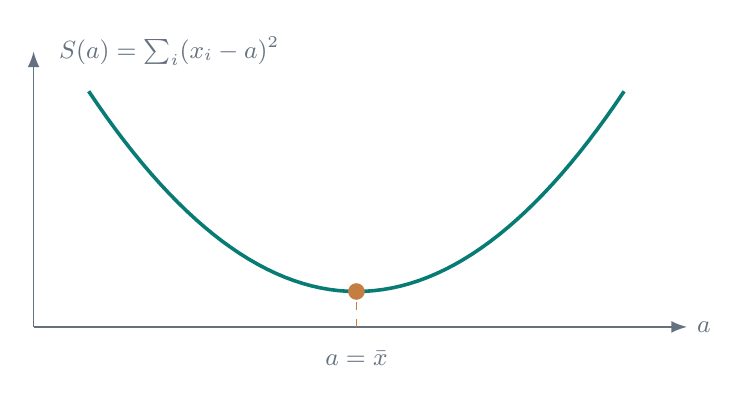
\begin{tikzpicture}[x=1cm,y=1cm]
\draw[pAxis](.8,.2)--(9.1,.2)node[right,pNote]{$a$};
\draw[pAxis](.8,.2)--(.8,3.7);
\draw[Classical,line width=1.3pt] plot[domain=1.5:8.3,samples=61](\x,{.65+.22*(\x-4.9)^2});
\draw[GeoB,dashed](4.9,.2)--(4.9,.65);\fill[GeoB](4.9,.65)circle(3pt);
\node[pNote] at(4.9,-.2){$a=\bar x$};
\node[pNote,anchor=west] at(1,3.7){$S(a)=\sum_i(x_i-a)^2$};
\end{tikzpicture}
\[S(a)=\sum_i(x_i-\bar x)^2+n(a-\bar x)^2.\]
\PBody{Il secondo termine è non negativo e si annulla solo per $a=\bar x$. La media è quindi il minimo unico, per $n>0$.}

\end{minipage}% 
\end{lrbox}
\typeout{FULLBOX:017:L:\the\ht\PilotLeftBox:\the\dp\PilotLeftBox}
\begin{lrbox}{\PilotRightBox}%
\begin{minipage}[t]{7.55cm}\raggedright\color{Ink}\fontsize{11.3}{14.8}\selectfont

\PCode{R · valutare il criterio}{17_quadrati.R}
\PSmall{Il diagramma mostra la forma del criterio. Nel caso numerico $x=(2,4,6)$, $S(4)=8$ mentre $S(3)=S(5)=11$.}
\PInfo{Elevare al quadrato aumenta l'influenza degli scarti grandi. La sensibilità ai valori estremi deriva anche da questo criterio.}

\end{minipage}% 
\end{lrbox}
\typeout{FULLBOX:017:R:\the\ht\PilotRightBox:\the\dp\PilotRightBox}
\begin{frame}[plain]\hypertarget{slide17}{}
\bookmark[level=1,page=17]{La media minimizza gli scarti quadratici}
\begin{tikzpicture}[remember picture,overlay]
\PilotChrome{La media minimizza gli scarti quadratici}{MISURE DI POSIZIONE}{17}{La media è il centro che minimizza la somma degli scarti al quadrato; il risultato dipende dal criterio adottato.}
\node[anchor=north west,inner sep=0] at ([xshift=0.96cm,yshift=-2.13cm]current page.north west) {\usebox{\PilotLeftBox}};
\node[anchor=north west,inner sep=0] at ([xshift=11.52cm,yshift=-2.13cm]current page.north west) {\usebox{\PilotRightBox}};

\end{tikzpicture}\end{frame}

% SLIDE 018 | La mediana si determina dall’ordine
\begin{lrbox}{\PilotLeftBox}%
\begin{minipage}[t]{10.05cm}\raggedright\color{Ink}\fontsize{11.3}{14.8}\selectfont

\PLabel{Posizioni centrali nel campione ordinato}
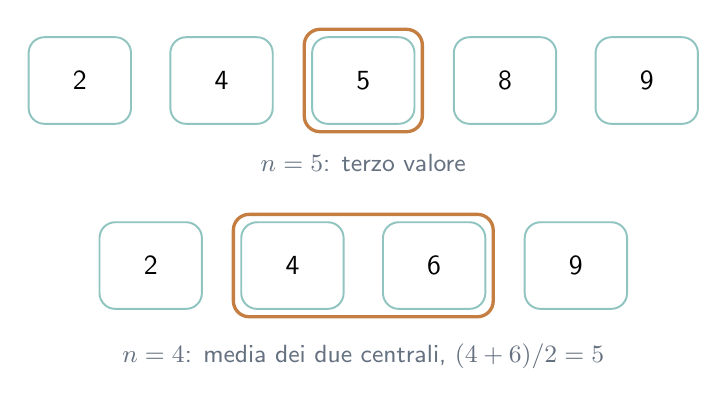
\begin{tikzpicture}[x=1cm,y=1cm]
\foreach \x/\v in {1/2,2.8/4,4.6/5,6.4/8,8.2/9}{\node[pFlow,minimum width=1.3cm] at(\x,2.7){\v};}
\draw[GeoB,line width=1.2pt,rounded corners=2mm](3.85,2.05)rectangle(5.35,3.35);
\node[pNote] at(4.6,1.65){$n=5$: terzo valore};
\foreach \x/\v in {1.9/2,3.7/4,5.5/6,7.3/9}{\node[pFlow,minimum width=1.3cm] at(\x,.35){\v};}
\draw[GeoB,line width=1.2pt,rounded corners=2mm](2.95,-.3)rectangle(6.25,1.0);
\node[pNote] at(4.6,-.8){$n=4$: media dei due centrali, $(4+6)/2=5$};
\end{tikzpicture}
\PSmall{Indicando con $x_{(i)}$ il valore in posizione $i$ dopo l'ordinamento, la mediana usa $x_{((n+1)/2)}$ se $n$ è dispari.}

\end{minipage}% 
\end{lrbox}
\typeout{FULLBOX:018:L:\the\ht\PilotLeftBox:\the\dp\PilotLeftBox}
\begin{lrbox}{\PilotRightBox}%
\begin{minipage}[t]{7.55cm}\raggedright\color{Ink}\fontsize{11.3}{14.8}\selectfont

\PCode{R · ordinare e trovare il centro}{18_mediana.R}
\PBody{Per $n$ pari, R restituisce la media dei due valori centrali:}
\[\widetilde x=\frac{x_{(n/2)}+x_{(n/2+1)}}{2}.\]
\PSmall{Almeno metà dei valori è minore o uguale alla mediana e almeno metà è maggiore o uguale. Le uguaglianze sono possibili.}

\end{minipage}% 
\end{lrbox}
\typeout{FULLBOX:018:R:\the\ht\PilotRightBox:\the\dp\PilotRightBox}
\begin{frame}[plain]\hypertarget{slide18}{}
\bookmark[level=1,page=18]{La mediana si determina dall’ordine}
\begin{tikzpicture}[remember picture,overlay]
\PilotChrome{La mediana si determina dall’ordine}{MISURE DI POSIZIONE}{18}{La mediana dipende dalle posizioni nell’ordinamento e può assumere un valore non presente nel campione.}
\node[anchor=north west,inner sep=0] at ([xshift=0.96cm,yshift=-2.13cm]current page.north west) {\usebox{\PilotLeftBox}};
\node[anchor=north west,inner sep=0] at ([xshift=11.52cm,yshift=-2.13cm]current page.north west) {\usebox{\PilotRightBox}};

\end{tikzpicture}\end{frame}

% SLIDE 019 | La mediana minimizza gli scarti assoluti
\begin{lrbox}{\PilotLeftBox}%
\begin{minipage}[t]{10.05cm}\raggedright\color{Ink}\fontsize{11.3}{14.8}\selectfont

\PLabel{Cambiare criterio cambia la misura di posizione}
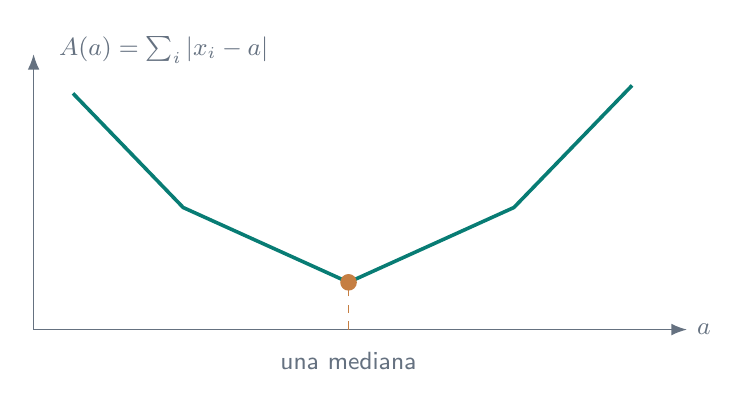
\begin{tikzpicture}[x=1cm,y=1cm]
\draw[pAxis](.8,.2)--(9.1,.2)node[right,pNote]{$a$};
\draw[pAxis](.8,.2)--(.8,3.7);
\draw[Classical,line width=1.3pt](1.3,3.2)--(2.7,1.75)--(4.8,.8)--(6.9,1.75)--(8.4,3.3);
\draw[GeoB,dashed](4.8,.2)--(4.8,.8);\fill[GeoB](4.8,.8)circle(3pt);
\node[pNote] at(4.8,-.2){una mediana};
\node[pNote,anchor=west] at(1,3.75){$A(a)=\sum_i|x_i-a|$};
\end{tikzpicture}
\PBody{Una mediana minimizza $A(a)$. Con $n$ pari, tutti i punti tra i due valori centrali minimizzano il criterio; R sceglie il loro punto medio.}
\PSmall{Lo schema illustra il criterio per un numero dispari di osservazioni. La funzione è lineare a tratti.}

\end{minipage}% 
\end{lrbox}
\typeout{FULLBOX:019:L:\the\ht\PilotLeftBox:\the\dp\PilotLeftBox}
\begin{lrbox}{\PilotRightBox}%
\begin{minipage}[t]{7.55cm}\raggedright\color{Ink}\fontsize{11.3}{14.8}\selectfont

\PCode{R · confrontare scarti assoluti}{19_assoluti.R}
\PInfo{Per il campione $(4,6)$, ogni $a\in[4,6]$ dà $|4-a|+|6-a|=2$. Il criterio, in questo caso, non ha un unico minimo.}
\PSmall{La mediana conserva l'unità della variabile, come la media. L'uso dipende dalla domanda e dalla forma dei dati.}

\end{minipage}% 
\end{lrbox}
\typeout{FULLBOX:019:R:\the\ht\PilotRightBox:\the\dp\PilotRightBox}
\begin{frame}[plain]\hypertarget{slide19}{}
\bookmark[level=1,page=19]{La mediana minimizza gli scarti assoluti}
\begin{tikzpicture}[remember picture,overlay]
\PilotChrome{La mediana minimizza gli scarti assoluti}{MISURE DI POSIZIONE}{19}{Il centro che minimizza gli scarti assoluti è una mediana; con numerosità pari il minimo può essere un intervallo.}
\node[anchor=north west,inner sep=0] at ([xshift=0.96cm,yshift=-2.13cm]current page.north west) {\usebox{\PilotLeftBox}};
\node[anchor=north west,inner sep=0] at ([xshift=11.52cm,yshift=-2.13cm]current page.north west) {\usebox{\PilotRightBox}};

\end{tikzpicture}\end{frame}

% SLIDE 020 | Quanto pesa un valore molto distante?
\begin{lrbox}{\PilotLeftBox}%
\begin{minipage}[t]{10.05cm}\raggedright\color{Ink}\fontsize{11.3}{14.8}\selectfont

\PLabel{Una perturbazione controllata}
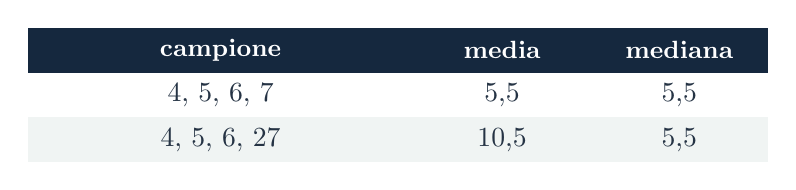
\begin{tikzpicture}[x=1cm,y=1cm]
\fill[Navy] (0,0) rectangle (9.4,0.57);
\node[font=\bfseries\fontsize{9.2}{11}\selectfont,text=white] at (2.45,0.285) {campione};
\node[font=\bfseries\fontsize{9.2}{11}\selectfont,text=white] at (6.025,0.285) {media};
\node[font=\bfseries\fontsize{9.2}{11}\selectfont,text=white] at (8.275,0.285) {mediana};
\fill[white] (0,-0.57) rectangle (9.4,0.0);
\node[font=\fontsize{9.6}{12}\selectfont,text=Ink] at (2.45,-0.285) {4, 5, 6, 7};
\node[font=\fontsize{9.6}{12}\selectfont,text=Ink] at (6.025,-0.285) {5,5};
\node[font=\fontsize{9.6}{12}\selectfont,text=Ink] at (8.275,-0.285) {5,5};
\fill[GeoTint] (0,-1.14) rectangle (9.4,-0.57);
\node[font=\fontsize{9.6}{12}\selectfont,text=Ink] at (2.45,-0.855) {4, 5, 6, 27};
\node[font=\fontsize{9.6}{12}\selectfont,text=Ink] at (6.025,-0.855) {10,5};
\node[font=\fontsize{9.6}{12}\selectfont,text=Ink] at (8.275,-0.855) {5,5};
\end{tikzpicture}
\vspace{4mm}
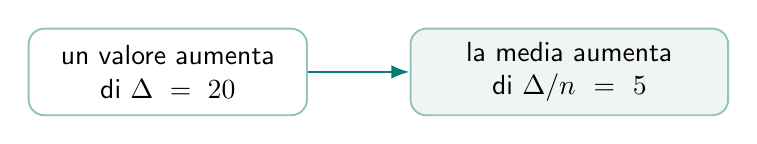
\begin{tikzpicture}[x=1cm,y=1cm]
\node[pFlow,text width=3.3cm] (a) at(2,1){un valore aumenta\\di $\Delta=20$};
\node[pFlow,text width=3.8cm,fill=GeoTint] (b) at(7.1,1){la media aumenta\\di $\Delta/n=5$};
\draw[pEdge](a)--(b);
\end{tikzpicture}
\PBody{In questo esempio la mediana resta invariata perché i valori centrali restano 5 e 6. Un cambiamento dell'ordine può modificare anche la mediana.}

\end{minipage}% 
\end{lrbox}
\typeout{FULLBOX:020:L:\the\ht\PilotLeftBox:\the\dp\PilotLeftBox}
\begin{lrbox}{\PilotRightBox}%
\begin{minipage}[t]{7.55cm}\raggedright\color{Ink}\fontsize{11.3}{14.8}\selectfont

\PCode{R · isolare l’effetto di un valore}{20_sensibilita.R}
\PInfo{Un valore distante richiede un controllo della misura e del contesto. La distanza dal centro non basta per dichiararlo errato o eliminarlo.}
\PSmall{I dati della tabella sono costruiti e adimensionali. L'identità $\Delta\bar x=\Delta/n$ vale quando cambia una sola osservazione.}

\end{minipage}% 
\end{lrbox}
\typeout{FULLBOX:020:R:\the\ht\PilotRightBox:\the\dp\PilotRightBox}
\begin{frame}[plain]\hypertarget{slide20}{}
\bookmark[level=1,page=20]{Quanto pesa un valore molto distante?}
\begin{tikzpicture}[remember picture,overlay]
\PilotChrome{Quanto pesa un valore molto distante?}{MISURE DI POSIZIONE}{20}{La sensibilità di una statistica va valutata rispetto al tipo di perturbazione che si sta introducendo.}
\node[anchor=north west,inner sep=0] at ([xshift=0.96cm,yshift=-2.13cm]current page.north west) {\usebox{\PilotLeftBox}};
\node[anchor=north west,inner sep=0] at ([xshift=11.52cm,yshift=-2.13cm]current page.north west) {\usebox{\PilotRightBox}};

\end{tikzpicture}\end{frame}

% SLIDE 021 | La media fisicamente pertinente: densità
\begin{lrbox}{\PilotLeftBox}%
\begin{minipage}[t]{10.05cm}\raggedright\color{Ink}\fontsize{11.3}{14.8}\selectfont

\PLabel{Il rapporto tra totali determina i pesi}
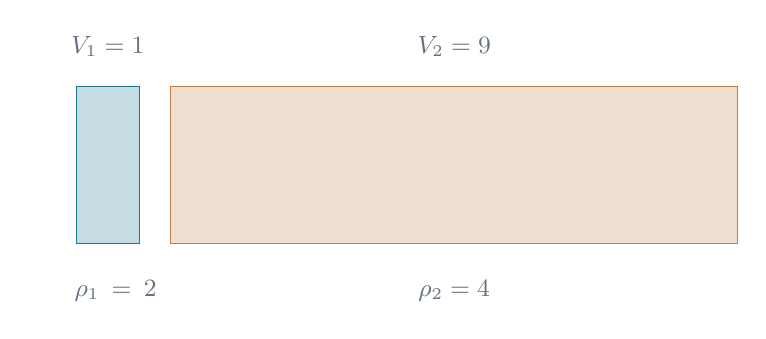
\begin{tikzpicture}[x=1cm,y=1cm]
\fill[GeoA!25,draw=GeoA](.5,.3)rectangle(1.3,2.3);
\fill[GeoB!25,draw=GeoB](1.7,.3)rectangle(8.9,2.3);
\node[pNote] at(.9,2.8){$V_1=1$};\node[pNote] at(5.3,2.8){$V_2=9$};
\node[pNote,text width=2cm] at(1,-.3){$\rho_1=2$};\node[pNote] at(5.3,-.3){$\rho_2=4$};
\end{tikzpicture}
\[\rho_{\mathrm{tot}}=\frac{\sum_i m_i}{\sum_i V_i}
 =\frac{\sum_i V_i\rho_i}{\sum_i V_i}=3{,}8\,\mathrm{g/cm^3}.\]
\PSmall{Volumi in cm$^3$, densità in g/cm$^3$. Il disegno assegna ai due provini aree proporzionali al volume: esempio numerico costruito.}
\PSmall{La media delle densità individuali vale 3. Il rapporto fra massa totale e volume totale usa i volumi come pesi.}

\end{minipage}% 
\end{lrbox}
\typeout{FULLBOX:021:L:\the\ht\PilotLeftBox:\the\dp\PilotLeftBox}
\begin{lrbox}{\PilotRightBox}%
\begin{minipage}[t]{7.55cm}\raggedright\color{Ink}\fontsize{11.3}{14.8}\selectfont

\PCode{R · individuare il peso corretto}{21_densita.R}
\PInfo{La formula riguarda la somma dei volumi misurati. Per un miscuglio reale occorre verificare se volume, porosità o compattazione cambiano durante l'unione.}

\end{minipage}% 
\end{lrbox}
\typeout{FULLBOX:021:R:\the\ht\PilotRightBox:\the\dp\PilotRightBox}
\begin{frame}[plain]\hypertarget{slide21}{}
\bookmark[level=1,page=21]{La media fisicamente pertinente: densità}
\begin{tikzpicture}[remember picture,overlay]
\PilotChrome{La media fisicamente pertinente: densità}{MISURE DI POSIZIONE}{21}{Il peso corretto deriva dalla quantità fisica che si vuole calcolare e dalle ipotesi sui totali.}
\node[anchor=north west,inner sep=0] at ([xshift=0.96cm,yshift=-2.13cm]current page.north west) {\usebox{\PilotLeftBox}};
\node[anchor=north west,inner sep=0] at ([xshift=11.52cm,yshift=-2.13cm]current page.north west) {\usebox{\PilotRightBox}};

\end{tikzpicture}\end{frame}

% SLIDE 022 | Moda, ripetizioni e risoluzione delle misure
\begin{lrbox}{\PilotLeftBox}%
\begin{minipage}[t]{10.05cm}\raggedright\color{Ink}\fontsize{11.3}{14.8}\selectfont

\PLabel{La categoria o il valore più frequente}
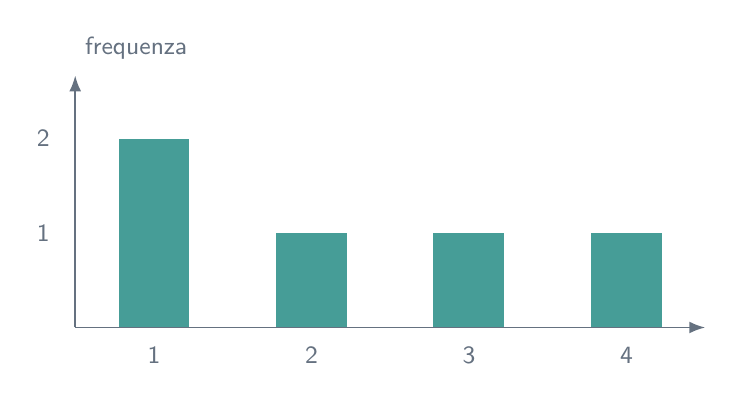
\begin{tikzpicture}[x=1cm,y=1cm]
\draw[pAxis](1,0)--(9,0);\draw[pAxis](1,0)--(1,3.2);
\foreach \x/\h/\v in {2/2.4/1,4/1.2/2,6/1.2/3,8/1.2/4}{
\fill[Classical!75](\x-.45,0)rectangle(\x+.45,\h);\node[pNote] at(\x,-.35){\v};}
\node[pNote,anchor=east] at(.8,1.2){1};\node[pNote,anchor=east] at(.8,2.4){2};
\node[pNote,anchor=west] at(1,3.55){frequenza};
\end{tikzpicture}
\PBody{La moda può essere multipla. Nei fossili, i due morfotipi hanno frequenza 80: entrambe le categorie sono modali.}
\PSmall{Per misure continue, arrotondamento e scelta delle classi influenzano le ripetizioni. La classe più frequente dipende dai suoi confini.}

\end{minipage}% 
\end{lrbox}
\typeout{FULLBOX:022:L:\the\ht\PilotLeftBox:\the\dp\PilotLeftBox}
\begin{lrbox}{\PilotRightBox}%
\begin{minipage}[t]{7.55cm}\raggedright\color{Ink}\fontsize{11.3}{14.8}\selectfont

\PCode{R · ricavare tutte le mode}{22_moda.R}
\PBody{La selezione conserva tutti i valori con frequenza massima. Il nome della funzione \texttt{mode()} in R ha un significato informatico diverso.}

\end{minipage}% 
\end{lrbox}
\typeout{FULLBOX:022:R:\the\ht\PilotRightBox:\the\dp\PilotRightBox}
\begin{frame}[plain]\hypertarget{slide22}{}
\bookmark[level=1,page=22]{Moda, ripetizioni e risoluzione delle misure}
\begin{tikzpicture}[remember picture,overlay]
\PilotChrome{Moda, ripetizioni e risoluzione delle misure}{MISURE DI POSIZIONE}{22}{La moda descrive la frequenza massima; la sua interpretazione richiede di conoscere categorie, risoluzione e raggruppamenti.}
\node[anchor=north west,inner sep=0] at ([xshift=0.96cm,yshift=-2.13cm]current page.north west) {\usebox{\PilotLeftBox}};
\node[anchor=north west,inner sep=0] at ([xshift=11.52cm,yshift=-2.13cm]current page.north west) {\usebox{\PilotRightBox}};

\end{tikzpicture}\end{frame}

% SLIDE 023 | Laboratorio: media e mediana sotto perturbazione
\begin{lrbox}{\PilotLeftBox}%
\begin{minipage}[t]{10.05cm}\raggedright\color{Ink}\fontsize{11.3}{14.8}\selectfont

\PLabel{Esperimento m03-posizione}
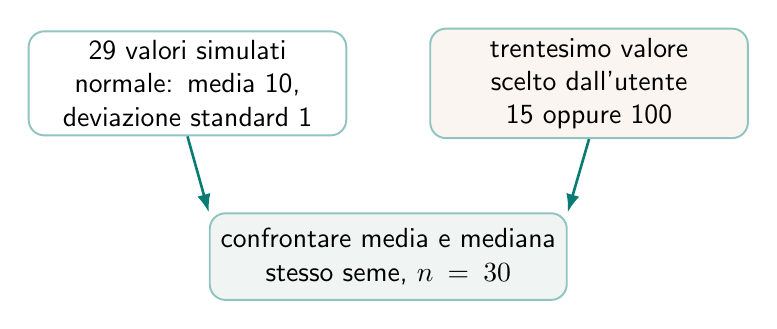
\begin{tikzpicture}[x=1cm,y=1cm]
\node[pFlow,text width=3.8cm] (a) at(2.1,2.7){29 valori simulati\\normale: media 10,\\deviazione standard 1};
\node[pFlow,text width=3.8cm,fill=GeoB!8] (b) at(7.2,2.7){trentesimo valore\\scelto dall'utente\\15 oppure 100};
\node[pFlow,text width=4.3cm,fill=GeoTint] (c) at(4.65,.5){confrontare media e mediana\\stesso seme, $n=30$};
\draw[pEdge](a.south)--(c.north west);\draw[pEdge](b.south)--(c.north east);
\end{tikzpicture}
\PBody{Prevedere la variazione della media: $(100-15)/30\simeq2{,}833$. Verificare il risultato e spiegare il comportamento della mediana osservata.}
\PSmall{\href{https://marzione00.github.io/Lab_Geo/\#laboratorio/m03-posizione}{Apri l'esperimento · Media e mediana sotto contaminazione}}

\end{minipage}% 
\end{lrbox}
\typeout{FULLBOX:023:L:\the\ht\PilotLeftBox:\the\dp\PilotLeftBox}
\begin{lrbox}{\PilotRightBox}%
\begin{minipage}[t]{7.55cm}\raggedright\color{Ink}\fontsize{11.3}{14.8}\selectfont

\PCode{R · una previsione da verificare}{23_lab_posizione.R}
\PInfo{Con il seme fissato, i primi 29 valori coincidono nei due scenari. Il confronto isola l'effetto del trentesimo valore.}
\PSmall{Nel quaderno distinguere la variazione prevista dalla formula e i valori della media e della mediana calcolati sul campione simulato.}

\end{minipage}% 
\end{lrbox}
\typeout{FULLBOX:023:R:\the\ht\PilotRightBox:\the\dp\PilotRightBox}
\begin{frame}[plain]\hypertarget{slide23}{}
\bookmark[level=1,page=23]{Laboratorio: media e mediana sotto perturbazione}
\begin{tikzpicture}[remember picture,overlay]
\PilotChrome{Laboratorio: media e mediana sotto perturbazione}{LABORATORIO · POSIZIONE}{23}{Un confronto controllato modifica un elemento e conserva gli altri ingressi: la differenza osservata diventa interpretabile.}
\node[anchor=north west,inner sep=0] at ([xshift=0.96cm,yshift=-2.13cm]current page.north west) {\usebox{\PilotLeftBox}};
\node[anchor=north west,inner sep=0] at ([xshift=11.52cm,yshift=-2.13cm]current page.north west) {\usebox{\PilotRightBox}};

\end{tikzpicture}\end{frame}

% SLIDE 024 | Stessa media, dispersione diversa
\begin{lrbox}{\PilotLeftBox}%
\begin{minipage}[t]{10.05cm}\raggedright\color{Ink}\fontsize{11.3}{14.8}\selectfont

\PLabel{Due serie costruite, espresse in millimetri}
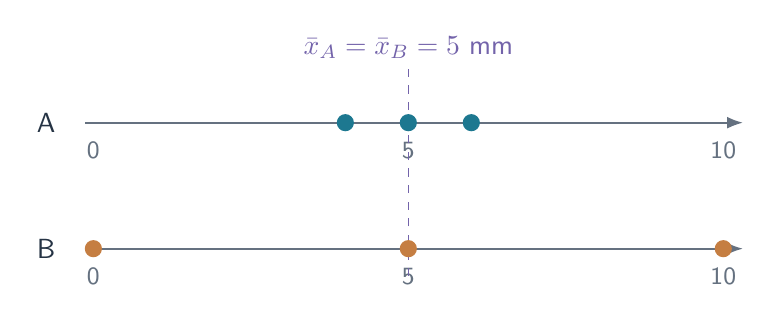
\begin{tikzpicture}[x=1cm,y=1cm]
 \foreach \y/\lab in {2.3/A,0.7/B}{
  \node[pLabel] at (.25,\y) {\lab};
  \draw[pAxis] (.75,\y)--(9.1,\y);
  \foreach \v in {0,5,10}{\node[pNote,below] at ({.85+.8*\v},\y-.12) {\v};}
 }
 \draw[GeoC,dashed] (4.85,.35)--(4.85,3);
 \foreach \v in {4,5,6}{\fill[GeoA] ({.85+.8*\v},2.3) circle(3.1pt);}
 \foreach \v in {0,5,10}{\fill[GeoB] ({.85+.8*\v},.7) circle(3.1pt);}
 \node[pLabel,text=GeoC] at (4.85,3.25) {$\bar x_A=\bar x_B=5$ mm};
\end{tikzpicture}
\PBody{La media individua lo stesso centro. Le distanze dal centro sono maggiori nella serie B.}
\[s_A=1\;\mathrm{mm},\qquad s_B=5\;\mathrm{mm}.\]

\end{minipage}% 
\end{lrbox}
\typeout{FULLBOX:024:L:\the\ht\PilotLeftBox:\the\dp\PilotLeftBox}
\begin{lrbox}{\PilotRightBox}%
\begin{minipage}[t]{7.55cm}\raggedright\color{Ink}\fontsize{11.3}{14.8}\selectfont

\PCode{R · aggiungere una misura di dispersione}{24_dispersione.R}
\PSmall{\texttt{c()} costruisce ciascuna serie; \texttt{rbind()} affianca i risultati per righe. \texttt{sd()} calcola la deviazione standard.}
\PInfo{Una sintesi utile riferisce insieme posizione, dispersione e numero di osservazioni.}

\end{minipage}% 
\end{lrbox}
\typeout{FULLBOX:024:R:\the\ht\PilotRightBox:\the\dp\PilotRightBox}
\begin{frame}[plain]\hypertarget{slide24}{}
\bookmark[level=1,page=24]{Stessa media, dispersione diversa}
\begin{tikzpicture}[remember picture,overlay]
\PilotChrome{Stessa media, dispersione diversa}{DISPERSIONE E QUANTILI}{24}{Due serie con la stessa media possono avere distanze dal centro molto diverse.}
\node[anchor=north west,inner sep=0] at ([xshift=0.96cm,yshift=-2.13cm]current page.north west) {\usebox{\PilotLeftBox}};
\node[anchor=north west,inner sep=0] at ([xshift=11.52cm,yshift=-2.13cm]current page.north west) {\usebox{\PilotRightBox}};

\end{tikzpicture}\end{frame}

% SLIDE 025 | Gli scarti con segno si compensano
\begin{lrbox}{\PilotLeftBox}%
\begin{minipage}[t]{10.05cm}\raggedright\color{Ink}\fontsize{11.3}{14.8}\selectfont

\PLabel{Dalla posizione alla distanza}
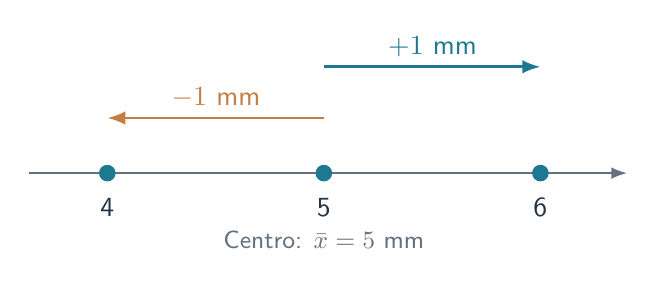
\begin{tikzpicture}[x=1cm,y=1cm]
 \draw[pAxis] (1,1.4)--(8.6,1.4);
 \foreach \x/\v in {2/4,4.75/5,7.5/6}{\fill[GeoA] (\x,1.4) circle(3pt);\node[pLabel,below] at (\x,1.2) {\v};}
 \draw[pEdge,GeoB] (4.75,2.1)--(2,2.1);
 \draw[pEdge,GeoA] (4.75,2.75)--(7.5,2.75);
 \node[pLabel,above,text=GeoB] at (3.38,2.1) {$-1$ mm};
 \node[pLabel,above,text=GeoA] at (6.13,2.75) {$+1$ mm};
 \node[pNote] at (4.75,.55) {Centro: $\bar x=5$ mm};
\end{tikzpicture}
\[d_i=x_i-\bar x,\qquad \sum_{i=1}^{n}d_i=0.\]
\PSmall{$d_i$ è lo scarto della misura $i$ dal centro. Gli scarti con segno non misurano la dispersione perché si annullano nella somma.}

\end{minipage}% 
\end{lrbox}
\typeout{FULLBOX:025:L:\the\ht\PilotLeftBox:\the\dp\PilotLeftBox}
\begin{lrbox}{\PilotRightBox}%
\begin{minipage}[t]{7.55cm}\raggedright\color{Ink}\fontsize{11.3}{14.8}\selectfont

\PLabel{Elevare al quadrato}
\[(-1)^2+0^2+1^2=2\;\mathrm{mm}^2.\]
\PBody{Il quadrato rende positivi i contributi dei due lati del centro e attribuisce più peso alle distanze grandi.}
\PInfo{Raddoppiare uno scarto moltiplica per quattro il suo contributo alla somma dei quadrati.}
\PSmall{La distanza assoluta è un'altra scelta; conduce a indicatori con proprietà diverse.}

\end{minipage}% 
\end{lrbox}
\typeout{FULLBOX:025:R:\the\ht\PilotRightBox:\the\dp\PilotRightBox}
\begin{frame}[plain]\hypertarget{slide25}{}
\bookmark[level=1,page=25]{Gli scarti con segno si compensano}
\begin{tikzpicture}[remember picture,overlay]
\PilotChrome{Gli scarti con segno si compensano}{DISPERSIONE E QUANTILI}{25}{La somma degli scarti dalla media è nulla. Per descrivere la dispersione occorre trasformare le distanze.}
\node[anchor=north west,inner sep=0] at ([xshift=0.96cm,yshift=-2.13cm]current page.north west) {\usebox{\PilotLeftBox}};
\node[anchor=north west,inner sep=0] at ([xshift=11.52cm,yshift=-2.13cm]current page.north west) {\usebox{\PilotRightBox}};

\end{tikzpicture}\end{frame}

% SLIDE 026 | Varianza e deviazione standard
\begin{lrbox}{\PilotLeftBox}%
\begin{minipage}[t]{10.05cm}\raggedright\color{Ink}\fontsize{11.3}{14.8}\selectfont

\PLabel{La convenzione di var() e sd()}
\[s^2=\frac{1}{n-1}\sum_{i=1}^{n}(x_i-\bar x)^2,
\qquad s=\sqrt{s^2}.\]
\PSmall{$n>1$: numero di misure finite; $s^2$: varianza; $s$: deviazione standard. Con misure in mm, le unità sono mm$^2$ e mm.}
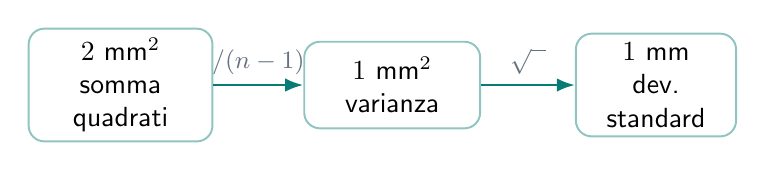
\begin{tikzpicture}[x=1cm,y=1cm]
 \node[pFlow,text width=2.1cm] (a) at (1.25,1) {$2$ mm$^2$\\somma quadrati};
 \node[pFlow,text width=2cm] (b) at (4.7,1) {$1$ mm$^2$\\varianza};
 \node[pFlow,text width=1.8cm] (c) at (8.05,1) {$1$ mm\\dev. standard};
 \draw[pEdge] (a)--node[pNote,above] {$/(n-1)$} (b);
 \draw[pEdge] (b)--node[pNote,above] {$\sqrt{\phantom{x}}$} (c);
\end{tikzpicture}
\PSmall{Qui descriviamo i dati. L'interpretazione di $s^2$ come stima non distorta richiede un campione indipendente, stessa distribuzione e varianza finita.}

\end{minipage}% 
\end{lrbox}
\typeout{FULLBOX:026:L:\the\ht\PilotLeftBox:\the\dp\PilotLeftBox}
\begin{lrbox}{\PilotRightBox}%
\begin{minipage}[t]{7.55cm}\raggedright\color{Ink}\fontsize{11.3}{14.8}\selectfont

\PCode{R · ricostruire il calcolo}{26_varianza.R}
\PSmall{\texttt{length()} conta i valori. Il confronto verifica che la formula coincide con \texttt{var()}.}
\PInfo{La divisione per $n-1$ è la convenzione usata qui. La media dei quadrati con denominatore $n$ è una quantità diversa.}

\end{minipage}% 
\end{lrbox}
\typeout{FULLBOX:026:R:\the\ht\PilotRightBox:\the\dp\PilotRightBox}
\begin{frame}[plain]\hypertarget{slide26}{}
\bookmark[level=1,page=26]{Varianza e deviazione standard}
\begin{tikzpicture}[remember picture,overlay]
\PilotChrome{Varianza e deviazione standard}{DISPERSIONE E QUANTILI}{26}{La varianza ha unità al quadrato; la deviazione standard torna all’unità della misura.}
\node[anchor=north west,inner sep=0] at ([xshift=0.96cm,yshift=-2.13cm]current page.north west) {\usebox{\PilotLeftBox}};
\node[anchor=north west,inner sep=0] at ([xshift=11.52cm,yshift=-2.13cm]current page.north west) {\usebox{\PilotRightBox}};

\end{tikzpicture}\end{frame}

% SLIDE 027 | Cambiare unità cambia anche la dispersione
\begin{lrbox}{\PilotLeftBox}%
\begin{minipage}[t]{10.05cm}\raggedright\color{Ink}\fontsize{11.3}{14.8}\selectfont

\PLabel{Da millimetri a micrometri}
\begin{tikzpicture}[x=1cm,y=1cm]
 \node[pFlow,text width=3.2cm] (a) at (2,1.7) {$4,\;5,\;6$ mm\\$s=1$ mm};
 \node[pFlow,text width=3.6cm] (b) at (7.25,1.7) {$4000,\;5000,\;6000$ $\mu$m\\$s=1000$ $\mu$m};
 \draw[pEdge] (a)--node[pNote,above] {$\times1000$} (b);
\end{tikzpicture}
\[y_i=a+bx_i:\qquad s_y=|b|s_x,\quad s_y^2=b^2s_x^2.\]
\PSmall{La costante $a$ sposta tutte le misure della stessa quantità e lascia uguali le distanze. Il fattore $b$ ne cambia la scala.}
\PInfo{$1\;\mathrm{mm}^2=10^6\;\mu\mathrm{m}^2$: convertire una varianza richiede il quadrato del fattore di conversione.}

\end{minipage}% 
\end{lrbox}
\typeout{FULLBOX:027:L:\the\ht\PilotLeftBox:\the\dp\PilotLeftBox}
\begin{lrbox}{\PilotRightBox}%
\begin{minipage}[t]{7.55cm}\raggedright\color{Ink}\fontsize{11.3}{14.8}\selectfont

\PCode{R · conversione e traslazione}{27_unita.R}
\PSmall{La prima operazione cambia l'unità. L'ultima aggiunge 20 mm a ogni misura: la deviazione standard rimane 1 mm.}

\end{minipage}% 
\end{lrbox}
\typeout{FULLBOX:027:R:\the\ht\PilotRightBox:\the\dp\PilotRightBox}
\begin{frame}[plain]\hypertarget{slide27}{}
\bookmark[level=1,page=27]{Cambiare unità cambia anche la dispersione}
\begin{tikzpicture}[remember picture,overlay]
\PilotChrome{Cambiare unità cambia anche la dispersione}{DISPERSIONE E QUANTILI}{27}{Prima di confrontare deviazioni standard, verificare che variabile, unità e convenzione di calcolo coincidano.}
\node[anchor=north west,inner sep=0] at ([xshift=0.96cm,yshift=-2.13cm]current page.north west) {\usebox{\PilotLeftBox}};
\node[anchor=north west,inner sep=0] at ([xshift=11.52cm,yshift=-2.13cm]current page.north west) {\usebox{\PilotRightBox}};

\end{tikzpicture}\end{frame}

% SLIDE 028 | I quantili richiedono una convenzione
\begin{lrbox}{\PilotLeftBox}%
\begin{minipage}[t]{10.05cm}\raggedright\color{Ink}\fontsize{11.3}{14.8}\selectfont

\PLabel{Ordinare i dati e interpolare: tipo 7}
\begin{tikzpicture}[x=1cm,y=1cm]
\fill[GeoTint] (0,0) rectangle (9.3,.62);
\node[font=\sffamily\fontsize{9.8}{12.1}\selectfont,anchor=west,text=Ink] at (0.120,0.310) {Posizione};
\node[font=\sffamily\fontsize{9.8}{12.1}\selectfont,anchor=west,text=Ink] at (2.220,0.310) {1};
\node[font=\sffamily\fontsize{9.8}{12.1}\selectfont,anchor=west,text=Ink] at (3.120,0.310) {2};
\node[font=\sffamily\fontsize{9.8}{12.1}\selectfont,anchor=west,text=Ink] at (4.020,0.310) {3};
\node[font=\sffamily\fontsize{9.8}{12.1}\selectfont,anchor=west,text=Ink] at (4.920,0.310) {4};
\node[font=\sffamily\fontsize{9.8}{12.1}\selectfont,anchor=west,text=Ink] at (5.820,0.310) {5};
\node[font=\sffamily\fontsize{9.8}{12.1}\selectfont,anchor=west,text=Ink] at (6.720,0.310) {6};
\node[font=\sffamily\fontsize{9.8}{12.1}\selectfont,anchor=west,text=Ink] at (7.620,0.310) {7};
\node[font=\sffamily\fontsize{9.8}{12.1}\selectfont,anchor=west,text=Ink] at (8.520,0.310) {8};
\draw[Rule] (0,0.000)--(9.3,0.000);
\node[font=\sffamily\fontsize{9.8}{12.1}\selectfont,anchor=west,text=Ink] at (0.120,-0.310) {Valore};
\node[font=\sffamily\fontsize{9.8}{12.1}\selectfont,anchor=west,text=Ink] at (2.220,-0.310) {1};
\node[font=\sffamily\fontsize{9.8}{12.1}\selectfont,anchor=west,text=Ink] at (3.120,-0.310) {2};
\node[font=\sffamily\fontsize{9.8}{12.1}\selectfont,anchor=west,text=Ink] at (4.020,-0.310) {4};
\node[font=\sffamily\fontsize{9.8}{12.1}\selectfont,anchor=west,text=Ink] at (4.920,-0.310) {7};
\node[font=\sffamily\fontsize{9.8}{12.1}\selectfont,anchor=west,text=Ink] at (5.820,-0.310) {8};
\node[font=\sffamily\fontsize{9.8}{12.1}\selectfont,anchor=west,text=Ink] at (6.720,-0.310) {9};
\node[font=\sffamily\fontsize{9.8}{12.1}\selectfont,anchor=west,text=Ink] at (7.620,-0.310) {10};
\node[font=\sffamily\fontsize{9.8}{12.1}\selectfont,anchor=west,text=Ink] at (8.520,-0.310) {12};
\draw[Rule] (0,-0.620)--(9.3,-0.620);
\end{tikzpicture}
\[h=1+(n-1)p,\quad j=\lfloor h\rfloor,\quad \gamma=h-j.\]
\[Q_7(p)=(1-\gamma)x_{(j)}+\gamma x_{(j+1)}.\]
\PSmall{$x_{(j)}$: valore in posizione $j$; $p$: quota fra 0 e 1. Per $0<p<1$ e $n>1$, si interpolano i due valori adiacenti.}
\PBody{Con $p=0{,}25$: $h=2{,}75$ e $Q_7=0{,}25\cdot2+0{,}75\cdot4=3{,}5$.}

\end{minipage}% 
\end{lrbox}
\typeout{FULLBOX:028:L:\the\ht\PilotLeftBox:\the\dp\PilotLeftBox}
\begin{lrbox}{\PilotRightBox}%
\begin{minipage}[t]{7.55cm}\raggedright\color{Ink}\fontsize{11.3}{14.8}\selectfont

\PCode{R · dichiarare il tipo di quantile}{28_quantili.R}
\PSmall{R offre nove definizioni. \texttt{type = 7} è quella predefinita e viene esplicitata per documentare il calcolo.}
\PInfo{Ai bordi: $Q(0)=\min(x)$ e $Q(1)=\max(x)$. Con un solo dato, tutti i quantili coincidono con quel valore.}

\end{minipage}% 
\end{lrbox}
\typeout{FULLBOX:028:R:\the\ht\PilotRightBox:\the\dp\PilotRightBox}
\begin{frame}[plain]\hypertarget{slide28}{}
\bookmark[level=1,page=28]{I quantili richiedono una convenzione}
\begin{tikzpicture}[remember picture,overlay]
\PilotChrome{I quantili richiedono una convenzione}{DISPERSIONE E QUANTILI}{28}{Il quantile campionario dipende dall’ordinamento e dalla regola di interpolazione; indicare la convenzione usata.}
\node[anchor=north west,inner sep=0] at ([xshift=0.96cm,yshift=-2.13cm]current page.north west) {\usebox{\PilotLeftBox}};
\node[anchor=north west,inner sep=0] at ([xshift=11.52cm,yshift=-2.13cm]current page.north west) {\usebox{\PilotRightBox}};

\end{tikzpicture}\end{frame}

% SLIDE 029 | L’intervallo interquartile
\begin{lrbox}{\PilotLeftBox}%
\begin{minipage}[t]{10.05cm}\raggedright\color{Ink}\fontsize{11.3}{14.8}\selectfont

\PLabel{Ampiezza della parte centrale}
\begin{tikzpicture}[x=1cm,y=1cm]
 \draw[pAxis] (.65,.8)--(9.2,.8);
 \foreach \v in {1,2,4,7,8,9,10,12}{\fill[Muted] ({.7+.68*\v},.8) circle(2.4pt);}
 \fill[GeoA!16] (3.08,1.35) rectangle (6.99,2.3);
 \draw[GeoA,line width=1pt] (3.08,1.35) rectangle (6.99,2.3);
 \draw[GeoC,line width=1.2pt] (5.8,1.35)--(5.8,2.3);
 \node[pNote,above] at (3.08,2.4) {$Q_{0,25}=3{,}5$};
 \node[pNote,above] at (6.99,2.4) {$Q_{0,75}=9{,}25$};
 \draw[<->,>=Latex,GeoA] (3.08,.3)--(6.99,.3);
 \node[pNote,below] at (5.04,.3) {IQR $=5{,}75$ mm};
\end{tikzpicture}
\[\operatorname{IQR}=Q_{0,75}-Q_{0,25}.\]
\PSmall{L'IQR misura una distanza nella stessa unità dei dati. Risente meno dei valori estremi rispetto alla deviazione standard.}

\end{minipage}% 
\end{lrbox}
\typeout{FULLBOX:029:L:\the\ht\PilotLeftBox:\the\dp\PilotLeftBox}
\begin{lrbox}{\PilotRightBox}%
\begin{minipage}[t]{7.55cm}\raggedright\color{Ink}\fontsize{11.3}{14.8}\selectfont

\PCode{R · sottrarre i due quartili}{29_iqr.R}
\PSmall{\texttt{diff()} sottrae il primo valore dal secondo. \texttt{IQR()} applica la stessa definizione.}
\PInfo{Con molti valori ripetuti l'IQR può essere zero anche se qualche osservazione è diversa. Conservare anche il numero di dati e la figura.}

\end{minipage}% 
\end{lrbox}
\typeout{FULLBOX:029:R:\the\ht\PilotRightBox:\the\dp\PilotRightBox}
\begin{frame}[plain]\hypertarget{slide29}{}
\bookmark[level=1,page=29]{L’intervallo interquartile}
\begin{tikzpicture}[remember picture,overlay]
\PilotChrome{L’intervallo interquartile}{DISPERSIONE E QUANTILI}{29}{L’IQR descrive l’ampiezza centrale. Può ignorare differenze presenti nelle code della distribuzione.}
\node[anchor=north west,inner sep=0] at ([xshift=0.96cm,yshift=-2.13cm]current page.north west) {\usebox{\PilotLeftBox}};
\node[anchor=north west,inner sep=0] at ([xshift=11.52cm,yshift=-2.13cm]current page.north west) {\usebox{\PilotRightBox}};

\end{tikzpicture}\end{frame}

% SLIDE 030 | Calcolare sugli stessi dati validi
\begin{lrbox}{\PilotLeftBox}%
\begin{minipage}[t]{10.05cm}\raggedright\color{Ink}\fontsize{11.3}{14.8}\selectfont

\PLabel{Il diametro dei 160 fossili simulati}
\begin{tikzpicture}[x=1cm,y=1cm]
 \node[pFlow,text width=2.2cm] (a) at (1.35,1.3) {Una colonna\\diametro totale};
 \node[pFlow,text width=2.35cm] (b) at (4.7,1.3) {Valori finiti\\e positivi};
 \node[pFlow,text width=2.2cm] (c) at (8.05,1.3) {Sintesi comune\\$n=160$};
 \draw[pEdge] (a)--(b);\draw[pEdge] (b)--(c);
\end{tikzpicture}
\PBody{Media, mediana, deviazione standard e quartili devono riferirsi alla stessa selezione di osservazioni.}
\PSmall{Controllare valori mancanti, unità e numero effettivo di misure. Nel CSV didattico i 160 diametri sono finiti e positivi.}
\PInfo{Un valore mancante richiede una scelta documentata; \texttt{na.rm = TRUE} cambia il campione su cui si calcola la sintesi.}

\end{minipage}% 
\end{lrbox}
\typeout{FULLBOX:030:L:\the\ht\PilotLeftBox:\the\dp\PilotLeftBox}
\begin{lrbox}{\PilotRightBox}%
\begin{minipage}[t]{7.55cm}\raggedright\color{Ink}\fontsize{11.3}{14.8}\selectfont

\PCode{R · verificare prima di riassumere}{30_fossili.R}
\PSmall{\texttt{stopifnot()} interrompe l'esecuzione se un controllo fallisce. Le quantità di posizione e dispersione sono in $\mu$m.}
\PSmall{Il rapporto $s/\bar x$ è interpretabile solo con uno zero fisico significativo e una media sufficientemente lontana da zero.}

\end{minipage}% 
\end{lrbox}
\typeout{FULLBOX:030:R:\the\ht\PilotRightBox:\the\dp\PilotRightBox}
\begin{frame}[plain]\hypertarget{slide30}{}
\bookmark[level=1,page=30]{Calcolare sugli stessi dati validi}
\begin{tikzpicture}[remember picture,overlay]
\PilotChrome{Calcolare sugli stessi dati validi}{DISPERSIONE E QUANTILI}{30}{Ogni indicatore deve dichiarare variabile, unità, dati ammessi e numero effettivo di osservazioni.}
\node[anchor=north west,inner sep=0] at ([xshift=0.96cm,yshift=-2.13cm]current page.north west) {\usebox{\PilotLeftBox}};
\node[anchor=north west,inner sep=0] at ([xshift=11.52cm,yshift=-2.13cm]current page.north west) {\usebox{\PilotRightBox}};

\end{tikzpicture}\end{frame}

% SLIDE 031 | Laboratorio · quantili e dispersione
\begin{lrbox}{\PilotLeftBox}%
\begin{minipage}[t]{10.05cm}\raggedright\color{Ink}\fontsize{11.3}{14.8}\selectfont

\PLabel{Iride: esperimento m03-quantili}
\begin{tikzpicture}[x=1cm,y=1cm]
 \node[pFlow,text width=3.7cm] (a) at (2.3,1.55) {$n=60$, rumore $=1$\\seme $=17$};
 \node[pFlow,text width=3.7cm] (b) at (7.2,1.55) {$n=60$, rumore $=2$\\seme $=17$};
 \draw[pEdge] (a)--(b);
 \node[pNote] at (4.75,.35) {Stessi numeri casuali, dispersione riscalata};
\end{tikzpicture}
\[X_i=10+\sigma Z_i,\qquad Z_i\sim N(0,1).\]
\PSmall{$\sigma$ è il parametro di rumore. Raddoppiarlo, a seme e numerosità fissi, raddoppia sd e IQR. Poi cambiare $n$ e osservare la variabilità dei quartili.}
\PSmall{Aprire \href{https://marzione00.github.io/Lab_Geo/}{Lab\_Geo}, pianeta Iride, esperimento \texttt{m03-quantili}.}

\end{minipage}% 
\end{lrbox}
\typeout{FULLBOX:031:L:\the\ht\PilotLeftBox:\the\dp\PilotLeftBox}
\begin{lrbox}{\PilotRightBox}%
\begin{minipage}[t]{7.55cm}\raggedright\color{Ink}\fontsize{11.3}{14.8}\selectfont

\PCode{R · riprodurre due scenari}{31_lab_quantili.R}
\PSmall{La funzione del progetto restituisce dati e indicatori. \texttt{rbind()} permette di confrontare i due risultati.}
\PInfo{Prima del calcolo, prevedere il cambiamento. Dopo il calcolo, distinguere l'effetto del parametro dalle differenze dovute a un nuovo campione.}

\end{minipage}% 
\end{lrbox}
\typeout{FULLBOX:031:R:\the\ht\PilotRightBox:\the\dp\PilotRightBox}
\begin{frame}[plain]\hypertarget{slide31}{}
\bookmark[level=1,page=31]{Laboratorio · quantili e dispersione}
\begin{tikzpicture}[remember picture,overlay]
\PilotChrome{Laboratorio · quantili e dispersione}{DISPERSIONE E QUANTILI}{31}{Variare un parametro alla volta e fissare il seme permette di attribuire il cambiamento allo scenario scelto.}
\node[anchor=north west,inner sep=0] at ([xshift=0.96cm,yshift=-2.13cm]current page.north west) {\usebox{\PilotLeftBox}};
\node[anchor=north west,inner sep=0] at ([xshift=11.52cm,yshift=-2.13cm]current page.north west) {\usebox{\PilotRightBox}};

\end{tikzpicture}\end{frame}

% SLIDE 032 | Dalle osservazioni alle classi
\begin{lrbox}{\PilotLeftBox}%
\begin{minipage}[t]{10.05cm}\raggedright\color{Ink}\fontsize{11.3}{14.8}\selectfont

\PLabel{Dieci misure in tre intervalli}
\begin{tikzpicture}[x=1cm,y=1cm]
 \draw[pAxis] (.8,0)--(9,0);
 \foreach \a/\b/\h/\lab in {.9/3.5/1.8/3,3.5/6.1/2.4/4,6.1/8.7/1.8/3}{
  \filldraw[fill=GeoA!18,draw=GeoA] (\a,0) rectangle (\b,\h);
  \node[pLabel] at ({(\a+\b)/2},\h+.3) {\lab};
 }
 \foreach \x/\v in {.9/0,3.5/2,6.1/4,8.7/6}{\node[pNote,below] at (\x,-.06) {\v};}
 \node[pNote] at (4.8,-.65) {Misura [mm]};
 \node[pNote,rotate=90] at (.25,1.25) {Conteggio};
\end{tikzpicture}
\PBody{I valori $1,1,2,3,3,3,4,5,6,6$ producono i conteggi $3,4,3$ nelle classi $[0,2]$, $(2,4]$, $(4,6]$.}
\PSmall{Ogni osservazione contribuisce a una classe. La somma dei conteggi è $n=10$. L'istogramma raggruppa valori numerici contigui.}

\end{minipage}% 
\end{lrbox}
\typeout{FULLBOX:032:L:\the\ht\PilotLeftBox:\the\dp\PilotLeftBox}
\begin{lrbox}{\PilotRightBox}%
\begin{minipage}[t]{7.55cm}\raggedright\color{Ink}\fontsize{11.3}{14.8}\selectfont

\PCode{R · calcolare senza disegnare}{32_classi.R}
\PSmall{\texttt{plot = FALSE} restituisce un oggetto con estremi, conteggi e densità. Il vettore \texttt{b\_h} fissa gli estremi esatti.}
\PInfo{Un solo numero in \texttt{breaks} è una richiesta indicativa di classi: R sceglie estremi comodi.}

\end{minipage}% 
\end{lrbox}
\typeout{FULLBOX:032:R:\the\ht\PilotRightBox:\the\dp\PilotRightBox}
\begin{frame}[plain]\hypertarget{slide32}{}
\bookmark[level=1,page=32]{Dalle osservazioni alle classi}
\begin{tikzpicture}[remember picture,overlay]
\PilotChrome{Dalle osservazioni alle classi}{DISTRIBUZIONI}{32}{L’istogramma dipende dai dati e dagli estremi delle classi: conservare entrambi per riprodurlo.}
\node[anchor=north west,inner sep=0] at ([xshift=0.96cm,yshift=-2.13cm]current page.north west) {\usebox{\PilotLeftBox}};
\node[anchor=north west,inner sep=0] at ([xshift=11.52cm,yshift=-2.13cm]current page.north west) {\usebox{\PilotRightBox}};

\end{tikzpicture}\end{frame}

% SLIDE 033 | A quale classe appartiene il confine?
\begin{lrbox}{\PilotLeftBox}%
\begin{minipage}[t]{10.05cm}\raggedright\color{Ink}\fontsize{11.3}{14.8}\selectfont

\PLabel{Il valore 2 deve essere contato una sola volta}
\begin{tikzpicture}[x=1cm,y=1cm]
 \foreach \y/\lab in {2.6/{right = TRUE},.7/{right = FALSE}}{
  \draw[pAxis] (.8,\y)--(9,\y);
  \node[pLabel,anchor=west] at (.8,\y+.65) {\texttt{\lab}};
 }
 \draw[GeoA,line width=2pt] (1,2.6)--(4.8,2.6);
 \fill[GeoA] (1,2.6) circle(3pt);\fill[GeoA] (4.8,2.6) circle(3pt);
 \node[pNote,below] at (2.9,2.4) {$[0,2]$};
 \node[pNote,below] at (6.8,2.4) {$(2,4]$};
 \draw[GeoB,line width=2pt] (1,.7)--(4.8,.7);
 \fill[GeoB] (1,.7) circle(3pt);\filldraw[draw=GeoB,fill=Paper] (4.8,.7) circle(3pt);
 \node[pNote,below] at (2.9,.5) {$[0,2)$};
 \node[pNote,below] at (6.8,.5) {$[2,4)$};
\end{tikzpicture}
\PSmall{Il punto pieno indica un estremo incluso. Con \texttt{right = TRUE}, R include l'estremo destro; \texttt{include.lowest = TRUE} include anche il minimo del primo intervallo.}

\end{minipage}% 
\end{lrbox}
\typeout{FULLBOX:033:L:\the\ht\PilotLeftBox:\the\dp\PilotLeftBox}
\begin{lrbox}{\PilotRightBox}%
\begin{minipage}[t]{7.55cm}\raggedright\color{Ink}\fontsize{11.3}{14.8}\selectfont

\PCode{R · cambiare la chiusura}{33_confini.R}
\PSmall{I conteggi diventano $3,4,3$ oppure $2,4,4$. Nell'ultima classe, \texttt{include.lowest} include il massimo quando \texttt{right = FALSE}.}
\PSmall{R applica anche una piccola tolleranza numerica ai confini; evitare confronti costruiti su arrotondamenti impliciti.}

\end{minipage}% 
\end{lrbox}
\typeout{FULLBOX:033:R:\the\ht\PilotRightBox:\the\dp\PilotRightBox}
\begin{frame}[plain]\hypertarget{slide33}{}
\bookmark[level=1,page=33]{A quale classe appartiene il confine?}
\begin{tikzpicture}[remember picture,overlay]
\PilotChrome{A quale classe appartiene il confine?}{DISTRIBUZIONI}{33}{Dichiarare la chiusura degli intervalli impedisce di contare due volte, o perdere, le osservazioni sul confine.}
\node[anchor=north west,inner sep=0] at ([xshift=0.96cm,yshift=-2.13cm]current page.north west) {\usebox{\PilotLeftBox}};
\node[anchor=north west,inner sep=0] at ([xshift=11.52cm,yshift=-2.13cm]current page.north west) {\usebox{\PilotRightBox}};

\end{tikzpicture}\end{frame}

% SLIDE 034 | Origine e ampiezza modificano l’istogramma
\begin{lrbox}{\PilotLeftBox}%
\begin{minipage}[t]{10.05cm}\raggedright\color{Ink}\fontsize{11.3}{14.8}\selectfont

\PLabel{Gli stessi 160 fossili, due raggruppamenti}
\begin{tikzpicture}[x=1cm,y=1cm]
\draw[Rule] (.8,0.0000)--(8.9,0.0000);
\node[pNote,anchor=east] at (.7,0.0000) {0};
\draw[Rule] (.8,1.2000)--(8.9,1.2000);
\node[pNote,anchor=east] at (.7,1.2000) {35};
\draw[Rule] (.8,2.4000)--(8.9,2.4000);
\node[pNote,anchor=east] at (.7,2.4000) {70};
\draw[pAxis] (.8,0)--(9.13,0); \draw[pAxis] (.8,0)--(.8,2.5800);
\draw[Muted] (0.8000,0)--(0.8000,-.09);\node[pNote,below] at (0.8000,-.11) {2};
\draw[Muted] (2.8250,0)--(2.8250,-.09);\node[pNote,below] at (2.8250,-.11) {4};
\draw[Muted] (4.8500,0)--(4.8500,-.09);\node[pNote,below] at (4.8500,-.11) {6};
\draw[Muted] (6.8750,0)--(6.8750,-.09);\node[pNote,below] at (6.8750,-.11) {8};
\draw[Muted] (8.9000,0)--(8.9000,-.09);\node[pNote,below] at (8.9000,-.11) {10};
\node[pNote] at (4.85,-.66) {Diametro [$\mu$m]};
\node[pNote,rotate=90] at (-.16,1.2000) {Conteggio};
\filldraw[fill=GeoB!10,draw=GeoB,line width=1pt] (0.8000,0) rectangle (1.8125,0.0000);
\filldraw[fill=GeoB!10,draw=GeoB,line width=1pt] (1.8125,0) rectangle (2.8250,0.1371);
\filldraw[fill=GeoB!10,draw=GeoB,line width=1pt] (2.8250,0) rectangle (3.8375,0.4457);
\filldraw[fill=GeoB!10,draw=GeoB,line width=1pt] (3.8375,0) rectangle (4.8500,1.2000);
\filldraw[fill=GeoB!10,draw=GeoB,line width=1pt] (4.8500,0) rectangle (5.8625,2.2629);
\filldraw[fill=GeoB!10,draw=GeoB,line width=1pt] (5.8625,0) rectangle (6.8750,1.2343);
\filldraw[fill=GeoB!10,draw=GeoB,line width=1pt] (6.8750,0) rectangle (7.8875,0.2057);
\filldraw[fill=GeoB!10,draw=GeoB,line width=1pt] (7.8875,0) rectangle (8.9000,0.0000);
\filldraw[fill=GeoA!18,draw=GeoA] (0.8000,0) rectangle (1.3062,0.0000);
\filldraw[fill=GeoA!18,draw=GeoA] (1.3062,0) rectangle (1.8125,0.0000);
\filldraw[fill=GeoA!18,draw=GeoA] (1.8125,0) rectangle (2.3187,0.0000);
\filldraw[fill=GeoA!18,draw=GeoA] (2.3187,0) rectangle (2.8250,0.1371);
\filldraw[fill=GeoA!18,draw=GeoA] (2.8250,0) rectangle (3.3312,0.0686);
\filldraw[fill=GeoA!18,draw=GeoA] (3.3312,0) rectangle (3.8375,0.3771);
\filldraw[fill=GeoA!18,draw=GeoA] (3.8375,0) rectangle (4.3438,0.5143);
\filldraw[fill=GeoA!18,draw=GeoA] (4.3438,0) rectangle (4.8500,0.6857);
\filldraw[fill=GeoA!18,draw=GeoA] (4.8500,0) rectangle (5.3562,1.1657);
\filldraw[fill=GeoA!18,draw=GeoA] (5.3562,0) rectangle (5.8625,1.0971);
\filldraw[fill=GeoA!18,draw=GeoA] (5.8625,0) rectangle (6.3687,0.7200);
\filldraw[fill=GeoA!18,draw=GeoA] (6.3687,0) rectangle (6.8750,0.5143);
\filldraw[fill=GeoA!18,draw=GeoA] (6.8750,0) rectangle (7.3812,0.1714);
\filldraw[fill=GeoA!18,draw=GeoA] (7.3812,0) rectangle (7.8875,0.0343);
\filldraw[fill=GeoA!18,draw=GeoA] (7.8875,0) rectangle (8.3938,0.0000);
\filldraw[fill=GeoA!18,draw=GeoA] (8.3938,0) rectangle (8.9000,0.0000);
\node[pNote,text=GeoA] at (3.2,2.9) {Ampiezza $0{,}5\;\mu$m};\node[pNote,text=GeoB] at (7.1,2.9) {Ampiezza $1\;\mu$m};
\end{tikzpicture}
\PSmall{Le classi partono da 2 e arrivano a 14 $\mu$m; qui si mostra l'intervallo 2–10, che contiene tutte le misure. Le classi più ampie sommano più osservazioni.}
\PBody{Anche spostare l'origine, a parità di ampiezza, può modificare l'aspetto dei picchi.}

\end{minipage}% 
\end{lrbox}
\typeout{FULLBOX:034:L:\the\ht\PilotLeftBox:\the\dp\PilotLeftBox}
\begin{lrbox}{\PilotRightBox}%
\begin{minipage}[t]{7.55cm}\raggedright\color{Ink}\fontsize{11.3}{14.8}\selectfont

\PCode{R · fissare classi e scale comuni}{34_ampiezza.R}
\PSmall{I due istogrammi usano la stessa scala verticale. \texttt{add = TRUE} sovrappone il secondo al primo.}
\PInfo{Confrontare più scelte ragionevoli aiuta a riconoscere quali caratteristiche restano visibili.}

\end{minipage}% 
\end{lrbox}
\typeout{FULLBOX:034:R:\the\ht\PilotRightBox:\the\dp\PilotRightBox}
\begin{frame}[plain]\hypertarget{slide34}{}
\bookmark[level=1,page=34]{Origine e ampiezza modificano l’istogramma}
\begin{tikzpicture}[remember picture,overlay]
\PilotChrome{Origine e ampiezza modificano l’istogramma}{DISTRIBUZIONI}{34}{Un picco che compare soltanto con una scelta delle classi richiede una verifica su altre rappresentazioni.}
\node[anchor=north west,inner sep=0] at ([xshift=0.96cm,yshift=-2.13cm]current page.north west) {\usebox{\PilotLeftBox}};
\node[anchor=north west,inner sep=0] at ([xshift=11.52cm,yshift=-2.13cm]current page.north west) {\usebox{\PilotRightBox}};

\end{tikzpicture}\end{frame}

% SLIDE 035 | Nell’istogramma di densità conta l’area
\begin{lrbox}{\PilotLeftBox}%
\begin{minipage}[t]{10.05cm}\raggedright\color{Ink}\fontsize{11.3}{14.8}\selectfont

\PLabel{Altezza per ampiezza uguale frequenza relativa}
\begin{tikzpicture}[x=1cm,y=1cm]
 \draw[pAxis] (1,.35)--(8.9,.35);\draw[pAxis] (1,.35)--(1,3.2);
 \filldraw[fill=GeoA!16,draw=GeoA] (2,.35) rectangle (7.6,2.7);
 \node[pLabel] at (4.8,1.52) {Area $=n_j/n$};
 \draw[<->,>=Latex,GeoA] (2,0)--(7.6,0);
 \node[pNote,below] at (4.8,0) {Ampiezza $\Delta_j$};
 \node[pNote,rotate=90] at (.48,1.55) {Altezza $h_j$};
\end{tikzpicture}
\[h_j=\frac{n_j}{n\Delta_j},\qquad \sum_j h_j\Delta_j=1.\]
\PSmall{$n_j$: conteggio nella classe $j$; $n$: totale; $\Delta_j$: ampiezza. Con dati in mm, $h_j$ ha unità mm$^{-1}$.}

\end{minipage}% 
\end{lrbox}
\typeout{FULLBOX:035:L:\the\ht\PilotLeftBox:\the\dp\PilotLeftBox}
\begin{lrbox}{\PilotRightBox}%
\begin{minipage}[t]{7.55cm}\raggedright\color{Ink}\fontsize{11.3}{14.8}\selectfont

\PCode{R · verificare l’area totale}{35_densita.R}
\PSmall{\texttt{diff()} calcola le ampiezze a partire dagli estremi. Il prodotto altezza per ampiezza restituisce le quote $0{,}3$, $0{,}4$, $0{,}3$.}
\PInfo{Una densità può superare 1. La quota si legge dall'area di un intervallo, non dall'altezza in un singolo punto.}

\end{minipage}% 
\end{lrbox}
\typeout{FULLBOX:035:R:\the\ht\PilotRightBox:\the\dp\PilotRightBox}
\begin{frame}[plain]\hypertarget{slide35}{}
\bookmark[level=1,page=35]{Nell’istogramma di densità conta l’area}
\begin{tikzpicture}[remember picture,overlay]
\PilotChrome{Nell’istogramma di densità conta l’area}{DISTRIBUZIONI}{35}{La densità ha unità inverse alla misura; moltiplicata per un’ampiezza produce una quota senza unità.}
\node[anchor=north west,inner sep=0] at ([xshift=0.96cm,yshift=-2.13cm]current page.north west) {\usebox{\PilotLeftBox}};
\node[anchor=north west,inner sep=0] at ([xshift=11.52cm,yshift=-2.13cm]current page.north west) {\usebox{\PilotRightBox}};

\end{tikzpicture}\end{frame}

% SLIDE 036 | Classi disuguali: confrontare le aree
\begin{lrbox}{\PilotLeftBox}%
\begin{minipage}[t]{10.05cm}\raggedright\color{Ink}\fontsize{11.3}{14.8}\selectfont

\PLabel{Cinque misure in ciascuna classe}
\begin{tikzpicture}[x=1cm,y=1cm]
 \draw[pAxis] (.9,0)--(9.1,0);\draw[pAxis] (.9,0)--(.9,3);
 \filldraw[fill=GeoA!18,draw=GeoA] (.9,0) rectangle (2.85,2.5);
 \filldraw[fill=GeoB!18,draw=GeoB] (2.85,0) rectangle (8.7,.8333);
 \node[pLabel] at (1.88,1.25) {$0{,}5$};
 \node[pLabel] at (5.78,.42) {$0{,}5$};
 \foreach \x/\v in {.9/0,2.85/1,8.7/4}{\node[pNote,below] at (\x,-.08) {\v};}
 \node[pNote,anchor=east] at (.7,2.5) {$1/2$};
 \node[pNote,anchor=east] at (.7,.8333) {$1/6$};
 \node[pNote] at (4.8,-.65) {Misura [mm]};
 \node[pNote,rotate=90] at (-.15,1.5) {Densità [mm$^{-1}$]};
\end{tikzpicture}
\PBody{La prima classe ha ampiezza 1 mm e la seconda 3 mm. Le altezze $1/2$ e $1/6$ producono entrambe area $1/2$.}

\end{minipage}% 
\end{lrbox}
\typeout{FULLBOX:036:L:\the\ht\PilotLeftBox:\the\dp\PilotLeftBox}
\begin{lrbox}{\PilotRightBox}%
\begin{minipage}[t]{7.55cm}\raggedright\color{Ink}\fontsize{11.3}{14.8}\selectfont

\PCode{R · normalizzare per l’ampiezza}{36_classi_disuguali.R}
\PSmall{\texttt{freq = FALSE} disegna le densità. Le etichette dentro le barre riportano le quote, non le altezze.}
\PInfo{Usare il conteggio come altezza con classi disuguali farebbe dipendere l'area anche dall'ampiezza scelta.}

\end{minipage}% 
\end{lrbox}
\typeout{FULLBOX:036:R:\the\ht\PilotRightBox:\the\dp\PilotRightBox}
\begin{frame}[plain]\hypertarget{slide36}{}
\bookmark[level=1,page=36]{Classi disuguali: confrontare le aree}
\begin{tikzpicture}[remember picture,overlay]
\PilotChrome{Classi disuguali: confrontare le aree}{DISTRIBUZIONI}{36}{Con classi disuguali, la densità consente di conservare la proporzionalità fra aree e frequenze relative.}
\node[anchor=north west,inner sep=0] at ([xshift=0.96cm,yshift=-2.13cm]current page.north west) {\usebox{\PilotLeftBox}};
\node[anchor=north west,inner sep=0] at ([xshift=11.52cm,yshift=-2.13cm]current page.north west) {\usebox{\PilotRightBox}};

\end{tikzpicture}\end{frame}

% SLIDE 037 | Una curva costruita attorno ai dati
\begin{lrbox}{\PilotLeftBox}%
\begin{minipage}[t]{10.05cm}\raggedright\color{Ink}\fontsize{11.3}{14.8}\selectfont

\PLabel{Stima di densità a kernel, o KDE}
\begin{tikzpicture}[x=1cm,y=1cm]
\draw[Rule] (.8,0.0000)--(8.9,0.0000);
\node[pNote,anchor=east] at (.7,0.0000) {0};
\draw[Rule] (.8,1.0870)--(8.9,1.0870);
\node[pNote,anchor=east] at (.7,1.0870) {0{,}1};
\draw[Rule] (.8,2.1739)--(8.9,2.1739);
\node[pNote,anchor=east] at (.7,2.1739) {0{,}2};
\draw[pAxis] (.8,0)--(9.13,0); \draw[pAxis] (.8,0)--(.8,2.6800);
\draw[Muted] (0.8000,0)--(0.8000,-.09);\node[pNote,below] at (0.8000,-.11) {0};
\draw[Muted] (2.4200,0)--(2.4200,-.09);\node[pNote,below] at (2.4200,-.11) {2};
\draw[Muted] (4.0400,0)--(4.0400,-.09);\node[pNote,below] at (4.0400,-.11) {4};
\draw[Muted] (5.6600,0)--(5.6600,-.09);\node[pNote,below] at (5.6600,-.11) {6};
\draw[Muted] (7.2800,0)--(7.2800,-.09);\node[pNote,below] at (7.2800,-.11) {8};
\draw[Muted] (8.9000,0)--(8.9000,-.09);\node[pNote,below] at (8.9000,-.11) {10};
\node[pNote] at (4.85,-.66) {Valore [mm]};
\node[pNote,rotate=90] at (-.16,1.2500) {Densità [mm$^{-1}$]};
\draw[GeoA,line width=1.05pt,dashed] plot coordinates {(0.8000,0.0349) (0.8270,0.0399) (0.8540,0.0455) (0.8810,0.0519) (0.9080,0.0590) (0.9350,0.0669) (0.9620,0.0757) (0.9890,0.0855) (1.0160,0.0963) (1.0430,0.1082) (1.0700,0.1213) (1.0970,0.1357) (1.1240,0.1515) (1.1510,0.1687) (1.1780,0.1875) (1.2050,0.2079) (1.2320,0.2299) (1.2590,0.2538) (1.2860,0.2795) (1.3130,0.3070) (1.3400,0.3366) (1.3670,0.3681) (1.3940,0.4017) (1.4210,0.4373) (1.4480,0.4751) (1.4750,0.5149) (1.5020,0.5568) (1.5290,0.6007) (1.5560,0.6467) (1.5830,0.6946) (1.6100,0.7443) (1.6370,0.7958) (1.6640,0.8489) (1.6910,0.9035) (1.7180,0.9595) (1.7450,1.0166) (1.7720,1.0747) (1.7990,1.1335) (1.8260,1.1928) (1.8530,1.2524) (1.8800,1.3120) (1.9070,1.3713) (1.9340,1.4301) (1.9610,1.4880) (1.9880,1.5447) (2.0150,1.6000) (2.0420,1.6535) (2.0690,1.7049) (2.0960,1.7539) (2.1230,1.8002) (2.1500,1.8436) (2.1770,1.8837) (2.2040,1.9204) (2.2310,1.9533) (2.2580,1.9823) (2.2850,2.0072) (2.3120,2.0278) (2.3390,2.0440) (2.3660,2.0556) (2.3930,2.0626) (2.4200,2.0649) (2.4470,2.0626) (2.4740,2.0556) (2.5010,2.0440) (2.5280,2.0278) (2.5550,2.0072) (2.5820,1.9823) (2.6090,1.9533) (2.6360,1.9204) (2.6630,1.8837) (2.6900,1.8436) (2.7170,1.8002) (2.7440,1.7539) (2.7710,1.7049) (2.7980,1.6535) (2.8250,1.6000) (2.8520,1.5447) (2.8790,1.4880) (2.9060,1.4301) (2.9330,1.3713) (2.9600,1.3120) (2.9870,1.2524) (3.0140,1.1928) (3.0410,1.1335) (3.0680,1.0747) (3.0950,1.0166) (3.1220,0.9595) (3.1490,0.9035) (3.1760,0.8489) (3.2030,0.7958) (3.2300,0.7443) (3.2570,0.6946) (3.2840,0.6467) (3.3110,0.6007) (3.3380,0.5568) (3.3650,0.5149) (3.3920,0.4751) (3.4190,0.4373) (3.4460,0.4017) (3.4730,0.3681) (3.5000,0.3366) (3.5270,0.3070) (3.5540,0.2795) (3.5810,0.2538) (3.6080,0.2299) (3.6350,0.2079) (3.6620,0.1875) (3.6890,0.1687) (3.7160,0.1515) (3.7430,0.1357) (3.7700,0.1213) (3.7970,0.1082) (3.8240,0.0963) (3.8510,0.0855) (3.8780,0.0757) (3.9050,0.0669) (3.9320,0.0590) (3.9590,0.0519) (3.9860,0.0455) (4.0130,0.0399) (4.0400,0.0349) (4.0670,0.0304) (4.0940,0.0264) (4.1210,0.0229) (4.1480,0.0199) (4.1750,0.0172) (4.2020,0.0148) (4.2290,0.0127) (4.2560,0.0109) (4.2830,0.0093) (4.3100,0.0080) (4.3370,0.0068) (4.3640,0.0058) (4.3910,0.0049) (4.4180,0.0042) (4.4450,0.0035) (4.4720,0.0030) (4.4990,0.0025) (4.5260,0.0021) (4.5530,0.0017) (4.5800,0.0015) (4.6070,0.0012) (4.6340,0.0010) (4.6610,0.0008) (4.6880,0.0007) (4.7150,0.0006) (4.7420,0.0005) (4.7690,0.0004) (4.7960,0.0003) (4.8230,0.0003) (4.8500,0.0002) (4.8770,0.0002) (4.9040,0.0001) (4.9310,0.0001) (4.9580,0.0001) (4.9850,0.0001) (5.0120,0.0001) (5.0390,0.0000) (5.0660,0.0000) (5.0930,0.0000) (5.1200,0.0000) (5.1470,0.0000) (5.1740,0.0000) (5.2010,0.0000) (5.2280,0.0000) (5.2550,0.0000) (5.2820,0.0000) (5.3090,0.0000) (5.3360,0.0000) (5.3630,0.0000) (5.3900,0.0000) (5.4170,0.0000) (5.4440,0.0000) (5.4710,0.0000) (5.4980,0.0000) (5.5250,0.0000) (5.5520,0.0000) (5.5790,0.0000) (5.6060,0.0000) (5.6330,0.0000) (5.6600,0.0000) (5.6870,0.0000) (5.7140,0.0000) (5.7410,0.0000) (5.7680,0.0000) (5.7950,0.0000) (5.8220,0.0000) (5.8490,0.0000) (5.8760,0.0000) (5.9030,0.0000) (5.9300,0.0000) (5.9570,0.0000) (5.9840,0.0000) (6.0110,0.0000) (6.0380,0.0000) (6.0650,0.0000) (6.0920,0.0000) (6.1190,0.0000) (6.1460,0.0000) (6.1730,0.0000) (6.2000,0.0000) (6.2270,0.0000) (6.2540,0.0000) (6.2810,0.0000) (6.3080,0.0000) (6.3350,0.0000) (6.3620,0.0000) (6.3890,0.0000) (6.4160,0.0000) (6.4430,0.0000) (6.4700,0.0000) (6.4970,0.0000) (6.5240,0.0000) (6.5510,0.0000) (6.5780,0.0000) (6.6050,0.0000) (6.6320,0.0000) (6.6590,0.0000) (6.6860,0.0000) (6.7130,0.0000) (6.7400,0.0000) (6.7670,0.0000) (6.7940,0.0000) (6.8210,0.0000) (6.8480,0.0000) (6.8750,0.0000) (6.9020,0.0000) (6.9290,0.0000) (6.9560,0.0000) (6.9830,0.0000) (7.0100,0.0000) (7.0370,0.0000) (7.0640,0.0000) (7.0910,0.0000) (7.1180,0.0000) (7.1450,0.0000) (7.1720,0.0000) (7.1990,0.0000) (7.2260,0.0000) (7.2530,0.0000) (7.2800,0.0000) (7.3070,0.0000) (7.3340,0.0000) (7.3610,0.0000) (7.3880,0.0000) (7.4150,0.0000) (7.4420,0.0000) (7.4690,0.0000) (7.4960,0.0000) (7.5230,0.0000) (7.5500,0.0000) (7.5770,0.0000) (7.6040,0.0000) (7.6310,0.0000) (7.6580,0.0000) (7.6850,0.0000) (7.7120,0.0000) (7.7390,0.0000) (7.7660,0.0000) (7.7930,0.0000) (7.8200,0.0000) (7.8470,0.0000) (7.8740,0.0000) (7.9010,0.0000) (7.9280,0.0000) (7.9550,0.0000) (7.9820,0.0000) (8.0090,0.0000) (8.0360,0.0000) (8.0630,0.0000) (8.0900,0.0000) (8.1170,0.0000) (8.1440,0.0000) (8.1710,0.0000) (8.1980,0.0000) (8.2250,0.0000) (8.2520,0.0000) (8.2790,0.0000) (8.3060,0.0000) (8.3330,0.0000) (8.3600,0.0000) (8.3870,0.0000) (8.4140,0.0000) (8.4410,0.0000) (8.4680,0.0000) (8.4950,0.0000) (8.5220,0.0000) (8.5490,0.0000) (8.5760,0.0000) (8.6030,0.0000) (8.6300,0.0000) (8.6570,0.0000) (8.6840,0.0000) (8.7110,0.0000) (8.7380,0.0000) (8.7650,0.0000) (8.7920,0.0000) (8.8190,0.0000) (8.8460,0.0000) (8.8730,0.0000) (8.9000,0.0000)};
\draw[GeoB,line width=1.05pt,dashed] plot coordinates {(0.8000,0.0000) (0.8270,0.0000) (0.8540,0.0000) (0.8810,0.0000) (0.9080,0.0000) (0.9350,0.0000) (0.9620,0.0000) (0.9890,0.0000) (1.0160,0.0000) (1.0430,0.0000) (1.0700,0.0000) (1.0970,0.0000) (1.1240,0.0000) (1.1510,0.0000) (1.1780,0.0000) (1.2050,0.0000) (1.2320,0.0000) (1.2590,0.0000) (1.2860,0.0000) (1.3130,0.0000) (1.3400,0.0000) (1.3670,0.0000) (1.3940,0.0000) (1.4210,0.0000) (1.4480,0.0000) (1.4750,0.0000) (1.5020,0.0000) (1.5290,0.0000) (1.5560,0.0000) (1.5830,0.0000) (1.6100,0.0000) (1.6370,0.0000) (1.6640,0.0000) (1.6910,0.0000) (1.7180,0.0000) (1.7450,0.0000) (1.7720,0.0000) (1.7990,0.0000) (1.8260,0.0000) (1.8530,0.0000) (1.8800,0.0000) (1.9070,0.0000) (1.9340,0.0000) (1.9610,0.0000) (1.9880,0.0000) (2.0150,0.0000) (2.0420,0.0000) (2.0690,0.0000) (2.0960,0.0000) (2.1230,0.0000) (2.1500,0.0000) (2.1770,0.0000) (2.2040,0.0000) (2.2310,0.0000) (2.2580,0.0001) (2.2850,0.0001) (2.3120,0.0001) (2.3390,0.0001) (2.3660,0.0001) (2.3930,0.0002) (2.4200,0.0002) (2.4470,0.0003) (2.4740,0.0003) (2.5010,0.0004) (2.5280,0.0005) (2.5550,0.0006) (2.5820,0.0007) (2.6090,0.0008) (2.6360,0.0010) (2.6630,0.0012) (2.6900,0.0015) (2.7170,0.0017) (2.7440,0.0021) (2.7710,0.0025) (2.7980,0.0030) (2.8250,0.0035) (2.8520,0.0042) (2.8790,0.0049) (2.9060,0.0058) (2.9330,0.0068) (2.9600,0.0080) (2.9870,0.0093) (3.0140,0.0109) (3.0410,0.0127) (3.0680,0.0148) (3.0950,0.0172) (3.1220,0.0199) (3.1490,0.0229) (3.1760,0.0264) (3.2030,0.0304) (3.2300,0.0349) (3.2570,0.0399) (3.2840,0.0455) (3.3110,0.0519) (3.3380,0.0590) (3.3650,0.0669) (3.3920,0.0757) (3.4190,0.0855) (3.4460,0.0963) (3.4730,0.1082) (3.5000,0.1213) (3.5270,0.1357) (3.5540,0.1515) (3.5810,0.1687) (3.6080,0.1875) (3.6350,0.2079) (3.6620,0.2299) (3.6890,0.2538) (3.7160,0.2795) (3.7430,0.3070) (3.7700,0.3366) (3.7970,0.3681) (3.8240,0.4017) (3.8510,0.4373) (3.8780,0.4751) (3.9050,0.5149) (3.9320,0.5568) (3.9590,0.6007) (3.9860,0.6467) (4.0130,0.6946) (4.0400,0.7443) (4.0670,0.7958) (4.0940,0.8489) (4.1210,0.9035) (4.1480,0.9595) (4.1750,1.0166) (4.2020,1.0747) (4.2290,1.1335) (4.2560,1.1928) (4.2830,1.2524) (4.3100,1.3120) (4.3370,1.3713) (4.3640,1.4301) (4.3910,1.4880) (4.4180,1.5447) (4.4450,1.6000) (4.4720,1.6535) (4.4990,1.7049) (4.5260,1.7539) (4.5530,1.8002) (4.5800,1.8436) (4.6070,1.8837) (4.6340,1.9204) (4.6610,1.9533) (4.6880,1.9823) (4.7150,2.0072) (4.7420,2.0278) (4.7690,2.0440) (4.7960,2.0556) (4.8230,2.0626) (4.8500,2.0649) (4.8770,2.0626) (4.9040,2.0556) (4.9310,2.0440) (4.9580,2.0278) (4.9850,2.0072) (5.0120,1.9823) (5.0390,1.9533) (5.0660,1.9204) (5.0930,1.8837) (5.1200,1.8436) (5.1470,1.8002) (5.1740,1.7539) (5.2010,1.7049) (5.2280,1.6535) (5.2550,1.6000) (5.2820,1.5447) (5.3090,1.4880) (5.3360,1.4301) (5.3630,1.3713) (5.3900,1.3120) (5.4170,1.2524) (5.4440,1.1928) (5.4710,1.1335) (5.4980,1.0747) (5.5250,1.0166) (5.5520,0.9595) (5.5790,0.9035) (5.6060,0.8489) (5.6330,0.7958) (5.6600,0.7443) (5.6870,0.6946) (5.7140,0.6467) (5.7410,0.6007) (5.7680,0.5568) (5.7950,0.5149) (5.8220,0.4751) (5.8490,0.4373) (5.8760,0.4017) (5.9030,0.3681) (5.9300,0.3366) (5.9570,0.3070) (5.9840,0.2795) (6.0110,0.2538) (6.0380,0.2299) (6.0650,0.2079) (6.0920,0.1875) (6.1190,0.1687) (6.1460,0.1515) (6.1730,0.1357) (6.2000,0.1213) (6.2270,0.1082) (6.2540,0.0963) (6.2810,0.0855) (6.3080,0.0757) (6.3350,0.0669) (6.3620,0.0590) (6.3890,0.0519) (6.4160,0.0455) (6.4430,0.0399) (6.4700,0.0349) (6.4970,0.0304) (6.5240,0.0264) (6.5510,0.0229) (6.5780,0.0199) (6.6050,0.0172) (6.6320,0.0148) (6.6590,0.0127) (6.6860,0.0109) (6.7130,0.0093) (6.7400,0.0080) (6.7670,0.0068) (6.7940,0.0058) (6.8210,0.0049) (6.8480,0.0042) (6.8750,0.0035) (6.9020,0.0030) (6.9290,0.0025) (6.9560,0.0021) (6.9830,0.0017) (7.0100,0.0015) (7.0370,0.0012) (7.0640,0.0010) (7.0910,0.0008) (7.1180,0.0007) (7.1450,0.0006) (7.1720,0.0005) (7.1990,0.0004) (7.2260,0.0003) (7.2530,0.0003) (7.2800,0.0002) (7.3070,0.0002) (7.3340,0.0001) (7.3610,0.0001) (7.3880,0.0001) (7.4150,0.0001) (7.4420,0.0001) (7.4690,0.0000) (7.4960,0.0000) (7.5230,0.0000) (7.5500,0.0000) (7.5770,0.0000) (7.6040,0.0000) (7.6310,0.0000) (7.6580,0.0000) (7.6850,0.0000) (7.7120,0.0000) (7.7390,0.0000) (7.7660,0.0000) (7.7930,0.0000) (7.8200,0.0000) (7.8470,0.0000) (7.8740,0.0000) (7.9010,0.0000) (7.9280,0.0000) (7.9550,0.0000) (7.9820,0.0000) (8.0090,0.0000) (8.0360,0.0000) (8.0630,0.0000) (8.0900,0.0000) (8.1170,0.0000) (8.1440,0.0000) (8.1710,0.0000) (8.1980,0.0000) (8.2250,0.0000) (8.2520,0.0000) (8.2790,0.0000) (8.3060,0.0000) (8.3330,0.0000) (8.3600,0.0000) (8.3870,0.0000) (8.4140,0.0000) (8.4410,0.0000) (8.4680,0.0000) (8.4950,0.0000) (8.5220,0.0000) (8.5490,0.0000) (8.5760,0.0000) (8.6030,0.0000) (8.6300,0.0000) (8.6570,0.0000) (8.6840,0.0000) (8.7110,0.0000) (8.7380,0.0000) (8.7650,0.0000) (8.7920,0.0000) (8.8190,0.0000) (8.8460,0.0000) (8.8730,0.0000) (8.9000,0.0000)};
\draw[GeoC,line width=1.05pt,dashed] plot coordinates {(0.8000,0.0000) (0.8270,0.0000) (0.8540,0.0000) (0.8810,0.0000) (0.9080,0.0000) (0.9350,0.0000) (0.9620,0.0000) (0.9890,0.0000) (1.0160,0.0000) (1.0430,0.0000) (1.0700,0.0000) (1.0970,0.0000) (1.1240,0.0000) (1.1510,0.0000) (1.1780,0.0000) (1.2050,0.0000) (1.2320,0.0000) (1.2590,0.0000) (1.2860,0.0000) (1.3130,0.0000) (1.3400,0.0000) (1.3670,0.0000) (1.3940,0.0000) (1.4210,0.0000) (1.4480,0.0000) (1.4750,0.0000) (1.5020,0.0000) (1.5290,0.0000) (1.5560,0.0000) (1.5830,0.0000) (1.6100,0.0000) (1.6370,0.0000) (1.6640,0.0000) (1.6910,0.0000) (1.7180,0.0000) (1.7450,0.0000) (1.7720,0.0000) (1.7990,0.0000) (1.8260,0.0000) (1.8530,0.0000) (1.8800,0.0000) (1.9070,0.0000) (1.9340,0.0000) (1.9610,0.0000) (1.9880,0.0000) (2.0150,0.0000) (2.0420,0.0000) (2.0690,0.0000) (2.0960,0.0000) (2.1230,0.0000) (2.1500,0.0000) (2.1770,0.0000) (2.2040,0.0000) (2.2310,0.0000) (2.2580,0.0000) (2.2850,0.0000) (2.3120,0.0000) (2.3390,0.0000) (2.3660,0.0000) (2.3930,0.0000) (2.4200,0.0000) (2.4470,0.0000) (2.4740,0.0000) (2.5010,0.0000) (2.5280,0.0000) (2.5550,0.0000) (2.5820,0.0000) (2.6090,0.0000) (2.6360,0.0000) (2.6630,0.0000) (2.6900,0.0000) (2.7170,0.0000) (2.7440,0.0000) (2.7710,0.0000) (2.7980,0.0000) (2.8250,0.0000) (2.8520,0.0000) (2.8790,0.0000) (2.9060,0.0000) (2.9330,0.0000) (2.9600,0.0000) (2.9870,0.0000) (3.0140,0.0000) (3.0410,0.0000) (3.0680,0.0000) (3.0950,0.0000) (3.1220,0.0000) (3.1490,0.0000) (3.1760,0.0000) (3.2030,0.0000) (3.2300,0.0000) (3.2570,0.0000) (3.2840,0.0000) (3.3110,0.0000) (3.3380,0.0000) (3.3650,0.0000) (3.3920,0.0000) (3.4190,0.0000) (3.4460,0.0000) (3.4730,0.0000) (3.5000,0.0000) (3.5270,0.0000) (3.5540,0.0000) (3.5810,0.0000) (3.6080,0.0000) (3.6350,0.0000) (3.6620,0.0000) (3.6890,0.0000) (3.7160,0.0000) (3.7430,0.0000) (3.7700,0.0000) (3.7970,0.0000) (3.8240,0.0000) (3.8510,0.0000) (3.8780,0.0000) (3.9050,0.0000) (3.9320,0.0000) (3.9590,0.0000) (3.9860,0.0000) (4.0130,0.0000) (4.0400,0.0000) (4.0670,0.0000) (4.0940,0.0000) (4.1210,0.0000) (4.1480,0.0000) (4.1750,0.0000) (4.2020,0.0000) (4.2290,0.0000) (4.2560,0.0000) (4.2830,0.0000) (4.3100,0.0000) (4.3370,0.0000) (4.3640,0.0000) (4.3910,0.0000) (4.4180,0.0000) (4.4450,0.0000) (4.4720,0.0000) (4.4990,0.0000) (4.5260,0.0000) (4.5530,0.0000) (4.5800,0.0000) (4.6070,0.0000) (4.6340,0.0000) (4.6610,0.0000) (4.6880,0.0001) (4.7150,0.0001) (4.7420,0.0001) (4.7690,0.0001) (4.7960,0.0001) (4.8230,0.0002) (4.8500,0.0002) (4.8770,0.0003) (4.9040,0.0003) (4.9310,0.0004) (4.9580,0.0005) (4.9850,0.0006) (5.0120,0.0007) (5.0390,0.0008) (5.0660,0.0010) (5.0930,0.0012) (5.1200,0.0015) (5.1470,0.0017) (5.1740,0.0021) (5.2010,0.0025) (5.2280,0.0030) (5.2550,0.0035) (5.2820,0.0042) (5.3090,0.0049) (5.3360,0.0058) (5.3630,0.0068) (5.3900,0.0080) (5.4170,0.0093) (5.4440,0.0109) (5.4710,0.0127) (5.4980,0.0148) (5.5250,0.0172) (5.5520,0.0199) (5.5790,0.0229) (5.6060,0.0264) (5.6330,0.0304) (5.6600,0.0349) (5.6870,0.0399) (5.7140,0.0455) (5.7410,0.0519) (5.7680,0.0590) (5.7950,0.0669) (5.8220,0.0757) (5.8490,0.0855) (5.8760,0.0963) (5.9030,0.1082) (5.9300,0.1213) (5.9570,0.1357) (5.9840,0.1515) (6.0110,0.1687) (6.0380,0.1875) (6.0650,0.2079) (6.0920,0.2299) (6.1190,0.2538) (6.1460,0.2795) (6.1730,0.3070) (6.2000,0.3366) (6.2270,0.3681) (6.2540,0.4017) (6.2810,0.4373) (6.3080,0.4751) (6.3350,0.5149) (6.3620,0.5568) (6.3890,0.6007) (6.4160,0.6467) (6.4430,0.6946) (6.4700,0.7443) (6.4970,0.7958) (6.5240,0.8489) (6.5510,0.9035) (6.5780,0.9595) (6.6050,1.0166) (6.6320,1.0747) (6.6590,1.1335) (6.6860,1.1928) (6.7130,1.2524) (6.7400,1.3120) (6.7670,1.3713) (6.7940,1.4301) (6.8210,1.4880) (6.8480,1.5447) (6.8750,1.6000) (6.9020,1.6535) (6.9290,1.7049) (6.9560,1.7539) (6.9830,1.8002) (7.0100,1.8436) (7.0370,1.8837) (7.0640,1.9204) (7.0910,1.9533) (7.1180,1.9823) (7.1450,2.0072) (7.1720,2.0278) (7.1990,2.0440) (7.2260,2.0556) (7.2530,2.0626) (7.2800,2.0649) (7.3070,2.0626) (7.3340,2.0556) (7.3610,2.0440) (7.3880,2.0278) (7.4150,2.0072) (7.4420,1.9823) (7.4690,1.9533) (7.4960,1.9204) (7.5230,1.8837) (7.5500,1.8436) (7.5770,1.8002) (7.6040,1.7539) (7.6310,1.7049) (7.6580,1.6535) (7.6850,1.6000) (7.7120,1.5447) (7.7390,1.4880) (7.7660,1.4301) (7.7930,1.3713) (7.8200,1.3120) (7.8470,1.2524) (7.8740,1.1928) (7.9010,1.1335) (7.9280,1.0747) (7.9550,1.0166) (7.9820,0.9595) (8.0090,0.9035) (8.0360,0.8489) (8.0630,0.7958) (8.0900,0.7443) (8.1170,0.6946) (8.1440,0.6467) (8.1710,0.6007) (8.1980,0.5568) (8.2250,0.5149) (8.2520,0.4751) (8.2790,0.4373) (8.3060,0.4017) (8.3330,0.3681) (8.3600,0.3366) (8.3870,0.3070) (8.4140,0.2795) (8.4410,0.2538) (8.4680,0.2299) (8.4950,0.2079) (8.5220,0.1875) (8.5490,0.1687) (8.5760,0.1515) (8.6030,0.1357) (8.6300,0.1213) (8.6570,0.1082) (8.6840,0.0963) (8.7110,0.0855) (8.7380,0.0757) (8.7650,0.0669) (8.7920,0.0590) (8.8190,0.0519) (8.8460,0.0455) (8.8730,0.0399) (8.9000,0.0349)};
\draw[Ink,line width=1.05pt,] plot coordinates {(0.8000,0.0349) (0.8270,0.0399) (0.8540,0.0455) (0.8810,0.0519) (0.9080,0.0590) (0.9350,0.0669) (0.9620,0.0757) (0.9890,0.0855) (1.0160,0.0963) (1.0430,0.1082) (1.0700,0.1213) (1.0970,0.1357) (1.1240,0.1515) (1.1510,0.1687) (1.1780,0.1875) (1.2050,0.2079) (1.2320,0.2299) (1.2590,0.2538) (1.2860,0.2795) (1.3130,0.3070) (1.3400,0.3366) (1.3670,0.3681) (1.3940,0.4017) (1.4210,0.4373) (1.4480,0.4751) (1.4750,0.5149) (1.5020,0.5568) (1.5290,0.6007) (1.5560,0.6467) (1.5830,0.6946) (1.6100,0.7443) (1.6370,0.7958) (1.6640,0.8489) (1.6910,0.9035) (1.7180,0.9595) (1.7450,1.0166) (1.7720,1.0747) (1.7990,1.1335) (1.8260,1.1928) (1.8530,1.2524) (1.8800,1.3120) (1.9070,1.3714) (1.9340,1.4301) (1.9610,1.4880) (1.9880,1.5447) (2.0150,1.6000) (2.0420,1.6535) (2.0690,1.7049) (2.0960,1.7539) (2.1230,1.8002) (2.1500,1.8436) (2.1770,1.8838) (2.2040,1.9204) (2.2310,1.9534) (2.2580,1.9824) (2.2850,2.0073) (2.3120,2.0279) (2.3390,2.0441) (2.3660,2.0557) (2.3930,2.0628) (2.4200,2.0651) (2.4470,2.0628) (2.4740,2.0559) (2.5010,2.0443) (2.5280,2.0283) (2.5550,2.0078) (2.5820,1.9830) (2.6090,1.9542) (2.6360,1.9214) (2.6630,1.8849) (2.6900,1.8450) (2.7170,1.8020) (2.7440,1.7560) (2.7710,1.7073) (2.7980,1.6564) (2.8250,1.6035) (2.8520,1.5489) (2.8790,1.4929) (2.9060,1.4359) (2.9330,1.3782) (2.9600,1.3200) (2.9870,1.2618) (3.0140,1.2038) (3.0410,1.1462) (3.0680,1.0895) (3.0950,1.0338) (3.1220,0.9794) (3.1490,0.9265) (3.1760,0.8753) (3.2030,0.8262) (3.2300,0.7792) (3.2570,0.7344) (3.2840,0.6922) (3.3110,0.6526) (3.3380,0.6158) (3.3650,0.5818) (3.3920,0.5508) (3.4190,0.5228) (3.4460,0.4979) (3.4730,0.4763) (3.5000,0.4579) (3.5270,0.4428) (3.5540,0.4310) (3.5810,0.4225) (3.6080,0.4174) (3.6350,0.4157) (3.6620,0.4174) (3.6890,0.4225) (3.7160,0.4310) (3.7430,0.4428) (3.7700,0.4579) (3.7970,0.4763) (3.8240,0.4979) (3.8510,0.5228) (3.8780,0.5508) (3.9050,0.5818) (3.9320,0.6158) (3.9590,0.6526) (3.9860,0.6922) (4.0130,0.7344) (4.0400,0.7792) (4.0670,0.8262) (4.0940,0.8753) (4.1210,0.9265) (4.1480,0.9794) (4.1750,1.0338) (4.2020,1.0895) (4.2290,1.1462) (4.2560,1.2038) (4.2830,1.2618) (4.3100,1.3200) (4.3370,1.3782) (4.3640,1.4359) (4.3910,1.4929) (4.4180,1.5489) (4.4450,1.6035) (4.4720,1.6564) (4.4990,1.7074) (4.5260,1.7560) (4.5530,1.8020) (4.5800,1.8451) (4.6070,1.8850) (4.6340,1.9214) (4.6610,1.9542) (4.6880,1.9831) (4.7150,2.0079) (4.7420,2.0284) (4.7690,2.0445) (4.7960,2.0560) (4.8230,2.0630) (4.8500,2.0653) (4.8770,2.0630) (4.9040,2.0560) (4.9310,2.0445) (4.9580,2.0284) (4.9850,2.0079) (5.0120,1.9831) (5.0390,1.9542) (5.0660,1.9214) (5.0930,1.8850) (5.1200,1.8451) (5.1470,1.8020) (5.1740,1.7560) (5.2010,1.7074) (5.2280,1.6564) (5.2550,1.6035) (5.2820,1.5489) (5.3090,1.4929) (5.3360,1.4359) (5.3630,1.3782) (5.3900,1.3200) (5.4170,1.2618) (5.4440,1.2038) (5.4710,1.1462) (5.4980,1.0895) (5.5250,1.0338) (5.5520,0.9794) (5.5790,0.9265) (5.6060,0.8753) (5.6330,0.8262) (5.6600,0.7792) (5.6870,0.7344) (5.7140,0.6922) (5.7410,0.6526) (5.7680,0.6158) (5.7950,0.5818) (5.8220,0.5508) (5.8490,0.5228) (5.8760,0.4979) (5.9030,0.4763) (5.9300,0.4579) (5.9570,0.4428) (5.9840,0.4310) (6.0110,0.4225) (6.0380,0.4174) (6.0650,0.4157) (6.0920,0.4174) (6.1190,0.4225) (6.1460,0.4310) (6.1730,0.4428) (6.2000,0.4579) (6.2270,0.4763) (6.2540,0.4979) (6.2810,0.5228) (6.3080,0.5508) (6.3350,0.5818) (6.3620,0.6158) (6.3890,0.6526) (6.4160,0.6922) (6.4430,0.7344) (6.4700,0.7792) (6.4970,0.8262) (6.5240,0.8753) (6.5510,0.9265) (6.5780,0.9794) (6.6050,1.0338) (6.6320,1.0895) (6.6590,1.1462) (6.6860,1.2038) (6.7130,1.2618) (6.7400,1.3200) (6.7670,1.3782) (6.7940,1.4359) (6.8210,1.4929) (6.8480,1.5489) (6.8750,1.6035) (6.9020,1.6564) (6.9290,1.7073) (6.9560,1.7560) (6.9830,1.8020) (7.0100,1.8450) (7.0370,1.8849) (7.0640,1.9214) (7.0910,1.9542) (7.1180,1.9830) (7.1450,2.0078) (7.1720,2.0283) (7.1990,2.0443) (7.2260,2.0559) (7.2530,2.0628) (7.2800,2.0651) (7.3070,2.0628) (7.3340,2.0557) (7.3610,2.0441) (7.3880,2.0279) (7.4150,2.0073) (7.4420,1.9824) (7.4690,1.9534) (7.4960,1.9204) (7.5230,1.8838) (7.5500,1.8436) (7.5770,1.8002) (7.6040,1.7539) (7.6310,1.7049) (7.6580,1.6535) (7.6850,1.6000) (7.7120,1.5447) (7.7390,1.4880) (7.7660,1.4301) (7.7930,1.3714) (7.8200,1.3120) (7.8470,1.2524) (7.8740,1.1928) (7.9010,1.1335) (7.9280,1.0747) (7.9550,1.0166) (7.9820,0.9595) (8.0090,0.9035) (8.0360,0.8489) (8.0630,0.7958) (8.0900,0.7443) (8.1170,0.6946) (8.1440,0.6467) (8.1710,0.6007) (8.1980,0.5568) (8.2250,0.5149) (8.2520,0.4751) (8.2790,0.4373) (8.3060,0.4017) (8.3330,0.3681) (8.3600,0.3366) (8.3870,0.3070) (8.4140,0.2795) (8.4410,0.2538) (8.4680,0.2299) (8.4950,0.2079) (8.5220,0.1875) (8.5490,0.1687) (8.5760,0.1515) (8.6030,0.1357) (8.6300,0.1213) (8.6570,0.1082) (8.6840,0.0963) (8.7110,0.0855) (8.7380,0.0757) (8.7650,0.0669) (8.7920,0.0590) (8.8190,0.0519) (8.8460,0.0455) (8.8730,0.0399) (8.9000,0.0349)};
\end{tikzpicture}
\[\widehat f_h(x)=\frac{1}{nh}\sum_{i=1}^{n}K\!\left(\frac{x-x_i}{h}\right).\]
\PSmall{$K$: kernel con area 1; $h>0$: banda, nella stessa unità di $x$. La curva nera somma i contributi di tre misure: 2, 5 e 8 mm, con $h=0{,}7$ mm.}

\end{minipage}% 
\end{lrbox}
\typeout{FULLBOX:037:L:\the\ht\PilotLeftBox:\the\dp\PilotLeftBox}
\begin{lrbox}{\PilotRightBox}%
\begin{minipage}[t]{7.55cm}\raggedright\color{Ink}\fontsize{11.3}{14.8}\selectfont

\PLabel{Che cosa rappresenta la curva}
\PBody{Ogni osservazione distribuisce una quota $1/n$ attorno al proprio valore. La banda controlla quanto si allarga questo contributo.}
\PInfo{L'area totale è 1. La probabilità stimata di un intervallo corrisponde alla sua area sotto la curva.}
\PSmall{Il kernel gaussiano assegna densità anche fuori dal campo dei dati, talvolta fuori dal dominio fisico. Per variabili positive vicino a zero servono metodi adatti al bordo.}

\end{minipage}% 
\end{lrbox}
\typeout{FULLBOX:037:R:\the\ht\PilotRightBox:\the\dp\PilotRightBox}
\begin{frame}[plain]\hypertarget{slide37}{}
\bookmark[level=1,page=37]{Una curva costruita attorno ai dati}
\begin{tikzpicture}[remember picture,overlay]
\PilotChrome{Una curva costruita attorno ai dati}{DISTRIBUZIONI}{37}{La curva di densità dipende dalle osservazioni e dalla banda; la sua altezza non è una probabilità puntuale.}
\node[anchor=north west,inner sep=0] at ([xshift=0.96cm,yshift=-2.13cm]current page.north west) {\usebox{\PilotLeftBox}};
\node[anchor=north west,inner sep=0] at ([xshift=11.52cm,yshift=-2.13cm]current page.north west) {\usebox{\PilotRightBox}};

\end{tikzpicture}\end{frame}

% SLIDE 038 | La banda regola il dettaglio della curva
\begin{lrbox}{\PilotLeftBox}%
\begin{minipage}[t]{10.05cm}\raggedright\color{Ink}\fontsize{11.3}{14.8}\selectfont

\PLabel{Tre bande sugli stessi 160 diametri}
\begin{tikzpicture}[x=1cm,y=1cm]
\draw[Rule] (.8,0.0000)--(8.9,0.0000);
\node[pNote,anchor=east] at (.7,0.0000) {0};
\draw[Rule] (.8,0.7846)--(8.9,0.7846);
\node[pNote,anchor=east] at (.7,0.7846) {0{,}2};
\draw[Rule] (.8,1.5692)--(8.9,1.5692);
\node[pNote,anchor=east] at (.7,1.5692) {0{,}4};
\draw[Rule] (.8,2.3538)--(8.9,2.3538);
\node[pNote,anchor=east] at (.7,2.3538) {0{,}6};
\draw[pAxis] (.8,0)--(9.13,0); \draw[pAxis] (.8,0)--(.8,2.7300);
\draw[Muted] (0.8000,0)--(0.8000,-.09);\node[pNote,below] at (0.8000,-.11) {3};
\draw[Muted] (2.1500,0)--(2.1500,-.09);\node[pNote,below] at (2.1500,-.11) {4};
\draw[Muted] (3.5000,0)--(3.5000,-.09);\node[pNote,below] at (3.5000,-.11) {5};
\draw[Muted] (4.8500,0)--(4.8500,-.09);\node[pNote,below] at (4.8500,-.11) {6};
\draw[Muted] (6.2000,0)--(6.2000,-.09);\node[pNote,below] at (6.2000,-.11) {7};
\draw[Muted] (7.5500,0)--(7.5500,-.09);\node[pNote,below] at (7.5500,-.11) {8};
\draw[Muted] (8.9000,0)--(8.9000,-.09);\node[pNote,below] at (8.9000,-.11) {9};
\node[pNote] at (4.85,-.66) {Diametro [$\mu$m]};
\node[pNote,rotate=90] at (-.16,1.2750) {Densità [$\mu$m$^{-1}$]};
\draw[GeoA,line width=1.05pt,] plot coordinates {(0.8476,0.0000) (0.9112,0.0000) (0.9747,0.0001) (1.0382,0.0003) (1.1018,0.0007) (1.1653,0.0017) (1.2288,0.0039) (1.2924,0.0079) (1.3559,0.0148) (1.4194,0.0254) (1.4829,0.0403) (1.5465,0.0592) (1.6100,0.0815) (1.6735,0.1060) (1.7371,0.1313) (1.8006,0.1559) (1.8641,0.1776) (1.9276,0.1938) (1.9912,0.2018) (2.0547,0.1994) (2.1182,0.1866) (2.1818,0.1670) (2.2453,0.1457) (2.3088,0.1285) (2.3724,0.1204) (2.4359,0.1253) (2.4994,0.1441) (2.5629,0.1767) (2.6265,0.2223) (2.6900,0.2793) (2.7535,0.3443) (2.8171,0.4108) (2.8806,0.4710) (2.9441,0.5179) (3.0076,0.5479) (3.0712,0.5614) (3.1347,0.5628) (3.1982,0.5596) (3.2618,0.5584) (3.3253,0.5640) (3.3888,0.5783) (3.4524,0.6002) (3.5159,0.6252) (3.5794,0.6464) (3.6429,0.6578) (3.7065,0.6572) (3.7700,0.6471) (3.8335,0.6345) (3.8971,0.6282) (3.9606,0.6326) (4.0241,0.6464) (4.0876,0.6633) (4.1512,0.6766) (4.2147,0.6836) (4.2782,0.6902) (4.3418,0.7079) (4.4053,0.7484) (4.4688,0.8186) (4.5324,0.9170) (4.5959,1.0329) (4.6594,1.1494) (4.7229,1.2529) (4.7865,1.3361) (4.8500,1.4005) (4.9135,1.4547) (4.9771,1.5107) (5.0406,1.5754) (5.1041,1.6490) (5.1676,1.7256) (5.2312,1.7965) (5.2947,1.8543) (5.3582,1.8966) (5.4218,1.9235) (5.4853,1.9352) (5.5488,1.9297) (5.6124,1.9033) (5.6759,1.8529) (5.7394,1.7800) (5.8029,1.6893) (5.8665,1.5879) (5.9300,1.4831) (5.9935,1.3807) (6.0571,1.2841) (6.1206,1.1945) (6.1841,1.1131) (6.2476,1.0417) (6.3112,0.9844) (6.3747,0.9477) (6.4382,0.9363) (6.5018,0.9525) (6.5653,0.9936) (6.6288,1.0505) (6.6924,1.1081) (6.7559,1.1477) (6.8194,1.1546) (6.8829,1.1205) (6.9465,1.0460) (7.0100,0.9416) (7.0735,0.8248) (7.1371,0.7164) (7.2006,0.6302) (7.2641,0.5716) (7.3276,0.5378) (7.3912,0.5204) (7.4547,0.5089) (7.5182,0.4951) (7.5818,0.4745) (7.6453,0.4453) (7.7088,0.4076) (7.7724,0.3625) (7.8359,0.3124) (7.8994,0.2602) (7.9629,0.2094) (8.0265,0.1638) (8.0900,0.1271) (8.1535,0.1019) (8.2171,0.0870) (8.2806,0.0794) (8.3441,0.0750) (8.4076,0.0700) (8.4712,0.0620) (8.5347,0.0510) (8.5982,0.0384) (8.6618,0.0265) (8.7253,0.0165) (8.7888,0.0093) (8.8524,0.0048)};
\draw[GeoB,line width=1.05pt,] plot coordinates {(0.8476,0.0135) (0.9112,0.0168) (0.9747,0.0207) (1.0382,0.0252) (1.1018,0.0303) (1.1653,0.0361) (1.2288,0.0425) (1.2924,0.0495) (1.3559,0.0570) (1.4194,0.0651) (1.4829,0.0737) (1.5465,0.0826) (1.6100,0.0920) (1.6735,0.1016) (1.7371,0.1116) (1.8006,0.1218) (1.8641,0.1324) (1.9276,0.1433) (1.9912,0.1547) (2.0547,0.1667) (2.1182,0.1793) (2.1818,0.1927) (2.2453,0.2071) (2.3088,0.2224) (2.3724,0.2388) (2.4359,0.2563) (2.4994,0.2749) (2.5629,0.2945) (2.6265,0.3149) (2.6900,0.3362) (2.7535,0.3579) (2.8171,0.3800) (2.8806,0.4022) (2.9441,0.4243) (3.0076,0.4459) (3.0712,0.4671) (3.1347,0.4876) (3.1982,0.5073) (3.2618,0.5262) (3.3253,0.5443) (3.3888,0.5617) (3.4524,0.5785) (3.5159,0.5950) (3.5794,0.6115) (3.6429,0.6281) (3.7065,0.6454) (3.7700,0.6635) (3.8335,0.6830) (3.8971,0.7043) (3.9606,0.7275) (4.0241,0.7532) (4.0876,0.7816) (4.1512,0.8128) (4.2147,0.8472) (4.2782,0.8845) (4.3418,0.9251) (4.4053,0.9683) (4.4688,1.0142) (4.5324,1.0623) (4.5959,1.1120) (4.6594,1.1629) (4.7229,1.2141) (4.7865,1.2650) (4.8500,1.3148) (4.9135,1.3627) (4.9771,1.4077) (5.0406,1.4494) (5.1041,1.4864) (5.1676,1.5186) (5.2312,1.5452) (5.2947,1.5656) (5.3582,1.5799) (5.4218,1.5872) (5.4853,1.5882) (5.5488,1.5823) (5.6124,1.5704) (5.6759,1.5526) (5.7394,1.5295) (5.8029,1.5020) (5.8665,1.4704) (5.9300,1.4359) (5.9935,1.3992) (6.0571,1.3610) (6.1206,1.3220) (6.1841,1.2828) (6.2476,1.2440) (6.3112,1.2058) (6.3747,1.1685) (6.4382,1.1322) (6.5018,1.0968) (6.5653,1.0621) (6.6288,1.0280) (6.6924,0.9942) (6.7559,0.9603) (6.8194,0.9262) (6.8829,0.8917) (6.9465,0.8564) (7.0100,0.8205) (7.0735,0.7837) (7.1371,0.7463) (7.2006,0.7083) (7.2641,0.6698) (7.3276,0.6311) (7.3912,0.5925) (7.4547,0.5540) (7.5182,0.5160) (7.5818,0.4787) (7.6453,0.4422) (7.7088,0.4069) (7.7724,0.3727) (7.8359,0.3399) (7.8994,0.3086) (7.9629,0.2788) (8.0265,0.2507) (8.0900,0.2243) (8.1535,0.1997) (8.2171,0.1768) (8.2806,0.1558) (8.3441,0.1365) (8.4076,0.1189) (8.4712,0.1031) (8.5347,0.0887) (8.5982,0.0760) (8.6618,0.0647) (8.7253,0.0547) (8.7888,0.0460) (8.8524,0.0383)};
\draw[GeoC,line width=1.05pt,] plot coordinates {(0.8476,0.1131) (0.9112,0.1199) (0.9747,0.1271) (1.0382,0.1345) (1.1018,0.1423) (1.1653,0.1504) (1.2288,0.1588) (1.2924,0.1675) (1.3559,0.1766) (1.4194,0.1860) (1.4829,0.1958) (1.5465,0.2059) (1.6100,0.2163) (1.6735,0.2271) (1.7371,0.2383) (1.8006,0.2497) (1.8641,0.2616) (1.9276,0.2737) (1.9912,0.2862) (2.0547,0.2991) (2.1182,0.3123) (2.1818,0.3258) (2.2453,0.3397) (2.3088,0.3539) (2.3724,0.3683) (2.4359,0.3831) (2.4994,0.3982) (2.5629,0.4135) (2.6265,0.4292) (2.6900,0.4451) (2.7535,0.4612) (2.8171,0.4775) (2.8806,0.4941) (2.9441,0.5108) (3.0076,0.5277) (3.0712,0.5448) (3.1347,0.5619) (3.1982,0.5792) (3.2618,0.5966) (3.3253,0.6140) (3.3888,0.6314) (3.4524,0.6488) (3.5159,0.6662) (3.5794,0.6835) (3.6429,0.7008) (3.7065,0.7178) (3.7700,0.7347) (3.8335,0.7515) (3.8971,0.7679) (3.9606,0.7842) (4.0241,0.8001) (4.0876,0.8156) (4.1512,0.8308) (4.2147,0.8456) (4.2782,0.8599) (4.3418,0.8737) (4.4053,0.8870) (4.4688,0.8997) (4.5324,0.9118) (4.5959,0.9234) (4.6594,0.9342) (4.7229,0.9444) (4.7865,0.9538) (4.8500,0.9625) (4.9135,0.9704) (4.9771,0.9775) (5.0406,0.9837) (5.1041,0.9892) (5.1676,0.9938) (5.2312,0.9975) (5.2947,1.0003) (5.3582,1.0021) (5.4218,1.0031) (5.4853,1.0031) (5.5488,1.0022) (5.6124,1.0003) (5.6759,0.9976) (5.7394,0.9939) (5.8029,0.9893) (5.8665,0.9839) (5.9300,0.9774) (5.9935,0.9701) (6.0571,0.9619) (6.1206,0.9529) (6.1841,0.9431) (6.2476,0.9325) (6.3112,0.9212) (6.3747,0.9091) (6.4382,0.8963) (6.5018,0.8827) (6.5653,0.8686) (6.6288,0.8538) (6.6924,0.8385) (6.7559,0.8226) (6.8194,0.8063) (6.8829,0.7895) (6.9465,0.7723) (7.0100,0.7547) (7.0735,0.7367) (7.1371,0.7185) (7.2006,0.7000) (7.2641,0.6814) (7.3276,0.6625) (7.3912,0.6436) (7.4547,0.6245) (7.5182,0.6054) (7.5818,0.5863) (7.6453,0.5673) (7.7088,0.5482) (7.7724,0.5293) (7.8359,0.5105) (7.8994,0.4919) (7.9629,0.4735) (8.0265,0.4553) (8.0900,0.4373) (8.1535,0.4196) (8.2171,0.4022) (8.2806,0.3852) (8.3441,0.3685) (8.4076,0.3521) (8.4712,0.3361) (8.5347,0.3205) (8.5982,0.3053) (8.6618,0.2904) (8.7253,0.2761) (8.7888,0.2622) (8.8524,0.2487)};
\node[pNote,text=GeoA] at (2,3) {$h=0{,}15$};\node[pNote,text=GeoB] at (4.85,3) {$h=0{,}4$};\node[pNote,text=GeoC] at (7.7,3) {$h=1{,}2$};\end{tikzpicture}
\PBody{Una banda piccola mostra più oscillazioni. Una banda grande può attenuare anche caratteristiche presenti nei dati.}
\PSmall{Tutte le bande sono espresse in $\mu$m. La scelta automatica di \texttt{density()} è un punto di partenza da controllare.}

\end{minipage}% 
\end{lrbox}
\typeout{FULLBOX:038:L:\the\ht\PilotLeftBox:\the\dp\PilotLeftBox}
\begin{lrbox}{\PilotRightBox}%
\begin{minipage}[t]{7.55cm}\raggedright\color{Ink}\fontsize{11.3}{14.8}\selectfont

\PCode{R · confrontare tre bande}{38_banda.R}
\PSmall{\texttt{from}, \texttt{to} e \texttt{n} fissano la griglia di calcolo; \texttt{bw} fissa la banda. \texttt{lines()} aggiunge una curva al grafico aperto.}

\end{minipage}% 
\end{lrbox}
\typeout{FULLBOX:038:R:\the\ht\PilotRightBox:\the\dp\PilotRightBox}
\begin{frame}[plain]\hypertarget{slide38}{}
\bookmark[level=1,page=38]{La banda regola il dettaglio della curva}
\begin{tikzpicture}[remember picture,overlay]
\PilotChrome{La banda regola il dettaglio della curva}{DISTRIBUZIONI}{38}{Il numero di ondulazioni cambia con la banda. Verificare quali caratteristiche persistono al variare della scelta.}
\node[anchor=north west,inner sep=0] at ([xshift=0.96cm,yshift=-2.13cm]current page.north west) {\usebox{\PilotLeftBox}};
\node[anchor=north west,inner sep=0] at ([xshift=11.52cm,yshift=-2.13cm]current page.north west) {\usebox{\PilotRightBox}};

\end{tikzpicture}\end{frame}

% SLIDE 039 | Mescolare gruppi modifica la distribuzione
\begin{lrbox}{\PilotLeftBox}%
\begin{minipage}[t]{10.05cm}\raggedright\color{Ink}\fontsize{11.3}{14.8}\selectfont

\PLabel{80 Rounded e 80 Spiky: banda comune 0,4 $\mu$m}
\begin{tikzpicture}[x=1cm,y=1cm]
\draw[Rule] (.8,0.0000)--(8.9,0.0000);
\node[pNote,anchor=east] at (.7,0.0000) {0};
\draw[Rule] (.8,0.9800)--(8.9,0.9800);
\node[pNote,anchor=east] at (.7,0.9800) {0{,}2};
\draw[Rule] (.8,1.9600)--(8.9,1.9600);
\node[pNote,anchor=east] at (.7,1.9600) {0{,}4};
\draw[pAxis] (.8,0)--(9.13,0); \draw[pAxis] (.8,0)--(.8,2.6300);
\draw[Muted] (0.8000,0)--(0.8000,-.09);\node[pNote,below] at (0.8000,-.11) {3};
\draw[Muted] (2.1500,0)--(2.1500,-.09);\node[pNote,below] at (2.1500,-.11) {4};
\draw[Muted] (3.5000,0)--(3.5000,-.09);\node[pNote,below] at (3.5000,-.11) {5};
\draw[Muted] (4.8500,0)--(4.8500,-.09);\node[pNote,below] at (4.8500,-.11) {6};
\draw[Muted] (6.2000,0)--(6.2000,-.09);\node[pNote,below] at (6.2000,-.11) {7};
\draw[Muted] (7.5500,0)--(7.5500,-.09);\node[pNote,below] at (7.5500,-.11) {8};
\draw[Muted] (8.9000,0)--(8.9000,-.09);\node[pNote,below] at (8.9000,-.11) {9};
\node[pNote] at (4.85,-.66) {Diametro [$\mu$m]};
\node[pNote,rotate=90] at (-.16,1.2250) {Densità [$\mu$m$^{-1}$]};
\draw[GeoA,line width=1.05pt,] plot coordinates {(0.8476,0.0169) (0.9112,0.0218) (0.9747,0.0278) (1.0382,0.0350) (1.1018,0.0435) (1.1653,0.0535) (1.2288,0.0650) (1.2924,0.0780) (1.3559,0.0927) (1.4194,0.1089) (1.4829,0.1267) (1.5465,0.1459) (1.6100,0.1667) (1.6735,0.1887) (1.7371,0.2121) (1.8006,0.2367) (1.8641,0.2624) (1.9276,0.2895) (1.9912,0.3177) (2.0547,0.3474) (2.1182,0.3786) (2.1818,0.4112) (2.2453,0.4456) (2.3088,0.4815) (2.3724,0.5193) (2.4359,0.5586) (2.4994,0.5992) (2.5629,0.6410) (2.6265,0.6833) (2.6900,0.7257) (2.7535,0.7677) (2.8171,0.8083) (2.8806,0.8470) (2.9441,0.8830) (3.0076,0.9156) (3.0712,0.9446) (3.1347,0.9687) (3.1982,0.9886) (3.2618,1.0034) (3.3253,1.0136) (3.3888,1.0195) (3.4524,1.0213) (3.5159,1.0201) (3.5794,1.0164) (3.6429,1.0114) (3.7065,1.0061) (3.7700,1.0018) (3.8335,0.9995) (3.8971,1.0007) (3.9606,1.0059) (4.0241,1.0167) (4.0876,1.0335) (4.1512,1.0570) (4.2147,1.0878) (4.2782,1.1254) (4.3418,1.1708) (4.4053,1.2226) (4.4688,1.2807) (4.5324,1.3441) (4.5959,1.4117) (4.6594,1.4825) (4.7229,1.5549) (4.7865,1.6275) (4.8500,1.6987) (4.9135,1.7671) (4.9771,1.8308) (5.0406,1.8890) (5.1041,1.9392) (5.1676,1.9814) (5.2312,2.0137) (5.2947,2.0357) (5.3582,2.0471) (5.4218,2.0466) (5.4853,2.0357) (5.5488,2.0133) (5.6124,1.9811) (5.6759,1.9395) (5.7394,1.8895) (5.8029,1.8329) (5.8665,1.7703) (5.9300,1.7039) (5.9935,1.6347) (6.0571,1.5643) (6.1206,1.4938) (6.1841,1.4243) (6.2476,1.3565) (6.3112,1.2911) (6.3747,1.2283) (6.4382,1.1683) (6.5018,1.1110) (6.5653,1.0560) (6.6288,1.0031) (6.6924,0.9518) (6.7559,0.9016) (6.8194,0.8522) (6.8829,0.8033) (6.9465,0.7547) (7.0100,0.7062) (7.0735,0.6580) (7.1371,0.6102) (7.2006,0.5630) (7.2641,0.5169) (7.3276,0.4719) (7.3912,0.4288) (7.4547,0.3876) (7.5182,0.3487) (7.5818,0.3124) (7.6453,0.2786) (7.7088,0.2477) (7.7724,0.2193) (7.8359,0.1937) (7.8994,0.1705) (7.9629,0.1497) (8.0265,0.1310) (8.0900,0.1142) (8.1535,0.0994) (8.2171,0.0860) (8.2806,0.0741) (8.3441,0.0635) (8.4076,0.0541) (8.4712,0.0458) (8.5347,0.0384) (8.5982,0.0320) (8.6618,0.0264) (8.7253,0.0216) (8.7888,0.0175) (8.8524,0.0140)};
\draw[GeoB,line width=1.05pt,] plot coordinates {(0.8476,0.0169) (0.9112,0.0202) (0.9747,0.0240) (1.0382,0.0280) (1.1018,0.0323) (1.1653,0.0367) (1.2288,0.0412) (1.2924,0.0456) (1.3559,0.0498) (1.4194,0.0538) (1.4829,0.0574) (1.5465,0.0606) (1.6100,0.0631) (1.6735,0.0652) (1.7371,0.0667) (1.8006,0.0677) (1.8641,0.0683) (1.9276,0.0686) (1.9912,0.0687) (2.0547,0.0689) (2.1182,0.0694) (2.1818,0.0702) (2.2453,0.0717) (2.3088,0.0739) (2.3724,0.0772) (2.4359,0.0816) (2.4994,0.0874) (2.5629,0.0946) (2.6265,0.1034) (2.6900,0.1140) (2.7535,0.1265) (2.8171,0.1411) (2.8806,0.1578) (2.9441,0.1768) (3.0076,0.1984) (3.0712,0.2223) (3.1347,0.2492) (3.1982,0.2787) (3.2618,0.3110) (3.3253,0.3460) (3.3888,0.3836) (3.4524,0.4238) (3.5159,0.4663) (3.5794,0.5110) (3.6429,0.5576) (3.7065,0.6060) (3.7700,0.6557) (3.8335,0.7067) (3.8971,0.7587) (3.9606,0.8114) (4.0241,0.8649) (4.0876,0.9190) (4.1512,0.9736) (4.2147,1.0286) (4.2782,1.0841) (4.3418,1.1401) (4.4053,1.1963) (4.4688,1.2529) (4.5324,1.3095) (4.5959,1.3661) (4.6594,1.4223) (4.7229,1.4780) (4.7865,1.5326) (4.8500,1.5857) (4.9135,1.6369) (4.9771,1.6856) (5.0406,1.7316) (5.1041,1.7738) (5.1676,1.8122) (5.2312,1.8462) (5.2947,1.8753) (5.3582,1.8996) (5.4218,1.9181) (5.4853,1.9316) (5.5488,1.9393) (5.6124,1.9417) (5.6759,1.9390) (5.7394,1.9312) (5.8029,1.9192) (5.8665,1.9028) (5.9300,1.8832) (5.9935,1.8605) (6.0571,1.8354) (6.1206,1.8085) (6.1841,1.7802) (6.2476,1.7510) (6.3112,1.7211) (6.3747,1.6908) (6.4382,1.6600) (6.5018,1.6289) (6.5653,1.5973) (6.6288,1.5649) (6.6924,1.5317) (6.7559,1.4973) (6.8194,1.4615) (6.8829,1.4241) (6.9465,1.3846) (7.0100,1.3433) (7.0735,1.2997) (7.1371,1.2541) (7.2006,1.2063) (7.2641,1.1564) (7.3276,1.1047) (7.3912,1.0512) (7.4547,0.9964) (7.5182,0.9403) (7.5818,0.8834) (7.6453,0.8261) (7.7088,0.7687) (7.7724,0.7117) (7.8359,0.6554) (7.8994,0.6003) (7.9629,0.5468) (8.0265,0.4953) (8.0900,0.4461) (8.1535,0.3996) (8.2171,0.3558) (8.2806,0.3151) (8.3441,0.2775) (8.4076,0.2430) (8.4712,0.2117) (8.5347,0.1832) (8.5982,0.1579) (8.6618,0.1351) (8.7253,0.1150) (8.7888,0.0973) (8.8524,0.0818)};
\draw[Ink,line width=1.05pt,] plot coordinates {(0.8476,0.0169) (0.9112,0.0210) (0.9747,0.0259) (1.0382,0.0315) (1.1018,0.0379) (1.1653,0.0451) (1.2288,0.0531) (1.2924,0.0618) (1.3559,0.0713) (1.4194,0.0814) (1.4829,0.0920) (1.5465,0.1032) (1.6100,0.1149) (1.6735,0.1269) (1.7371,0.1394) (1.8006,0.1522) (1.8641,0.1653) (1.9276,0.1790) (1.9912,0.1932) (2.0547,0.2082) (2.1182,0.2240) (2.1818,0.2407) (2.2453,0.2586) (2.3088,0.2777) (2.3724,0.2983) (2.4359,0.3201) (2.4994,0.3433) (2.5629,0.3678) (2.6265,0.3934) (2.6900,0.4199) (2.7535,0.4471) (2.8171,0.4747) (2.8806,0.5024) (2.9441,0.5299) (3.0076,0.5570) (3.0712,0.5834) (3.1347,0.6090) (3.1982,0.6336) (3.2618,0.6572) (3.3253,0.6798) (3.3888,0.7015) (3.4524,0.7226) (3.5159,0.7432) (3.5794,0.7637) (3.6429,0.7845) (3.7065,0.8061) (3.7700,0.8288) (3.8335,0.8531) (3.8971,0.8797) (3.9606,0.9087) (4.0241,0.9408) (4.0876,0.9763) (4.1512,1.0153) (4.2147,1.0582) (4.2782,1.1048) (4.3418,1.1554) (4.4053,1.2095) (4.4688,1.2668) (4.5324,1.3268) (4.5959,1.3889) (4.6594,1.4524) (4.7229,1.5164) (4.7865,1.5800) (4.8500,1.6422) (4.9135,1.7020) (4.9771,1.7582) (5.0406,1.8103) (5.1041,1.8565) (5.1676,1.8968) (5.2312,1.9300) (5.2947,1.9555) (5.3582,1.9734) (5.4218,1.9824) (5.4853,1.9837) (5.5488,1.9763) (5.6124,1.9614) (5.6759,1.9392) (5.7394,1.9103) (5.8029,1.8761) (5.8665,1.8365) (5.9300,1.7935) (5.9935,1.7476) (6.0571,1.6999) (6.1206,1.6512) (6.1841,1.6023) (6.2476,1.5537) (6.3112,1.5061) (6.3747,1.4595) (6.4382,1.4142) (6.5018,1.3699) (6.5653,1.3266) (6.6288,1.2840) (6.6924,1.2418) (6.7559,1.1995) (6.8194,1.1569) (6.8829,1.1137) (6.9465,1.0697) (7.0100,1.0248) (7.0735,0.9789) (7.1371,0.9321) (7.2006,0.8846) (7.2641,0.8366) (7.3276,0.7883) (7.3912,0.7400) (7.4547,0.6920) (7.5182,0.6445) (7.5818,0.5979) (7.6453,0.5524) (7.7088,0.5082) (7.7724,0.4655) (7.8359,0.4245) (7.8994,0.3854) (7.9629,0.3482) (8.0265,0.3132) (8.0900,0.2801) (8.1535,0.2495) (8.2171,0.2209) (8.2806,0.1946) (8.3441,0.1705) (8.4076,0.1485) (8.4712,0.1287) (8.5347,0.1108) (8.5982,0.0949) (8.6618,0.0808) (8.7253,0.0683) (8.7888,0.0574) (8.8524,0.0479)};
\node[pNote,text=GeoA] at (2,2.95) {Rounded};\node[pNote,text=GeoB] at (4.8,2.95) {Spiky};\node[pNote,text=Ink] at (7.6,2.95) {Insieme};\end{tikzpicture}
\[\widehat f(x)=\tfrac12\widehat f_{\rm R}(x)+\tfrac12\widehat f_{\rm S}(x).\]
\PSmall{La densità complessiva è la media pesata delle due densità, usando la stessa banda. Qui ciascun gruppo contribuisce metà delle osservazioni.}

\end{minipage}% 
\end{lrbox}
\typeout{FULLBOX:039:L:\the\ht\PilotLeftBox:\the\dp\PilotLeftBox}
\begin{lrbox}{\PilotRightBox}%
\begin{minipage}[t]{7.55cm}\raggedright\color{Ink}\fontsize{11.3}{14.8}\selectfont

\PLabel{Interpretare la forma con il contesto}
\PBody{Le due distribuzioni si sovrappongono ampiamente. Sapere che esistono due gruppi non implica che la curva complessiva abbia due picchi.}
\PInfo{Un picco può risentire della composizione dei gruppi, del campione e della banda. Per interpretarlo servono le variabili e il protocollo di raccolta.}
\PSmall{Le curve qui sono descrizioni dei dati simulati; non dimostrano l'esistenza di popolazioni geologiche distinte.}

\end{minipage}% 
\end{lrbox}
\typeout{FULLBOX:039:R:\the\ht\PilotRightBox:\the\dp\PilotRightBox}
\begin{frame}[plain]\hypertarget{slide39}{}
\bookmark[level=1,page=39]{Mescolare gruppi modifica la distribuzione}
\begin{tikzpicture}[remember picture,overlay]
\PilotChrome{Mescolare gruppi modifica la distribuzione}{DISTRIBUZIONI}{39}{Confrontare la distribuzione complessiva con quelle dei gruppi prima di interpretare picchi e asimmetrie.}
\node[anchor=north west,inner sep=0] at ([xshift=0.96cm,yshift=-2.13cm]current page.north west) {\usebox{\PilotLeftBox}};
\node[anchor=north west,inner sep=0] at ([xshift=11.52cm,yshift=-2.13cm]current page.north west) {\usebox{\PilotRightBox}};

\end{tikzpicture}\end{frame}

% SLIDE 040 | La distribuzione cumulativa empirica
\begin{lrbox}{\PilotLeftBox}%
\begin{minipage}[t]{10.05cm}\raggedright\color{Ink}\fontsize{11.3}{14.8}\selectfont

\PLabel{Cinque misure: 4,1 · 4,8 · 5,2 · 5,2 · 6,4 mm}
\begin{tikzpicture}[x=1cm,y=1cm]
\draw[Rule] (.8,0.0000)--(8.9,0.0000);
\node[pNote,anchor=east] at (.7,0.0000) {0};
\draw[Rule] (.8,0.5100)--(8.9,0.5100);
\node[pNote,anchor=east] at (.7,0.5100) {0{,}2};
\draw[Rule] (.8,1.0200)--(8.9,1.0200);
\node[pNote,anchor=east] at (.7,1.0200) {0{,}4};
\draw[Rule] (.8,1.5300)--(8.9,1.5300);
\node[pNote,anchor=east] at (.7,1.5300) {0{,}6};
\draw[Rule] (.8,2.0400)--(8.9,2.0400);
\node[pNote,anchor=east] at (.7,2.0400) {0{,}8};
\draw[Rule] (.8,2.5500)--(8.9,2.5500);
\node[pNote,anchor=east] at (.7,2.5500) {1};
\draw[pAxis] (.8,0)--(9.13,0); \draw[pAxis] (.8,0)--(.8,2.7300);
\draw[Muted] (1.3400,0)--(1.3400,-.09);\node[pNote,below] at (1.3400,-.11) {4};
\draw[Muted] (4.0400,0)--(4.0400,-.09);\node[pNote,below] at (4.0400,-.11) {5};
\draw[Muted] (6.7400,0)--(6.7400,-.09);\node[pNote,below] at (6.7400,-.11) {6};
\node[pNote] at (4.85,-.66) {Valore [mm]};
\node[pNote,rotate=90] at (-.16,1.2750) {Quota cumulata};
\draw[GeoA,line width=1.05pt,] plot coordinates {(0.8000,0.0000) (1.6100,0.0000)};
\filldraw[draw=GeoA,fill=Paper] (1.6100,0.0000) circle(2.3pt);
\draw[GeoA,densely dashed] (1.6100,0.0000)--(1.6100,0.5100);
\fill[GeoA] (1.6100,0.5100) circle(2.3pt);
\draw[GeoA,line width=1.05pt,] plot coordinates {(1.6100,0.5100) (3.5000,0.5100)};
\filldraw[draw=GeoA,fill=Paper] (3.5000,0.5100) circle(2.3pt);
\draw[GeoA,densely dashed] (3.5000,0.5100)--(3.5000,1.0200);
\fill[GeoA] (3.5000,1.0200) circle(2.3pt);
\draw[GeoA,line width=1.05pt,] plot coordinates {(3.5000,1.0200) (4.5800,1.0200)};
\filldraw[draw=GeoA,fill=Paper] (4.5800,1.0200) circle(2.3pt);
\draw[GeoA,densely dashed] (4.5800,1.0200)--(4.5800,2.0400);
\fill[GeoA] (4.5800,2.0400) circle(2.3pt);
\draw[GeoA,line width=1.05pt,] plot coordinates {(4.5800,2.0400) (7.8200,2.0400)};
\filldraw[draw=GeoA,fill=Paper] (7.8200,2.0400) circle(2.3pt);
\draw[GeoA,densely dashed] (7.8200,2.0400)--(7.8200,2.5500);
\fill[GeoA] (7.8200,2.5500) circle(2.3pt);
\draw[GeoA,line width=1.05pt,] plot coordinates {(7.8200,2.5500) (8.9000,2.5500)};
\end{tikzpicture}
\[F_n(t)=\frac{\#\{x_i\le t\}}{n}=\frac1n\sum_{i=1}^{n}\mathbf1(x_i\le t).\]
\PSmall{La funzione conta la quota di misure minori o uguali alla soglia $t$. A 5,2 mm include entrambe le misure uguali: il salto vale $2/5$.}

\end{minipage}% 
\end{lrbox}
\typeout{FULLBOX:040:L:\the\ht\PilotLeftBox:\the\dp\PilotLeftBox}
\begin{lrbox}{\PilotRightBox}%
\begin{minipage}[t]{7.55cm}\raggedright\color{Ink}\fontsize{11.3}{14.8}\selectfont

\PCode{R · interrogare una soglia}{40_ecdf.R}
\PSmall{\texttt{ecdf()} restituisce una funzione. \texttt{F\_e(5.2)} restituisce $0{,}8$: quattro valori su cinque non superano 5,2 mm.}
\PInfo{Il punto pieno mostra il valore al salto; il punto vuoto il limite da sinistra. L'ECDF evita classi e bande.}

\end{minipage}% 
\end{lrbox}
\typeout{FULLBOX:040:R:\the\ht\PilotRightBox:\the\dp\PilotRightBox}
\begin{frame}[plain]\hypertarget{slide40}{}
\bookmark[level=1,page=40]{La distribuzione cumulativa empirica}
\begin{tikzpicture}[remember picture,overlay]
\PilotChrome{La distribuzione cumulativa empirica}{DISTRIBUZIONI}{40}{La cumulativa empirica misura una quota fino a una soglia inclusa; i valori ripetuti producono salti più grandi.}
\node[anchor=north west,inner sep=0] at ([xshift=0.96cm,yshift=-2.13cm]current page.north west) {\usebox{\PilotLeftBox}};
\node[anchor=north west,inner sep=0] at ([xshift=11.52cm,yshift=-2.13cm]current page.north west) {\usebox{\PilotRightBox}};

\end{tikzpicture}\end{frame}

% SLIDE 041 | Laboratorio · classi e banda
\begin{lrbox}{\PilotLeftBox}%
\begin{minipage}[t]{10.05cm}\raggedright\color{Ink}\fontsize{11.3}{14.8}\selectfont

\PLabel{Iride: esperimento m03-smoothing}
\begin{tikzpicture}[x=1cm,y=1cm]
 \node[pFlow,text width=2.35cm] (a) at (1.55,1.65) {18 classi\\banda $0{,}5$};
 \node[pFlow,text width=2.35cm] (b) at (4.8,1.65) {8 classi\\banda $0{,}5$};
 \node[pFlow,text width=2.35cm] (c) at (8.05,1.65) {8 classi\\banda $1{,}5$};
 \draw[pEdge] (a)--(b);\draw[pEdge] (b)--(c);
 \node[pNote] at (4.8,.35) {180 osservazioni; seme fisso 17};
\end{tikzpicture}
\PSmall{Il campione simulato contiene 100 valori da $N(-1,0{,}6^2)$ e 80 da $N(1{,}4,0{,}7^2)$. I parametri grafici lasciano invariati questi valori.}
\PBody{Passare da 18 classi e banda 0,5 a 8 classi e banda 1,5. Il passaggio intermedio cambia solo le classi: annotare che cosa cambia a ogni passo.}
\PSmall{Nel sito: Iride, \texttt{m03-smoothing}. Il parametro \texttt{bins} del grafico non equivale a dare lo stesso numero a \texttt{hist(breaks = ...)}.}

\end{minipage}% 
\end{lrbox}
\typeout{FULLBOX:041:L:\the\ht\PilotLeftBox:\the\dp\PilotLeftBox}
\begin{lrbox}{\PilotRightBox}%
\begin{minipage}[t]{7.55cm}\raggedright\color{Ink}\fontsize{11.3}{14.8}\selectfont

\PCode{R · controllare che i dati siano gli stessi}{41_lab_smoothing.R}
\PSmall{\texttt{identical()} verifica l'uguaglianza esatta. Per riprodurre un istogramma con \texttt{hist()}, definire esplicitamente gli estremi come nelle slide precedenti.}

\end{minipage}% 
\end{lrbox}
\typeout{FULLBOX:041:R:\the\ht\PilotRightBox:\the\dp\PilotRightBox}
\begin{frame}[plain]\hypertarget{slide41}{}
\bookmark[level=1,page=41]{Laboratorio · classi e banda}
\begin{tikzpicture}[remember picture,overlay]
\PilotChrome{Laboratorio · classi e banda}{DISTRIBUZIONI}{41}{A dati fissi, variare classi e banda modifica la rappresentazione: conservare le scelte insieme al grafico.}
\node[anchor=north west,inner sep=0] at ([xshift=0.96cm,yshift=-2.13cm]current page.north west) {\usebox{\PilotLeftBox}};
\node[anchor=north west,inner sep=0] at ([xshift=11.52cm,yshift=-2.13cm]current page.north west) {\usebox{\PilotRightBox}};

\end{tikzpicture}\end{frame}

% SLIDE 042 | Leggere la geometria del boxplot
\begin{lrbox}{\PilotLeftBox}%
\begin{minipage}[t]{10.05cm}\raggedright\color{Ink}\fontsize{11.3}{14.8}\selectfont

\PLabel{Dati costruiti: 1, 2, 3, 4, 5, 6, 7, 8, 20 mm}
\begin{tikzpicture}[x=1cm,y=1cm]
 \draw[pAxis] (.5,.1)--(9.3,.1);
 \foreach \v in {0,5,10,15,20}{\node[pNote,below] at ({.6+.4*\v},.0) {\v};}
 \draw[GeoA,line width=1pt] (1,1.8)--(3.8,1.8);
 \draw[GeoA,line width=1pt] (1,1.45)--(1,2.15);\draw[GeoA,line width=1pt] (3.8,1.45)--(3.8,2.15);
 \filldraw[fill=GeoA!16,draw=GeoA,line width=1pt] (1.8,1.2) rectangle (3.4,2.4);
 \draw[GeoC,line width=1.3pt] (2.6,1.2)--(2.6,2.4);
 \node[pNote,above] at (2.6,2.55) {Mediana $=5$};
 \draw[Muted] (1.8,1.2)--(1.8,.85);\node[pNote,below] at (1.8,.85) {$H_1=3$};
 \draw[Muted] (3.4,1.2)--(4.2,.85);\node[pNote,below] at (4.2,.85) {$H_3=7$};
 \node[pNote,above] at (1,2.2) {1};\node[pNote,above] at (3.8,2.2) {8};
 \fill[GeoB] (8.6,1.8) circle(3pt);\node[pNote,above] at (8.6,2.15) {20};
 \node[pNote] at (7.2,1.05) {Punto oltre il baffo};
\end{tikzpicture}
\PSmall{Il box va dalla cerniera inferiore $H_1$ alla superiore $H_3$; la linea interna indica la mediana. Le cerniere sono dette anche \emph{hinges}.}
\PBody{I baffi terminano su osservazioni: qui 1 e 8 mm. Il valore 20 mm viene disegnato separatamente.}

\end{minipage}% 
\end{lrbox}
\typeout{FULLBOX:042:L:\the\ht\PilotLeftBox:\the\dp\PilotLeftBox}
\begin{lrbox}{\PilotRightBox}%
\begin{minipage}[t]{7.55cm}\raggedright\color{Ink}\fontsize{11.3}{14.8}\selectfont

\PCode{R · leggere gli elementi del grafico}{42_boxplot.R}
\PSmall{\texttt{stats} contiene cinque valori: baffo inferiore, cerniera inferiore, mediana, cerniera superiore e baffo superiore.}
\PInfo{\texttt{out} raccoglie le osservazioni oltre i baffi. La loro presenza richiede interpretazione e controllo, senza una rimozione automatica.}

\end{minipage}% 
\end{lrbox}
\typeout{FULLBOX:042:R:\the\ht\PilotRightBox:\the\dp\PilotRightBox}
\begin{frame}[plain]\hypertarget{slide42}{}
\bookmark[level=1,page=42]{Leggere la geometria del boxplot}
\begin{tikzpicture}[remember picture,overlay]
\PilotChrome{Leggere la geometria del boxplot}{CONFRONTI FRA GRUPPI}{42}{Il boxplot conserva centro, ampiezza centrale e valori oltre i baffi; non mostra la forma completa della distribuzione.}
\node[anchor=north west,inner sep=0] at ([xshift=0.96cm,yshift=-2.13cm]current page.north west) {\usebox{\PilotLeftBox}};
\node[anchor=north west,inner sep=0] at ([xshift=11.52cm,yshift=-2.13cm]current page.north west) {\usebox{\PilotRightBox}};

\end{tikzpicture}\end{frame}

% SLIDE 043 | Cerniere, quartili e soglie
\begin{lrbox}{\PilotLeftBox}%
\begin{minipage}[t]{10.05cm}\raggedright\color{Ink}\fontsize{11.3}{14.8}\selectfont

\PLabel{Nel campione 1, 2, 3, 4, 5, 6, 7, 8}
\begin{tikzpicture}[x=1cm,y=1cm]
\fill[GeoTint] (0,0) rectangle (9.25,.62);
\node[font=\sffamily\fontsize{9.8}{12.1}\selectfont,anchor=west,text=Ink] at (0.120,0.310) {Convenzione};
\node[font=\sffamily\fontsize{9.8}{12.1}\selectfont,anchor=west,text=Ink] at (3.370,0.310) {Inferiore};
\node[font=\sffamily\fontsize{9.8}{12.1}\selectfont,anchor=west,text=Ink] at (5.370,0.310) {Mediana};
\node[font=\sffamily\fontsize{9.8}{12.1}\selectfont,anchor=west,text=Ink] at (7.070,0.310) {Superiore};
\draw[Rule] (0,0.000)--(9.25,0.000);
\node[font=\sffamily\fontsize{9.8}{12.1}\selectfont,anchor=west,text=Ink] at (0.120,-0.310) {Quantili tipo 7};
\node[font=\sffamily\fontsize{9.8}{12.1}\selectfont,anchor=west,text=Ink] at (3.370,-0.310) {$2{,}75$};
\node[font=\sffamily\fontsize{9.8}{12.1}\selectfont,anchor=west,text=Ink] at (5.370,-0.310) {$4{,}5$};
\node[font=\sffamily\fontsize{9.8}{12.1}\selectfont,anchor=west,text=Ink] at (7.070,-0.310) {$6{,}25$};
\draw[Rule] (0,-0.620)--(9.25,-0.620);
\node[font=\sffamily\fontsize{9.8}{12.1}\selectfont,anchor=west,text=Ink] at (0.120,-0.930) {Cerniere R base};
\node[font=\sffamily\fontsize{9.8}{12.1}\selectfont,anchor=west,text=Ink] at (3.370,-0.930) {$2{,}5$};
\node[font=\sffamily\fontsize{9.8}{12.1}\selectfont,anchor=west,text=Ink] at (5.370,-0.930) {$4{,}5$};
\node[font=\sffamily\fontsize{9.8}{12.1}\selectfont,anchor=west,text=Ink] at (7.070,-0.930) {$6{,}5$};
\draw[Rule] (0,-1.240)--(9.25,-1.240);
\end{tikzpicture}
\PBody{Per i baffi del boxplot di R base si usa l'ampiezza $B=H_3-H_1$ delle cerniere:}
\[L=H_1-1{,}5B,\qquad U=H_3+1{,}5B.\]
\PSmall{Nel caso della slide 42: $B=4$, $L=-3$ e $U=13$ mm. I baffi sono però a 1 e 8 mm: gli estremi osservati entro queste soglie.}

\end{minipage}% 
\end{lrbox}
\typeout{FULLBOX:043:L:\the\ht\PilotLeftBox:\the\dp\PilotLeftBox}
\begin{lrbox}{\PilotRightBox}%
\begin{minipage}[t]{7.55cm}\raggedright\color{Ink}\fontsize{11.3}{14.8}\selectfont

\PCode{R · confrontare due convenzioni}{43_cerniere.R}
\PSmall{Con piccoli campioni pari, \texttt{boxplot.stats()} può avere cerniere diverse dai quartili di \texttt{quantile(type = 7)}.}
\PInfo{Registrare la funzione e la convenzione. Le soglie calcolate delimitano l'intervallo ammesso; i baffi arrivano a valori realmente osservati.}

\end{minipage}% 
\end{lrbox}
\typeout{FULLBOX:043:R:\the\ht\PilotRightBox:\the\dp\PilotRightBox}
\begin{frame}[plain]\hypertarget{slide43}{}
\bookmark[level=1,page=43]{Cerniere, quartili e soglie}
\begin{tikzpicture}[remember picture,overlay]
\PilotChrome{Cerniere, quartili e soglie}{CONFRONTI FRA GRUPPI}{43}{Soglie e baffi sono quantità diverse. Anche le cerniere del boxplot possono differire dai quartili interpolati.}
\node[anchor=north west,inner sep=0] at ([xshift=0.96cm,yshift=-2.13cm]current page.north west) {\usebox{\PilotLeftBox}};
\node[anchor=north west,inner sep=0] at ([xshift=11.52cm,yshift=-2.13cm]current page.north west) {\usebox{\PilotRightBox}};

\end{tikzpicture}\end{frame}

% SLIDE 044 | Un punto oltre i baffi richiede un controllo
\begin{lrbox}{\PilotLeftBox}%
\begin{minipage}[t]{10.05cm}\raggedright\color{Ink}\fontsize{11.3}{14.8}\selectfont

\PLabel{Dal segnale grafico alla registrazione originale}
\begin{tikzpicture}[x=1cm,y=1cm]
 \node[pFlow,text width=2.3cm] (a) at (1.5,2.7) {Valore segnalato\\P9: 20 mm};
 \node[pFlow,text width=2.7cm] (b) at (6,2.7) {Controllare unità,\\trascrizione e misura};
 \node[pFlow,text width=3.65cm,draw=GeoA] (c) at (2.4,.65) {Valore confermato\\conservarlo e interpretarlo};
 \node[pFlow,text width=3.65cm,draw=GeoB] (d) at (7.05,.65) {Errore documentato\\correggere con tracciabilità};
 \draw[pEdge] (a)--(b);\draw[pEdge] (b.south)--(c.north);\draw[pEdge] (b.south)--(d.north);
\end{tikzpicture}
\PBody{Un valore insolito può essere una misura valida, un errore o un indizio di eterogeneità. Il grafico, da solo, non distingue queste possibilità.}
\PSmall{L'identificativo permette di tornare al campione e al protocollo. Conservare motivo, autore e data di eventuali modifiche.}

\end{minipage}% 
\end{lrbox}
\typeout{FULLBOX:044:L:\the\ht\PilotLeftBox:\the\dp\PilotLeftBox}
\begin{lrbox}{\PilotRightBox}%
\begin{minipage}[t]{7.55cm}\raggedright\color{Ink}\fontsize{11.3}{14.8}\selectfont

\PCode{R · produrre un elenco da verificare}{44_controllo.R}
\PSmall{\texttt{\%in\%} verifica se ogni valore è presente fra quelli segnalati. La colonna logica seleziona le righe da controllare.}
\PInfo{La soglia del boxplot è una regola descrittiva. Non è un test che dimostra un errore di misura.}

\end{minipage}% 
\end{lrbox}
\typeout{FULLBOX:044:R:\the\ht\PilotRightBox:\the\dp\PilotRightBox}
\begin{frame}[plain]\hypertarget{slide44}{}
\bookmark[level=1,page=44]{Un punto oltre i baffi richiede un controllo}
\begin{tikzpicture}[remember picture,overlay]
\PilotChrome{Un punto oltre i baffi richiede un controllo}{CONFRONTI FRA GRUPPI}{44}{Usare i punti oltre i baffi come elenco di verifiche, conservando il collegamento fra misura e campione.}
\node[anchor=north west,inner sep=0] at ([xshift=0.96cm,yshift=-2.13cm]current page.north west) {\usebox{\PilotLeftBox}};
\node[anchor=north west,inner sep=0] at ([xshift=11.52cm,yshift=-2.13cm]current page.north west) {\usebox{\PilotRightBox}};

\end{tikzpicture}\end{frame}

% SLIDE 045 | Mostrare anche le singole osservazioni
\begin{lrbox}{\PilotLeftBox}%
\begin{minipage}[t]{10.05cm}\raggedright\color{Ink}\fontsize{11.3}{14.8}\selectfont

\PLabel{Jitter orizzontale per separare punti sovrapposti}
\begin{tikzpicture}[x=1cm,y=1cm]
\draw[Rule] (.8,0.000)--(8.9,0.000);\node[pNote,anchor=east] at (.68,0.000) {3};
\draw[Rule] (.8,0.550)--(8.9,0.550);\node[pNote,anchor=east] at (.68,0.550) {4};
\draw[Rule] (.8,1.100)--(8.9,1.100);\node[pNote,anchor=east] at (.68,1.100) {5};
\draw[Rule] (.8,1.650)--(8.9,1.650);\node[pNote,anchor=east] at (.68,1.650) {6};
\draw[Rule] (.8,2.200)--(8.9,2.200);\node[pNote,anchor=east] at (.68,2.200) {7};
\draw[Rule] (.8,2.750)--(8.9,2.750);\node[pNote,anchor=east] at (.68,2.750) {8};
\draw[Rule] (.8,3.300)--(8.9,3.300);\node[pNote,anchor=east] at (.68,3.300) {9};
\draw[pAxis] (.8,0)--(.8,3.5);\draw[pAxis] (.8,0)--(9.1,0);
\fill[GeoA,opacity=.65] (2.6399,2.3288) circle(1.8pt);
\fill[GeoA,opacity=.65] (3.1502,1.5456) circle(1.8pt);
\fill[GeoA,opacity=.65] (2.9317,2.0008) circle(1.8pt);
\fill[GeoA,opacity=.65] (3.0583,0.7178) circle(1.8pt);
\fill[GeoA,opacity=.65] (2.9705,1.8502) circle(1.8pt);
\fill[GeoA,opacity=.65] (3.2921,2.1654) circle(1.8pt);
\fill[GeoA,opacity=.65] (2.8516,1.8076) circle(1.8pt);
\fill[GeoA,opacity=.65] (2.7938,2.0613) circle(1.8pt);
\fill[GeoA,opacity=.65] (2.6127,1.0321) circle(1.8pt);
\fill[GeoA,opacity=.65] (2.6100,1.8019) circle(1.8pt);
\fill[GeoA,opacity=.65] (3.2192,1.5917) circle(1.8pt);
\fill[GeoA,opacity=.65] (3.1872,1.6477) circle(1.8pt);
\fill[GeoA,opacity=.65] (2.4398,0.9460) circle(1.8pt);
\fill[GeoA,opacity=.65] (2.3744,0.5065) circle(1.8pt);
\fill[GeoA,opacity=.65] (2.5661,2.1242) circle(1.8pt);
\fill[GeoA,opacity=.65] (2.5461,2.4211) circle(1.8pt);
\fill[GeoA,opacity=.65] (2.7361,0.8828) circle(1.8pt);
\fill[GeoA,opacity=.65] (2.5661,1.8613) circle(1.8pt);
\fill[GeoA,opacity=.65] (3.0470,2.4207) circle(1.8pt);
\fill[GeoA,opacity=.65] (2.9754,1.6836) circle(1.8pt);
\fill[GeoA,opacity=.65] (3.1618,1.8984) circle(1.8pt);
\fill[GeoA,opacity=.65] (2.9760,1.8193) circle(1.8pt);
\fill[GeoA,opacity=.65] (3.1432,1.0202) circle(1.8pt);
\fill[GeoA,opacity=.65] (2.5727,1.1731) circle(1.8pt);
\fill[GeoA,opacity=.65] (3.1435,1.9670) circle(1.8pt);
\fill[GeoA,opacity=.65] (2.9328,2.4262) circle(1.8pt);
\fill[GeoA,opacity=.65] (3.1187,0.8668) circle(1.8pt);
\fill[GeoA,opacity=.65] (2.4518,1.5824) circle(1.8pt);
\fill[GeoA,opacity=.65] (2.5659,2.5073) circle(1.8pt);
\fill[GeoA,opacity=.65] (2.6962,1.1118) circle(1.8pt);
\fill[GeoA,opacity=.65] (2.4969,1.6525) circle(1.8pt);
\fill[GeoA,opacity=.65] (2.3837,0.9830) circle(1.8pt);
\fill[GeoA,opacity=.65] (3.0977,1.9794) circle(1.8pt);
\fill[GeoA,opacity=.65] (2.6093,2.6517) circle(1.8pt);
\fill[GeoA,opacity=.65] (2.6410,1.2599) circle(1.8pt);
\fill[GeoA,opacity=.65] (2.6055,1.1029) circle(1.8pt);
\fill[GeoA,opacity=.65] (2.6556,0.8901) circle(1.8pt);
\fill[GeoA,opacity=.65] (2.7952,1.7725) circle(1.8pt);
\fill[GeoA,opacity=.65] (3.0299,1.6082) circle(1.8pt);
\fill[GeoA,opacity=.65] (3.1454,0.4687) circle(1.8pt);
\fill[GeoA,opacity=.65] (3.0326,2.0358) circle(1.8pt);
\fill[GeoA,opacity=.65] (2.6789,1.3417) circle(1.8pt);
\fill[GeoA,opacity=.65] (2.9609,2.0244) circle(1.8pt);
\fill[GeoA,opacity=.65] (2.8418,2.1053) circle(1.8pt);
\fill[GeoA,opacity=.65] (2.4970,1.0580) circle(1.8pt);
\fill[GeoA,opacity=.65] (3.0959,2.4930) circle(1.8pt);
\fill[GeoA,opacity=.65] (2.5809,2.0479) circle(1.8pt);
\fill[GeoA,opacity=.65] (2.5198,1.5203) circle(1.8pt);
\fill[GeoA,opacity=.65] (3.0992,1.1762) circle(1.8pt);
\fill[GeoA,opacity=.65] (2.7134,1.7188) circle(1.8pt);
\fill[GeoA,opacity=.65] (2.8820,0.8675) circle(1.8pt);
\fill[GeoA,opacity=.65] (2.9474,1.9004) circle(1.8pt);
\fill[GeoA,opacity=.65] (2.7470,0.7953) circle(1.8pt);
\fill[GeoA,opacity=.65] (3.0159,0.9580) circle(1.8pt);
\fill[GeoA,opacity=.65] (2.4686,1.9138) circle(1.8pt);
\fill[GeoA,opacity=.65] (2.7466,2.5059) circle(1.8pt);
\fill[GeoA,opacity=.65] (3.3009,1.9795) circle(1.8pt);
\fill[GeoA,opacity=.65] (2.9598,2.2673) circle(1.8pt);
\fill[GeoA,opacity=.65] (3.0666,1.7894) circle(1.8pt);
\fill[GeoA,opacity=.65] (2.9453,1.9975) circle(1.8pt);
\fill[GeoA,opacity=.65] (2.5964,2.2126) circle(1.8pt);
\fill[GeoA,opacity=.65] (3.2643,2.1985) circle(1.8pt);
\fill[GeoA,opacity=.65] (2.5256,1.9493) circle(1.8pt);
\fill[GeoA,opacity=.65] (3.0638,1.5368) circle(1.8pt);
\fill[GeoA,opacity=.65] (2.8430,1.3152) circle(1.8pt);
\fill[GeoA,opacity=.65] (2.6725,1.8091) circle(1.8pt);
\fill[GeoA,opacity=.65] (3.0672,2.3068) circle(1.8pt);
\fill[GeoA,opacity=.65] (3.2814,1.9420) circle(1.8pt);
\fill[GeoA,opacity=.65] (2.7247,2.8871) circle(1.8pt);
\fill[GeoA,opacity=.65] (3.0243,1.3585) circle(1.8pt);
\fill[GeoA,opacity=.65] (2.4366,1.7949) circle(1.8pt);
\fill[GeoA,opacity=.65] (3.2969,1.8063) circle(1.8pt);
\fill[GeoA,opacity=.65] (3.1483,2.4959) circle(1.8pt);
\fill[GeoA,opacity=.65] (2.6860,1.8734) circle(1.8pt);
\fill[GeoA,opacity=.65] (3.0321,0.5495) circle(1.8pt);
\fill[GeoA,opacity=.65] (2.8247,1.6443) circle(1.8pt);
\fill[GeoA,opacity=.65] (2.4999,1.1640) circle(1.8pt);
\fill[GeoA,opacity=.65] (2.9705,1.9669) circle(1.8pt);
\fill[GeoA,opacity=.65] (2.7972,1.5926) circle(1.8pt);
\fill[GeoA,opacity=.65] (2.7728,1.7608) circle(1.8pt);
\fill[GeoB,opacity=.65] (7.3021,2.4595) circle(1.8pt);
\fill[GeoB,opacity=.65] (6.6842,2.2352) circle(1.8pt);
\fill[GeoB,opacity=.65] (7.0939,1.3741) circle(1.8pt);
\fill[GeoB,opacity=.65] (7.3586,2.0046) circle(1.8pt);
\fill[GeoB,opacity=.65] (7.1564,1.7127) circle(1.8pt);
\fill[GeoB,opacity=.65] (6.8220,1.6318) circle(1.8pt);
\fill[GeoB,opacity=.65] (6.7882,2.1247) circle(1.8pt);
\fill[GeoB,opacity=.65] (7.1309,1.3715) circle(1.8pt);
\fill[GeoB,opacity=.65] (6.6818,2.8907) circle(1.8pt);
\fill[GeoB,opacity=.65] (7.0345,1.1462) circle(1.8pt);
\fill[GeoB,opacity=.65] (6.5106,0.3728) circle(1.8pt);
\fill[GeoB,opacity=.65] (6.6104,2.2617) circle(1.8pt);
\fill[GeoB,opacity=.65] (7.1745,1.6552) circle(1.8pt);
\fill[GeoB,opacity=.65] (7.2105,1.4414) circle(1.8pt);
\fill[GeoB,opacity=.65] (6.4512,2.7390) circle(1.8pt);
\fill[GeoB,opacity=.65] (6.4317,1.7271) circle(1.8pt);
\fill[GeoB,opacity=.65] (7.3183,2.6389) circle(1.8pt);
\fill[GeoB,opacity=.65] (7.2424,2.4325) circle(1.8pt);
\fill[GeoB,opacity=.65] (6.4428,1.9081) circle(1.8pt);
\fill[GeoB,opacity=.65] (6.5210,1.5905) circle(1.8pt);
\fill[GeoB,opacity=.65] (6.6575,1.5133) circle(1.8pt);
\fill[GeoB,opacity=.65] (6.9955,2.5589) circle(1.8pt);
\fill[GeoB,opacity=.65] (6.9542,1.5262) circle(1.8pt);
\fill[GeoB,opacity=.65] (6.6492,2.5126) circle(1.8pt);
\fill[GeoB,opacity=.65] (6.3921,1.8634) circle(1.8pt);
\fill[GeoB,opacity=.65] (6.9617,1.1828) circle(1.8pt);
\fill[GeoB,opacity=.65] (6.8411,2.0716) circle(1.8pt);
\fill[GeoB,opacity=.65] (7.2271,1.3773) circle(1.8pt);
\fill[GeoB,opacity=.65] (6.5999,1.4197) circle(1.8pt);
\fill[GeoB,opacity=.65] (7.3339,2.2467) circle(1.8pt);
\fill[GeoB,opacity=.65] (6.4276,1.9054) circle(1.8pt);
\fill[GeoB,opacity=.65] (6.7631,1.2044) circle(1.8pt);
\fill[GeoB,opacity=.65] (6.6698,2.2246) circle(1.8pt);
\fill[GeoB,opacity=.65] (7.2117,1.7152) circle(1.8pt);
\fill[GeoB,opacity=.65] (6.5657,1.6223) circle(1.8pt);
\fill[GeoB,opacity=.65] (7.0420,1.9409) circle(1.8pt);
\fill[GeoB,opacity=.65] (7.2924,2.6856) circle(1.8pt);
\fill[GeoB,opacity=.65] (7.0909,2.4151) circle(1.8pt);
\fill[GeoB,opacity=.65] (7.2609,2.4693) circle(1.8pt);
\fill[GeoB,opacity=.65] (7.2081,3.0915) circle(1.8pt);
\fill[GeoB,opacity=.65] (6.7424,1.2496) circle(1.8pt);
\fill[GeoB,opacity=.65] (6.6562,1.8482) circle(1.8pt);
\fill[GeoB,opacity=.65] (6.4382,2.4073) circle(1.8pt);
\fill[GeoB,opacity=.65] (6.9284,2.6752) circle(1.8pt);
\fill[GeoB,opacity=.65] (6.8473,1.9717) circle(1.8pt);
\fill[GeoB,opacity=.65] (6.9744,1.9469) circle(1.8pt);
\fill[GeoB,opacity=.65] (7.0651,1.8548) circle(1.8pt);
\fill[GeoB,opacity=.65] (6.7151,2.1453) circle(1.8pt);
\fill[GeoB,opacity=.65] (6.5330,1.7719) circle(1.8pt);
\fill[GeoB,opacity=.65] (7.3278,1.6292) circle(1.8pt);
\fill[GeoB,opacity=.65] (6.6984,1.7201) circle(1.8pt);
\fill[GeoB,opacity=.65] (6.8149,2.0384) circle(1.8pt);
\fill[GeoB,opacity=.65] (7.3008,2.7236) circle(1.8pt);
\fill[GeoB,opacity=.65] (7.2095,1.9888) circle(1.8pt);
\fill[GeoB,opacity=.65] (7.0568,2.2039) circle(1.8pt);
\fill[GeoB,opacity=.65] (6.9470,2.0617) circle(1.8pt);
\fill[GeoB,opacity=.65] (7.0149,2.8053) circle(1.8pt);
\fill[GeoB,opacity=.65] (7.2075,0.8673) circle(1.8pt);
\fill[GeoB,opacity=.65] (7.1469,1.9153) circle(1.8pt);
\fill[GeoB,opacity=.65] (6.9304,2.5162) circle(1.8pt);
\fill[GeoB,opacity=.65] (6.9604,2.7999) circle(1.8pt);
\fill[GeoB,opacity=.65] (6.4825,2.3427) circle(1.8pt);
\fill[GeoB,opacity=.65] (7.2358,1.7961) circle(1.8pt);
\fill[GeoB,opacity=.65] (6.9810,2.7854) circle(1.8pt);
\fill[GeoB,opacity=.65] (7.3558,1.3801) circle(1.8pt);
\fill[GeoB,opacity=.65] (6.9656,2.5334) circle(1.8pt);
\fill[GeoB,opacity=.65] (6.8849,2.1431) circle(1.8pt);
\fill[GeoB,opacity=.65] (7.1856,1.8616) circle(1.8pt);
\fill[GeoB,opacity=.65] (7.2290,2.0909) circle(1.8pt);
\fill[GeoB,opacity=.65] (6.7006,2.4017) circle(1.8pt);
\fill[GeoB,opacity=.65] (6.6220,2.3711) circle(1.8pt);
\fill[GeoB,opacity=.65] (7.0880,2.3555) circle(1.8pt);
\fill[GeoB,opacity=.65] (6.4733,1.8075) circle(1.8pt);
\fill[GeoB,opacity=.65] (6.5969,2.4837) circle(1.8pt);
\fill[GeoB,opacity=.65] (7.0652,2.1313) circle(1.8pt);
\fill[GeoB,opacity=.65] (7.2086,1.7517) circle(1.8pt);
\fill[GeoB,opacity=.65] (7.1773,2.1324) circle(1.8pt);
\fill[GeoB,opacity=.65] (7.0875,1.9680) circle(1.8pt);
\fill[GeoB,opacity=.65] (7.2217,1.6180) circle(1.8pt);
\fill[GeoB,opacity=.65] (7.3559,2.0489) circle(1.8pt);
\node[pNote,text=GeoA] at (2.825,-.38) {Rounded: $n=80$};
\node[pNote,text=GeoB] at (6.875,-.38) {Spiky: $n=80$};
\node[pNote,rotate=90] at (-.16,1.65) {Diametro [$\mu$m]};\end{tikzpicture}
\PSmall{Ogni punto è un fossile. Lo spostamento casuale interessa solo la posizione orizzontale entro il gruppo; il diametro sull'asse verticale resta invariato.}
\PBody{I punti rendono visibili sovrapposizioni, numerosità e valori che una sintesi può nascondere.}

\end{minipage}% 
\end{lrbox}
\typeout{FULLBOX:045:L:\the\ht\PilotLeftBox:\the\dp\PilotLeftBox}
\begin{lrbox}{\PilotRightBox}%
\begin{minipage}[t]{7.55cm}\raggedright\color{Ink}\fontsize{11.3}{14.8}\selectfont

\PCode{R · spostare solo l’asse dei gruppi}{45_jitter.R}
\PSmall{\texttt{runif()} produce piccoli spostamenti uniformi. Il seme rende riproducibile la disposizione grafica. \texttt{axis()} scrive le etichette dei gruppi.}

\end{minipage}% 
\end{lrbox}
\typeout{FULLBOX:045:R:\the\ht\PilotRightBox:\the\dp\PilotRightBox}
\begin{frame}[plain]\hypertarget{slide45}{}
\bookmark[level=1,page=45]{Mostrare anche le singole osservazioni}
\begin{tikzpicture}[remember picture,overlay]
\PilotChrome{Mostrare anche le singole osservazioni}{CONFRONTI FRA GRUPPI}{45}{Il jitter aiuta a leggere i punti sovrapposti; applicarlo soltanto alle coordinate che possono essere spostate senza alterare la misura.}
\node[anchor=north west,inner sep=0] at ([xshift=0.96cm,yshift=-2.13cm]current page.north west) {\usebox{\PilotLeftBox}};
\node[anchor=north west,inner sep=0] at ([xshift=11.52cm,yshift=-2.13cm]current page.north west) {\usebox{\PilotRightBox}};

\end{tikzpicture}\end{frame}

% SLIDE 046 | Confrontare gruppi sulla stessa scala
\begin{lrbox}{\PilotLeftBox}%
\begin{minipage}[t]{10.05cm}\raggedright\color{Ink}\fontsize{11.3}{14.8}\selectfont

\PLabel{La scala locale può nascondere la dispersione}
\begin{tikzpicture}[x=1cm,y=1cm]
 \node[pLabel,anchor=west] at (.45,3.25) {Pannelli riscalati separatamente};
 \foreach \yy/\a/\b/\col in {2.65/4/6/GeoA,1.75/0/10/GeoB}{
  \draw[pAxis] (.85,\yy)--(4.45,\yy);
  \foreach \xx in {1.05,2.55,4.05}{\fill[\col] (\xx,\yy) circle(2.7pt);}
  \node[pNote,below] at (1.05,\yy-.07) {\a};\node[pNote,below] at (4.05,\yy-.07) {\b};
 }
 \node[pNote,text width=4.1cm,align=left] at (7.1,2.1) {Stesse distanze visive.\\Valori diversi.};
 \draw[pAxis] (.85,.2)--(9,.2);
 \foreach \v in {0,5,10}{\fill[GeoB] ({1+.76*\v},.2) circle(3pt);\node[pNote,below] at ({1+.76*\v},.05) {\v};}
 \foreach \v in {4,5,6}{\fill[GeoA] ({1+.76*\v},.58) circle(2.7pt);}
 \node[pNote,anchor=west] at (.85,.95) {Scala comune: 0–10 mm};
\end{tikzpicture}
\PBody{Nei confronti affiancati, fissare gli stessi limiti dell'asse numerico. Riportare anche le numerosità dei gruppi.}

\end{minipage}% 
\end{lrbox}
\typeout{FULLBOX:046:L:\the\ht\PilotLeftBox:\the\dp\PilotLeftBox}
\begin{lrbox}{\PilotRightBox}%
\begin{minipage}[t]{7.55cm}\raggedright\color{Ink}\fontsize{11.3}{14.8}\selectfont

\PCode{R · due boxplot con asse condiviso}{46_scale_comuni.R}
\PSmall{La formula \texttt{diam \textasciitilde{} g\_f} separa i diametri per gruppo. \texttt{range()} restituisce minimo e massimo; \texttt{ylim} fissa un unico intervallo.}
\PInfo{La figura a sinistra è un esempio costruito in mm. Il codice applica la stessa regola ai diametri dei fossili, in $\mu$m.}

\end{minipage}% 
\end{lrbox}
\typeout{FULLBOX:046:R:\the\ht\PilotRightBox:\the\dp\PilotRightBox}
\begin{frame}[plain]\hypertarget{slide46}{}
\bookmark[level=1,page=46]{Confrontare gruppi sulla stessa scala}
\begin{tikzpicture}[remember picture,overlay]
\PilotChrome{Confrontare gruppi sulla stessa scala}{CONFRONTI FRA GRUPPI}{46}{Scale, unità e regole grafiche comuni rendono confrontabili le distanze visive fra i gruppi.}
\node[anchor=north west,inner sep=0] at ([xshift=0.96cm,yshift=-2.13cm]current page.north west) {\usebox{\PilotLeftBox}};
\node[anchor=north west,inner sep=0] at ([xshift=11.52cm,yshift=-2.13cm]current page.north west) {\usebox{\PilotRightBox}};

\end{tikzpicture}\end{frame}

% SLIDE 047 | Separare posizione e dispersione
\begin{lrbox}{\PilotLeftBox}%
\begin{minipage}[t]{10.05cm}\raggedright\color{Ink}\fontsize{11.3}{14.8}\selectfont

\PLabel{Distribuzioni normali teoriche: A azzurro, B ocra}
\begin{tikzpicture}[x=1cm,y=1cm]
\node[pLabel,anchor=west] at (.8,4.0200000000000005) {Cambia la posizione};
\draw[pAxis] (.8,2.45)--(9,2.45);
\node[pNote,below] at (1.475,2.4000000000000004) {-4};
\node[pNote,below] at (4.175,2.4000000000000004) {0};
\node[pNote,below] at (6.875,2.4000000000000004) {4};
\draw[GeoA,line width=1.05pt,] plot coordinates {(0.8000,2.4500) (0.8337,2.4500) (0.8675,2.4500) (0.9013,2.4500) (0.9350,2.4500) (0.9688,2.4500) (1.0025,2.4500) (1.0362,2.4500) (1.0700,2.4500) (1.1038,2.4500) (1.1375,2.4501) (1.1712,2.4501) (1.2050,2.4501) (1.2388,2.4501) (1.2725,2.4501) (1.3062,2.4502) (1.3400,2.4502) (1.3737,2.4502) (1.4075,2.4503) (1.4413,2.4504) (1.4750,2.4504) (1.5088,2.4505) (1.5425,2.4507) (1.5763,2.4508) (1.6100,2.4510) (1.6438,2.4512) (1.6775,2.4514) (1.7113,2.4517) (1.7450,2.4520) (1.7788,2.4524) (1.8125,2.4529) (1.8462,2.4534) (1.8800,2.4541) (1.9138,2.4548) (1.9475,2.4557) (1.9812,2.4567) (2.0150,2.4579) (2.0488,2.4592) (2.0825,2.4608) (2.1162,2.4626) (2.1500,2.4646) (2.1837,2.4670) (2.2175,2.4696) (2.2512,2.4727) (2.2850,2.4761) (2.3187,2.4800) (2.3525,2.4844) (2.3862,2.4893) (2.4200,2.4948) (2.4537,2.5010) (2.4875,2.5078) (2.5213,2.5155) (2.5550,2.5239) (2.5888,2.5332) (2.6225,2.5435) (2.6562,2.5547) (2.6900,2.5671) (2.7237,2.5805) (2.7575,2.5951) (2.7912,2.6110) (2.8250,2.6282) (2.8588,2.6467) (2.8925,2.6665) (2.9263,2.6878) (2.9600,2.7105) (2.9938,2.7347) (3.0275,2.7604) (3.0613,2.7875) (3.0950,2.8160) (3.1288,2.8460) (3.1625,2.8774) (3.1963,2.9101) (3.2300,2.9441) (3.2637,2.9793) (3.2975,3.0155) (3.3312,3.0527) (3.3650,3.0908) (3.3987,3.1296) (3.4325,3.1689) (3.4663,3.2086) (3.5000,3.2485) (3.5338,3.2884) (3.5675,3.3281) (3.6013,3.3674) (3.6350,3.4060) (3.6688,3.4438) (3.7025,3.4804) (3.7363,3.5158) (3.7700,3.5496) (3.8037,3.5817) (3.8375,3.6118) (3.8712,3.6397) (3.9050,3.6653) (3.9387,3.6883) (3.9725,3.7086) (4.0063,3.7260) (4.0400,3.7404) (4.0738,3.7518) (4.1075,3.7599) (4.1413,3.7649) (4.1750,3.7665) (4.2088,3.7649) (4.2425,3.7599) (4.2763,3.7518) (4.3100,3.7404) (4.3438,3.7260) (4.3775,3.7086) (4.4112,3.6883) (4.4450,3.6653) (4.4787,3.6397) (4.5125,3.6118) (4.5463,3.5817) (4.5800,3.5496) (4.6138,3.5158) (4.6475,3.4804) (4.6812,3.4438) (4.7150,3.4060) (4.7488,3.3674) (4.7825,3.3281) (4.8163,3.2884) (4.8500,3.2485) (4.8838,3.2086) (4.9175,3.1689) (4.9512,3.1296) (4.9850,3.0908) (5.0187,3.0527) (5.0525,3.0155) (5.0862,2.9793) (5.1200,2.9441) (5.1537,2.9101) (5.1875,2.8774) (5.2213,2.8460) (5.2550,2.8160) (5.2888,2.7875) (5.3225,2.7604) (5.3562,2.7347) (5.3900,2.7105) (5.4238,2.6878) (5.4575,2.6665) (5.4912,2.6467) (5.5250,2.6282) (5.5587,2.6110) (5.5925,2.5951) (5.6262,2.5805) (5.6600,2.5671) (5.6937,2.5547) (5.7275,2.5435) (5.7613,2.5332) (5.7950,2.5239) (5.8287,2.5155) (5.8625,2.5078) (5.8963,2.5010) (5.9300,2.4948) (5.9638,2.4893) (5.9975,2.4844) (6.0312,2.4800) (6.0650,2.4761) (6.0987,2.4727) (6.1325,2.4696) (6.1662,2.4670) (6.2000,2.4646) (6.2337,2.4626) (6.2675,2.4608) (6.3012,2.4592) (6.3350,2.4579) (6.3688,2.4567) (6.4025,2.4557) (6.4362,2.4548) (6.4700,2.4541) (6.5038,2.4534) (6.5375,2.4529) (6.5713,2.4524) (6.6050,2.4520) (6.6387,2.4517) (6.6725,2.4514) (6.7062,2.4512) (6.7400,2.4510) (6.7737,2.4508) (6.8075,2.4507) (6.8413,2.4505) (6.8750,2.4504) (6.9088,2.4504) (6.9425,2.4503) (6.9762,2.4502) (7.0100,2.4502) (7.0437,2.4502) (7.0775,2.4501) (7.1113,2.4501) (7.1450,2.4501) (7.1787,2.4501) (7.2125,2.4501) (7.2462,2.4500) (7.2800,2.4500) (7.3138,2.4500) (7.3475,2.4500) (7.3812,2.4500) (7.4150,2.4500) (7.4488,2.4500) (7.4825,2.4500) (7.5162,2.4500) (7.5500,2.4500) (7.5838,2.4500) (7.6175,2.4500) (7.6513,2.4500) (7.6850,2.4500) (7.7187,2.4500) (7.7525,2.4500) (7.7863,2.4500) (7.8200,2.4500) (7.8538,2.4500) (7.8875,2.4500) (7.9212,2.4500) (7.9550,2.4500) (7.9887,2.4500) (8.0225,2.4500) (8.0563,2.4500) (8.0900,2.4500) (8.1238,2.4500) (8.1575,2.4500) (8.1913,2.4500) (8.2250,2.4500) (8.2587,2.4500) (8.2925,2.4500) (8.3262,2.4500) (8.3600,2.4500) (8.3938,2.4500) (8.4275,2.4500) (8.4612,2.4500) (8.4950,2.4500) (8.5288,2.4500) (8.5625,2.4500) (8.5963,2.4500) (8.6300,2.4500) (8.6638,2.4500) (8.6975,2.4500) (8.7312,2.4500) (8.7650,2.4500) (8.7988,2.4500) (8.8325,2.4500) (8.8663,2.4500) (8.9000,2.4500)};
\draw[GeoB,line width=1.05pt,] plot coordinates {(0.8000,2.4500) (0.8337,2.4500) (0.8675,2.4500) (0.9013,2.4500) (0.9350,2.4500) (0.9688,2.4500) (1.0025,2.4500) (1.0362,2.4500) (1.0700,2.4500) (1.1038,2.4500) (1.1375,2.4500) (1.1712,2.4500) (1.2050,2.4500) (1.2388,2.4500) (1.2725,2.4500) (1.3062,2.4500) (1.3400,2.4500) (1.3737,2.4500) (1.4075,2.4500) (1.4413,2.4500) (1.4750,2.4500) (1.5088,2.4500) (1.5425,2.4500) (1.5763,2.4500) (1.6100,2.4500) (1.6438,2.4500) (1.6775,2.4500) (1.7113,2.4500) (1.7450,2.4500) (1.7788,2.4500) (1.8125,2.4500) (1.8462,2.4500) (1.8800,2.4500) (1.9138,2.4500) (1.9475,2.4500) (1.9812,2.4500) (2.0150,2.4500) (2.0488,2.4500) (2.0825,2.4500) (2.1162,2.4500) (2.1500,2.4500) (2.1837,2.4500) (2.2175,2.4500) (2.2512,2.4500) (2.2850,2.4500) (2.3187,2.4500) (2.3525,2.4500) (2.3862,2.4500) (2.4200,2.4500) (2.4537,2.4500) (2.4875,2.4501) (2.5213,2.4501) (2.5550,2.4501) (2.5888,2.4501) (2.6225,2.4501) (2.6562,2.4502) (2.6900,2.4502) (2.7237,2.4502) (2.7575,2.4503) (2.7912,2.4504) (2.8250,2.4504) (2.8588,2.4505) (2.8925,2.4507) (2.9263,2.4508) (2.9600,2.4510) (2.9938,2.4512) (3.0275,2.4514) (3.0613,2.4517) (3.0950,2.4520) (3.1288,2.4524) (3.1625,2.4529) (3.1963,2.4534) (3.2300,2.4541) (3.2637,2.4548) (3.2975,2.4557) (3.3312,2.4567) (3.3650,2.4579) (3.3987,2.4592) (3.4325,2.4608) (3.4663,2.4626) (3.5000,2.4646) (3.5338,2.4670) (3.5675,2.4696) (3.6013,2.4727) (3.6350,2.4761) (3.6688,2.4800) (3.7025,2.4844) (3.7363,2.4893) (3.7700,2.4948) (3.8037,2.5010) (3.8375,2.5078) (3.8712,2.5155) (3.9050,2.5239) (3.9387,2.5332) (3.9725,2.5435) (4.0063,2.5547) (4.0400,2.5671) (4.0738,2.5805) (4.1075,2.5951) (4.1413,2.6110) (4.1750,2.6282) (4.2088,2.6467) (4.2425,2.6665) (4.2763,2.6878) (4.3100,2.7105) (4.3438,2.7347) (4.3775,2.7604) (4.4112,2.7875) (4.4450,2.8160) (4.4787,2.8460) (4.5125,2.8774) (4.5463,2.9101) (4.5800,2.9441) (4.6138,2.9793) (4.6475,3.0155) (4.6812,3.0527) (4.7150,3.0908) (4.7488,3.1296) (4.7825,3.1689) (4.8163,3.2086) (4.8500,3.2485) (4.8838,3.2884) (4.9175,3.3281) (4.9512,3.3674) (4.9850,3.4060) (5.0187,3.4438) (5.0525,3.4804) (5.0862,3.5158) (5.1200,3.5496) (5.1537,3.5817) (5.1875,3.6118) (5.2213,3.6397) (5.2550,3.6653) (5.2888,3.6883) (5.3225,3.7086) (5.3562,3.7260) (5.3900,3.7404) (5.4238,3.7518) (5.4575,3.7599) (5.4912,3.7649) (5.5250,3.7665) (5.5587,3.7649) (5.5925,3.7599) (5.6262,3.7518) (5.6600,3.7404) (5.6937,3.7260) (5.7275,3.7086) (5.7613,3.6883) (5.7950,3.6653) (5.8287,3.6397) (5.8625,3.6118) (5.8963,3.5817) (5.9300,3.5496) (5.9638,3.5158) (5.9975,3.4804) (6.0312,3.4438) (6.0650,3.4060) (6.0987,3.3674) (6.1325,3.3281) (6.1662,3.2884) (6.2000,3.2485) (6.2337,3.2086) (6.2675,3.1689) (6.3012,3.1296) (6.3350,3.0908) (6.3688,3.0527) (6.4025,3.0155) (6.4362,2.9793) (6.4700,2.9441) (6.5038,2.9101) (6.5375,2.8774) (6.5713,2.8460) (6.6050,2.8160) (6.6387,2.7875) (6.6725,2.7604) (6.7062,2.7347) (6.7400,2.7105) (6.7737,2.6878) (6.8075,2.6665) (6.8413,2.6467) (6.8750,2.6282) (6.9088,2.6110) (6.9425,2.5951) (6.9762,2.5805) (7.0100,2.5671) (7.0437,2.5547) (7.0775,2.5435) (7.1113,2.5332) (7.1450,2.5239) (7.1787,2.5155) (7.2125,2.5078) (7.2462,2.5010) (7.2800,2.4948) (7.3138,2.4893) (7.3475,2.4844) (7.3812,2.4800) (7.4150,2.4761) (7.4488,2.4727) (7.4825,2.4696) (7.5162,2.4670) (7.5500,2.4646) (7.5838,2.4626) (7.6175,2.4608) (7.6513,2.4592) (7.6850,2.4579) (7.7187,2.4567) (7.7525,2.4557) (7.7863,2.4548) (7.8200,2.4541) (7.8538,2.4534) (7.8875,2.4529) (7.9212,2.4524) (7.9550,2.4520) (7.9887,2.4517) (8.0225,2.4514) (8.0563,2.4512) (8.0900,2.4510) (8.1238,2.4508) (8.1575,2.4507) (8.1913,2.4505) (8.2250,2.4504) (8.2587,2.4504) (8.2925,2.4503) (8.3262,2.4502) (8.3600,2.4502) (8.3938,2.4502) (8.4275,2.4501) (8.4612,2.4501) (8.4950,2.4501) (8.5288,2.4501) (8.5625,2.4501) (8.5963,2.4500) (8.6300,2.4500) (8.6638,2.4500) (8.6975,2.4500) (8.7312,2.4500) (8.7650,2.4500) (8.7988,2.4500) (8.8325,2.4500) (8.8663,2.4500) (8.9000,2.4500)};
\node[pLabel,anchor=west] at (.8,1.57) {Cambia la dispersione};
\draw[pAxis] (.8,0)--(9,0);
\node[pNote,below] at (1.475,-0.05) {-4};
\node[pNote,below] at (4.175,-0.05) {0};
\node[pNote,below] at (6.875,-0.05) {4};
\draw[GeoA,line width=1.05pt,] plot coordinates {(0.8000,0.0000) (0.8337,0.0000) (0.8675,0.0000) (0.9013,0.0000) (0.9350,0.0000) (0.9688,0.0000) (1.0025,0.0000) (1.0362,0.0000) (1.0700,0.0000) (1.1038,0.0000) (1.1375,0.0001) (1.1712,0.0001) (1.2050,0.0001) (1.2388,0.0001) (1.2725,0.0001) (1.3062,0.0002) (1.3400,0.0002) (1.3737,0.0002) (1.4075,0.0003) (1.4413,0.0004) (1.4750,0.0004) (1.5088,0.0005) (1.5425,0.0007) (1.5763,0.0008) (1.6100,0.0010) (1.6438,0.0012) (1.6775,0.0014) (1.7113,0.0017) (1.7450,0.0020) (1.7788,0.0024) (1.8125,0.0029) (1.8462,0.0034) (1.8800,0.0041) (1.9138,0.0048) (1.9475,0.0057) (1.9812,0.0067) (2.0150,0.0079) (2.0488,0.0092) (2.0825,0.0108) (2.1162,0.0126) (2.1500,0.0146) (2.1837,0.0170) (2.2175,0.0196) (2.2512,0.0227) (2.2850,0.0261) (2.3187,0.0300) (2.3525,0.0344) (2.3862,0.0393) (2.4200,0.0448) (2.4537,0.0510) (2.4875,0.0578) (2.5213,0.0655) (2.5550,0.0739) (2.5888,0.0832) (2.6225,0.0935) (2.6562,0.1047) (2.6900,0.1171) (2.7237,0.1305) (2.7575,0.1451) (2.7912,0.1610) (2.8250,0.1782) (2.8588,0.1967) (2.8925,0.2165) (2.9263,0.2378) (2.9600,0.2605) (2.9938,0.2847) (3.0275,0.3104) (3.0613,0.3375) (3.0950,0.3660) (3.1288,0.3960) (3.1625,0.4274) (3.1963,0.4601) (3.2300,0.4941) (3.2637,0.5293) (3.2975,0.5655) (3.3312,0.6027) (3.3650,0.6408) (3.3987,0.6796) (3.4325,0.7189) (3.4663,0.7586) (3.5000,0.7985) (3.5338,0.8384) (3.5675,0.8781) (3.6013,0.9174) (3.6350,0.9560) (3.6688,0.9938) (3.7025,1.0304) (3.7363,1.0658) (3.7700,1.0996) (3.8037,1.1317) (3.8375,1.1618) (3.8712,1.1897) (3.9050,1.2153) (3.9387,1.2383) (3.9725,1.2586) (4.0063,1.2760) (4.0400,1.2904) (4.0738,1.3018) (4.1075,1.3099) (4.1413,1.3149) (4.1750,1.3165) (4.2088,1.3149) (4.2425,1.3099) (4.2763,1.3018) (4.3100,1.2904) (4.3438,1.2760) (4.3775,1.2586) (4.4112,1.2383) (4.4450,1.2153) (4.4787,1.1897) (4.5125,1.1618) (4.5463,1.1317) (4.5800,1.0996) (4.6138,1.0658) (4.6475,1.0304) (4.6812,0.9938) (4.7150,0.9560) (4.7488,0.9174) (4.7825,0.8781) (4.8163,0.8384) (4.8500,0.7985) (4.8838,0.7586) (4.9175,0.7189) (4.9512,0.6796) (4.9850,0.6408) (5.0187,0.6027) (5.0525,0.5655) (5.0862,0.5293) (5.1200,0.4941) (5.1537,0.4601) (5.1875,0.4274) (5.2213,0.3960) (5.2550,0.3660) (5.2888,0.3375) (5.3225,0.3104) (5.3562,0.2847) (5.3900,0.2605) (5.4238,0.2378) (5.4575,0.2165) (5.4912,0.1967) (5.5250,0.1782) (5.5587,0.1610) (5.5925,0.1451) (5.6262,0.1305) (5.6600,0.1171) (5.6937,0.1047) (5.7275,0.0935) (5.7613,0.0832) (5.7950,0.0739) (5.8287,0.0655) (5.8625,0.0578) (5.8963,0.0510) (5.9300,0.0448) (5.9638,0.0393) (5.9975,0.0344) (6.0312,0.0300) (6.0650,0.0261) (6.0987,0.0227) (6.1325,0.0196) (6.1662,0.0170) (6.2000,0.0146) (6.2337,0.0126) (6.2675,0.0108) (6.3012,0.0092) (6.3350,0.0079) (6.3688,0.0067) (6.4025,0.0057) (6.4362,0.0048) (6.4700,0.0041) (6.5038,0.0034) (6.5375,0.0029) (6.5713,0.0024) (6.6050,0.0020) (6.6387,0.0017) (6.6725,0.0014) (6.7062,0.0012) (6.7400,0.0010) (6.7737,0.0008) (6.8075,0.0007) (6.8413,0.0005) (6.8750,0.0004) (6.9088,0.0004) (6.9425,0.0003) (6.9762,0.0002) (7.0100,0.0002) (7.0437,0.0002) (7.0775,0.0001) (7.1113,0.0001) (7.1450,0.0001) (7.1787,0.0001) (7.2125,0.0001) (7.2462,0.0000) (7.2800,0.0000) (7.3138,0.0000) (7.3475,0.0000) (7.3812,0.0000) (7.4150,0.0000) (7.4488,0.0000) (7.4825,0.0000) (7.5162,0.0000) (7.5500,0.0000) (7.5838,0.0000) (7.6175,0.0000) (7.6513,0.0000) (7.6850,0.0000) (7.7187,0.0000) (7.7525,0.0000) (7.7863,0.0000) (7.8200,0.0000) (7.8538,0.0000) (7.8875,0.0000) (7.9212,0.0000) (7.9550,0.0000) (7.9887,0.0000) (8.0225,0.0000) (8.0563,0.0000) (8.0900,0.0000) (8.1238,0.0000) (8.1575,0.0000) (8.1913,0.0000) (8.2250,0.0000) (8.2587,0.0000) (8.2925,0.0000) (8.3262,0.0000) (8.3600,0.0000) (8.3938,0.0000) (8.4275,0.0000) (8.4612,0.0000) (8.4950,0.0000) (8.5288,0.0000) (8.5625,0.0000) (8.5963,0.0000) (8.6300,0.0000) (8.6638,0.0000) (8.6975,0.0000) (8.7312,0.0000) (8.7650,0.0000) (8.7988,0.0000) (8.8325,0.0000) (8.8663,0.0000) (8.9000,0.0000)};
\draw[GeoB,line width=1.05pt,] plot coordinates {(0.8000,0.0289) (0.8337,0.0308) (0.8675,0.0327) (0.9013,0.0348) (0.9350,0.0370) (0.9688,0.0392) (1.0025,0.0416) (1.0362,0.0441) (1.0700,0.0467) (1.1038,0.0495) (1.1375,0.0524) (1.1712,0.0554) (1.2050,0.0585) (1.2388,0.0618) (1.2725,0.0653) (1.3062,0.0688) (1.3400,0.0726) (1.3737,0.0765) (1.4075,0.0805) (1.4413,0.0847) (1.4750,0.0891) (1.5088,0.0936) (1.5425,0.0983) (1.5763,0.1032) (1.6100,0.1083) (1.6438,0.1135) (1.6775,0.1189) (1.7113,0.1245) (1.7450,0.1303) (1.7788,0.1362) (1.8125,0.1424) (1.8462,0.1487) (1.8800,0.1552) (1.9138,0.1619) (1.9475,0.1687) (1.9812,0.1758) (2.0150,0.1830) (2.0488,0.1904) (2.0825,0.1980) (2.1162,0.2058) (2.1500,0.2137) (2.1837,0.2218) (2.2175,0.2301) (2.2512,0.2385) (2.2850,0.2471) (2.3187,0.2558) (2.3525,0.2646) (2.3862,0.2736) (2.4200,0.2828) (2.4537,0.2920) (2.4875,0.3014) (2.5213,0.3108) (2.5550,0.3204) (2.5888,0.3301) (2.6225,0.3398) (2.6562,0.3496) (2.6900,0.3595) (2.7237,0.3694) (2.7575,0.3793) (2.7912,0.3893) (2.8250,0.3993) (2.8588,0.4092) (2.8925,0.4192) (2.9263,0.4291) (2.9600,0.4390) (2.9938,0.4489) (3.0275,0.4587) (3.0613,0.4684) (3.0950,0.4780) (3.1288,0.4875) (3.1625,0.4969) (3.1963,0.5061) (3.2300,0.5152) (3.2637,0.5242) (3.2975,0.5329) (3.3312,0.5415) (3.3650,0.5498) (3.3987,0.5580) (3.4325,0.5659) (3.4663,0.5735) (3.5000,0.5809) (3.5338,0.5880) (3.5675,0.5949) (3.6013,0.6014) (3.6350,0.6076) (3.6688,0.6136) (3.7025,0.6191) (3.7363,0.6244) (3.7700,0.6293) (3.8037,0.6338) (3.8375,0.6380) (3.8712,0.6418) (3.9050,0.6452) (3.9387,0.6483) (3.9725,0.6509) (4.0063,0.6531) (4.0400,0.6550) (4.0738,0.6564) (4.1075,0.6574) (4.1413,0.6580) (4.1750,0.6583) (4.2088,0.6580) (4.2425,0.6574) (4.2763,0.6564) (4.3100,0.6550) (4.3438,0.6531) (4.3775,0.6509) (4.4112,0.6483) (4.4450,0.6452) (4.4787,0.6418) (4.5125,0.6380) (4.5463,0.6338) (4.5800,0.6293) (4.6138,0.6244) (4.6475,0.6191) (4.6812,0.6136) (4.7150,0.6076) (4.7488,0.6014) (4.7825,0.5949) (4.8163,0.5880) (4.8500,0.5809) (4.8838,0.5735) (4.9175,0.5659) (4.9512,0.5580) (4.9850,0.5498) (5.0187,0.5415) (5.0525,0.5329) (5.0862,0.5242) (5.1200,0.5152) (5.1537,0.5061) (5.1875,0.4969) (5.2213,0.4875) (5.2550,0.4780) (5.2888,0.4684) (5.3225,0.4587) (5.3562,0.4489) (5.3900,0.4390) (5.4238,0.4291) (5.4575,0.4192) (5.4912,0.4092) (5.5250,0.3993) (5.5587,0.3893) (5.5925,0.3793) (5.6262,0.3694) (5.6600,0.3595) (5.6937,0.3496) (5.7275,0.3398) (5.7613,0.3301) (5.7950,0.3204) (5.8287,0.3108) (5.8625,0.3014) (5.8963,0.2920) (5.9300,0.2828) (5.9638,0.2736) (5.9975,0.2646) (6.0312,0.2558) (6.0650,0.2471) (6.0987,0.2385) (6.1325,0.2301) (6.1662,0.2218) (6.2000,0.2137) (6.2337,0.2058) (6.2675,0.1980) (6.3012,0.1904) (6.3350,0.1830) (6.3688,0.1758) (6.4025,0.1687) (6.4362,0.1619) (6.4700,0.1552) (6.5038,0.1487) (6.5375,0.1424) (6.5713,0.1362) (6.6050,0.1303) (6.6387,0.1245) (6.6725,0.1189) (6.7062,0.1135) (6.7400,0.1083) (6.7737,0.1032) (6.8075,0.0983) (6.8413,0.0936) (6.8750,0.0891) (6.9088,0.0847) (6.9425,0.0805) (6.9762,0.0765) (7.0100,0.0726) (7.0437,0.0688) (7.0775,0.0653) (7.1113,0.0618) (7.1450,0.0585) (7.1787,0.0554) (7.2125,0.0524) (7.2462,0.0495) (7.2800,0.0467) (7.3138,0.0441) (7.3475,0.0416) (7.3812,0.0392) (7.4150,0.0370) (7.4488,0.0348) (7.4825,0.0327) (7.5162,0.0308) (7.5500,0.0289) (7.5838,0.0272) (7.6175,0.0255) (7.6513,0.0239) (7.6850,0.0224) (7.7187,0.0210) (7.7525,0.0197) (7.7863,0.0184) (7.8200,0.0172) (7.8538,0.0161) (7.8875,0.0150) (7.9212,0.0140) (7.9550,0.0131) (7.9887,0.0122) (8.0225,0.0113) (8.0563,0.0106) (8.0900,0.0098) (8.1238,0.0091) (8.1575,0.0085) (8.1913,0.0079) (8.2250,0.0073) (8.2587,0.0068) (8.2925,0.0063) (8.3262,0.0058) (8.3600,0.0054) (8.3938,0.0050) (8.4275,0.0046) (8.4612,0.0043) (8.4950,0.0039) (8.5288,0.0036) (8.5625,0.0033) (8.5963,0.0031) (8.6300,0.0028) (8.6638,0.0026) (8.6975,0.0024) (8.7312,0.0022) (8.7650,0.0020) (8.7988,0.0019) (8.8325,0.0017) (8.8663,0.0016) (8.9000,0.0014)};
\end{tikzpicture}
\PSmall{Sopra: $A\sim N(0,1)$, $B\sim N(2,1)$. Sotto: $A\sim N(0,1)$, $B\sim N(0,2^2)$. Le scale sono uguali; le variabili sono adimensionali.}

\end{minipage}% 
\end{lrbox}
\typeout{FULLBOX:047:L:\the\ht\PilotLeftBox:\the\dp\PilotLeftBox}
\begin{lrbox}{\PilotRightBox}%
\begin{minipage}[t]{7.55cm}\raggedright\color{Ink}\fontsize{11.3}{14.8}\selectfont

\PLabel{Due domande distinte}
\[\Delta=\mu_B-\mu_A,\qquad \kappa=\frac{\sigma_B}{\sigma_A}.\]
\PBody{$\Delta$ misura lo spostamento dei centri. $\kappa$ misura la dispersione relativa, purché $\sigma_A>0$.}
\PInfo{Nel campione si descrivono $\bar x_B-\bar x_A$ e $s_B/s_A$. Questi valori possono differire dai parametri del modello generatore.}
\PSmall{Le curve teoriche isolano due effetti. Nei dati reali posizione, dispersione e forma possono cambiare insieme.}

\end{minipage}% 
\end{lrbox}
\typeout{FULLBOX:047:R:\the\ht\PilotRightBox:\the\dp\PilotRightBox}
\begin{frame}[plain]\hypertarget{slide47}{}
\bookmark[level=1,page=47]{Separare posizione e dispersione}
\begin{tikzpicture}[remember picture,overlay]
\PilotChrome{Separare posizione e dispersione}{CONFRONTI FRA GRUPPI}{47}{Una differenza fra gruppi può riguardare il centro, la dispersione o la forma: precisare quale confronto si sta facendo.}
\node[anchor=north west,inner sep=0] at ([xshift=0.96cm,yshift=-2.13cm]current page.north west) {\usebox{\PilotLeftBox}};
\node[anchor=north west,inner sep=0] at ([xshift=11.52cm,yshift=-2.13cm]current page.north west) {\usebox{\PilotRightBox}};

\end{tikzpicture}\end{frame}

% SLIDE 048 | Confrontare le cumulative dei gruppi
\begin{lrbox}{\PilotLeftBox}%
\begin{minipage}[t]{10.05cm}\raggedright\color{Ink}\fontsize{11.3}{14.8}\selectfont

\PLabel{Le quote usano il totale del proprio gruppo}
\begin{tikzpicture}[x=1cm,y=1cm]
\draw[Rule] (.8,0.0000)--(8.9,0.0000);
\node[pNote,anchor=east] at (.7,0.0000) {0};
\draw[Rule] (.8,0.6625)--(8.9,0.6625);
\node[pNote,anchor=east] at (.7,0.6625) {0{,}25};
\draw[Rule] (.8,1.3250)--(8.9,1.3250);
\node[pNote,anchor=east] at (.7,1.3250) {0{,}5};
\draw[Rule] (.8,1.9875)--(8.9,1.9875);
\node[pNote,anchor=east] at (.7,1.9875) {0{,}75};
\draw[Rule] (.8,2.6500)--(8.9,2.6500);
\node[pNote,anchor=east] at (.7,2.6500) {1};
\draw[pAxis] (.8,0)--(9.13,0); \draw[pAxis] (.8,0)--(.8,2.8300);
\draw[Muted] (0.8000,0)--(0.8000,-.09);\node[pNote,below] at (0.8000,-.11) {3};
\draw[Muted] (2.1500,0)--(2.1500,-.09);\node[pNote,below] at (2.1500,-.11) {4};
\draw[Muted] (3.5000,0)--(3.5000,-.09);\node[pNote,below] at (3.5000,-.11) {5};
\draw[Muted] (4.8500,0)--(4.8500,-.09);\node[pNote,below] at (4.8500,-.11) {6};
\draw[Muted] (6.2000,0)--(6.2000,-.09);\node[pNote,below] at (6.2000,-.11) {7};
\draw[Muted] (7.5500,0)--(7.5500,-.09);\node[pNote,below] at (7.5500,-.11) {8};
\draw[Muted] (8.9000,0)--(8.9000,-.09);\node[pNote,below] at (8.9000,-.11) {9};
\node[pNote] at (4.85,-.66) {Diametro [$\mu$m]};
\node[pNote,rotate=90] at (-.16,1.3250) {Quota cumulata};
\draw[GeoA,line width=1.05pt,] plot coordinates {(0.8000,0.0000) (1.9505,0.0000) (1.9505,0.0331) (2.0433,0.0331) (2.0433,0.0663) (2.1487,0.0663) (2.1487,0.0994) (2.5620,0.0994) (2.5620,0.1325) (2.7522,0.1325) (2.7522,0.1656) (2.9276,0.1656) (2.9276,0.1987) (2.9294,0.1987) (2.9294,0.2319) (2.9670,0.2319) (2.9670,0.2650) (2.9847,0.2650) (2.9847,0.2981) (3.1220,0.2981) (3.1220,0.3312) (3.1515,0.3312) (3.1515,0.3644) (3.2129,0.3644) (3.2129,0.3975) (3.3042,0.3975) (3.3042,0.4306) (3.3333,0.4306) (3.3333,0.4637) (3.3969,0.4637) (3.3969,0.4969) (3.5071,0.4969) (3.5071,0.5300) (3.5290,0.5300) (3.5290,0.5631) (3.6572,0.5631) (3.6572,0.5962) (3.6793,0.5962) (3.6793,0.6294) (3.6871,0.6294) (3.6871,0.6625) (3.8924,0.6625) (3.8924,0.6956) (4.0283,0.6956) (4.0283,0.7288) (4.0932,0.7288) (4.0932,0.7619) (4.1346,0.7619) (4.1346,0.7950) (4.5316,0.7950) (4.5316,0.8281) (4.5722,0.8281) (4.5722,0.8612) (4.5938,0.8612) (4.5938,0.8944) (4.6840,0.8944) (4.6840,0.9275) (4.7069,0.9275) (4.7069,0.9606) (4.7092,0.9606) (4.7092,0.9937) (4.7475,0.9937) (4.7475,1.0269) (4.8361,1.0269) (4.8361,1.0600) (4.8443,1.0600) (4.8443,1.0931) (4.8562,1.0931) (4.8562,1.1262) (4.9324,1.1262) (4.9324,1.1594) (5.0188,1.1594) (5.0188,1.1925) (5.1220,1.1925) (5.1220,1.2256) (5.1506,1.2256) (5.1506,1.2587) (5.1923,1.2587) (5.1923,1.2919) (5.2057,1.2919) (5.2057,1.3250) (5.2228,1.3250) (5.2228,1.3581) (5.2337,1.3581) (5.2337,1.3913) (5.2367,1.3913) (5.2367,1.4244) (5.2406,1.4244) (5.2406,1.4575) (5.2656,1.4575) (5.2656,1.4906) (5.3414,1.4906) (5.3414,1.5237) (5.3688,1.5237) (5.3688,1.5569) (5.3984,1.5569) (5.3984,1.5900) (5.4597,1.5900) (5.4597,1.6231) (5.4646,1.6231) (5.4646,1.6562) (5.4976,1.6562) (5.4976,1.6894) (5.5667,1.6894) (5.5667,1.7225) (5.5847,1.7225) (5.5847,1.7556) (5.6279,1.7556) (5.6279,1.7888) (5.6281,1.7888) (5.6281,1.8219) (5.6586,1.8219) (5.6586,1.8550) (5.6589,1.8550) (5.6589,1.8881) (5.7029,1.8881) (5.7029,1.9212) (5.7111,1.9212) (5.7111,1.9544) (5.7689,1.9544) (5.7689,1.9875) (5.7970,1.9875) (5.7970,2.0206) (5.8267,2.0206) (5.8267,2.0537) (5.8595,2.0537) (5.8595,2.0869) (5.9675,2.0869) (5.9675,2.1200) (6.0140,2.1200) (6.0140,2.1531) (6.1152,2.1531) (6.1152,2.1862) (6.1963,2.1862) (6.1963,2.2194) (6.2309,2.2194) (6.2309,2.2525) (6.3651,2.2525) (6.3651,2.2856) (6.4622,2.2856) (6.4622,2.3188) (6.5161,2.3188) (6.5161,2.3519) (6.7417,2.3519) (6.7417,2.3850) (6.7427,2.3850) (6.7427,2.4181) (6.7552,2.4181) (6.7552,2.4512) (6.9192,2.4512) (6.9192,2.4844) (6.9264,2.4844) (6.9264,2.5175) (6.9508,2.5175) (6.9508,2.5506) (6.9543,2.5506) (6.9543,2.5837) (7.3087,2.5837) (7.3087,2.6169) (7.8865,2.6169) (7.8865,2.6500) (8.9000,2.6500)};
\draw[GeoB,line width=1.05pt,] plot coordinates {(0.8000,0.0000) (1.7152,0.0000) (1.7152,0.0331) (2.9289,0.0331) (2.9289,0.0663) (3.6135,0.0663) (3.6135,0.0994) (3.7031,0.0994) (3.7031,0.1325) (3.7563,0.1325) (3.7563,0.1656) (3.8671,0.1656) (3.8671,0.1987) (4.1664,0.1987) (4.1664,0.2319) (4.1729,0.2319) (4.1729,0.2650) (4.1807,0.2650) (4.1807,0.2981) (4.1875,0.2981) (4.1875,0.3312) (4.2846,0.3312) (4.2846,0.3644) (4.3379,0.3644) (4.3379,0.3975) (4.5144,0.3975) (4.5144,0.4306) (4.5461,0.4306) (4.5461,0.4637) (4.7040,0.4637) (4.7040,0.4969) (4.7716,0.4969) (4.7716,0.5300) (4.7820,0.5300) (4.7820,0.5631) (4.7989,0.5631) (4.7989,0.5962) (4.8054,0.5962) (4.8054,0.6294) (4.8626,0.6294) (4.8626,0.6625) (5.0039,0.6625) (5.0039,0.6956) (5.0100,0.6956) (5.0100,0.7288) (5.0221,0.7288) (5.0221,0.7619) (5.0392,0.7619) (5.0392,0.7950) (5.0997,0.7950) (5.0997,0.8281) (5.1493,0.8281) (5.1493,0.8612) (5.2086,0.8612) (5.2086,0.8944) (5.2365,0.8944) (5.2365,0.9275) (5.3365,0.9275) (5.3365,0.9606) (5.3526,0.9606) (5.3526,0.9937) (5.3695,0.9937) (5.3695,1.0269) (5.3737,1.0269) (5.3737,1.0600) (5.4768,1.0600) (5.4768,1.0931) (5.4836,1.0931) (5.4836,1.1262) (5.5012,1.1262) (5.5012,1.1594) (5.5640,1.1594) (5.5640,1.1925) (5.5788,1.1925) (5.5788,1.2256) (5.6306,1.2256) (5.6306,1.2587) (5.6397,1.2587) (5.6397,1.2919) (5.6816,1.2919) (5.6816,1.3250) (5.7203,1.3250) (5.7203,1.3581) (5.8034,1.3581) (5.8034,1.3913) (5.8291,1.3913) (5.8291,1.4244) (5.8605,1.4244) (5.8605,1.4575) (5.8848,1.4575) (5.8848,1.4906) (5.9322,1.4906) (5.9322,1.5237) (6.0153,1.5237) (6.0153,1.5569) (6.0314,1.5569) (6.0314,1.5900) (6.0341,1.5900) (6.0341,1.6231) (6.0602,1.6231) (6.0602,1.6562) (6.0657,1.6562) (6.0657,1.6894) (6.2096,1.6894) (6.2096,1.7225) (6.2604,1.7225) (6.2604,1.7556) (6.2864,1.7556) (6.2864,1.7888) (6.3147,1.7888) (6.3147,1.8219) (6.3515,1.8219) (6.3515,1.8550) (6.5503,1.8550) (6.5503,1.8881) (6.5816,1.8881) (6.5816,1.9212) (6.6200,1.9212) (6.6200,1.9544) (6.6950,1.9544) (6.6950,1.9875) (6.7089,1.9875) (6.7089,2.0206) (6.7279,2.0206) (6.7279,2.0537) (6.7708,2.0537) (6.7708,2.0869) (6.8370,2.0869) (6.8370,2.1200) (6.8611,2.1200) (6.8611,2.1531) (6.8963,2.1531) (6.8963,2.1862) (6.9673,2.1862) (6.9673,2.2194) (6.9760,2.2194) (6.9760,2.2525) (7.0183,2.2525) (7.0183,2.2856) (7.0809,2.2856) (7.0809,2.3188) (7.2772,2.3188) (7.2772,2.3519) (7.3665,2.3519) (7.3665,2.3850) (7.3919,2.3850) (7.3919,2.4181) (7.4853,2.4181) (7.4853,2.4512) (7.5231,2.4512) (7.5231,2.4844) (7.6369,2.4844) (7.6369,2.5175) (7.6725,2.5175) (7.6725,2.5506) (7.6857,2.5506) (7.6857,2.5837) (7.8955,2.5837) (7.8955,2.6169) (8.3883,2.6169) (8.3883,2.6500) (8.9000,2.6500)};
\node[pNote,text=GeoA] at (2.7,3.12) {Rounded, $n=80$};\node[pNote,text=GeoB] at (6.8,3.12) {Spiky, $n=80$};\end{tikzpicture}
\PSmall{A ogni soglia, l'altezza indica la quota di diametri che non la superano. Una curva più in basso ha meno osservazioni sotto quella soglia.}
\PBody{Le differenze variano con la soglia: leggere l'intera curva, insieme ai valori numerici di interesse.}

\end{minipage}% 
\end{lrbox}
\typeout{FULLBOX:048:L:\the\ht\PilotLeftBox:\the\dp\PilotLeftBox}
\begin{lrbox}{\PilotRightBox}%
\begin{minipage}[t]{7.55cm}\raggedright\color{Ink}\fontsize{11.3}{14.8}\selectfont

\PCode{R · due funzioni cumulative}{48_ecdf_gruppi.R}
\PSmall{\texttt{split()} separa i valori per gruppo. La doppia parentesi quadra estrae un vettore dalla lista.}
\PInfo{Ogni curva usa il proprio $n$: qui 80. Dichiarare i denominatori anche quando le numerosità differiscono.}

\end{minipage}% 
\end{lrbox}
\typeout{FULLBOX:048:R:\the\ht\PilotRightBox:\the\dp\PilotRightBox}
\begin{frame}[plain]\hypertarget{slide48}{}
\bookmark[level=1,page=48]{Confrontare le cumulative dei gruppi}
\begin{tikzpicture}[remember picture,overlay]
\PilotChrome{Confrontare le cumulative dei gruppi}{CONFRONTI FRA GRUPPI}{48}{Le cumulative confrontano quote fino a soglie comuni senza scegliere intervalli o una banda di lisciamento.}
\node[anchor=north west,inner sep=0] at ([xshift=0.96cm,yshift=-2.13cm]current page.north west) {\usebox{\PilotLeftBox}};
\node[anchor=north west,inner sep=0] at ([xshift=11.52cm,yshift=-2.13cm]current page.north west) {\usebox{\PilotRightBox}};

\end{tikzpicture}\end{frame}

% SLIDE 049 | Affiancare tabella e distribuzioni
\begin{lrbox}{\PilotLeftBox}%
\begin{minipage}[t]{10.05cm}\raggedright\color{Ink}\fontsize{11.3}{14.8}\selectfont

\PLabel{Diametro totale in micrometri: sintesi per morfotipo}
\begin{tikzpicture}[x=1cm,y=1cm]
\fill[GeoTint] (0,0) rectangle (9.3,.62);
\node[font=\sffamily\fontsize{9.8}{12.1}\selectfont,anchor=west,text=Ink] at (0.120,0.310) {Gruppo};
\node[font=\sffamily\fontsize{9.8}{12.1}\selectfont,anchor=west,text=Ink] at (2.320,0.310) {$n$};
\node[font=\sffamily\fontsize{9.8}{12.1}\selectfont,anchor=west,text=Ink] at (3.020,0.310) {Media};
\node[font=\sffamily\fontsize{9.8}{12.1}\selectfont,anchor=west,text=Ink] at (4.620,0.310) {Mediana};
\node[font=\sffamily\fontsize{9.8}{12.1}\selectfont,anchor=west,text=Ink] at (6.220,0.310) {$s$};
\node[font=\sffamily\fontsize{9.8}{12.1}\selectfont,anchor=west,text=Ink] at (7.720,0.310) {IQR};
\draw[Rule] (0,0.000)--(9.3,0.000);
\node[font=\sffamily\fontsize{9.8}{12.1}\selectfont,anchor=west,text=Ink] at (0.120,-0.310) {Rounded};
\node[font=\sffamily\fontsize{9.8}{12.1}\selectfont,anchor=west,text=Ink] at (2.320,-0.310) {80};
\node[font=\sffamily\fontsize{9.8}{12.1}\selectfont,anchor=west,text=Ink] at (3.020,-0.310) {$6{,}064$};
\node[font=\sffamily\fontsize{9.8}{12.1}\selectfont,anchor=west,text=Ink] at (4.620,-0.310) {$6{,}270$};
\node[font=\sffamily\fontsize{9.8}{12.1}\selectfont,anchor=west,text=Ink] at (6.220,-0.310) {$1{,}000$};
\node[font=\sffamily\fontsize{9.8}{12.1}\selectfont,anchor=west,text=Ink] at (7.720,-0.310) {$1{,}433$};
\draw[Rule] (0,-0.620)--(9.3,-0.620);
\node[font=\sffamily\fontsize{9.8}{12.1}\selectfont,anchor=west,text=Ink] at (0.120,-0.930) {Spiky};
\node[font=\sffamily\fontsize{9.8}{12.1}\selectfont,anchor=west,text=Ink] at (2.320,-0.930) {80};
\node[font=\sffamily\fontsize{9.8}{12.1}\selectfont,anchor=west,text=Ink] at (3.020,-0.930) {$6{,}646$};
\node[font=\sffamily\fontsize{9.8}{12.1}\selectfont,anchor=west,text=Ink] at (4.620,-0.930) {$6{,}630$};
\node[font=\sffamily\fontsize{9.8}{12.1}\selectfont,anchor=west,text=Ink] at (6.220,-0.930) {$0{,}920$};
\node[font=\sffamily\fontsize{9.8}{12.1}\selectfont,anchor=west,text=Ink] at (7.720,-0.930) {$1{,}281$};
\draw[Rule] (0,-1.240)--(9.3,-1.240);
\end{tikzpicture}
\begin{tikzpicture}[x=1cm,y=1cm]
 \node[pFlow,text width=2.4cm] (a) at (1.55,1) {Tabella\\valori confrontabili};
 \node[pFlow,text width=2.4cm] (b) at (4.85,1) {Punti\\misure individuali};
 \node[pFlow,text width=2.4cm] (c) at (8.15,1) {Distribuzioni\\forma e code};
 \draw[pEdge] (a)--(b);\draw[pEdge] (b)--(c);
\end{tikzpicture}
\PSmall{SD con denominatore $n-1$; quartili di tipo 7. Valori arrotondati a tre decimali per la lettura. I dati restano quelli originali del CSV simulato.}

\end{minipage}% 
\end{lrbox}
\typeout{FULLBOX:049:L:\the\ht\PilotLeftBox:\the\dp\PilotLeftBox}
\begin{lrbox}{\PilotRightBox}%
\begin{minipage}[t]{7.55cm}\raggedright\color{Ink}\fontsize{11.3}{14.8}\selectfont

\PCode{R · una funzione per ogni gruppo}{49_sintesi_gruppi.R}
\PSmall{La funzione restituisce sempre gli stessi indicatori. \texttt{sapply()} la applica ai vettori della lista; \texttt{t()} mette i gruppi sulle righe.}
\PInfo{La descrizione riguarda questi 160 fossili. Estenderla a popolazioni richiede campionamento e inferenza adeguati.}

\end{minipage}% 
\end{lrbox}
\typeout{FULLBOX:049:R:\the\ht\PilotRightBox:\the\dp\PilotRightBox}
\begin{frame}[plain]\hypertarget{slide49}{}
\bookmark[level=1,page=49]{Affiancare tabella e distribuzioni}
\begin{tikzpicture}[remember picture,overlay]
\PilotChrome{Affiancare tabella e distribuzioni}{CONFRONTI FRA GRUPPI}{49}{Tabella e grafico rispondono a domande complementari: valori precisi, osservazioni individuali e forma della distribuzione.}
\node[anchor=north west,inner sep=0] at ([xshift=0.96cm,yshift=-2.13cm]current page.north west) {\usebox{\PilotLeftBox}};
\node[anchor=north west,inner sep=0] at ([xshift=11.52cm,yshift=-2.13cm]current page.north west) {\usebox{\PilotRightBox}};

\end{tikzpicture}\end{frame}

% SLIDE 050 | Laboratorio · confrontare due gruppi
\begin{lrbox}{\PilotLeftBox}%
\begin{minipage}[t]{10.05cm}\raggedright\color{Ink}\fontsize{11.3}{14.8}\selectfont

\PLabel{Iride: esperimento m03-gruppi}
\begin{tikzpicture}[x=1cm,y=1cm]
 \node[pFlow,text width=3.6cm] (a) at (2.3,1.55) {Riferimento\\$\delta=1$, rapporto $=1$};
 \node[pFlow,text width=3.6cm] (b) at (7.15,1.55) {Allarga B\\$\delta=1$, rapporto $=2$};
 \draw[pEdge] (a)--(b);
\end{tikzpicture}
\[A\sim N(0,1),\qquad B\sim N(\delta,\rho^2).\]
\PSmall{70 osservazioni per gruppo; $\delta$ è la differenza fra medie teoriche e $\rho$ il rapporto fra deviazioni standard teoriche. Il seme è 17 in ogni scenario.}
\PBody{Fissare $\delta=1$ e raddoppiare $\rho$. Prevedere l'effetto sulla forma, poi leggere la figura e controllare gli indicatori.}
\PSmall{Nel sito: Iride, esperimento \texttt{m03-gruppi}.}

\end{minipage}% 
\end{lrbox}
\typeout{FULLBOX:050:L:\the\ht\PilotLeftBox:\the\dp\PilotLeftBox}
\begin{lrbox}{\PilotRightBox}%
\begin{minipage}[t]{7.55cm}\raggedright\color{Ink}\fontsize{11.3}{14.8}\selectfont

\PCode{R · modificare la dispersione di B}{50_lab_gruppi.R}
\PSmall{I risultati sono differenza delle medie e rapporto delle sd campionarie. Cambiando la dispersione può cambiare anche la media osservata del gruppo B.}
\PInfo{La differenza fra medie teoriche resta 1. La differenza fra le medie di questo campione dipende anche dagli scarti casuali generati.}

\end{minipage}% 
\end{lrbox}
\typeout{FULLBOX:050:R:\the\ht\PilotRightBox:\the\dp\PilotRightBox}
\begin{frame}[plain]\hypertarget{slide50}{}
\bookmark[level=1,page=50]{Laboratorio · confrontare due gruppi}
\begin{tikzpicture}[remember picture,overlay]
\PilotChrome{Laboratorio · confrontare due gruppi}{CONFRONTI FRA GRUPPI}{50}{I parametri del modello generano i dati; gli indicatori campionari descrivono la realizzazione osservata e possono differire dai parametri.}
\node[anchor=north west,inner sep=0] at ([xshift=0.96cm,yshift=-2.13cm]current page.north west) {\usebox{\PilotLeftBox}};
\node[anchor=north west,inner sep=0] at ([xshift=11.52cm,yshift=-2.13cm]current page.north west) {\usebox{\PilotRightBox}};

\end{tikzpicture}\end{frame}

% SLIDE 051 | Due misure dello stesso individuo
\begin{lrbox}{\PilotLeftBox}%
\begin{minipage}[t]{10.05cm}\raggedright\color{Ink}\fontsize{11.3}{14.8}\selectfont

\PLabel{Ogni punto conserva la coppia osservata}
\begin{tikzpicture}[x=1cm,y=1cm]
\node[pFlow,text width=2.4cm] (id) at (4.7,3.65) {Individuo F001};
\node[pFlow,text width=3.5cm] (x) at (2.1,2) {Diametro totale\\$7{,}234\ \mu$m};
\node[pFlow,text width=3.5cm] (y) at (7.3,2) {Diaframma\\$3{,}360\ \mu$m};
\node[pFlow,text width=4.5cm,fill=GeoTint] (p) at (4.7,.35) {Un punto $(x_1,y_1)$};
\draw[pEdge] (id.south)--(x.north);
\draw[pEdge] (id.south)--(y.north);
\draw[pEdge] (x.south)--(p.north west);
\draw[pEdge] (y.south)--(p.north east);
\end{tikzpicture}
\PBody{La tabella contiene 160 coppie complete. Ordinare separatamente le due colonne distruggerebbe il legame fra le misure dello stesso fossile.}
\PSmall{Le etichette del diagramma sono arrotondate; il codice conserva i valori del CSV.}

\end{minipage}% 
\end{lrbox}
\typeout{FULLBOX:051:L:\the\ht\PilotLeftBox:\the\dp\PilotLeftBox}
\begin{lrbox}{\PilotRightBox}%
\begin{minipage}[t]{7.55cm}\raggedright\color{Ink}\fontsize{11.3}{14.8}\selectfont

\PCode{R · preparare le coppie}{51_coppie.R}
\PSmall{\texttt{is.finite()} verifica che ogni misura sia un numero finito; \texttt{all()} richiede che il controllo valga per tutte le righe.}
\PInfo{L'identificativo permette di risalire dal punto all'individuo e alla registrazione originale.}

\end{minipage}% 
\end{lrbox}
\typeout{FULLBOX:051:R:\the\ht\PilotRightBox:\the\dp\PilotRightBox}
\begin{frame}[plain]\hypertarget{slide51}{}
\bookmark[level=1,page=51]{Due misure dello stesso individuo}
\begin{tikzpicture}[remember picture,overlay]
\PilotChrome{Due misure dello stesso individuo}{RELAZIONI FRA MISURE}{51}{Due coordinate di uno scatterplot devono riferirsi alla stessa unità osservata.}
\node[anchor=north west,inner sep=0] at ([xshift=0.96cm,yshift=-2.13cm]current page.north west) {\usebox{\PilotLeftBox}};
\node[anchor=north west,inner sep=0] at ([xshift=11.52cm,yshift=-2.13cm]current page.north west) {\usebox{\PilotRightBox}};

\end{tikzpicture}\end{frame}

% SLIDE 052 | Leggere uno scatterplot
\begin{lrbox}{\PilotLeftBox}%
\begin{minipage}[t]{10.05cm}\raggedright\color{Ink}\fontsize{11.3}{14.8}\selectfont

\PLabel{160 fossili simulati · un punto per individuo}
\begin{tikzpicture}[x=1cm,y=1cm]
\draw[pAxis] (.7,.45)--(8.35,.45);
\draw[pAxis] (.7,.45)--(.7,4.0);
\foreach \v in {3,4,5,6,7,8,9}{
 \pgfmathsetmacro{\xx}{.7+1.2*(\v-3)}
 \draw[Muted] (\xx,.45)--(\xx,.35);
 \node[pNote,below] at (\xx,.35) {\v};
}
\foreach \v in {1,2,3,4}{
 \pgfmathsetmacro{\yy}{.5+\v-1}
 \draw[Rule] (.7,\yy)--(7.9,\yy);
 \node[pNote,anchor=east] at (.58,\yy) {\v};
}
\node[pNote,anchor=west] at (.7,4.15) {Diaframma [$\mu$m]};
\node[pNote] at (4.4,-.35) {Diametro totale [$\mu$m]};
\fill[GeoA,opacity=.65] (5.78099,2.86036) circle(1.65pt);
\fill[GeoA,opacity=.65] (4.07228,2.24925) circle(1.65pt);
\fill[GeoA,opacity=.65] (5.06546,2.08560) circle(1.65pt);
\fill[GeoA,opacity=.65] (2.26622,1.49511) circle(1.65pt);
\fill[GeoA,opacity=.65] (4.73682,2.34565) circle(1.65pt);
\fill[GeoA,opacity=.65] (5.42459,2.63654) circle(1.65pt);
\fill[GeoA,opacity=.65] (4.64377,2.39454) circle(1.65pt);
\fill[GeoA,opacity=.65] (5.19733,2.45306) circle(1.65pt);
\fill[GeoA,opacity=.65] (2.95183,1.90119) circle(1.65pt);
\fill[GeoA,opacity=.65] (4.63135,2.40741) circle(1.65pt);
\fill[GeoA,opacity=.65] (4.17281,2.22546) circle(1.65pt);
\fill[GeoA,opacity=.65] (4.29490,2.01040) circle(1.65pt);
\fill[GeoA,opacity=.65] (2.76399,1.01937) circle(1.65pt);
\fill[GeoA,opacity=.65] (1.80515,1.40059) circle(1.65pt);
\fill[GeoA,opacity=.65] (5.33470,2.31662) circle(1.65pt);
\fill[GeoA,opacity=.65] (5.98242,2.62411) circle(1.65pt);
\fill[GeoA,opacity=.65] (2.62620,1.55640) circle(1.65pt);
\fill[GeoA,opacity=.65] (4.76112,2.18930) circle(1.65pt);
\fill[GeoA,opacity=.65] (5.98150,3.05440) circle(1.65pt);
\fill[GeoA,opacity=.65] (4.37324,2.61344) circle(1.65pt);
\fill[GeoA,opacity=.65] (4.84192,2.41899) circle(1.65pt);
\fill[GeoA,opacity=.65] (4.66945,2.20431) circle(1.65pt);
\fill[GeoA,opacity=.65] (2.92595,1.44473) circle(1.65pt);
\fill[GeoA,opacity=.65] (3.25942,1.56793) circle(1.65pt);
\fill[GeoA,opacity=.65] (4.99160,2.17516) circle(1.65pt);
\fill[GeoA,opacity=.65] (5.99355,2.73923) circle(1.65pt);
\fill[GeoA,opacity=.65] (2.59123,1.17438) circle(1.65pt);
\fill[GeoA,opacity=.65] (4.15243,1.89872) circle(1.65pt);
\fill[GeoA,opacity=.65] (6.17045,2.55296) circle(1.65pt);
\fill[GeoA,opacity=.65] (3.12575,1.54267) circle(1.65pt);
\fill[GeoA,opacity=.65] (4.30547,1.89358) circle(1.65pt);
\fill[GeoA,opacity=.65] (2.84478,1.92238) circle(1.65pt);
\fill[GeoA,opacity=.65] (5.01878,2.30677) circle(1.65pt);
\fill[GeoA,opacity=.65] (6.48555,2.79650) circle(1.65pt);
\fill[GeoA,opacity=.65] (3.44879,1.77630) circle(1.65pt);
\fill[GeoA,opacity=.65] (3.10633,1.72882) circle(1.65pt);
\fill[GeoA,opacity=.65] (2.64194,1.75590) circle(1.65pt);
\fill[GeoA,opacity=.65] (4.56722,2.15602) circle(1.65pt);
\fill[GeoA,opacity=.65] (4.20885,1.84524) circle(1.65pt);
\fill[GeoA,opacity=.65] (1.72269,1.04961) circle(1.65pt);
\fill[GeoA,opacity=.65] (5.14180,1.92667) circle(1.65pt);
\fill[GeoA,opacity=.65] (3.62727,1.80807) circle(1.65pt);
\fill[GeoA,opacity=.65] (5.11681,2.35680) circle(1.65pt);
\fill[GeoA,opacity=.65] (5.29331,2.20104) circle(1.65pt);
\fill[GeoA,opacity=.65] (3.00838,1.46487) circle(1.65pt);
\fill[GeoA,opacity=.65] (6.13932,3.05268) circle(1.65pt);
\fill[GeoA,opacity=.65] (5.16815,2.45884) circle(1.65pt);
\fill[GeoA,opacity=.65] (4.01700,1.72598) circle(1.65pt);
\fill[GeoA,opacity=.65] (3.26633,2.02200) circle(1.65pt);
\fill[GeoA,opacity=.65] (4.45001,1.87403) circle(1.65pt);
\fill[GeoA,opacity=.65] (2.59279,1.48008) circle(1.65pt);
\fill[GeoA,opacity=.65] (4.84627,2.65447) circle(1.65pt);
\fill[GeoA,opacity=.65] (2.43525,1.33543) circle(1.65pt);
\fill[GeoA,opacity=.65] (2.79026,1.23915) circle(1.65pt);
\fill[GeoA,opacity=.65] (4.87566,2.39833) circle(1.65pt);
\fill[GeoA,opacity=.65] (6.16736,2.87269) circle(1.65pt);
\fill[GeoA,opacity=.65] (5.01900,2.78209) circle(1.65pt);
\fill[GeoA,opacity=.65] (5.64678,2.58886) circle(1.65pt);
\fill[GeoA,opacity=.65] (4.60425,2.08249) circle(1.65pt);
\fill[GeoA,opacity=.65] (5.05817,2.31756) circle(1.65pt);
\fill[GeoA,opacity=.65] (5.52745,2.48207) circle(1.65pt);
\fill[GeoA,opacity=.65] (5.49675,2.46941) circle(1.65pt);
\fill[GeoA,opacity=.65] (4.95310,2.49031) circle(1.65pt);
\fill[GeoA,opacity=.65] (4.05307,2.03584) circle(1.65pt);
\fill[GeoA,opacity=.65] (3.56956,2.03841) circle(1.65pt);
\fill[GeoA,opacity=.65] (4.64719,1.83434) circle(1.65pt);
\fill[GeoA,opacity=.65] (5.73305,2.78335) circle(1.65pt);
\fill[GeoA,opacity=.65] (4.93703,2.57483) circle(1.65pt);
\fill[GeoA,opacity=.65] (6.99913,2.84685) circle(1.65pt);
\fill[GeoA,opacity=.65] (3.66410,1.68676) circle(1.65pt);
\fill[GeoA,opacity=.65] (4.61615,2.63853) circle(1.65pt);
\fill[GeoA,opacity=.65] (4.64108,1.89474) circle(1.65pt);
\fill[GeoA,opacity=.65] (6.14567,2.71675) circle(1.65pt);
\fill[GeoA,opacity=.65] (4.78748,2.42097) circle(1.65pt);
\fill[GeoA,opacity=.65] (1.89887,1.32303) circle(1.65pt);
\fill[GeoA,opacity=.65] (4.28763,1.93549) circle(1.65pt);
\fill[GeoA,opacity=.65] (3.23969,1.71409) circle(1.65pt);
\fill[GeoA,opacity=.65] (4.99148,2.32116) circle(1.65pt);
\fill[GeoA,opacity=.65] (4.17487,2.06350) circle(1.65pt);
\fill[GeoA,opacity=.65] (4.54180,2.33083) circle(1.65pt);
\fill[GeoA,opacity=.65] (6.06620,2.55893) circle(1.65pt);
\fill[GeoA,opacity=.65] (5.57680,2.75481) circle(1.65pt);
\fill[GeoA,opacity=.65] (3.69809,1.56763) circle(1.65pt);
\fill[GeoA,opacity=.65] (5.07363,2.41488) circle(1.65pt);
\fill[GeoA,opacity=.65] (4.43678,2.24232) circle(1.65pt);
\fill[GeoA,opacity=.65] (4.26037,2.19590) circle(1.65pt);
\fill[GeoA,opacity=.65] (5.33580,2.32594) circle(1.65pt);
\fill[GeoA,opacity=.65] (3.69233,2.19004) circle(1.65pt);
\fill[GeoA,opacity=.65] (7.00707,2.54491) circle(1.65pt);
\fill[GeoA,opacity=.65] (3.20089,1.77062) circle(1.65pt);
\fill[GeoA,opacity=.65] (1.51347,1.12327) circle(1.65pt);
\fill[GeoA,opacity=.65] (5.63464,2.34913) circle(1.65pt);
\fill[GeoA,opacity=.65] (4.31124,1.92056) circle(1.65pt);
\fill[GeoA,opacity=.65] (3.84482,1.71352) circle(1.65pt);
\fill[GeoA,opacity=.65] (6.67611,2.96005) circle(1.65pt);
\fill[GeoA,opacity=.65] (4.46820,2.12523) circle(1.65pt);
\fill[GeoA,opacity=.65] (6.45753,3.06083) circle(1.65pt);
\fill[GeoA,opacity=.65] (6.00733,2.52122) circle(1.65pt);
\fill[GeoA,opacity=.65] (4.86322,2.17164) circle(1.65pt);
\fill[GeoA,opacity=.65] (4.17024,2.57317) circle(1.65pt);
\fill[GeoA,opacity=.65] (4.00173,1.78142) circle(1.65pt);
\fill[GeoA,opacity=.65] (6.28305,2.76827) circle(1.65pt);
\fill[GeoA,opacity=.65] (4.02988,2.20557) circle(1.65pt);
\fill[GeoA,opacity=.65] (6.18208,2.84055) circle(1.65pt);
\fill[GeoA,opacity=.65] (4.76552,2.16938) circle(1.65pt);
\fill[GeoA,opacity=.65] (3.28056,1.31227) circle(1.65pt);
\fill[GeoA,opacity=.65] (5.21986,2.77604) circle(1.65pt);
\fill[GeoA,opacity=.65] (3.70505,1.75225) circle(1.65pt);
\fill[GeoA,opacity=.65] (3.79745,1.91426) circle(1.65pt);
\fill[GeoA,opacity=.65] (5.60193,2.26120) circle(1.65pt);
\fill[GeoA,opacity=.65] (4.85714,2.03698) circle(1.65pt);
\fill[GeoA,opacity=.65] (3.32782,1.72252) circle(1.65pt);
\fill[GeoA,opacity=.65] (5.55367,2.67124) circle(1.65pt);
\fill[GeoA,opacity=.65] (4.44221,2.24566) circle(1.65pt);
\fill[GeoA,opacity=.65] (4.23959,2.08789) circle(1.65pt);
\fill[GeoA,opacity=.65] (4.93467,2.17600) circle(1.65pt);
\fill[GeoA,opacity=.65] (6.55950,2.54056) circle(1.65pt);
\fill[GeoA,opacity=.65] (5.96922,3.02886) circle(1.65pt);
\fill[GeoA,opacity=.65] (6.08765,2.66149) circle(1.65pt);
\fill[GeoA,opacity=.65] (7.44517,3.65305) circle(1.65pt);
\fill[GeoA,opacity=.65] (3.42631,1.88547) circle(1.65pt);
\fill[GeoA,opacity=.65] (4.73248,2.38890) circle(1.65pt);
\fill[GeoA,opacity=.65] (5.95239,2.49540) circle(1.65pt);
\fill[GeoA,opacity=.65] (6.53687,2.96060) circle(1.65pt);
\fill[GeoA,opacity=.65] (5.00193,2.73151) circle(1.65pt);
\fill[GeoA,opacity=.65] (4.94781,2.37546) circle(1.65pt);
\fill[GeoA,opacity=.65] (4.74676,2.05918) circle(1.65pt);
\fill[GeoA,opacity=.65] (5.38062,2.24362) circle(1.65pt);
\fill[GeoA,opacity=.65] (4.56600,2.31771) circle(1.65pt);
\fill[GeoA,opacity=.65] (4.25458,1.83154) circle(1.65pt);
\fill[GeoA,opacity=.65] (4.45302,1.85917) circle(1.65pt);
\fill[GeoA,opacity=.65] (5.14747,2.43433) circle(1.65pt);
\fill[GeoA,opacity=.65] (6.64245,2.81637) circle(1.65pt);
\fill[GeoA,opacity=.65] (5.03918,2.23266) circle(1.65pt);
\fill[GeoA,opacity=.65] (5.50849,2.73269) circle(1.65pt);
\fill[GeoA,opacity=.65] (5.19825,2.54372) circle(1.65pt);
\fill[GeoA,opacity=.65] (6.82058,3.37360) circle(1.65pt);
\fill[GeoA,opacity=.65] (2.59232,1.37116) circle(1.65pt);
\fill[GeoA,opacity=.65] (4.87884,2.61488) circle(1.65pt);
\fill[GeoA,opacity=.65] (6.18981,2.54839) circle(1.65pt);
\fill[GeoA,opacity=.65] (6.80886,2.84038) circle(1.65pt);
\fill[GeoA,opacity=.65] (5.81137,2.58830) circle(1.65pt);
\fill[GeoA,opacity=.65] (4.61876,2.28976) circle(1.65pt);
\fill[GeoA,opacity=.65] (6.77728,2.94391) circle(1.65pt);
\fill[GeoA,opacity=.65] (3.71111,2.37334) circle(1.65pt);
\fill[GeoA,opacity=.65] (6.22737,2.75255) circle(1.65pt);
\fill[GeoA,opacity=.65] (5.37575,2.23765) circle(1.65pt);
\fill[GeoA,opacity=.65] (4.76177,2.05373) circle(1.65pt);
\fill[GeoA,opacity=.65] (5.26194,2.10471) circle(1.65pt);
\fill[GeoA,opacity=.65] (5.93997,2.59779) circle(1.65pt);
\fill[GeoA,opacity=.65] (5.87334,2.72688) circle(1.65pt);
\fill[GeoA,opacity=.65] (5.83920,2.45736) circle(1.65pt);
\fill[GeoA,opacity=.65] (4.64355,2.02320) circle(1.65pt);
\fill[GeoA,opacity=.65] (6.11892,2.65815) circle(1.65pt);
\fill[GeoA,opacity=.65] (5.35013,2.72352) circle(1.65pt);
\fill[GeoA,opacity=.65] (4.52194,2.31168) circle(1.65pt);
\fill[GeoA,opacity=.65] (5.35252,2.21398) circle(1.65pt);
\fill[GeoA,opacity=.65] (4.99384,2.75502) circle(1.65pt);
\fill[GeoA,opacity=.65] (4.23028,1.91644) circle(1.65pt);
\fill[GeoA,opacity=.65] (5.17034,2.22706) circle(1.65pt);
\end{tikzpicture}

\PBody{Si leggono direzione, forma e dispersione della nube. Una relazione crescente lascia comunque variabilità fra individui con diametro simile.}
\PSmall{Coordinate calcolate dai valori originali del caso guida.}

\end{minipage}% 
\end{lrbox}
\typeout{FULLBOX:052:L:\the\ht\PilotLeftBox:\the\dp\PilotLeftBox}
\begin{lrbox}{\PilotRightBox}%
\begin{minipage}[t]{7.55cm}\raggedright\color{Ink}\fontsize{11.3}{14.8}\selectfont

\PCode{R · le due coordinate}{52_scatter.R}
\PSmall{Il primo argomento definisce l'asse orizzontale, il secondo quello verticale. \texttt{pch=16} disegna punti pieni.}
\PInfo{Un'associazione descrive il campione. Il grafico, da solo, non identifica un meccanismo causale.}

\end{minipage}% 
\end{lrbox}
\typeout{FULLBOX:052:R:\the\ht\PilotRightBox:\the\dp\PilotRightBox}
\begin{frame}[plain]\hypertarget{slide52}{}
\bookmark[level=1,page=52]{Leggere uno scatterplot}
\begin{tikzpicture}[remember picture,overlay]
\PilotChrome{Leggere uno scatterplot}{RELAZIONI FRA MISURE}{52}{Guardare la forma della nube prima di riassumerla con un solo coefficiente.}
\node[anchor=north west,inner sep=0] at ([xshift=0.96cm,yshift=-2.13cm]current page.north west) {\usebox{\PilotLeftBox}};
\node[anchor=north west,inner sep=0] at ([xshift=11.52cm,yshift=-2.13cm]current page.north west) {\usebox{\PilotRightBox}};

\end{tikzpicture}\end{frame}

% SLIDE 053 | Covarianza e prodotti degli scarti
\begin{lrbox}{\PilotLeftBox}%
\begin{minipage}[t]{10.05cm}\raggedright\color{Ink}\fontsize{11.3}{14.8}\selectfont

\PLabel{Il segno dipende dalla coppia di scarti}
\begin{tikzpicture}[x=1cm,y=1cm]
\fill[GeoA!9] (.5,.25) rectangle (4.7,1.7);
\fill[GeoA!9] (4.7,1.7) rectangle (8.9,3.15);
\fill[GeoB!9] (.5,1.7) rectangle (4.7,3.15);
\fill[GeoB!9] (4.7,.25) rectangle (8.9,1.7);
\draw[pAxis] (.5,1.7)--(9.2,1.7);
\draw[pAxis] (4.7,.15)--(4.7,3.45);
\node[pLabel] at (2.55,2.5) {$(-)\,(+)\Rightarrow -$};
\node[pLabel] at (6.8,2.5) {$(+)\,(+)\Rightarrow +$};
\node[pLabel] at (2.55,.9) {$(-)\,(-)\Rightarrow +$};
\node[pLabel] at (6.8,.9) {$(+)\,(-)\Rightarrow -$};
\node[pNote,anchor=west] at (5,3.4) {$y_i-\bar y$};
\node[pNote,anchor=east,below] at (9.2,1.7) {$x_i-\bar x$};
\end{tikzpicture}
\[s_{xy}=\frac{1}{n-1}\sum_{i=1}^{n}(x_i-\bar x)(y_i-\bar y).\]
\PSmall{$n>1$: numero di coppie; $\bar x,\bar y$: medie. La covarianza ha l'unità prodotto delle variabili, qui $\mu$m$^2$.}

\end{minipage}% 
\end{lrbox}
\typeout{FULLBOX:053:L:\the\ht\PilotLeftBox:\the\dp\PilotLeftBox}
\begin{lrbox}{\PilotRightBox}%
\begin{minipage}[t]{7.55cm}\raggedright\color{Ink}\fontsize{11.3}{14.8}\selectfont

\PCode{R · ricostruire la covarianza}{53_covarianza.R}
\PSmall{\texttt{cov()} applica lo stesso denominatore $n-1$. I due calcoli coincidono salvo gli arrotondamenti numerici.}
\PInfo{Prodotti positivi e negativi possono compensarsi. Una covarianza piccola richiede comunque l'esame della nube.}

\end{minipage}% 
\end{lrbox}
\typeout{FULLBOX:053:R:\the\ht\PilotRightBox:\the\dp\PilotRightBox}
\begin{frame}[plain]\hypertarget{slide53}{}
\bookmark[level=1,page=53]{Covarianza e prodotti degli scarti}
\begin{tikzpicture}[remember picture,overlay]
\PilotChrome{Covarianza e prodotti degli scarti}{RELAZIONI FRA MISURE}{53}{La covarianza riassume i prodotti degli scarti e dipende dalle unità di entrambe le variabili.}
\node[anchor=north west,inner sep=0] at ([xshift=0.96cm,yshift=-2.13cm]current page.north west) {\usebox{\PilotLeftBox}};
\node[anchor=north west,inner sep=0] at ([xshift=11.52cm,yshift=-2.13cm]current page.north west) {\usebox{\PilotRightBox}};

\end{tikzpicture}\end{frame}

% SLIDE 054 | La correlazione lineare di Pearson
\begin{lrbox}{\PilotLeftBox}%
\begin{minipage}[t]{10.05cm}\raggedright\color{Ink}\fontsize{11.3}{14.8}\selectfont

\PLabel{Una covarianza resa adimensionale}
\[r=\frac{s_{xy}}{s_xs_y}
 =\frac{\sum_i(x_i-\bar x)(y_i-\bar y)}
 {\sqrt{\sum_i(x_i-\bar x)^2\sum_i(y_i-\bar y)^2}}.\]
\PSmall{$s_x,s_y$: deviazioni standard campionarie, entrambe positive. Le somme riguardano le stesse $n>1$ coppie finite.}
\vspace{2mm}
\PBody{Il coefficiente appartiene a $[-1,1]$. Il segno descrive la direzione lineare; il valore assoluto descrive quanto la nube aderisce a una retta.}
\PInfo{$r=1$ o $r=-1$ richiedono punti su una retta crescente o decrescente. Se una variabile è costante, il denominatore si annulla e $r$ è indefinito.}
\PSmall{Il calcolo descrittivo di $r$ non richiede che i dati abbiano una distribuzione normale.}

\end{minipage}% 
\end{lrbox}
\typeout{FULLBOX:054:L:\the\ht\PilotLeftBox:\the\dp\PilotLeftBox}
\begin{lrbox}{\PilotRightBox}%
\begin{minipage}[t]{7.55cm}\raggedright\color{Ink}\fontsize{11.3}{14.8}\selectfont

\PCode{R · formula e funzione}{54_pearson.R}
\PSmall{\texttt{cor()} usa Pearson come metodo predefinito. \texttt{all.equal()} confronta i risultati tenendo conto della precisione numerica.}
\PInfo{$r=0$ indica assenza di associazione lineare nel campione. Relazioni curve possono restare invisibili al coefficiente.}

\end{minipage}% 
\end{lrbox}
\typeout{FULLBOX:054:R:\the\ht\PilotRightBox:\the\dp\PilotRightBox}
\begin{frame}[plain]\hypertarget{slide54}{}
\bookmark[level=1,page=54]{La correlazione lineare di Pearson}
\begin{tikzpicture}[remember picture,overlay]
\PilotChrome{La correlazione lineare di Pearson}{RELAZIONI FRA MISURE}{54}{Pearson misura l'associazione lineare; la sua interpretazione richiede uno scatterplot e variabili non costanti.}
\node[anchor=north west,inner sep=0] at ([xshift=0.96cm,yshift=-2.13cm]current page.north west) {\usebox{\PilotLeftBox}};
\node[anchor=north west,inner sep=0] at ([xshift=11.52cm,yshift=-2.13cm]current page.north west) {\usebox{\PilotRightBox}};

\end{tikzpicture}\end{frame}

% SLIDE 055 | Cambiare unità modifica la covarianza
\begin{lrbox}{\PilotLeftBox}%
\begin{minipage}[t]{10.05cm}\raggedright\color{Ink}\fontsize{11.3}{14.8}\selectfont

\PLabel{Convertire soltanto il diametro totale}
\begin{tikzpicture}[x=1cm,y=1cm]
\node[pFlow,text width=3.4cm] (a) at (2,2.5) {$x$ in $\mu$m\\$y$ in $\mu$m};
\node[pFlow,text width=3.4cm] (b) at (7.35,2.5) {$x/1000$ in mm\\$y$ in $\mu$m};
\draw[pEdge] (a)--node[pNote,above] {conversione} (b);
\node[pFlow,text width=3.4cm,fill=GeoTint] at (2,.6) {Covarianza\\divisa per 1000};
\node[pFlow,text width=3.4cm,fill=GeoTint] at (7.35,.6) {Pearson\\invariato};
\end{tikzpicture}
\[r(a+bX,c+dY)=\operatorname{sgn}(bd)\,r(X,Y).\]
\PSmall{$a,c$: traslazioni; $b,d\ne0$: fattori di scala. Con fattori positivi $r$ resta uguale; un solo fattore negativo ne inverte il segno. Varianze non nulle.}

\end{minipage}% 
\end{lrbox}
\typeout{FULLBOX:055:L:\the\ht\PilotLeftBox:\the\dp\PilotLeftBox}
\begin{lrbox}{\PilotRightBox}%
\begin{minipage}[t]{7.55cm}\raggedright\color{Ink}\fontsize{11.3}{14.8}\selectfont

\PCode{R · unità e orientamento}{55_unita.R}
\PSmall{La prima covarianza è in $\mu$m$^2$; la seconda in mm$\cdot\mu$m. I coefficienti di correlazione sono adimensionali.}
\PInfo{Una traslazione non cambia gli scarti dalla media. Una scala positiva ne cambia l'ampiezza, conservandone la direzione.}

\end{minipage}% 
\end{lrbox}
\typeout{FULLBOX:055:R:\the\ht\PilotRightBox:\the\dp\PilotRightBox}
\begin{frame}[plain]\hypertarget{slide55}{}
\bookmark[level=1,page=55]{Cambiare unità modifica la covarianza}
\begin{tikzpicture}[remember picture,overlay]
\PilotChrome{Cambiare unità modifica la covarianza}{RELAZIONI FRA MISURE}{55}{Le conversioni positive delle unità conservano Pearson; la covarianza cambia insieme alle unità di misura.}
\node[anchor=north west,inner sep=0] at ([xshift=0.96cm,yshift=-2.13cm]current page.north west) {\usebox{\PilotLeftBox}};
\node[anchor=north west,inner sep=0] at ([xshift=11.52cm,yshift=-2.13cm]current page.north west) {\usebox{\PilotRightBox}};

\end{tikzpicture}\end{frame}

% SLIDE 056 | Spearman confronta i ranghi
\begin{lrbox}{\PilotLeftBox}%
\begin{minipage}[t]{10.05cm}\raggedright\color{Ink}\fontsize{11.3}{14.8}\selectfont

\PLabel{Valori uguali ricevono il rango medio}
\begin{tikzpicture}[x=1cm,y=1cm]
\node[pLabel,anchor=west] at (.15,3.1) {Valori};
\node[pLabel,anchor=west] at (.15,.9) {Ranghi};
\foreach \x/\a/\b in {2.1/1/1,3.7/2/{2{,}5},5.3/2/{2{,}5},6.9/5/4,8.5/8/5}{
 \node[pFlow,minimum width=1.2cm] at (\x,3.1) {$\a$};
 \node[pFlow,minimum width=1.2cm,fill=GeoTint] at (\x,.9) {$\b$};
 \draw[pEdge] (\x,2.53)--(\x,1.48);
}
\node[pNote] at (4.5,-.05) {I due valori 2 occupano i posti 2 e 3.};
\end{tikzpicture}
\[r_s=\operatorname{cor}\bigl(R(X),R(Y)\bigr).\]
\PSmall{$R(X),R(Y)$: ranghi delle coppie osservate; la correlazione a destra è quella di Pearson. I ranghi devono avere variabilità.}

\end{minipage}% 
\end{lrbox}
\typeout{FULLBOX:056:L:\the\ht\PilotLeftBox:\the\dp\PilotLeftBox}
\begin{lrbox}{\PilotRightBox}%
\begin{minipage}[t]{7.55cm}\raggedright\color{Ink}\fontsize{11.3}{14.8}\selectfont

\PCode{R · una relazione crescente curva}{56_spearman.R}
\PSmall{\texttt{rank()} usa ranghi medi per le parità. Qui $y=x^2$ è strettamente crescente sui valori positivi: Spearman vale 1.}
\PInfo{Spearman descrive associazioni monotone: all'aumentare di una variabile, l'altra tende sempre nella stessa direzione.}

\end{minipage}% 
\end{lrbox}
\typeout{FULLBOX:056:R:\the\ht\PilotRightBox:\the\dp\PilotRightBox}
\begin{frame}[plain]\hypertarget{slide56}{}
\bookmark[level=1,page=56]{Spearman confronta i ranghi}
\begin{tikzpicture}[remember picture,overlay]
\PilotChrome{Spearman confronta i ranghi}{RELAZIONI FRA MISURE}{56}{Spearman applica Pearson ai ranghi e conserva l'ordine, mentre perde le distanze fra i valori.}
\node[anchor=north west,inner sep=0] at ([xshift=0.96cm,yshift=-2.13cm]current page.north west) {\usebox{\PilotLeftBox}};
\node[anchor=north west,inner sep=0] at ([xshift=11.52cm,yshift=-2.13cm]current page.north west) {\usebox{\PilotRightBox}};

\end{tikzpicture}\end{frame}

% SLIDE 057 | Una relazione a U può avere correlazione nulla
\begin{lrbox}{\PilotLeftBox}%
\begin{minipage}[t]{10.05cm}\raggedright\color{Ink}\fontsize{11.3}{14.8}\selectfont

\PLabel{Nove coppie esatte: $y=x^2$}
\begin{tikzpicture}[x=1cm,y=1cm]
\draw[pAxis] (.75,.5)--(8.85,.5) node[pNote,below] {$x$};
\draw[pAxis] (4.7,.4)--(4.7,3.7) node[pNote,above] {$y$};
\foreach \v in {-2,-1,0,1,2}{
 \node[pNote,below] at ({4.7+1.7*\v},.4) {$\v$};
}
\foreach \v in {1,2,3,4}{
 \node[pNote,anchor=east] at (4.55,{.5+.7*\v}) {$\v$};
}
\draw[GeoA!55,dashed,domain=-2:2,samples=41] plot ({4.7+1.7*\x},{.5+.7*\x*\x});
\fill[GeoA] (1.3000,3.3000) circle(2.4pt);
\fill[GeoA] (2.1500,2.0750) circle(2.4pt);
\fill[GeoA] (3.0000,1.2000) circle(2.4pt);
\fill[GeoA] (3.8500,0.6750) circle(2.4pt);
\fill[GeoA] (4.7000,0.5000) circle(2.4pt);
\fill[GeoA] (5.5500,0.6750) circle(2.4pt);
\fill[GeoA] (6.4000,1.2000) circle(2.4pt);
\fill[GeoA] (7.2500,2.0750) circle(2.4pt);
\fill[GeoA] (8.1000,3.3000) circle(2.4pt);

\end{tikzpicture}
\PBody{Sulla metà sinistra $y$ diminuisce; sulla metà destra aumenta. La simmetria compensa l'associazione sia nei valori sia nei ranghi.}
\PSmall{In questo esempio Pearson e Spearman valgono entrambi zero, pur essendo $y$ determinato interamente da $x$.}

\end{minipage}% 
\end{lrbox}
\typeout{FULLBOX:057:L:\the\ht\PilotLeftBox:\the\dp\PilotLeftBox}
\begin{lrbox}{\PilotRightBox}%
\begin{minipage}[t]{7.55cm}\raggedright\color{Ink}\fontsize{11.3}{14.8}\selectfont

\PCode{R · verificare il controesempio}{57_curva.R}
\PSmall{\texttt{seq()} genera nove valori equidistanti. La funzione \texttt{round()} serve soltanto a leggere i coefficienti alla precisione indicata.}
\PInfo{Una correlazione nulla non dimostra indipendenza. Per interpretarla occorre conoscere anche la forma della relazione.}

\end{minipage}% 
\end{lrbox}
\typeout{FULLBOX:057:R:\the\ht\PilotRightBox:\the\dp\PilotRightBox}
\begin{frame}[plain]\hypertarget{slide57}{}
\bookmark[level=1,page=57]{Una relazione a U può avere correlazione nulla}
\begin{tikzpicture}[remember picture,overlay]
\PilotChrome{Una relazione a U può avere correlazione nulla}{RELAZIONI FRA MISURE}{57}{Una relazione non monotona può sfuggire sia a Pearson sia a Spearman.}
\node[anchor=north west,inner sep=0] at ([xshift=0.96cm,yshift=-2.13cm]current page.north west) {\usebox{\PilotLeftBox}};
\node[anchor=north west,inner sep=0] at ([xshift=11.52cm,yshift=-2.13cm]current page.north west) {\usebox{\PilotRightBox}};

\end{tikzpicture}\end{frame}

% SLIDE 058 | Riconoscere gruppi e sovrapposizioni
\begin{lrbox}{\PilotLeftBox}%
\begin{minipage}[t]{10.05cm}\raggedright\color{Ink}\fontsize{11.3}{14.8}\selectfont

\PLabel{Le stesse coppie, distinte per morfotipo}
\begin{tikzpicture}[x=1cm,y=1cm]
\draw[pAxis] (.7,.45)--(8.35,.45);
\draw[pAxis] (.7,.45)--(.7,4.0);
\foreach \v in {3,4,5,6,7,8,9}{
 \pgfmathsetmacro{\xx}{.7+1.2*(\v-3)}
 \draw[Muted] (\xx,.45)--(\xx,.35);
 \node[pNote,below] at (\xx,.35) {\v};
}
\foreach \v in {1,2,3,4}{
 \pgfmathsetmacro{\yy}{.5+\v-1}
 \draw[Rule] (.7,\yy)--(7.9,\yy);
 \node[pNote,anchor=east] at (.58,\yy) {\v};
}
\node[pNote,anchor=west] at (.7,4.15) {Diaframma [$\mu$m]};
\node[pNote] at (4.4,-.35) {Diametro totale [$\mu$m]};
\fill[GeoA,opacity=.65] (5.78099,2.86036) circle(1.65pt);
\fill[GeoA,opacity=.65] (4.07228,2.24925) circle(1.65pt);
\fill[GeoA,opacity=.65] (5.06546,2.08560) circle(1.65pt);
\fill[GeoA,opacity=.65] (2.26622,1.49511) circle(1.65pt);
\fill[GeoA,opacity=.65] (4.73682,2.34565) circle(1.65pt);
\fill[GeoA,opacity=.65] (5.42459,2.63654) circle(1.65pt);
\fill[GeoA,opacity=.65] (4.64377,2.39454) circle(1.65pt);
\fill[GeoA,opacity=.65] (5.19733,2.45306) circle(1.65pt);
\fill[GeoA,opacity=.65] (2.95183,1.90119) circle(1.65pt);
\fill[GeoA,opacity=.65] (4.63135,2.40741) circle(1.65pt);
\fill[GeoA,opacity=.65] (4.17281,2.22546) circle(1.65pt);
\fill[GeoA,opacity=.65] (4.29490,2.01040) circle(1.65pt);
\fill[GeoA,opacity=.65] (2.76399,1.01937) circle(1.65pt);
\fill[GeoA,opacity=.65] (1.80515,1.40059) circle(1.65pt);
\fill[GeoA,opacity=.65] (5.33470,2.31662) circle(1.65pt);
\fill[GeoA,opacity=.65] (5.98242,2.62411) circle(1.65pt);
\fill[GeoA,opacity=.65] (2.62620,1.55640) circle(1.65pt);
\fill[GeoA,opacity=.65] (4.76112,2.18930) circle(1.65pt);
\fill[GeoA,opacity=.65] (5.98150,3.05440) circle(1.65pt);
\fill[GeoA,opacity=.65] (4.37324,2.61344) circle(1.65pt);
\fill[GeoA,opacity=.65] (4.84192,2.41899) circle(1.65pt);
\fill[GeoA,opacity=.65] (4.66945,2.20431) circle(1.65pt);
\fill[GeoA,opacity=.65] (2.92595,1.44473) circle(1.65pt);
\fill[GeoA,opacity=.65] (3.25942,1.56793) circle(1.65pt);
\fill[GeoA,opacity=.65] (4.99160,2.17516) circle(1.65pt);
\fill[GeoA,opacity=.65] (5.99355,2.73923) circle(1.65pt);
\fill[GeoA,opacity=.65] (2.59123,1.17438) circle(1.65pt);
\fill[GeoA,opacity=.65] (4.15243,1.89872) circle(1.65pt);
\fill[GeoA,opacity=.65] (6.17045,2.55296) circle(1.65pt);
\fill[GeoA,opacity=.65] (3.12575,1.54267) circle(1.65pt);
\fill[GeoA,opacity=.65] (4.30547,1.89358) circle(1.65pt);
\fill[GeoA,opacity=.65] (2.84478,1.92238) circle(1.65pt);
\fill[GeoA,opacity=.65] (5.01878,2.30677) circle(1.65pt);
\fill[GeoA,opacity=.65] (6.48555,2.79650) circle(1.65pt);
\fill[GeoA,opacity=.65] (3.44879,1.77630) circle(1.65pt);
\fill[GeoA,opacity=.65] (3.10633,1.72882) circle(1.65pt);
\fill[GeoA,opacity=.65] (2.64194,1.75590) circle(1.65pt);
\fill[GeoA,opacity=.65] (4.56722,2.15602) circle(1.65pt);
\fill[GeoA,opacity=.65] (4.20885,1.84524) circle(1.65pt);
\fill[GeoA,opacity=.65] (1.72269,1.04961) circle(1.65pt);
\fill[GeoA,opacity=.65] (5.14180,1.92667) circle(1.65pt);
\fill[GeoA,opacity=.65] (3.62727,1.80807) circle(1.65pt);
\fill[GeoA,opacity=.65] (5.11681,2.35680) circle(1.65pt);
\fill[GeoA,opacity=.65] (5.29331,2.20104) circle(1.65pt);
\fill[GeoA,opacity=.65] (3.00838,1.46487) circle(1.65pt);
\fill[GeoA,opacity=.65] (6.13932,3.05268) circle(1.65pt);
\fill[GeoA,opacity=.65] (5.16815,2.45884) circle(1.65pt);
\fill[GeoA,opacity=.65] (4.01700,1.72598) circle(1.65pt);
\fill[GeoA,opacity=.65] (3.26633,2.02200) circle(1.65pt);
\fill[GeoA,opacity=.65] (4.45001,1.87403) circle(1.65pt);
\fill[GeoA,opacity=.65] (2.59279,1.48008) circle(1.65pt);
\fill[GeoA,opacity=.65] (4.84627,2.65447) circle(1.65pt);
\fill[GeoA,opacity=.65] (2.43525,1.33543) circle(1.65pt);
\fill[GeoA,opacity=.65] (2.79026,1.23915) circle(1.65pt);
\fill[GeoA,opacity=.65] (4.87566,2.39833) circle(1.65pt);
\fill[GeoA,opacity=.65] (6.16736,2.87269) circle(1.65pt);
\fill[GeoA,opacity=.65] (5.01900,2.78209) circle(1.65pt);
\fill[GeoA,opacity=.65] (5.64678,2.58886) circle(1.65pt);
\fill[GeoA,opacity=.65] (4.60425,2.08249) circle(1.65pt);
\fill[GeoA,opacity=.65] (5.05817,2.31756) circle(1.65pt);
\fill[GeoA,opacity=.65] (5.52745,2.48207) circle(1.65pt);
\fill[GeoA,opacity=.65] (5.49675,2.46941) circle(1.65pt);
\fill[GeoA,opacity=.65] (4.95310,2.49031) circle(1.65pt);
\fill[GeoA,opacity=.65] (4.05307,2.03584) circle(1.65pt);
\fill[GeoA,opacity=.65] (3.56956,2.03841) circle(1.65pt);
\fill[GeoA,opacity=.65] (4.64719,1.83434) circle(1.65pt);
\fill[GeoA,opacity=.65] (5.73305,2.78335) circle(1.65pt);
\fill[GeoA,opacity=.65] (4.93703,2.57483) circle(1.65pt);
\fill[GeoA,opacity=.65] (6.99913,2.84685) circle(1.65pt);
\fill[GeoA,opacity=.65] (3.66410,1.68676) circle(1.65pt);
\fill[GeoA,opacity=.65] (4.61615,2.63853) circle(1.65pt);
\fill[GeoA,opacity=.65] (4.64108,1.89474) circle(1.65pt);
\fill[GeoA,opacity=.65] (6.14567,2.71675) circle(1.65pt);
\fill[GeoA,opacity=.65] (4.78748,2.42097) circle(1.65pt);
\fill[GeoA,opacity=.65] (1.89887,1.32303) circle(1.65pt);
\fill[GeoA,opacity=.65] (4.28763,1.93549) circle(1.65pt);
\fill[GeoA,opacity=.65] (3.23969,1.71409) circle(1.65pt);
\fill[GeoA,opacity=.65] (4.99148,2.32116) circle(1.65pt);
\fill[GeoA,opacity=.65] (4.17487,2.06350) circle(1.65pt);
\fill[GeoA,opacity=.65] (4.54180,2.33083) circle(1.65pt);
\fill[GeoB,opacity=.65] (6.06620,2.61893)--(6.00620,2.50893)--(6.12620,2.50893)--cycle;
\fill[GeoB,opacity=.65] (5.57680,2.81481)--(5.51680,2.70481)--(5.63680,2.70481)--cycle;
\fill[GeoB,opacity=.65] (3.69809,1.62763)--(3.63809,1.51763)--(3.75809,1.51763)--cycle;
\fill[GeoB,opacity=.65] (5.07363,2.47488)--(5.01363,2.36488)--(5.13363,2.36488)--cycle;
\fill[GeoB,opacity=.65] (4.43678,2.30232)--(4.37678,2.19232)--(4.49678,2.19232)--cycle;
\fill[GeoB,opacity=.65] (4.26037,2.25590)--(4.20037,2.14590)--(4.32037,2.14590)--cycle;
\fill[GeoB,opacity=.65] (5.33580,2.38594)--(5.27580,2.27594)--(5.39580,2.27594)--cycle;
\fill[GeoB,opacity=.65] (3.69233,2.25004)--(3.63233,2.14004)--(3.75233,2.14004)--cycle;
\fill[GeoB,opacity=.65] (7.00707,2.60491)--(6.94707,2.49491)--(7.06707,2.49491)--cycle;
\fill[GeoB,opacity=.65] (3.20089,1.83062)--(3.14089,1.72062)--(3.26089,1.72062)--cycle;
\fill[GeoB,opacity=.65] (1.51347,1.18327)--(1.45347,1.07327)--(1.57347,1.07327)--cycle;
\fill[GeoB,opacity=.65] (5.63464,2.40913)--(5.57464,2.29913)--(5.69464,2.29913)--cycle;
\fill[GeoB,opacity=.65] (4.31124,1.98056)--(4.25124,1.87056)--(4.37124,1.87056)--cycle;
\fill[GeoB,opacity=.65] (3.84482,1.77352)--(3.78482,1.66352)--(3.90482,1.66352)--cycle;
\fill[GeoB,opacity=.65] (6.67611,3.02005)--(6.61611,2.91005)--(6.73611,2.91005)--cycle;
\fill[GeoB,opacity=.65] (4.46820,2.18523)--(4.40820,2.07523)--(4.52820,2.07523)--cycle;
\fill[GeoB,opacity=.65] (6.45753,3.12083)--(6.39753,3.01083)--(6.51753,3.01083)--cycle;
\fill[GeoB,opacity=.65] (6.00733,2.58122)--(5.94733,2.47122)--(6.06733,2.47122)--cycle;
\fill[GeoB,opacity=.65] (4.86322,2.23164)--(4.80322,2.12164)--(4.92322,2.12164)--cycle;
\fill[GeoB,opacity=.65] (4.17024,2.63317)--(4.11024,2.52317)--(4.23024,2.52317)--cycle;
\fill[GeoB,opacity=.65] (4.00173,1.84142)--(3.94173,1.73142)--(4.06173,1.73142)--cycle;
\fill[GeoB,opacity=.65] (6.28305,2.82827)--(6.22305,2.71827)--(6.34305,2.71827)--cycle;
\fill[GeoB,opacity=.65] (4.02988,2.26557)--(3.96988,2.15557)--(4.08988,2.15557)--cycle;
\fill[GeoB,opacity=.65] (6.18208,2.90055)--(6.12208,2.79055)--(6.24208,2.79055)--cycle;
\fill[GeoB,opacity=.65] (4.76552,2.22938)--(4.70552,2.11938)--(4.82552,2.11938)--cycle;
\fill[GeoB,opacity=.65] (3.28056,1.37227)--(3.22056,1.26227)--(3.34056,1.26227)--cycle;
\fill[GeoB,opacity=.65] (5.21986,2.83604)--(5.15986,2.72604)--(5.27986,2.72604)--cycle;
\fill[GeoB,opacity=.65] (3.70505,1.81225)--(3.64505,1.70225)--(3.76505,1.70225)--cycle;
\fill[GeoB,opacity=.65] (3.79745,1.97426)--(3.73745,1.86426)--(3.85745,1.86426)--cycle;
\fill[GeoB,opacity=.65] (5.60193,2.32120)--(5.54193,2.21120)--(5.66193,2.21120)--cycle;
\fill[GeoB,opacity=.65] (4.85714,2.09698)--(4.79714,1.98698)--(4.91714,1.98698)--cycle;
\fill[GeoB,opacity=.65] (3.32782,1.78252)--(3.26782,1.67252)--(3.38782,1.67252)--cycle;
\fill[GeoB,opacity=.65] (5.55367,2.73124)--(5.49367,2.62124)--(5.61367,2.62124)--cycle;
\fill[GeoB,opacity=.65] (4.44221,2.30566)--(4.38221,2.19566)--(4.50221,2.19566)--cycle;
\fill[GeoB,opacity=.65] (4.23959,2.14789)--(4.17959,2.03789)--(4.29959,2.03789)--cycle;
\fill[GeoB,opacity=.65] (4.93467,2.23600)--(4.87467,2.12600)--(4.99467,2.12600)--cycle;
\fill[GeoB,opacity=.65] (6.55950,2.60056)--(6.49950,2.49056)--(6.61950,2.49056)--cycle;
\fill[GeoB,opacity=.65] (5.96922,3.08886)--(5.90922,2.97886)--(6.02922,2.97886)--cycle;
\fill[GeoB,opacity=.65] (6.08765,2.72149)--(6.02765,2.61149)--(6.14765,2.61149)--cycle;
\fill[GeoB,opacity=.65] (7.44517,3.71305)--(7.38517,3.60305)--(7.50517,3.60305)--cycle;
\fill[GeoB,opacity=.65] (3.42631,1.94547)--(3.36631,1.83547)--(3.48631,1.83547)--cycle;
\fill[GeoB,opacity=.65] (4.73248,2.44890)--(4.67248,2.33890)--(4.79248,2.33890)--cycle;
\fill[GeoB,opacity=.65] (5.95239,2.55540)--(5.89239,2.44540)--(6.01239,2.44540)--cycle;
\fill[GeoB,opacity=.65] (6.53687,3.02060)--(6.47687,2.91060)--(6.59687,2.91060)--cycle;
\fill[GeoB,opacity=.65] (5.00193,2.79151)--(4.94193,2.68151)--(5.06193,2.68151)--cycle;
\fill[GeoB,opacity=.65] (4.94781,2.43546)--(4.88781,2.32546)--(5.00781,2.32546)--cycle;
\fill[GeoB,opacity=.65] (4.74676,2.11918)--(4.68676,2.00918)--(4.80676,2.00918)--cycle;
\fill[GeoB,opacity=.65] (5.38062,2.30362)--(5.32062,2.19362)--(5.44062,2.19362)--cycle;
\fill[GeoB,opacity=.65] (4.56600,2.37771)--(4.50600,2.26771)--(4.62600,2.26771)--cycle;
\fill[GeoB,opacity=.65] (4.25458,1.89154)--(4.19458,1.78154)--(4.31458,1.78154)--cycle;
\fill[GeoB,opacity=.65] (4.45302,1.91917)--(4.39302,1.80917)--(4.51302,1.80917)--cycle;
\fill[GeoB,opacity=.65] (5.14747,2.49433)--(5.08747,2.38433)--(5.20747,2.38433)--cycle;
\fill[GeoB,opacity=.65] (6.64245,2.87637)--(6.58245,2.76637)--(6.70245,2.76637)--cycle;
\fill[GeoB,opacity=.65] (5.03918,2.29266)--(4.97918,2.18266)--(5.09918,2.18266)--cycle;
\fill[GeoB,opacity=.65] (5.50849,2.79269)--(5.44849,2.68269)--(5.56849,2.68269)--cycle;
\fill[GeoB,opacity=.65] (5.19825,2.60372)--(5.13825,2.49372)--(5.25825,2.49372)--cycle;
\fill[GeoB,opacity=.65] (6.82058,3.43360)--(6.76058,3.32360)--(6.88058,3.32360)--cycle;
\fill[GeoB,opacity=.65] (2.59232,1.43116)--(2.53232,1.32116)--(2.65232,1.32116)--cycle;
\fill[GeoB,opacity=.65] (4.87884,2.67488)--(4.81884,2.56488)--(4.93884,2.56488)--cycle;
\fill[GeoB,opacity=.65] (6.18981,2.60839)--(6.12981,2.49839)--(6.24981,2.49839)--cycle;
\fill[GeoB,opacity=.65] (6.80886,2.90038)--(6.74886,2.79038)--(6.86886,2.79038)--cycle;
\fill[GeoB,opacity=.65] (5.81137,2.64830)--(5.75137,2.53830)--(5.87137,2.53830)--cycle;
\fill[GeoB,opacity=.65] (4.61876,2.34976)--(4.55876,2.23976)--(4.67876,2.23976)--cycle;
\fill[GeoB,opacity=.65] (6.77728,3.00391)--(6.71728,2.89391)--(6.83728,2.89391)--cycle;
\fill[GeoB,opacity=.65] (3.71111,2.43334)--(3.65111,2.32334)--(3.77111,2.32334)--cycle;
\fill[GeoB,opacity=.65] (6.22737,2.81255)--(6.16737,2.70255)--(6.28737,2.70255)--cycle;
\fill[GeoB,opacity=.65] (5.37575,2.29765)--(5.31575,2.18765)--(5.43575,2.18765)--cycle;
\fill[GeoB,opacity=.65] (4.76177,2.11373)--(4.70177,2.00373)--(4.82177,2.00373)--cycle;
\fill[GeoB,opacity=.65] (5.26194,2.16471)--(5.20194,2.05471)--(5.32194,2.05471)--cycle;
\fill[GeoB,opacity=.65] (5.93997,2.65779)--(5.87997,2.54779)--(5.99997,2.54779)--cycle;
\fill[GeoB,opacity=.65] (5.87334,2.78688)--(5.81334,2.67688)--(5.93334,2.67688)--cycle;
\fill[GeoB,opacity=.65] (5.83920,2.51736)--(5.77920,2.40736)--(5.89920,2.40736)--cycle;
\fill[GeoB,opacity=.65] (4.64355,2.08320)--(4.58355,1.97320)--(4.70355,1.97320)--cycle;
\fill[GeoB,opacity=.65] (6.11892,2.71815)--(6.05892,2.60815)--(6.17892,2.60815)--cycle;
\fill[GeoB,opacity=.65] (5.35013,2.78352)--(5.29013,2.67352)--(5.41013,2.67352)--cycle;
\fill[GeoB,opacity=.65] (4.52194,2.37168)--(4.46194,2.26168)--(4.58194,2.26168)--cycle;
\fill[GeoB,opacity=.65] (5.35252,2.27398)--(5.29252,2.16398)--(5.41252,2.16398)--cycle;
\fill[GeoB,opacity=.65] (4.99384,2.81502)--(4.93384,2.70502)--(5.05384,2.70502)--cycle;
\fill[GeoB,opacity=.65] (4.23028,1.97644)--(4.17028,1.86644)--(4.29028,1.86644)--cycle;
\fill[GeoB,opacity=.65] (5.17034,2.28706)--(5.11034,2.17706)--(5.23034,2.17706)--cycle;

\fill[GeoA] (5.2,4.15) circle(1.8pt);
\node[pNote,anchor=west] at (5.35,4.15) {Rounded};
\fill[GeoB] (7.1,4.21)--(7.04,4.1)--(7.16,4.1)--cycle;
\node[pNote,anchor=west] at (7.25,4.15) {Spiky};
\end{tikzpicture}

\PBody{Colore e simbolo identificano i gruppi; la trasparenza rende leggibili le sovrapposizioni. Le coordinate restano invariate.}
\PSmall{Separare differenze fra gruppi e relazioni interne.}

\end{minipage}% 
\end{lrbox}
\typeout{FULLBOX:058:L:\the\ht\PilotLeftBox:\the\dp\PilotLeftBox}
\begin{lrbox}{\PilotRightBox}%
\begin{minipage}[t]{7.55cm}\raggedright\color{Ink}\fontsize{11.3}{14.8}\selectfont

\PCode{R · assegnare simboli e colori}{58_gruppi.R}
\PSmall{Gli indici del fattore selezionano colore e simbolo. \texttt{adjustcolor()} imposta l'opacità a 0,65.}
\PInfo{\texttt{legend()} associa nomi e simboli. Conservare la stessa codifica nelle figure successive.}

\end{minipage}% 
\end{lrbox}
\typeout{FULLBOX:058:R:\the\ht\PilotRightBox:\the\dp\PilotRightBox}
\begin{frame}[plain]\hypertarget{slide58}{}
\bookmark[level=1,page=58]{Riconoscere gruppi e sovrapposizioni}
\begin{tikzpicture}[remember picture,overlay]
\PilotChrome{Riconoscere gruppi e sovrapposizioni}{RELAZIONI FRA MISURE}{58}{Prima di interpretare una relazione aggregata, riconoscere i gruppi e le zone di sovrapposizione.}
\node[anchor=north west,inner sep=0] at ([xshift=0.96cm,yshift=-2.13cm]current page.north west) {\usebox{\PilotLeftBox}};
\node[anchor=north west,inner sep=0] at ([xshift=11.52cm,yshift=-2.13cm]current page.north west) {\usebox{\PilotRightBox}};

\end{tikzpicture}\end{frame}

% SLIDE 059 | Iride: confrontare retta e curva
\begin{lrbox}{\PilotLeftBox}%
\begin{minipage}[t]{10.05cm}\raggedright\color{Ink}\fontsize{11.3}{14.8}\selectfont

\PLabel{Esperimento m03-relazioni}
\begin{tikzpicture}[x=1cm,y=1cm]
\node[pFlow,text width=3.6cm] (a) at (2.15,2.4) {Lineare\\$y=x+\varepsilon$};
\node[pFlow,text width=3.6cm] (b) at (7.2,2.4) {Quadratica\\$y=x^2+\varepsilon$};
\node[pFlow,text width=6.7cm,fill=GeoTint] (c) at (4.7,.55) {100 valori di $x$ fra $-2$ e $2$\\stesso seme, stesso livello di rumore};
\draw[pEdge] (c.north west)--(a.south);
\draw[pEdge] (c.north east)--(b.south);
\end{tikzpicture}
\PSmall{Le variabili sono adimensionali. $\varepsilon$ è un errore normale indipendente, con media 0 e deviazione standard impostata tramite \texttt{noise}.}
\PBody{Con seme 17 e rumore 1, confrontare lo scenario A lineare con lo scenario B quadratico. Registrare i due grafici e i relativi coefficienti.}

\end{minipage}% 
\end{lrbox}
\typeout{FULLBOX:059:L:\the\ht\PilotLeftBox:\the\dp\PilotLeftBox}
\begin{lrbox}{\PilotRightBox}%
\begin{minipage}[t]{7.55cm}\raggedright\color{Ink}\fontsize{11.3}{14.8}\selectfont

\PCode{R · riprodurre i due scenari}{59_lab_relazioni.R}
\PSmall{Le funzioni \texttt{lab\_*} sono caricate da \texttt{setup.R}. Ogni risultato contiene \texttt{dati} e \texttt{indicatori}.}
\PInfo{Spiegare perché la curva quadratica può essere evidente nel grafico e poco visibile nei due coefficienti.}
\PSmall{\href{https://marzione00.github.io/Lab_Geo/\#laboratorio/m03-relazioni}{Apri m03-relazioni sul sito del corso}.}

\end{minipage}% 
\end{lrbox}
\typeout{FULLBOX:059:R:\the\ht\PilotRightBox:\the\dp\PilotRightBox}
\begin{frame}[plain]\hypertarget{slide59}{}
\bookmark[level=1,page=59]{Iride: confrontare retta e curva}
\begin{tikzpicture}[remember picture,overlay]
\PilotChrome{Iride: confrontare retta e curva}{RELAZIONI FRA MISURE}{59}{Confrontare forma e rumore mantenendo fisso il seme; motivare i coefficienti attraverso il grafico.}
\node[anchor=north west,inner sep=0] at ([xshift=0.96cm,yshift=-2.13cm]current page.north west) {\usebox{\PilotLeftBox}};
\node[anchor=north west,inner sep=0] at ([xshift=11.52cm,yshift=-2.13cm]current page.north west) {\usebox{\PilotRightBox}};

\end{tikzpicture}\end{frame}

% SLIDE 060 | Le coordinate definiscono una posizione
\begin{lrbox}{\PilotLeftBox}%
\begin{minipage}[t]{10.05cm}\raggedright\color{Ink}\fontsize{11.3}{14.8}\selectfont

\PLabel{Un sistema locale con distanze metriche}
\begin{tikzpicture}[x=1cm,y=1cm]
\draw[pAxis] (.9,.5)--(7.4,.5) node[pNote,below] {Est [m]};
\draw[pAxis] (.9,.5)--(.9,4.15) node[pNote,above] {Nord [m]};
\foreach \v in {0,1,2,3,4,5}{
 \node[pNote,below] at ({.9+\v},.4) {\v};
}
\foreach \v in {1,2,3}{
 \node[pNote,anchor=east] at (.8,{.5+\v}) {\v};
}
\draw[Classical,dashed] (4.9,.5)--(4.9,3.5)--(.9,3.5);
\fill[GeoA] (4.9,3.5) circle(3pt);
\node[pLabel,anchor=west] at (5.15,3.45) {$(E,N)=(4,3)$ m};
\end{tikzpicture}
\PBody{La coordinata identifica una posizione rispetto a origine, orientamento e unità dichiarati. Il supporto indica quale oggetto è stato misurato in quella posizione.}

\end{minipage}% 
\end{lrbox}
\typeout{FULLBOX:060:L:\the\ht\PilotLeftBox:\the\dp\PilotLeftBox}
\begin{lrbox}{\PilotRightBox}%
\begin{minipage}[t]{7.55cm}\raggedright\color{Ink}\fontsize{11.3}{14.8}\selectfont

\PLabel{Posizione e supporto della misura}
\[\boldsymbol s_i=(E_i,N_i).\]
\PSmall{$E_i,N_i$: coordinate del punto $i$. Una misura può riferirsi a un provino, a una cella o a un'area attorno al punto.}
\vspace{2mm}
\PBody{Per coordinate cartesiane nelle stesse unità, la distanza fra due punti è:}
\[d_{ij}=\sqrt{(E_i-E_j)^2+(N_i-N_j)^2}.\]
\PInfo{Latitudine e longitudine sono angoli. Per usarle come distanze occorre una trasformazione o un metodo geografico appropriato.}

\end{minipage}% 
\end{lrbox}
\typeout{FULLBOX:060:R:\the\ht\PilotRightBox:\the\dp\PilotRightBox}
\begin{frame}[plain]\hypertarget{slide60}{}
\bookmark[level=1,page=60]{Le coordinate definiscono una posizione}
\begin{tikzpicture}[remember picture,overlay]
\PilotChrome{Le coordinate definiscono una posizione}{POSIZIONE E SPAZIO}{60}{Una mappa richiede coordinate, unità e supporto della misura; la posizione da sola non definisce l'osservazione.}
\node[anchor=north west,inner sep=0] at ([xshift=0.96cm,yshift=-2.13cm]current page.north west) {\usebox{\PilotLeftBox}};
\node[anchor=north west,inner sep=0] at ([xshift=11.52cm,yshift=-2.13cm]current page.north west) {\usebox{\PilotRightBox}};

\end{tikzpicture}\end{frame}

% SLIDE 061 | La mappa dei punti mostra la copertura
\begin{lrbox}{\PilotLeftBox}%
\begin{minipage}[t]{10.05cm}\raggedright\color{Ink}\fontsize{11.3}{14.8}\selectfont

\PLabel{Trenta posizioni lungo una fascia stretta}
\begin{tikzpicture}[x=1cm,y=1cm]
\fill[white] (1,.6) rectangle (4.5,4.1);
\fill[GeoA!10] (1,2.1) rectangle (4.5,2.6);
\draw[Rule] (1,.6) rectangle (4.5,4.1);
\draw[pAxis] (1,.6)--(4.8,.6);
\draw[pAxis] (1,.6)--(1,4.4);
\foreach \v in {0,50,100}{
 \node[pNote,below] at ({1+.035*\v},.5) {\v};
 \node[pNote,anchor=east] at (.9,{.6+.035*\v}) {\v};
}
\node[pNote] at (2.75,-.1) {Est [m]};
\node[pNote,anchor=west] at (1,4.55) {Nord [m]};
\fill[GeoA] (1.00000,2.35000) circle(1.8pt);
\fill[GeoA] (1.12069,2.42312) circle(1.8pt);
\fill[GeoA] (1.24138,2.48286) circle(1.8pt);
\fill[GeoA] (1.36207,2.51830) circle(1.8pt);
\fill[GeoA] (1.48276,2.52295) circle(1.8pt);
\fill[GeoA] (1.60345,2.49596) circle(1.8pt);
\fill[GeoA] (1.72414,2.44227) circle(1.8pt);
\fill[GeoA] (1.84483,2.37171) circle(1.8pt);
\fill[GeoA] (1.96552,2.29717) circle(1.8pt);
\fill[GeoA] (2.08621,2.23229) circle(1.8pt);
\fill[GeoA] (2.20690,2.18895) circle(1.8pt);
\fill[GeoA] (2.32759,2.17507) circle(1.8pt);
\fill[GeoA] (2.44828,2.19319) circle(1.8pt);
\fill[GeoA] (2.56897,2.24000) circle(1.8pt);
\fill[GeoA] (2.68966,2.30692) circle(1.8pt);
\fill[GeoA] (2.81034,2.38173) circle(1.8pt);
\fill[GeoA] (2.93103,2.45073) circle(1.8pt);
\fill[GeoA] (3.05172,2.50131) circle(1.8pt);
\fill[GeoA] (3.17241,2.52420) circle(1.8pt);
\fill[GeoA] (3.29310,2.51523) circle(1.8pt);
\fill[GeoA] (3.41379,2.47603) circle(1.8pt);
\fill[GeoA] (3.53448,2.41378) circle(1.8pt);
\fill[GeoA] (3.65517,2.33986) circle(1.8pt);
\fill[GeoA] (3.77586,2.26779) circle(1.8pt);
\fill[GeoA] (3.89655,2.21076) circle(1.8pt);
\fill[GeoA] (4.01724,2.17921) circle(1.8pt);
\fill[GeoA] (4.13793,2.17889) circle(1.8pt);
\fill[GeoA] (4.25862,2.20988) circle(1.8pt);
\fill[GeoA] (4.37931,2.26650) circle(1.8pt);
\fill[GeoA] (4.50000,2.33839) circle(1.8pt);

\node[pLabel,text width=3.5cm,align=left] at (7.05,3.65) {Aree prive\\di osservazioni};
\draw[pEdge] (5.4,3.45)--(4.05,3.45);
\node[pLabel,text width=3.5cm,align=left] at (7.05,1.6) {Campionamento\\concentrato\\in una fascia};
\draw[pEdge] (5.4,1.9)--(4.15,2.35);
\end{tikzpicture}
\PSmall{Esempio deterministico di posizioni, senza valori geologici associati. Trenta punti non garantiscono una copertura uniforme dell'area.}

\end{minipage}% 
\end{lrbox}
\typeout{FULLBOX:061:L:\the\ht\PilotLeftBox:\the\dp\PilotLeftBox}
\begin{lrbox}{\PilotRightBox}%
\begin{minipage}[t]{7.55cm}\raggedright\color{Ink}\fontsize{11.3}{14.8}\selectfont

\PCode{R · conservare le proporzioni}{61_copertura.R}
\PSmall{\texttt{asp=1} assegna la stessa lunghezza grafica a un metro sui due assi. La forma della zona campionata resta leggibile.}
\PInfo{Esaminare vuoti, concentrazioni e allineamenti prima di formulare una descrizione spaziale delle misure.}

\end{minipage}% 
\end{lrbox}
\typeout{FULLBOX:061:R:\the\ht\PilotRightBox:\the\dp\PilotRightBox}
\begin{frame}[plain]\hypertarget{slide61}{}
\bookmark[level=1,page=61]{La mappa dei punti mostra la copertura}
\begin{tikzpicture}[remember picture,overlay]
\PilotChrome{La mappa dei punti mostra la copertura}{POSIZIONE E SPAZIO}{61}{Il numero di punti e la loro distribuzione nello spazio descrivono aspetti diversi del campionamento.}
\node[anchor=north west,inner sep=0] at ([xshift=0.96cm,yshift=-2.13cm]current page.north west) {\usebox{\PilotLeftBox}};
\node[anchor=north west,inner sep=0] at ([xshift=11.52cm,yshift=-2.13cm]current page.north west) {\usebox{\PilotRightBox}};

\end{tikzpicture}\end{frame}

% SLIDE 062 | Associare valori e celle di una griglia
\begin{lrbox}{\PilotLeftBox}%
\begin{minipage}[t]{10.05cm}\raggedright\color{Ink}\fontsize{11.3}{14.8}\selectfont

\PLabel{Ogni cella ha un centro e un valore}
\begin{tikzpicture}[x=1cm,y=1cm]
\filldraw[fill=Classical!0.000!GeoTint,draw=Rule] (0.900,0.600) rectangle ++(0.8,0.8);
\node[pLabel,text=Ink] at (1.300,1.000) {1};
\filldraw[fill=Classical!33.333!GeoTint,draw=Rule] (1.700,0.600) rectangle ++(0.8,0.8);
\node[pLabel,text=Ink] at (2.100,1.000) {2};
\filldraw[fill=Classical!66.667!GeoTint,draw=Rule] (2.500,0.600) rectangle ++(0.8,0.8);
\node[pLabel,text=white] at (2.900,1.000) {3};
\filldraw[fill=Classical!100.000!GeoTint,draw=Rule] (3.300,0.600) rectangle ++(0.8,0.8);
\node[pLabel,text=white] at (3.700,1.000) {4};
\filldraw[fill=Classical!0.000!GeoTint,draw=Rule] (0.900,1.400) rectangle ++(0.8,0.8);
\node[pLabel,text=Ink] at (1.300,1.800) {1};
\filldraw[fill=Classical!33.333!GeoTint,draw=Rule] (1.700,1.400) rectangle ++(0.8,0.8);
\node[pLabel,text=Ink] at (2.100,1.800) {2};
\filldraw[fill=Classical!66.667!GeoTint,draw=Rule] (2.500,1.400) rectangle ++(0.8,0.8);
\node[pLabel,text=white] at (2.900,1.800) {3};
\filldraw[fill=Classical!100.000!GeoTint,draw=Rule] (3.300,1.400) rectangle ++(0.8,0.8);
\node[pLabel,text=white] at (3.700,1.800) {4};
\filldraw[fill=Classical!0.000!GeoTint,draw=Rule] (0.900,2.200) rectangle ++(0.8,0.8);
\node[pLabel,text=Ink] at (1.300,2.600) {1};
\filldraw[fill=Classical!33.333!GeoTint,draw=Rule] (1.700,2.200) rectangle ++(0.8,0.8);
\node[pLabel,text=Ink] at (2.100,2.600) {2};
\filldraw[fill=Classical!66.667!GeoTint,draw=Rule] (2.500,2.200) rectangle ++(0.8,0.8);
\node[pLabel,text=white] at (2.900,2.600) {3};
\filldraw[fill=Classical!100.000!GeoTint,draw=Rule] (3.300,2.200) rectangle ++(0.8,0.8);
\node[pLabel,text=white] at (3.700,2.600) {4};
\filldraw[fill=Classical!0.000!GeoTint,draw=Rule] (0.900,3.000) rectangle ++(0.8,0.8);
\node[pLabel,text=Ink] at (1.300,3.400) {1};
\filldraw[fill=Classical!33.333!GeoTint,draw=Rule] (1.700,3.000) rectangle ++(0.8,0.8);
\node[pLabel,text=Ink] at (2.100,3.400) {2};
\filldraw[fill=Classical!66.667!GeoTint,draw=Rule] (2.500,3.000) rectangle ++(0.8,0.8);
\node[pLabel,text=white] at (2.900,3.400) {3};
\filldraw[fill=Classical!100.000!GeoTint,draw=Rule] (3.300,3.000) rectangle ++(0.8,0.8);
\node[pLabel,text=white] at (3.700,3.400) {4};

\draw[pAxis] (.9,.4)--(4.4,.4);
\draw[pAxis] (.7,.6)--(.7,4.1);
\foreach \v in {1,2,3,4}{
 \node[pNote,below] at ({.5+.8*\v},.3) {\v};
 \node[pNote,anchor=east] at (.6,{.2+.8*\v}) {\v};
}
\node[pNote] at (2.5,-.25) {Est [km]};
\node[pNote,anchor=west] at (.9,4.15) {Nord [km]};
\node[pFlow,text width=3.6cm] at (7.1,2.6) {Centro $(E,N)$\\$E,N\in\{1,2,3,4\}$ km};
\node[pFlow,text width=3.6cm,fill=GeoTint] at (7.1,.9) {Colore ordinato\\per valori da 1 a 4};
\end{tikzpicture}
\PSmall{I valori sono numeri adimensionali costruiti per l'esempio. Le 16 celle sono osservate: il riempimento rappresenta il loro supporto.}

\end{minipage}% 
\end{lrbox}
\typeout{FULLBOX:062:L:\the\ht\PilotLeftBox:\the\dp\PilotLeftBox}
\begin{lrbox}{\PilotRightBox}%
\begin{minipage}[t]{7.55cm}\raggedright\color{Ink}\fontsize{11.3}{14.8}\selectfont

\PCode{R · dalla griglia alla matrice}{62_griglia.R}
\PSmall{\texttt{expand.grid()} fa variare prima E. \texttt{matrix()} riempie per colonne: in \texttt{image()} la prima dimensione della matrice corrisponde a E.}

\end{minipage}% 
\end{lrbox}
\typeout{FULLBOX:062:R:\the\ht\PilotRightBox:\the\dp\PilotRightBox}
\begin{frame}[plain]\hypertarget{slide62}{}
\bookmark[level=1,page=62]{Associare valori e celle di una griglia}
\begin{tikzpicture}[remember picture,overlay]
\PilotChrome{Associare valori e celle di una griglia}{POSIZIONE E SPAZIO}{62}{Una mappa a celle deve conservare la corrispondenza fra coordinate, ordine della tabella e matrice dei valori.}
\node[anchor=north west,inner sep=0] at ([xshift=0.96cm,yshift=-2.13cm]current page.north west) {\usebox{\PilotLeftBox}};
\node[anchor=north west,inner sep=0] at ([xshift=11.52cm,yshift=-2.13cm]current page.north west) {\usebox{\PilotRightBox}};

\end{tikzpicture}\end{frame}

% SLIDE 063 | Stessi valori, diversa disposizione nello spazio
\begin{lrbox}{\PilotLeftBox}%
\begin{minipage}[t]{10.05cm}\raggedright\color{Ink}\fontsize{11.3}{14.8}\selectfont

\PLabel{Una permutazione conserva la distribuzione}
\begin{tikzpicture}[x=1cm,y=1cm]
\filldraw[fill=Classical!0.000!GeoTint,draw=Rule] (0.800,0.400) rectangle ++(0.65,0.65);
\node[pLabel,text=Ink] at (1.125,0.725) {1};
\filldraw[fill=Classical!33.333!GeoTint,draw=Rule] (1.450,0.400) rectangle ++(0.65,0.65);
\node[pLabel,text=Ink] at (1.775,0.725) {2};
\filldraw[fill=Classical!66.667!GeoTint,draw=Rule] (2.100,0.400) rectangle ++(0.65,0.65);
\node[pLabel,text=white] at (2.425,0.725) {3};
\filldraw[fill=Classical!100.000!GeoTint,draw=Rule] (2.750,0.400) rectangle ++(0.65,0.65);
\node[pLabel,text=white] at (3.075,0.725) {4};
\filldraw[fill=Classical!0.000!GeoTint,draw=Rule] (0.800,1.050) rectangle ++(0.65,0.65);
\node[pLabel,text=Ink] at (1.125,1.375) {1};
\filldraw[fill=Classical!33.333!GeoTint,draw=Rule] (1.450,1.050) rectangle ++(0.65,0.65);
\node[pLabel,text=Ink] at (1.775,1.375) {2};
\filldraw[fill=Classical!66.667!GeoTint,draw=Rule] (2.100,1.050) rectangle ++(0.65,0.65);
\node[pLabel,text=white] at (2.425,1.375) {3};
\filldraw[fill=Classical!100.000!GeoTint,draw=Rule] (2.750,1.050) rectangle ++(0.65,0.65);
\node[pLabel,text=white] at (3.075,1.375) {4};
\filldraw[fill=Classical!0.000!GeoTint,draw=Rule] (0.800,1.700) rectangle ++(0.65,0.65);
\node[pLabel,text=Ink] at (1.125,2.025) {1};
\filldraw[fill=Classical!33.333!GeoTint,draw=Rule] (1.450,1.700) rectangle ++(0.65,0.65);
\node[pLabel,text=Ink] at (1.775,2.025) {2};
\filldraw[fill=Classical!66.667!GeoTint,draw=Rule] (2.100,1.700) rectangle ++(0.65,0.65);
\node[pLabel,text=white] at (2.425,2.025) {3};
\filldraw[fill=Classical!100.000!GeoTint,draw=Rule] (2.750,1.700) rectangle ++(0.65,0.65);
\node[pLabel,text=white] at (3.075,2.025) {4};
\filldraw[fill=Classical!0.000!GeoTint,draw=Rule] (0.800,2.350) rectangle ++(0.65,0.65);
\node[pLabel,text=Ink] at (1.125,2.675) {1};
\filldraw[fill=Classical!33.333!GeoTint,draw=Rule] (1.450,2.350) rectangle ++(0.65,0.65);
\node[pLabel,text=Ink] at (1.775,2.675) {2};
\filldraw[fill=Classical!66.667!GeoTint,draw=Rule] (2.100,2.350) rectangle ++(0.65,0.65);
\node[pLabel,text=white] at (2.425,2.675) {3};
\filldraw[fill=Classical!100.000!GeoTint,draw=Rule] (2.750,2.350) rectangle ++(0.65,0.65);
\node[pLabel,text=white] at (3.075,2.675) {4};
\filldraw[fill=Classical!0.000!GeoTint,draw=Rule] (5.700,0.400) rectangle ++(0.65,0.65);
\node[pLabel,text=Ink] at (6.025,0.725) {1};
\filldraw[fill=Classical!0.000!GeoTint,draw=Rule] (6.350,0.400) rectangle ++(0.65,0.65);
\node[pLabel,text=Ink] at (6.675,0.725) {1};
\filldraw[fill=Classical!0.000!GeoTint,draw=Rule] (7.000,0.400) rectangle ++(0.65,0.65);
\node[pLabel,text=Ink] at (7.325,0.725) {1};
\filldraw[fill=Classical!0.000!GeoTint,draw=Rule] (7.650,0.400) rectangle ++(0.65,0.65);
\node[pLabel,text=Ink] at (7.975,0.725) {1};
\filldraw[fill=Classical!33.333!GeoTint,draw=Rule] (5.700,1.050) rectangle ++(0.65,0.65);
\node[pLabel,text=Ink] at (6.025,1.375) {2};
\filldraw[fill=Classical!33.333!GeoTint,draw=Rule] (6.350,1.050) rectangle ++(0.65,0.65);
\node[pLabel,text=Ink] at (6.675,1.375) {2};
\filldraw[fill=Classical!33.333!GeoTint,draw=Rule] (7.000,1.050) rectangle ++(0.65,0.65);
\node[pLabel,text=Ink] at (7.325,1.375) {2};
\filldraw[fill=Classical!33.333!GeoTint,draw=Rule] (7.650,1.050) rectangle ++(0.65,0.65);
\node[pLabel,text=Ink] at (7.975,1.375) {2};
\filldraw[fill=Classical!66.667!GeoTint,draw=Rule] (5.700,1.700) rectangle ++(0.65,0.65);
\node[pLabel,text=white] at (6.025,2.025) {3};
\filldraw[fill=Classical!66.667!GeoTint,draw=Rule] (6.350,1.700) rectangle ++(0.65,0.65);
\node[pLabel,text=white] at (6.675,2.025) {3};
\filldraw[fill=Classical!66.667!GeoTint,draw=Rule] (7.000,1.700) rectangle ++(0.65,0.65);
\node[pLabel,text=white] at (7.325,2.025) {3};
\filldraw[fill=Classical!66.667!GeoTint,draw=Rule] (7.650,1.700) rectangle ++(0.65,0.65);
\node[pLabel,text=white] at (7.975,2.025) {3};
\filldraw[fill=Classical!100.000!GeoTint,draw=Rule] (5.700,2.350) rectangle ++(0.65,0.65);
\node[pLabel,text=white] at (6.025,2.675) {4};
\filldraw[fill=Classical!100.000!GeoTint,draw=Rule] (6.350,2.350) rectangle ++(0.65,0.65);
\node[pLabel,text=white] at (6.675,2.675) {4};
\filldraw[fill=Classical!100.000!GeoTint,draw=Rule] (7.000,2.350) rectangle ++(0.65,0.65);
\node[pLabel,text=white] at (7.325,2.675) {4};
\filldraw[fill=Classical!100.000!GeoTint,draw=Rule] (7.650,2.350) rectangle ++(0.65,0.65);
\node[pLabel,text=white] at (7.975,2.675) {4};

\node[pLabel] at (2.1,3.4) {A: aumento verso Est};
\node[pLabel] at (7,3.4) {B: aumento verso Nord};
\node[pNote] at (2.1,-.05) {4 celle per ogni valore};
\node[pNote] at (7,-.05) {4 celle per ogni valore};
\end{tikzpicture}
\PBody{B riassegna gli stessi 16 valori: frequenze, media, deviazione standard e cumulativa restano identiche.}
\[F_A(t)=F_B(t)\qquad\text{per ogni soglia }t.\]
\PSmall{$F_A,F_B$: distribuzioni cumulative empiriche dei valori nelle due mappe.}

\end{minipage}% 
\end{lrbox}
\typeout{FULLBOX:063:L:\the\ht\PilotLeftBox:\the\dp\PilotLeftBox}
\begin{lrbox}{\PilotRightBox}%
\begin{minipage}[t]{7.55cm}\raggedright\color{Ink}\fontsize{11.3}{14.8}\selectfont

\PCode{R · controllare la permutazione}{63_permutazione.R}
\PSmall{\texttt{t()} traspone la matrice; \texttt{as.vector()} la rilegge per colonne. \texttt{sort()} verifica che i valori ordinati coincidano.}
\PInfo{Un istogramma descrive le frequenze dei valori. Le coordinate servono a riconoscere come quei valori sono disposti nello spazio.}

\end{minipage}% 
\end{lrbox}
\typeout{FULLBOX:063:R:\the\ht\PilotRightBox:\the\dp\PilotRightBox}
\begin{frame}[plain]\hypertarget{slide63}{}
\bookmark[level=1,page=63]{Stessi valori, diversa disposizione nello spazio}
\begin{tikzpicture}[remember picture,overlay]
\PilotChrome{Stessi valori, diversa disposizione nello spazio}{POSIZIONE E SPAZIO}{63}{La distribuzione dei valori non determina la loro struttura spaziale: mappe diverse possono avere lo stesso istogramma.}
\node[anchor=north west,inner sep=0] at ([xshift=0.96cm,yshift=-2.13cm]current page.north west) {\usebox{\PilotLeftBox}};
\node[anchor=north west,inner sep=0] at ([xshift=11.52cm,yshift=-2.13cm]current page.north west) {\usebox{\PilotRightBox}};

\end{tikzpicture}\end{frame}

% SLIDE 064 | Simboli con area proporzionale al valore
\begin{lrbox}{\PilotLeftBox}%
\begin{minipage}[t]{10.05cm}\raggedright\color{Ink}\fontsize{11.3}{14.8}\selectfont

\PLabel{Valori 1, 4 e 9: raggi nel rapporto 1 : 2 : 3}
\begin{tikzpicture}[x=1cm,y=1cm]
\foreach \x/\r/\v in {1.55/.35/1,4.65/.7/4,7.75/1.05/9}{
 \filldraw[fill=GeoA!20,draw=GeoA,line width=.8pt] (\x,2.05) circle(\r);
 \draw[GeoA] (\x,2.05)--++(\r,0);
 \node[pLabel] at (\x,.5) {valore $\v$};
}
\end{tikzpicture}
\[A_i=c\,z_i,\qquad r_i=\sqrt{\frac{c\,z_i}{\pi}}.\]
\PSmall{$z_i\ge0$: valore; $A_i$: area del simbolo; $r_i$: raggio; $c>0$: fattore grafico comune. Il raggio cresce come la radice quadrata del valore.}
\PBody{Se il raggio fosse proporzionale a $z_i$, l'area crescerebbe come $z_i^2$ e amplificherebbe le differenze.}

\end{minipage}% 
\end{lrbox}
\typeout{FULLBOX:064:L:\the\ht\PilotLeftBox:\the\dp\PilotLeftBox}
\begin{lrbox}{\PilotRightBox}%
\begin{minipage}[t]{7.55cm}\raggedright\color{Ink}\fontsize{11.3}{14.8}\selectfont

\PCode{R · controllare l'area dei cerchi}{64_simboli.R}
\PSmall{\texttt{circles} riceve i raggi. \texttt{inches=.35} ridimensiona tutti i cerchi con un fattore comune, conservando i rapporti fra le aree.}
\PInfo{Dichiarare la quantità rappresentata e aggiungere una legenda delle dimensioni. Valori negativi richiedono una codifica diversa.}

\end{minipage}% 
\end{lrbox}
\typeout{FULLBOX:064:R:\the\ht\PilotRightBox:\the\dp\PilotRightBox}
\begin{frame}[plain]\hypertarget{slide64}{}
\bookmark[level=1,page=64]{Simboli con area proporzionale al valore}
\begin{tikzpicture}[remember picture,overlay]
\PilotChrome{Simboli con area proporzionale al valore}{POSIZIONE E SPAZIO}{64}{Per rappresentare il valore mediante l'area di un cerchio, assegnare al raggio la radice quadrata del valore.}
\node[anchor=north west,inner sep=0] at ([xshift=0.96cm,yshift=-2.13cm]current page.north west) {\usebox{\PilotLeftBox}};
\node[anchor=north west,inner sep=0] at ([xshift=11.52cm,yshift=-2.13cm]current page.north west) {\usebox{\PilotRightBox}};

\end{tikzpicture}\end{frame}

% SLIDE 065 | Leggere ciò che la mappa documenta
\begin{lrbox}{\PilotLeftBox}%
\begin{minipage}[t]{10.05cm}\raggedright\color{Ink}\fontsize{11.3}{14.8}\selectfont

\PLabel{Punti osservati e aree prive di misure}
\begin{tikzpicture}[x=1cm,y=1cm]
\filldraw[fill=white,draw=Rule] (.5,.35) rectangle (6.25,4.15);
\foreach \x/\y/\c in {1/.8/GeoA,1.7/1.2/GeoB,2.8/1.05/GeoA,3.5/1.45/GeoB,4.55/1.3/GeoA,5.65/1.55/GeoB}{
 \fill[\c] (\x,\y) circle(3.2pt);
}
\node[pLabel,text width=4.5cm] at (3.4,3.15) {Nessuna osservazione\\in questa zona};
\node[pLabel,text width=2.8cm,align=left] at (8,1.25) {Misure\\disponibili};
\draw[pEdge] (6.55,1.2)--(5.85,1.45);
\end{tikzpicture}
\PBody{La figura localizza i punti osservati. Un'area senza punti non fornisce una misura del fenomeno.}
\PSmall{Schema illustrativo: colori distinti indicano valori diversi; nessun campo continuo è stato stimato.}

\end{minipage}% 
\end{lrbox}
\typeout{FULLBOX:065:L:\the\ht\PilotLeftBox:\the\dp\PilotLeftBox}
\begin{lrbox}{\PilotRightBox}%
\begin{minipage}[t]{7.55cm}\raggedright\color{Ink}\fontsize{11.3}{14.8}\selectfont

\PLabel{Tre domande per la lettura}
\PBody{\textbf{Posizione.} Dove si trovano le osservazioni? Le unità e le proporzioni degli assi sono corrette?}
\vspace{3mm}
\PBody{\textbf{Valore.} Che cosa rappresentano colore e dimensione? La legenda riporta grandezza e unità?}
\vspace{3mm}
\PBody{\textbf{Copertura.} Quali zone sono campionate? Quali restano prive di osservazioni?}
\PInfo{Interpolare richiede ipotesi sul processo spaziale e una verifica specifica. Queste mappe descrivono soltanto i dati disponibili.}

\end{minipage}% 
\end{lrbox}
\typeout{FULLBOX:065:R:\the\ht\PilotRightBox:\the\dp\PilotRightBox}
\begin{frame}[plain]\hypertarget{slide65}{}
\bookmark[level=1,page=65]{Leggere ciò che la mappa documenta}
\begin{tikzpicture}[remember picture,overlay]
\PilotChrome{Leggere ciò che la mappa documenta}{POSIZIONE E SPAZIO}{65}{Distinguere i valori misurati dalle zone prive di osservazioni prima di descrivere un andamento spaziale.}
\node[anchor=north west,inner sep=0] at ([xshift=0.96cm,yshift=-2.13cm]current page.north west) {\usebox{\PilotLeftBox}};
\node[anchor=north west,inner sep=0] at ([xshift=11.52cm,yshift=-2.13cm]current page.north west) {\usebox{\PilotRightBox}};

\end{tikzpicture}\end{frame}

% SLIDE 066 | Iride: confrontare mappa e istogramma
\begin{lrbox}{\PilotLeftBox}%
\begin{minipage}[t]{10.05cm}\raggedright\color{Ink}\fontsize{11.3}{14.8}\selectfont

\PLabel{Esperimento m03-mappa}
\begin{tikzpicture}[x=1cm,y=1cm]
\node[pFlow,text width=2.3cm] (e) at (1.5,2.55) {Posizione\\Est $E$};
\node[pFlow,text width=2.3cm] (g) at (4.7,2.55) {Gradiente\\$g$};
\node[pFlow,text width=2.3cm] (r) at (7.9,2.55) {Rumore\\$\varepsilon$};
\node[pFlow,text width=7cm,fill=GeoTint] (z) at (4.7,.65) {$z=10+g\,E/(20\,\mathrm{km})+\varepsilon$};
\draw[pEdge] (e.south)--(z.north west);
\draw[pEdge] (g.south)--(z.north);
\draw[pEdge] (r.south)--(z.north east);
\end{tikzpicture}
\PSmall{Griglia completa di $20\times20$ celle: E e N da 1 a 20 km. $z$ è un valore adimensionale; il rumore è normale indipendente, media 0 e deviazione standard 0,3.}
\PBody{Confrontare A: $g=4$ e B: $g=0$ usando seme 17. Descrivere prima la mappa, poi l'istogramma e i due indicatori.}

\end{minipage}% 
\end{lrbox}
\typeout{FULLBOX:066:L:\the\ht\PilotLeftBox:\the\dp\PilotLeftBox}
\begin{lrbox}{\PilotRightBox}%
\begin{minipage}[t]{7.55cm}\raggedright\color{Ink}\fontsize{11.3}{14.8}\selectfont

\PCode{R · mantenere fisso il rumore}{66_lab_mappa.R}
\PSmall{\texttt{gradient} è l'incremento riferito a 20 km. La pendenza verso Est è $g/20$ per km; l'effettivo dominio va da 1 a 20 km.}
\PInfo{La griglia è osservata per intero. Il colore delle celle non deriva da un'interpolazione.}
\PSmall{\href{https://marzione00.github.io/Lab_Geo/\#laboratorio/m03-mappa}{Apri m03-mappa sul sito del corso}.}

\end{minipage}% 
\end{lrbox}
\typeout{FULLBOX:066:R:\the\ht\PilotRightBox:\the\dp\PilotRightBox}
\begin{frame}[plain]\hypertarget{slide66}{}
\bookmark[level=1,page=66]{Iride: confrontare mappa e istogramma}
\begin{tikzpicture}[remember picture,overlay]
\PilotChrome{Iride: confrontare mappa e istogramma}{POSIZIONE E SPAZIO}{66}{La mappa conserva le posizioni; l'istogramma permette di confrontare la distribuzione dei valori ignorando dove si trovano.}
\node[anchor=north west,inner sep=0] at ([xshift=0.96cm,yshift=-2.13cm]current page.north west) {\usebox{\PilotLeftBox}};
\node[anchor=north west,inner sep=0] at ([xshift=11.52cm,yshift=-2.13cm]current page.north west) {\usebox{\PilotRightBox}};

\end{tikzpicture}\end{frame}

% SLIDE 067 | Distanze logaritmiche e rapporti
\begin{lrbox}{\PilotLeftBox}%
\begin{minipage}[t]{10.05cm}\raggedright\color{Ink}\fontsize{11.3}{14.8}\selectfont

\PLabel{Una scala logaritmica rende uguali i rapporti uguali}
\begin{tikzpicture}[x=1cm,y=1cm]
\node[pLabel,anchor=west] at (.45,3.5) {Scala lineare};
\draw[pAxis] (.6,2.8)--(9.15,2.8);
\foreach \x/\v in {1/1,1.7273/10,9/100}{
 \draw[GeoA,line width=1pt] (\x,2.65)--(\x,2.95);
 \node[pNote,below] at (\x,2.6) {$\v$};
}
\node[pLabel,anchor=west] at (.45,1.8) {Scala logaritmica};
\draw[pAxis] (.6,.7)--(9.15,.7);
\foreach \x/\v in {1/1,5/10,9/100}{
 \draw[GeoA,line width=1pt] (\x,.55)--(\x,.85);
 \node[pNote,below] at (\x,.5) {$\v$};
}
\draw[<->,>=Latex,Classical] (1,1.05)--node[pNote,above] {$\times10$} (5,1.05);
\draw[<->,>=Latex,Classical] (5,1.05)--node[pNote,above] {$\times10$} (9,1.05);
\end{tikzpicture}
\[\log_b\frac{x_2}{x_0}-\log_b\frac{x_1}{x_0}=\log_b\frac{x_2}{x_1}.\]
\PSmall{$b>1$: base; $x_1,x_2>0$: misure; $x_0>0$: riferimento nelle stesse unità. Qui i valori sono in mm e $x_0=1$ mm.}

\end{minipage}% 
\end{lrbox}
\typeout{FULLBOX:067:L:\the\ht\PilotLeftBox:\the\dp\PilotLeftBox}
\begin{lrbox}{\PilotRightBox}%
\begin{minipage}[t]{7.55cm}\raggedright\color{Ink}\fontsize{11.3}{14.8}\selectfont

\PCode{R · calcolare le posizioni}{67_log_distanze.R}
\PSmall{\texttt{log10()} usa la base 10. I valori 1, 10 e 100 mm hanno coordinate trasformate 0, 1 e 2: le due distanze sono uguali.}
\PInfo{Per basi maggiori di 1, la scelta della base cambia la scala numerica dei logaritmi e conserva l'ordinamento dei valori.}

\end{minipage}% 
\end{lrbox}
\typeout{FULLBOX:067:R:\the\ht\PilotRightBox:\the\dp\PilotRightBox}
\begin{frame}[plain]\hypertarget{slide67}{}
\bookmark[level=1,page=67]{Distanze logaritmiche e rapporti}
\begin{tikzpicture}[remember picture,overlay]
\PilotChrome{Distanze logaritmiche e rapporti}{SCALE E TRASFORMAZIONI}{67}{Sull'asse logaritmico, distanze uguali corrispondono a rapporti uguali fra valori positivi.}
\node[anchor=north west,inner sep=0] at ([xshift=0.96cm,yshift=-2.13cm]current page.north west) {\usebox{\PilotLeftBox}};
\node[anchor=north west,inner sep=0] at ([xshift=11.52cm,yshift=-2.13cm]current page.north west) {\usebox{\PilotRightBox}};

\end{tikzpicture}\end{frame}

% SLIDE 068 | Il dominio della trasformazione logaritmica
\begin{lrbox}{\PilotLeftBox}%
\begin{minipage}[t]{10.05cm}\raggedright\color{Ink}\fontsize{11.3}{14.8}\selectfont

\PLabel{Il logaritmo reale richiede valori positivi}
\begin{tikzpicture}[x=1cm,y=1cm]
\draw[GeoB,line width=5pt] (.65,1.5)--(4.55,1.5);
\draw[Classical,line width=5pt] (4.85,1.5)--(9,1.5);
\draw[Muted,-{Latex[length=2mm]}] (.6,1.5)--(9.35,1.5);
\filldraw[fill=Paper,draw=Ink,line width=.8pt] (4.7,1.5) circle(3.3pt);
\node[pLabel,below] at (4.7,1.25) {$0$};
\node[pLabel,text=GeoB] at (2.6,2.45) {$x<0$};
\node[pLabel,text=Classical] at (6.9,2.45) {$x>0$};
\node[pNote] at (2.6,.35) {logaritmo reale indefinito};
\node[pNote] at (6.9,.35) {dominio ammesso};
\end{tikzpicture}
\[y=\log(x/x_0),\qquad x>0,\quad x_0>0.\]
\PSmall{$x$ è una misura; $x_0$ un riferimento nelle stesse unità. Per la grana delle rocce usiamo $x_0=1$ mm: il rapporto è adimensionale.}
\PBody{In R, \texttt{log()} indica il logaritmo naturale. \texttt{log(0)} produce \texttt{-Inf}; sui negativi produce \texttt{NaN}.}

\end{minipage}% 
\end{lrbox}
\typeout{FULLBOX:068:L:\the\ht\PilotLeftBox:\the\dp\PilotLeftBox}
\begin{lrbox}{\PilotRightBox}%
\begin{minipage}[t]{7.55cm}\raggedright\color{Ink}\fontsize{11.3}{14.8}\selectfont

\PCode{R · controllare prima di trasformare}{68_dominio.R}
\PSmall{Il controllo richiede valori finiti e strettamente positivi. La tabella originale resta disponibile; \texttt{l\_y} contiene una nuova variabile.}
\PInfo{Aggiungere una costante agli zeri cambia i rapporti. La scelta richiede una motivazione rispetto al significato della misura.}

\end{minipage}% 
\end{lrbox}
\typeout{FULLBOX:068:R:\the\ht\PilotRightBox:\the\dp\PilotRightBox}
\begin{frame}[plain]\hypertarget{slide68}{}
\bookmark[level=1,page=68]{Il dominio della trasformazione logaritmica}
\begin{tikzpicture}[remember picture,overlay]
\PilotChrome{Il dominio della trasformazione logaritmica}{SCALE E TRASFORMAZIONI}{68}{Verificare dominio, unità e riferimento prima di applicare un logaritmo.}
\node[anchor=north west,inner sep=0] at ([xshift=0.96cm,yshift=-2.13cm]current page.north west) {\usebox{\PilotLeftBox}};
\node[anchor=north west,inner sep=0] at ([xshift=11.52cm,yshift=-2.13cm]current page.north west) {\usebox{\PilotRightBox}};

\end{tikzpicture}\end{frame}

% SLIDE 069 | Asse logaritmico e variabile trasformata
\begin{lrbox}{\PilotLeftBox}%
\begin{minipage}[t]{10.05cm}\raggedright\color{Ink}\fontsize{11.3}{14.8}\selectfont

\PLabel{Posizioni equivalenti, etichette differenti}
\begin{tikzpicture}[x=1cm,y=1cm]
\node[pLabel,anchor=west] at (.5,3.65) {Asse logaritmico della grana $x$};
\draw[pAxis] (.6,2.85)--(9.15,2.85);
\node[pLabel,anchor=west] at (.5,1.55) {Asse lineare di $y=\log(x/1\,\mathrm{mm})$};
\draw[pAxis] (.6,.75)--(9.15,.75);
\foreach \x/\a/\b in {1/{1\ \mathrm{mm}}/0,5/{10\ \mathrm{mm}}/{\log 10},9/{100\ \mathrm{mm}}/{\log 100}}{
 \draw[Classical,line width=1pt] (\x,2.7)--(\x,3);
 \node[pNote,below] at (\x,2.65) {$\a$};
 \draw[Classical,line width=1pt] (\x,.6)--(\x,.9);
 \node[pNote,below] at (\x,.55) {$\b$};
}
\end{tikzpicture}
\PBody{\texttt{log="x"} cambia la scala grafica dell'asse. \texttt{log(x)} calcola nuovi valori da usare in sintesi, classi e modelli.}
\PSmall{Nella figura in alto le etichette riportano la misura originaria. In basso riportano il logaritmo del rapporto con il riferimento.}

\end{minipage}% 
\end{lrbox}
\typeout{FULLBOX:069:L:\the\ht\PilotLeftBox:\the\dp\PilotLeftBox}
\begin{lrbox}{\PilotRightBox}%
\begin{minipage}[t]{7.55cm}\raggedright\color{Ink}\fontsize{11.3}{14.8}\selectfont

\PCode{R · due operazioni distinte}{69_asse_variabile.R}
\PSmall{Il primo grafico conserva la grana in \texttt{l\_g}. Il secondo rappresenta la distribuzione di \texttt{l\_y}, calcolata nella slide precedente.}
\PInfo{Una densità per unità di $x$ e una densità per unità di $\log(x/x_0)$ hanno denominatori diversi. Le loro altezze non sono confrontabili direttamente.}

\end{minipage}% 
\end{lrbox}
\typeout{FULLBOX:069:R:\the\ht\PilotRightBox:\the\dp\PilotRightBox}
\begin{frame}[plain]\hypertarget{slide69}{}
\bookmark[level=1,page=69]{Asse logaritmico e variabile trasformata}
\begin{tikzpicture}[remember picture,overlay]
\PilotChrome{Asse logaritmico e variabile trasformata}{SCALE E TRASFORMAZIONI}{69}{Dichiarare se si modifica la scala di un asse oppure si analizza una nuova variabile trasformata.}
\node[anchor=north west,inner sep=0] at ([xshift=0.96cm,yshift=-2.13cm]current page.north west) {\usebox{\PilotLeftBox}};
\node[anchor=north west,inner sep=0] at ([xshift=11.52cm,yshift=-2.13cm]current page.north west) {\usebox{\PilotRightBox}};

\end{tikzpicture}\end{frame}

% SLIDE 070 | La media geometrica riassume rapporti
\begin{lrbox}{\PilotLeftBox}%
\begin{minipage}[t]{10.05cm}\raggedright\color{Ink}\fontsize{11.3}{14.8}\selectfont

\PLabel{Tre lunghezze: 1, 4 e 16 mm}
\begin{tikzpicture}[x=1cm,y=1cm]
\foreach \x/\v in {1.6/1,4.7/4,7.8/16}{
 \node[pFlow,text width=1.9cm] at (\x,2.65) {$\v$ mm};
}
\draw[pEdge] (2.62,2.65)--node[pNote,above] {$\times4$} (3.68,2.65);
\draw[pEdge] (5.72,2.65)--node[pNote,above] {$\times4$} (6.78,2.65);
\node[pFlow,text width=3.6cm,fill=GeoTint] at (2.35,.6) {Media geometrica\\$g=4$ mm};
\node[pFlow,text width=3.6cm] at (7.05,.6) {Media aritmetica\\$\bar x=7$ mm};
\end{tikzpicture}
\[g=x_0\exp\!\left[\frac1n\sum_{i=1}^{n}\log(x_i/x_0)\right].\]
\PSmall{$x_i>0$: misure; $n$: numerosità; $x_0>0$: riferimento comune nelle stesse unità. $g$ conserva l'unità delle misure.}

\end{minipage}% 
\end{lrbox}
\typeout{FULLBOX:070:L:\the\ht\PilotLeftBox:\the\dp\PilotLeftBox}
\begin{lrbox}{\PilotRightBox}%
\begin{minipage}[t]{7.55cm}\raggedright\color{Ink}\fontsize{11.3}{14.8}\selectfont

\PCode{R · media dei logaritmi e ritorno}{70_geometrica.R}
\PSmall{\texttt{exp()} è l'inversa del logaritmo naturale. Riportare in mm la media dei logaritmi produce 4 mm; la media delle tre misure è 7 mm.}
\PInfo{La media geometrica è un centro nella scala dei rapporti: qui si raggiungono 4 mm moltiplicando 1 per 4 oppure dividendo 16 per 4.}

\end{minipage}% 
\end{lrbox}
\typeout{FULLBOX:070:R:\the\ht\PilotRightBox:\the\dp\PilotRightBox}
\begin{frame}[plain]\hypertarget{slide70}{}
\bookmark[level=1,page=70]{La media geometrica riassume rapporti}
\begin{tikzpicture}[remember picture,overlay]
\PilotChrome{La media geometrica riassume rapporti}{SCALE E TRASFORMAZIONI}{70}{La ritrasformazione della media dei logaritmi produce la media geometrica, che in generale differisce dalla media aritmetica.}
\node[anchor=north west,inner sep=0] at ([xshift=0.96cm,yshift=-2.13cm]current page.north west) {\usebox{\PilotLeftBox}};
\node[anchor=north west,inner sep=0] at ([xshift=11.52cm,yshift=-2.13cm]current page.north west) {\usebox{\PilotRightBox}};

\end{tikzpicture}\end{frame}

% SLIDE 071 | La trasformazione cambia la quantità sintetizzata
\begin{lrbox}{\PilotLeftBox}%
\begin{minipage}[t]{10.05cm}\raggedright\color{Ink}\fontsize{11.3}{14.8}\selectfont

\PLabel{Due insiemi con la stessa media aritmetica}
\begin{tikzpicture}[x=1cm,y=1cm]
\node[pLabel,anchor=west] at (.1,3.05) {A};
\node[pLabel,anchor=west] at (.1,1.2) {B};
\foreach \x/\a/\b in {1.5/1/7,3.3/4/7,5.1/16/7}{
 \node[pFlow,minimum width=1.35cm] at (\x,3.05) {$\a$};
 \node[pFlow,minimum width=1.35cm] at (\x,1.2) {$\b$};
}
\node[pLabel,text width=2.6cm] at (7.8,3.05) {$\bar x=7$\\$g=4$};
\node[pLabel,text width=2.6cm] at (7.8,1.2) {$\bar x=7$\\$g=7$};
\end{tikzpicture}
\[g\le\bar x\qquad\text{per misure strettamente positive}.\]
\PSmall{L'uguaglianza vale quando tutte le misure coincidono. Le due medie esprimono criteri differenti e rispondono in modo diverso alla dispersione.}
\PBody{Dichiarare la scala del calcolo e la trasformazione usata per ritornare alle unità originali.}

\end{minipage}% 
\end{lrbox}
\typeout{FULLBOX:071:L:\the\ht\PilotLeftBox:\the\dp\PilotLeftBox}
\begin{lrbox}{\PilotRightBox}%
\begin{minipage}[t]{7.55cm}\raggedright\color{Ink}\fontsize{11.3}{14.8}\selectfont

\PCode{R · confrontare le due sintesi}{71_sintesi.R}
\PSmall{La piccola funzione calcola entrambe le medie sugli stessi valori positivi. In questo esempio deterministico le misure sono in mm.}
\PInfo{Il nome generico «media» non basta quando il calcolo comprende una trasformazione. Specificare aritmetica o geometrica.}

\end{minipage}% 
\end{lrbox}
\typeout{FULLBOX:071:R:\the\ht\PilotRightBox:\the\dp\PilotRightBox}
\begin{frame}[plain]\hypertarget{slide71}{}
\bookmark[level=1,page=71]{La trasformazione cambia la quantità sintetizzata}
\begin{tikzpicture}[remember picture,overlay]
\PilotChrome{La trasformazione cambia la quantità sintetizzata}{SCALE E TRASFORMAZIONI}{71}{Una trasformazione cambia la quantità riassunta: documentare il calcolo, oltre all'unità del risultato.}
\node[anchor=north west,inner sep=0] at ([xshift=0.96cm,yshift=-2.13cm]current page.north west) {\usebox{\PilotLeftBox}};
\node[anchor=north west,inner sep=0] at ([xshift=11.52cm,yshift=-2.13cm]current page.north west) {\usebox{\PilotRightBox}};

\end{tikzpicture}\end{frame}

% SLIDE 072 | Standardizzare conserva la forma
\begin{lrbox}{\PilotLeftBox}%
\begin{minipage}[t]{10.05cm}\raggedright\color{Ink}\fontsize{11.3}{14.8}\selectfont

\PLabel{Traslazione e riscalamento comune}
\begin{tikzpicture}[x=1cm,y=1cm]
\draw[pAxis] (.6,2.85)--(9.15,2.85) node[pNote,right] {$x$};
\draw[pAxis] (.6,.85)--(9.15,.85) node[pNote,right] {$z$};
\draw[Muted,dashed] (3.38182,.55)--(3.38182,3.2);
\node[pNote,above] at (3.38182,3.25) {$\bar x=4{,}5$};
\node[pNote,below] at (3.38182,.6) {$0$};
\fill[GeoA] (0.90000,2.85) circle(2.7pt);
\node[pNote,above] at (0.90000,3.05) {1};
\fill[GeoC] (0.90000,.85) circle(2.7pt);
\fill[GeoA] (1.60909,2.85) circle(2.7pt);
\node[pNote,above] at (1.60909,3.05) {2};
\fill[GeoC] (1.60909,.85) circle(2.7pt);
\fill[GeoA] (2.31818,2.85) circle(2.7pt);
\node[pNote,above] at (2.31818,3.05) {3};
\fill[GeoC] (2.31818,.85) circle(2.7pt);
\fill[GeoA] (8.70000,2.85) circle(2.7pt);
\node[pNote,above] at (8.70000,3.05) {12};
\fill[GeoC] (8.70000,.85) circle(2.7pt);

\node[pNote] at (6.8,1.85) {La distanza relativa fra i punti resta uguale.};
\end{tikzpicture}
\[z_i=\frac{x_i-\bar x}{s_x},\qquad s_x>0.\]
\PSmall{$\bar x$: media; $s_x$: deviazione standard campionaria. I valori $z_i$ sono adimensionali, con media 0 e deviazione standard 1.}
\PBody{L'asimmetria e gli ordinamenti restano invariati. La standardizzazione non rende normale una distribuzione.}

\end{minipage}% 
\end{lrbox}
\typeout{FULLBOX:072:L:\the\ht\PilotLeftBox:\the\dp\PilotLeftBox}
\begin{lrbox}{\PilotRightBox}%
\begin{minipage}[t]{7.55cm}\raggedright\color{Ink}\fontsize{11.3}{14.8}\selectfont

\PCode{R · il comportamento di scale()}{72_standardizzare.R}
\PSmall{\texttt{scale()} centra sulla media e divide per la deviazione standard. \texttt{as.numeric()} estrae il vettore dalla matrice restituita.}
\PInfo{Un valore standardizzato misura lo scarto dalla media in unità di deviazione standard del campione considerato.}

\end{minipage}% 
\end{lrbox}
\typeout{FULLBOX:072:R:\the\ht\PilotRightBox:\the\dp\PilotRightBox}
\begin{frame}[plain]\hypertarget{slide72}{}
\bookmark[level=1,page=72]{Standardizzare conserva la forma}
\begin{tikzpicture}[remember picture,overlay]
\PilotChrome{Standardizzare conserva la forma}{SCALE E TRASFORMAZIONI}{72}{Standardizzare esprime gli scarti in deviazioni standard e conserva la forma della distribuzione.}
\node[anchor=north west,inner sep=0] at ([xshift=0.96cm,yshift=-2.13cm]current page.north west) {\usebox{\PilotLeftBox}};
\node[anchor=north west,inner sep=0] at ([xshift=11.52cm,yshift=-2.13cm]current page.north west) {\usebox{\PilotRightBox}};

\end{tikzpicture}\end{frame}

% SLIDE 073 | Iride: confrontare dati positivi e logaritmi
\begin{lrbox}{\PilotLeftBox}%
\begin{minipage}[t]{10.05cm}\raggedright\color{Ink}\fontsize{11.3}{14.8}\selectfont

\PLabel{Esperimento m03-scale · 200 valori simulati}
\begin{tikzpicture}[x=1cm,y=1cm]
\node[pFlow,text width=2.5cm] (z) at (1.55,2.55) {$Z\sim N(0,1)$};
\node[pFlow,text width=2.5cm] (y) at (4.7,2.55) {$Y=1+\sigma Z$};
\node[pFlow,text width=2.5cm] (x) at (7.85,2.55) {$X=\exp(Y)$};
\draw[pEdge] (z)--(y);\draw[pEdge] (y)--(x);
\node[pFlow,text width=6.8cm,fill=GeoTint] at (4.7,.65) {Confrontare istogrammi di $X$ e $\log X$\\media aritmetica e media geometrica};
\end{tikzpicture}
\PSmall{Il sito non assegna un'unità fisica a $X$. $\sigma=\texttt{sdlog}$ è la deviazione standard generatrice dei logaritmi; la loro media generatrice resta 1.}
\PBody{Confrontare A: $\sigma=0{,}7$ e B: $\sigma=1{,}2$, mantenendo seme 17. Descrivere la coda destra e la separazione fra le due medie.}

\end{minipage}% 
\end{lrbox}
\typeout{FULLBOX:073:L:\the\ht\PilotLeftBox:\the\dp\PilotLeftBox}
\begin{lrbox}{\PilotRightBox}%
\begin{minipage}[t]{7.55cm}\raggedright\color{Ink}\fontsize{11.3}{14.8}\selectfont

\PCode{R · riprodurre il confronto}{73_lab_scale.R}
\PSmall{La media geometrica campionaria può cambiare con \texttt{sdlog}: nei 200 valori simulati la media degli scarti normali non è esattamente zero.}
\PInfo{Concludere indicando quale distribuzione si sta descrivendo e in quale scala è stato calcolato ciascun indicatore.}
\PSmall{\href{https://marzione00.github.io/Lab_Geo/\#laboratorio/m03-scale}{Apri m03-scale sul sito del corso}.}

\end{minipage}% 
\end{lrbox}
\typeout{FULLBOX:073:R:\the\ht\PilotRightBox:\the\dp\PilotRightBox}
\begin{frame}[plain]\hypertarget{slide73}{}
\bookmark[level=1,page=73]{Iride: confrontare dati positivi e logaritmi}
\begin{tikzpicture}[remember picture,overlay]
\PilotChrome{Iride: confrontare dati positivi e logaritmi}{SCALE E TRASFORMAZIONI}{73}{Confrontare le distribuzioni nelle due scale e distinguere sempre media aritmetica, media dei logaritmi e media geometrica.}
\node[anchor=north west,inner sep=0] at ([xshift=0.96cm,yshift=-2.13cm]current page.north west) {\usebox{\PilotLeftBox}};
\node[anchor=north west,inner sep=0] at ([xshift=11.52cm,yshift=-2.13cm]current page.north west) {\usebox{\PilotRightBox}};

\end{tikzpicture}\end{frame}

% SLIDE 074 | Dati, geometrie e scale in ggplot2
\begin{lrbox}{\PilotLeftBox}%
\begin{minipage}[t]{10.05cm}\raggedright\color{Ink}\fontsize{11.3}{14.8}\selectfont

\PLabel{Un’estensione facoltativa del percorso in R base}
\begin{tikzpicture}[x=1cm,y=1cm]
\node[pFlow,text width=3.8cm] (a) at(2.1,3.2){\textbf{Dati}\\\texttt{fossili}: una riga per individuo};
\node[pFlow,text width=3.8cm] (b) at(7.1,3.2){\textbf{Associazioni}\\$x=D_{\rm tot}$, $y=D_{\rm int}$\\colore = morfotipo};
\node[pFlow,text width=3.8cm] (c) at(2.1,1.25){\textbf{Geometria}\\un punto per coppia $(x_i,y_i)$};
\node[pFlow,text width=3.8cm] (d) at(7.1,1.25){\textbf{Scale e testo}\\unità, legenda, limiti\\e didascalia};
\draw[pEdge](a)--(b);\draw[pEdge](a)--(c);\draw[pEdge](b)--(d);
\end{tikzpicture}
\PBody{\texttt{aes()} associa le variabili agli attributi del grafico. \texttt{geom\_point()} aggiunge i punti. La figura va poi completata con etichette e unità.}

\end{minipage}% 
\end{lrbox}
\typeout{FULLBOX:074:L:\the\ht\PilotLeftBox:\the\dp\PilotLeftBox}
\begin{lrbox}{\PilotRightBox}%
\begin{minipage}[t]{7.55cm}\raggedright\color{Ink}\fontsize{11.3}{14.8}\selectfont

\PCode{R · costruire il primo grafico}{74_ggplot_opzionale.R}
\PSmall{\texttt{requireNamespace()} verifica la disponibilità del pacchetto. Se manca, il blocco viene saltato; i calcoli del modulo restano eseguibili in R base.}

\end{minipage}% 
\end{lrbox}
\typeout{FULLBOX:074:R:\the\ht\PilotRightBox:\the\dp\PilotRightBox}
\begin{frame}[plain]\hypertarget{slide74}{}
\bookmark[level=1,page=74]{Dati, geometrie e scale in ggplot2}
\begin{tikzpicture}[remember picture,overlay]
\PilotChrome{Dati, geometrie e scale in ggplot2}{FIGURE E CONSEGNA}{74}{La stessa domanda scientifica può essere rappresentata con strumenti grafici differenti, mantenendo dati, unità e criteri di lettura.}
\node[anchor=north west,inner sep=0] at ([xshift=0.96cm,yshift=-2.13cm]current page.north west) {\usebox{\PilotLeftBox}};
\node[anchor=north west,inner sep=0] at ([xshift=11.52cm,yshift=-2.13cm]current page.north west) {\usebox{\PilotRightBox}};

\end{tikzpicture}\end{frame}

% SLIDE 075 | Una figura completa per il campione di fossili
\begin{lrbox}{\PilotLeftBox}%
\begin{minipage}[t]{10.05cm}\raggedright\color{Ink}\fontsize{11.3}{14.8}\selectfont

\PLabel{Dati effettivi del CSV distribuito}
\begin{tikzpicture}[x=1cm,y=1cm]
\draw[pAxis](.9,.4)--(9.3,.4);
\draw[pAxis](.9,.4)--(.9,4.95);
\draw[Rule](0.900,.4)--(0.900,4.7);
\node[pNote] at(0.900,.08){3};
\draw[Rule](2.250,.4)--(2.250,4.7);
\node[pNote] at(2.250,.08){4};
\draw[Rule](3.600,.4)--(3.600,4.7);
\node[pNote] at(3.600,.08){5};
\draw[Rule](4.950,.4)--(4.950,4.7);
\node[pNote] at(4.950,.08){6};
\draw[Rule](6.300,.4)--(6.300,4.7);
\node[pNote] at(6.300,.08){7};
\draw[Rule](7.650,.4)--(7.650,4.7);
\node[pNote] at(7.650,.08){8};
\draw[Rule](9.000,.4)--(9.000,4.7);
\node[pNote] at(9.000,.08){9};
\draw[Rule](.9,0.400)--(9,0.400);
\node[pNote,anchor=east] at(.7,0.400){2};
\draw[Rule](.9,1.800)--(9,1.800);
\node[pNote,anchor=east] at(.7,1.800){4};
\draw[Rule](.9,3.200)--(9,3.200);
\node[pNote,anchor=east] at(.7,3.200){6};
\draw[Rule](.9,4.600)--(9,4.600);
\node[pNote,anchor=east] at(.7,4.600){8};
\fill[GeoA,opacity=.75](6.61611,3.44629)circle(1.5pt);
\fill[GeoA,opacity=.75](4.69381,2.50466)circle(1.5pt);
\fill[GeoA,opacity=.75](5.81114,2.94210)circle(1.5pt);
\fill[GeoA,opacity=.75](2.66199,1.45179)circle(1.5pt);
\fill[GeoA,opacity=.75](5.44143,2.97856)circle(1.5pt);
\fill[GeoA,opacity=.75](6.21517,3.29795)circle(1.5pt);
\fill[GeoA,opacity=.75](5.33674,2.52785)circle(1.5pt);
\fill[GeoA,opacity=.75](5.95950,2.87561)circle(1.5pt);
\fill[GeoA,opacity=.75](3.43331,1.80408)circle(1.5pt);
\fill[GeoA,opacity=.75](5.32277,2.59026)circle(1.5pt);
\fill[GeoA,opacity=.75](4.80692,2.17100)circle(1.5pt);
\fill[GeoA,opacity=.75](4.94426,2.67872)circle(1.5pt);
\fill[GeoA,opacity=.75](3.22199,1.69290)circle(1.5pt);
\fill[GeoA,opacity=.75](2.14329,0.93147)circle(1.5pt);
\fill[GeoA,opacity=.75](6.11404,3.06403)circle(1.5pt);
\fill[GeoA,opacity=.75](6.84272,3.65485)circle(1.5pt);
\fill[GeoA,opacity=.75](3.06698,1.93282)circle(1.5pt);
\fill[GeoA,opacity=.75](5.46876,2.80795)circle(1.5pt);
\fill[GeoA,opacity=.75](6.84169,3.53415)circle(1.5pt);
\fill[GeoA,opacity=.75](5.03239,2.79674)circle(1.5pt);
\fill[GeoA,opacity=.75](5.55966,2.88245)circle(1.5pt);
\fill[GeoA,opacity=.75](5.36563,2.88237)circle(1.5pt);
\fill[GeoA,opacity=.75](3.40419,1.97074)circle(1.5pt);
\fill[GeoA,opacity=.75](3.77935,2.16481)circle(1.5pt);
\fill[GeoA,opacity=.75](5.72805,3.15670)circle(1.5pt);
\fill[GeoA,opacity=.75](6.85524,3.82037)circle(1.5pt);
\fill[GeoA,opacity=.75](3.02764,1.67150)circle(1.5pt);
\fill[GeoA,opacity=.75](4.78398,2.78237)circle(1.5pt);
\fill[GeoA,opacity=.75](7.05425,3.68505)circle(1.5pt);
\fill[GeoA,opacity=.75](3.62897,1.82011)circle(1.5pt);
\fill[GeoA,opacity=.75](4.95616,2.50813)circle(1.5pt);
\fill[GeoA,opacity=.75](3.31288,1.74234)circle(1.5pt);
\fill[GeoA,opacity=.75](5.75863,3.15682)circle(1.5pt);
\fill[GeoA,opacity=.75](7.40874,4.05528)circle(1.5pt);
\fill[GeoA,opacity=.75](3.99239,2.11025)circle(1.5pt);
\fill[GeoA,opacity=.75](3.60712,1.87092)circle(1.5pt);
\fill[GeoA,opacity=.75](3.08468,1.66693)circle(1.5pt);
\fill[GeoA,opacity=.75](5.25062,2.60975)circle(1.5pt);
\fill[GeoA,opacity=.75](4.84746,2.83668)circle(1.5pt);
\fill[GeoA,opacity=.75](2.05053,1.30908)circle(1.5pt);
\fill[GeoA,opacity=.75](5.89703,3.15523)circle(1.5pt);
\fill[GeoA,opacity=.75](4.19318,2.53631)circle(1.5pt);
\fill[GeoA,opacity=.75](5.86891,3.11357)circle(1.5pt);
\fill[GeoA,opacity=.75](6.06748,3.37006)circle(1.5pt);
\fill[GeoA,opacity=.75](3.49693,1.76660)circle(1.5pt);
\fill[GeoA,opacity=.75](7.01924,3.42251)circle(1.5pt);
\fill[GeoA,opacity=.75](5.92667,3.32024)circle(1.5pt);
\fill[GeoA,opacity=.75](4.63162,2.37579)circle(1.5pt);
\fill[GeoA,opacity=.75](3.78712,2.02453)circle(1.5pt);
\fill[GeoA,opacity=.75](5.11877,2.84892)circle(1.5pt);
\fill[GeoA,opacity=.75](3.02939,1.55953)circle(1.5pt);
\fill[GeoA,opacity=.75](5.56455,2.98846)circle(1.5pt);
\fill[GeoA,opacity=.75](2.85215,1.20012)circle(1.5pt);
\fill[GeoA,opacity=.75](3.25154,1.46343)circle(1.5pt);
\fill[GeoA,opacity=.75](5.59762,3.06088)circle(1.5pt);
\fill[GeoA,opacity=.75](7.05078,3.44797)circle(1.5pt);
\fill[GeoA,opacity=.75](5.75888,2.91613)circle(1.5pt);
\fill[GeoA,opacity=.75](6.46513,3.40144)circle(1.5pt);
\fill[GeoA,opacity=.75](5.29228,2.26988)circle(1.5pt);
\fill[GeoA,opacity=.75](5.80294,2.90791)circle(1.5pt);
\fill[GeoA,opacity=.75](6.33088,3.30479)circle(1.5pt);
\fill[GeoA,opacity=.75](6.29634,3.11000)circle(1.5pt);
\fill[GeoA,opacity=.75](5.68473,3.10581)circle(1.5pt);
\fill[GeoA,opacity=.75](4.67220,2.36816)circle(1.5pt);
\fill[GeoA,opacity=.75](4.12826,1.92924)circle(1.5pt);
\fill[GeoA,opacity=.75](5.34059,2.86601)circle(1.5pt);
\fill[GeoA,opacity=.75](6.56218,3.50480)circle(1.5pt);
\fill[GeoA,opacity=.75](5.66666,2.88403)circle(1.5pt);
\fill[GeoA,opacity=.75](7.98652,3.95269)circle(1.5pt);
\fill[GeoA,opacity=.75](4.23461,2.46518)circle(1.5pt);
\fill[GeoA,opacity=.75](5.30567,3.11096)circle(1.5pt);
\fill[GeoA,opacity=.75](5.33371,2.69659)circle(1.5pt);
\fill[GeoA,opacity=.75](7.02638,3.65817)circle(1.5pt);
\fill[GeoA,opacity=.75](5.49841,2.82222)circle(1.5pt);
\fill[GeoA,opacity=.75](2.24873,1.04074)circle(1.5pt);
\fill[GeoA,opacity=.75](4.93609,2.62346)circle(1.5pt);
\fill[GeoA,opacity=.75](3.75715,1.84643)circle(1.5pt);
\fill[GeoA,opacity=.75](5.72792,3.36459)circle(1.5pt);
\fill[GeoA,opacity=.75](4.80923,2.54078)circle(1.5pt);
\fill[GeoA,opacity=.75](5.22202,2.86068)circle(1.5pt);
\fill[GeoB,opacity=.75](6.93697,3.55946)circle(1.5pt);
\fill[GeoB,opacity=.75](6.38640,2.96758)circle(1.5pt);
\fill[GeoB,opacity=.75](4.27285,2.08605)circle(1.5pt);
\fill[GeoB,opacity=.75](5.82033,3.15408)circle(1.5pt);
\fill[GeoB,opacity=.75](5.10388,2.55924)circle(1.5pt);
\fill[GeoB,opacity=.75](4.90541,2.56258)circle(1.5pt);
\fill[GeoB,opacity=.75](6.11528,2.92783)circle(1.5pt);
\fill[GeoB,opacity=.75](4.26637,2.20676)circle(1.5pt);
\fill[GeoB,opacity=.75](7.99546,3.85796)circle(1.5pt);
\fill[GeoB,opacity=.75](3.71350,1.68204)circle(1.5pt);
\fill[GeoB,opacity=.75](1.81515,0.73788)circle(1.5pt);
\fill[GeoB,opacity=.75](6.45147,3.12910)circle(1.5pt);
\fill[GeoB,opacity=.75](4.96265,2.37941)circle(1.5pt);
\fill[GeoB,opacity=.75](4.43792,2.21851)circle(1.5pt);
\fill[GeoB,opacity=.75](7.62312,3.93055)circle(1.5pt);
\fill[GeoB,opacity=.75](5.13923,2.80070)circle(1.5pt);
\fill[GeoB,opacity=.75](7.37722,3.75755)circle(1.5pt);
\fill[GeoB,opacity=.75](6.87075,3.77472)circle(1.5pt);
\fill[GeoB,opacity=.75](5.58362,2.54712)circle(1.5pt);
\fill[GeoB,opacity=.75](4.80402,2.32709)circle(1.5pt);
\fill[GeoB,opacity=.75](4.61444,2.23193)circle(1.5pt);
\fill[GeoB,opacity=.75](7.18094,3.28268)circle(1.5pt);
\fill[GeoB,opacity=.75](4.64612,2.23030)circle(1.5pt);
\fill[GeoB,opacity=.75](7.06734,3.46478)circle(1.5pt);
\fill[GeoB,opacity=.75](5.47371,2.74764)circle(1.5pt);
\fill[GeoB,opacity=.75](3.80313,1.90151)circle(1.5pt);
\fill[GeoB,opacity=.75](5.98484,2.80722)circle(1.5pt);
\fill[GeoB,opacity=.75](4.28068,2.07238)circle(1.5pt);
\fill[GeoB,opacity=.75](4.38463,1.95930)circle(1.5pt);
\fill[GeoB,opacity=.75](6.41467,3.28693)circle(1.5pt);
\fill[GeoB,opacity=.75](5.57678,3.04054)circle(1.5pt);
\fill[GeoB,opacity=.75](3.85630,1.87748)circle(1.5pt);
\fill[GeoB,opacity=.75](6.36037,2.70682)circle(1.5pt);
\fill[GeoB,opacity=.75](5.10999,2.68890)circle(1.5pt);
\fill[GeoB,opacity=.75](4.88204,2.46392)circle(1.5pt);
\fill[GeoB,opacity=.75](5.66400,3.23634)circle(1.5pt);
\fill[GeoB,opacity=.75](7.49193,3.80137)circle(1.5pt);
\fill[GeoB,opacity=.75](6.82787,3.65667)circle(1.5pt);
\fill[GeoB,opacity=.75](6.96111,3.39869)circle(1.5pt);
\fill[GeoB,opacity=.75](8.48832,4.30792)circle(1.5pt);
\fill[GeoB,opacity=.75](3.96710,1.92970)circle(1.5pt);
\fill[GeoB,opacity=.75](5.43654,2.97945)circle(1.5pt);
\fill[GeoB,opacity=.75](6.80893,3.42748)circle(1.5pt);
\fill[GeoB,opacity=.75](7.46648,3.53481)circle(1.5pt);
\fill[GeoB,opacity=.75](5.73967,2.72319)circle(1.5pt);
\fill[GeoB,opacity=.75](5.67878,2.66056)circle(1.5pt);
\fill[GeoB,opacity=.75](5.45260,2.54165)circle(1.5pt);
\fill[GeoB,opacity=.75](6.16570,2.96969)circle(1.5pt);
\fill[GeoB,opacity=.75](5.24925,2.62419)circle(1.5pt);
\fill[GeoB,opacity=.75](4.89890,2.69943)circle(1.5pt);
\fill[GeoB,opacity=.75](5.12214,2.30102)circle(1.5pt);
\fill[GeoB,opacity=.75](5.90340,2.89950)circle(1.5pt);
\fill[GeoB,opacity=.75](7.58525,4.07527)circle(1.5pt);
\fill[GeoB,opacity=.75](5.78157,2.92369)circle(1.5pt);
\fill[GeoB,opacity=.75](6.30955,3.22706)circle(1.5pt);
\fill[GeoB,opacity=.75](5.96053,2.89792)circle(1.5pt);
\fill[GeoB,opacity=.75](7.78565,3.84166)circle(1.5pt);
\fill[GeoB,opacity=.75](3.02886,1.47127)circle(1.5pt);
\fill[GeoB,opacity=.75](5.60120,2.62054)circle(1.5pt);
\fill[GeoB,opacity=.75](7.07603,3.47435)circle(1.5pt);
\fill[GeoB,opacity=.75](7.77247,3.92483)circle(1.5pt);
\fill[GeoB,opacity=.75](6.65029,3.13340)circle(1.5pt);
\fill[GeoB,opacity=.75](5.30861,2.58930)circle(1.5pt);
\fill[GeoB,opacity=.75](7.73694,3.84495)circle(1.5pt);
\fill[GeoB,opacity=.75](4.28750,2.10792)circle(1.5pt);
\fill[GeoB,opacity=.75](7.11829,3.35333)circle(1.5pt);
\fill[GeoB,opacity=.75](6.16022,3.15549)circle(1.5pt);
\fill[GeoB,opacity=.75](5.46949,2.73649)circle(1.5pt);
\fill[GeoB,opacity=.75](6.03218,2.93158)circle(1.5pt);
\fill[GeoB,opacity=.75](6.79497,3.19201)circle(1.5pt);
\fill[GeoB,opacity=.75](6.72001,3.26646)circle(1.5pt);
\fill[GeoB,opacity=.75](6.68160,3.32827)circle(1.5pt);
\fill[GeoB,opacity=.75](5.33650,2.73652)circle(1.5pt);
\fill[GeoB,opacity=.75](6.99628,3.67046)circle(1.5pt);
\fill[GeoB,opacity=.75](6.13140,3.05091)circle(1.5pt);
\fill[GeoB,opacity=.75](5.19968,2.61015)circle(1.5pt);
\fill[GeoB,opacity=.75](6.13409,3.10227)circle(1.5pt);
\fill[GeoB,opacity=.75](5.73057,2.93423)circle(1.5pt);
\fill[GeoB,opacity=.75](4.87156,2.49341)circle(1.5pt);
\fill[GeoB,opacity=.75](5.92913,2.77703)circle(1.5pt);
\node[pNote] at(4.9,-.42){diametro totale [$\mu$m]};
\node[pNote,anchor=west] at(.9,5.15){diametro interno [$\mu$m]};
\fill[GeoA](1.5,4.4)circle(2pt);\node[pNote,anchor=west] at(1.7,4.4){Rounded ($n=80$)};
\fill[GeoB](1.5,3.95)circle(2pt);\node[pNote,anchor=west] at(1.7,3.95){Spiky ($n=80$)};
\end{tikzpicture}
\PSmall{Un punto rappresenta un individuo. La codifica del morfotipo resta costante in tutte le figure: Rounded in blu, Spiky in ocra.}

\end{minipage}% 
\end{lrbox}
\typeout{FULLBOX:075:L:\the\ht\PilotLeftBox:\the\dp\PilotLeftBox}
\begin{lrbox}{\PilotRightBox}%
\begin{minipage}[t]{7.55cm}\raggedright\color{Ink}\fontsize{11.3}{14.8}\selectfont

\PCode{R · assi, unità e legenda}{75_figura.R}
\PSmall{\texttt{i75} associa il livello del fattore al colore. La legenda deve usare lo stesso ordine dei livelli e gli stessi simboli.}

\end{minipage}% 
\end{lrbox}
\typeout{FULLBOX:075:R:\the\ht\PilotRightBox:\the\dp\PilotRightBox}
\begin{frame}[plain]\hypertarget{slide75}{}
\bookmark[level=1,page=75]{Una figura completa per il campione di fossili}
\begin{tikzpicture}[remember picture,overlay]
\PilotChrome{Una figura completa per il campione di fossili}{FIGURE E CONSEGNA}{75}{Una figura leggibile identifica variabili, unità, gruppi e significato dei simboli senza richiedere di consultare il codice.}
\node[anchor=north west,inner sep=0] at ([xshift=0.96cm,yshift=-2.13cm]current page.north west) {\usebox{\PilotLeftBox}};
\node[anchor=north west,inner sep=0] at ([xshift=11.52cm,yshift=-2.13cm]current page.north west) {\usebox{\PilotRightBox}};

\end{tikzpicture}\end{frame}

% SLIDE 076 | Una didascalia che permetta di leggere la figura
\begin{lrbox}{\PilotLeftBox}%
\begin{minipage}[t]{10.05cm}\raggedright\color{Ink}\fontsize{11.3}{14.8}\selectfont

\PLabel{Esempio riferito alla figura precedente}
\PInfo{\textbf{Diametro interno in funzione del diametro totale in 160 fossili simulati.} Ogni punto rappresenta un individuo; blu: Rounded ($n=80$), ocra: Spiky ($n=80$). Entrambe le misure sono in micrometri. Nel campione, il diametro interno aumenta al crescere del diametro totale; le regioni occupate dai due gruppi si sovrappongono in parte. Fonte: \texttt{fossili\_simulati.csv}.}
\vspace{3mm}
\begin{tikzpicture}[x=1cm,y=1cm]
\node[pFlow,text width=2.6cm] (a) at(1.5,1){\textbf{Che cosa}\\variabili e unità};
\node[pFlow,text width=2.6cm] (b) at(4.75,1){\textbf{Su quali dati}\\campione e simboli};
\node[pFlow,text width=2.6cm] (c) at(8,1){\textbf{Che cosa si vede}\\risultato e fonte};
\draw[pEdge](a)--(b);\draw[pEdge](b)--(c);
\end{tikzpicture}
\PSmall{La descrizione riguarda le osservazioni simulate. Il grafico da solo non dimostra un meccanismo causale.}

\end{minipage}% 
\end{lrbox}
\typeout{FULLBOX:076:L:\the\ht\PilotLeftBox:\the\dp\PilotLeftBox}
\begin{lrbox}{\PilotRightBox}%
\begin{minipage}[t]{7.55cm}\raggedright\color{Ink}\fontsize{11.3}{14.8}\selectfont

\PCode{R · conservare una didascalia}{76_didascalia.R}
\PSmall{Il file di testo conserva una versione essenziale. Nella relazione usare una didascalia completa, coerente con simboli, unità e contenuti della figura.}

\end{minipage}% 
\end{lrbox}
\typeout{FULLBOX:076:R:\the\ht\PilotRightBox:\the\dp\PilotRightBox}
\begin{frame}[plain]\hypertarget{slide76}{}
\bookmark[level=1,page=76]{Una didascalia che permetta di leggere la figura}
\begin{tikzpicture}[remember picture,overlay]
\PilotChrome{Una didascalia che permetta di leggere la figura}{FIGURE E CONSEGNA}{76}{La didascalia identifica il campione, spiega la codifica e descrive ciò che il grafico consente effettivamente di osservare.}
\node[anchor=north west,inner sep=0] at ([xshift=0.96cm,yshift=-2.13cm]current page.north west) {\usebox{\PilotLeftBox}};
\node[anchor=north west,inner sep=0] at ([xshift=11.52cm,yshift=-2.13cm]current page.north west) {\usebox{\PilotRightBox}};

\end{tikzpicture}\end{frame}

% SLIDE 077 | Esportare la figura e conservarne il codice
\begin{lrbox}{\PilotLeftBox}%
\begin{minipage}[t]{10.05cm}\raggedright\color{Ink}\fontsize{11.3}{14.8}\selectfont

\PLabel{Un’uscita riproducibile}
\begin{tikzpicture}[x=1cm,y=1cm]
\node[pFlow,text width=3.6cm] (a) at(2.05,3.1){\textbf{Ingressi}\\CSV e script R};
\node[pFlow,text width=3.8cm] (b) at(7.15,3.1){\textbf{Dispositivo PDF}\\dimensioni esplicite};
\node[pFlow,text width=3.6cm] (c) at(2.05,1.2){\textbf{Didascalia}\\campione, unità e fonte};
\node[pFlow,text width=3.8cm,fill=GeoTint] (d) at(7.15,1.2){\textbf{Risultato}\\figura e testo associato};
\draw[pEdge](a)--(b);\draw[pEdge](b)--(d);\draw[pEdge](c)--(d);
\end{tikzpicture}
\PBody{\texttt{pdf()} apre un dispositivo grafico; le dimensioni sono in pollici. I comandi successivi disegnano nel file. \texttt{dev.off()} lo chiude.}
\PSmall{Controllare il PDF alla dimensione prevista per la lettura: testi, unità e simboli devono restare distinguibili.}

\end{minipage}% 
\end{lrbox}
\typeout{FULLBOX:077:L:\the\ht\PilotLeftBox:\the\dp\PilotLeftBox}
\begin{lrbox}{\PilotRightBox}%
\begin{minipage}[t]{7.55cm}\raggedright\color{Ink}\fontsize{11.3}{14.8}\selectfont

\PCode{R · salvare e chiudere il file}{77_esporta.R}
\PSmall{Dentro una funzione, \texttt{on.exit()} garantisce la chiusura del dispositivo anche se un comando successivo fallisce. Il codice della figura resta nel frammento 75.}

\end{minipage}% 
\end{lrbox}
\typeout{FULLBOX:077:R:\the\ht\PilotRightBox:\the\dp\PilotRightBox}
\begin{frame}[plain]\hypertarget{slide77}{}
\bookmark[level=1,page=77]{Esportare la figura e conservarne il codice}
\begin{tikzpicture}[remember picture,overlay]
\PilotChrome{Esportare la figura e conservarne il codice}{FIGURE E CONSEGNA}{77}{Conservare dati, codice, dimensioni di esportazione e didascalia permette di ricostruire una figura.}
\node[anchor=north west,inner sep=0] at ([xshift=0.96cm,yshift=-2.13cm]current page.north west) {\usebox{\PilotLeftBox}};
\node[anchor=north west,inner sep=0] at ([xshift=11.52cm,yshift=-2.13cm]current page.north west) {\usebox{\PilotRightBox}};

\end{tikzpicture}\end{frame}

% SLIDE 078 | Consegna: descrivere un confronto fra morfotipi
\begin{lrbox}{\PilotLeftBox}%
\begin{minipage}[t]{10.05cm}\raggedright\color{Ink}\fontsize{11.3}{14.8}\selectfont

\PLabel{Una breve relazione sui 160 fossili}
\begin{tikzpicture}[x=1cm,y=1cm]
\node[pFlow,text width=3.8cm] (a) at(2.1,3.3){\textbf{Tabella}\\$n$, media, mediana, $s$, IQR\\per ciascun morfotipo};
\node[pFlow,text width=3.8cm] (b) at(7.1,3.3){\textbf{Distribuzione}\\classi o banda dichiarate\\e unità sugli assi};
\node[pFlow,text width=3.8cm] (c) at(2.1,1.3){\textbf{Confronto}\\boxplot con punti\\e numerosità visibili};
\node[pFlow,text width=3.8cm] (d) at(7.1,1.3){\textbf{Relazione}\\coppie dello stesso individuo\\e gruppi riconoscibili};
\end{tikzpicture}
\PBody{Usare il diametro totale per descrivere i gruppi e il diametro interno per esaminare la relazione. Commentare posizione, dispersione e sovrapposizione.}

\end{minipage}% 
\end{lrbox}
\typeout{FULLBOX:078:L:\the\ht\PilotLeftBox:\the\dp\PilotLeftBox}
\begin{lrbox}{\PilotRightBox}%
\begin{minipage}[t]{7.55cm}\raggedright\color{Ink}\fontsize{11.3}{14.8}\selectfont

\PLabel{Materiale da consegnare}
\PBody{Uno script eseguibile dall'inizio, una tabella CSV e tre figure con didascalia. Aggiungere un testo di 150--200 parole con risultati e limiti.}
\vspace{3mm}\PInfo{Motivare una scelta grafica e confrontarla con un'alternativa: classi, banda, cumulativa o trasformazione. Conservare lo stesso campione nel confronto.}
\vspace{2mm}\PSmall{Le differenze osservate descrivono questo dataset simulato. La numerosità uguale dei due gruppi deriva dalla sua costruzione.}

\end{minipage}% 
\end{lrbox}
\typeout{FULLBOX:078:R:\the\ht\PilotRightBox:\the\dp\PilotRightBox}
\begin{frame}[plain]\hypertarget{slide78}{}
\bookmark[level=1,page=78]{Consegna: descrivere un confronto fra morfotipi}
\begin{tikzpicture}[remember picture,overlay]
\PilotChrome{Consegna: descrivere un confronto fra morfotipi}{FIGURE E CONSEGNA}{78}{Una buona descrizione collega numeri, figure e testo, esplicitando le scelte da cui dipende la lettura dei dati.}
\node[anchor=north west,inner sep=0] at ([xshift=0.96cm,yshift=-2.13cm]current page.north west) {\usebox{\PilotLeftBox}};
\node[anchor=north west,inner sep=0] at ([xshift=11.52cm,yshift=-2.13cm]current page.north west) {\usebox{\PilotRightBox}};

\end{tikzpicture}\end{frame}

% SLIDE 079 | Controllare le conclusioni con un controesempio
\begin{lrbox}{\PilotLeftBox}%
\begin{minipage}[t]{10.05cm}\raggedright\color{Ink}\fontsize{11.3}{14.8}\selectfont

\PLabel{Quattro verifiche prima della consegna}
\begin{tikzpicture}[x=1cm,y=1cm]
\node[pFlow,text width=4cm,align=left] at(2.15,3.2){\textbf{Stessa media}\\$(4,5,6)$ e $(1,5,9)$\\dispersioni differenti};
\node[pFlow,text width=4cm,align=left] at(7.15,3.2){\textbf{Stesso istogramma}\\stessi valori riassegnati\\a luoghi differenti};
\node[pFlow,text width=4cm,align=left] at(2.15,1.1){\textbf{Correlazione vicina a zero}\\una relazione a U\\può restare evidente};
\node[pFlow,text width=4cm,align=left] at(7.15,1.1){\textbf{Grafico diverso}\\classi o banda modificate\\a dati invariati};
\end{tikzpicture}
\PBody{Se la conclusione cambia dopo una scelta grafica ragionevole, riportare questa dipendenza e cercare una seconda rappresentazione.}

\end{minipage}% 
\end{lrbox}
\typeout{FULLBOX:079:L:\the\ht\PilotLeftBox:\the\dp\PilotLeftBox}
\begin{lrbox}{\PilotRightBox}%
\begin{minipage}[t]{7.55cm}\raggedright\color{Ink}\fontsize{11.3}{14.8}\selectfont

\PLabel{Rilettura finale}
\PBody{Controllare il numero di osservazioni effettivamente usate, le unità e i denominatori. Leggere ogni frase accanto alla figura che dovrebbe sostenerla.}
\vspace{3mm}\PInfo{Una percentuale richiede un totale; una correlazione richiede uno scatterplot; una sintesi spaziale richiede informazioni sulla posizione.}
\vspace{2mm}\PSmall{Non ogni differenza visiva è sostanziale. Precisione delle misure, campionamento e variabilità vanno discussi quando si passa alla spiegazione scientifica.}

\end{minipage}% 
\end{lrbox}
\typeout{FULLBOX:079:R:\the\ht\PilotRightBox:\the\dp\PilotRightBox}
\begin{frame}[plain]\hypertarget{slide79}{}
\bookmark[level=1,page=79]{Controllare le conclusioni con un controesempio}
\begin{tikzpicture}[remember picture,overlay]
\PilotChrome{Controllare le conclusioni con un controesempio}{FIGURE E CONSEGNA}{79}{Una conclusione deve resistere a controlli coerenti con la domanda e con le informazioni effettivamente disponibili.}
\node[anchor=north west,inner sep=0] at ([xshift=0.96cm,yshift=-2.13cm]current page.north west) {\usebox{\PilotLeftBox}};
\node[anchor=north west,inner sep=0] at ([xshift=11.52cm,yshift=-2.13cm]current page.north west) {\usebox{\PilotRightBox}};

\end{tikzpicture}\end{frame}

% SLIDE 080 | Fonti, convenzioni e materiali del modulo
\begin{lrbox}{\FullWideBox}%
\begin{minipage}[t]{18.1cm}\raggedright\color{Ink}\fontsize{11.3}{14.8}\selectfont

\begin{minipage}[t]{8.7cm}
\PLabel{Percorso didattico e dati}
\PBody{\href{https://marzione00.github.io/Lab_Geo/\#modulo-M03}{Lab\_Geo · M03: Descrivere e visualizzare i dati}. Nove esperimenti interattivi; il materiale R6 comprende anche venti laboratori R, mappati in \texttt{LAB\_MAP.txt}.}
\vspace{2mm}
\PSmall{Dati: 160 fossili, 90 rocce e 24 provini simulati. Fonti, percorsi e impronte dei file sono in \texttt{PROVENIENZA\_DATI.txt} e \texttt{Provenienza\_fonti.json}. Consultazione: 18 novembre 2026.}
\vspace{3mm}
\PLabel{Manuali ufficiali di R}
\PSmall{\href{https://stat.ethz.ch/R-manual/R-devel/library/base/html/table.html}{\texttt{table}}, \href{https://stat.ethz.ch/R-manual/R-devel/library/base/html/proportions.html}{\texttt{prop.table}}, \href{https://stat.ethz.ch/R-manual/R-devel/library/base/html/mean.html}{\texttt{mean}}, \href{https://stat.ethz.ch/R-manual/R-devel/library/stats/html/median.html}{\texttt{median}}, \href{https://stat.ethz.ch/R-manual/R-devel/library/stats/html/weighted.mean.html}{\texttt{weighted.mean}}, \href{https://stat.ethz.ch/R-manual/R-devel/library/stats/html/quantile.html}{\texttt{quantile}}, \href{https://stat.ethz.ch/R-manual/R-devel/library/stats/html/cor.html}{\texttt{cor}}.}
\end{minipage}\hfill
\begin{minipage}[t]{8.7cm}
\PLabel{Grafici e trasformazioni}
\PSmall{\href{https://stat.ethz.ch/R-manual/R-devel/library/graphics/html/hist.html}{\texttt{hist}}, \href{https://stat.ethz.ch/R-manual/R-devel/library/stats/html/density.html}{\texttt{density}}, \href{https://stat.ethz.ch/R-manual/R-devel/library/stats/html/ecdf.html}{\texttt{ecdf}}, \href{https://stat.ethz.ch/R-manual/R-devel/library/grDevices/html/boxplot.stats.html}{\texttt{boxplot.stats}}, \href{https://stat.ethz.ch/R-manual/R-devel/library/base/html/scale.html}{\texttt{scale}}, \href{https://stat.ethz.ch/R-manual/R-devel/library/grDevices/html/pdf.html}{\texttt{pdf}}. \href{https://ggplot2.tidyverse.org/reference/geom_point.html}{ggplot2: punti}; \href{https://ggplot2.tidyverse.org/reference/geom_boxplot.html}{boxplot}.}
\vspace{3mm}
\PLabel{Scelte dichiarate}
\PBody{Quartili numerici: tipo 7. Boxplot in R base: cerniere di Tukey. Deviazione standard campionaria con denominatore $n-1$. Logaritmi naturali con riferimento esplicito per quantità dimensionali.}
\vspace{2mm}
\PInfo{Il progetto contiene sorgente XeLaTeX, dati, frammenti R commentati, script completo, quaderno degli esperimenti e note per il docente. Le figure TikZ sono modificabili nel sorgente.}
\end{minipage}

\end{minipage}% 
\end{lrbox}
\typeout{FULLBOX:080:W:\the\ht\FullWideBox:\the\dp\FullWideBox}



\end{document}
